\RequirePackage[ngerman=ngerman-x-latest]{hyphsubst}
\documentclass[a4paper,parskip=half,german,DIV=10,captions=tableheading]{scrreprt}
\KOMAoption{listof}{totoc}
\KOMAoption{bibliography}{totoc}

\usepackage{footnote}
\makesavenoteenv{tabular}
\makesavenoteenv{table}

\usepackage{scrhack}
\usepackage[utf8]{inputenc}
\usepackage[ngerman]{babel}

\usepackage[ngerman,nospace]{varioref}

\usepackage{booktabs}

\usepackage{makecell}

\usepackage{graphicx}

\usepackage{subcaption}

\usepackage{float}
\newfloat{transkript}{h}{trans}
\floatname{transkript}{Transkript}

% http://www.rößner.de/Essays/TransLaTeX.pdf
\usepackage{lineno}
% https://tex.stackexchange.com/questions/117883/hyperlinks-and-line-numbering
\newcommand{\llabel}[1]{\hypertarget{llineno:#1}{\linelabel{#1}}}
\newcommand{\lref}[1]{\hyperlink{llineno:#1}{\ref*{#1}}}
\newcommand{\lpageref}[1]{\hyperlink{llineno:#1}{\pageref*{#1}}}

\usepackage{csquotes,xpatch}

\usepackage[backend=biber,style=authoryear,useprefix=false]{biblatex}
\addbibresource{literatur_talkshows.bib}

\usepackage[automark]{scrlayer-scrpage}\clearpairofpagestyles\ohead[]{\headmark} \ofoot[\pagemark]{\pagemark}

\usepackage{hyperref}
\hypersetup{
	pdftitle           = {Politische Talkshows in Deutschland. Eine Analyse am Beispiel der „Eurokrise“},
	pdfauthor          = {Christian Humm},
	pdfsubject         = {Politische Talkshows in Deutschland},
	pdfkeywords        = {talkshows, polittalks},
	pdflang            = de,
	pdfdisplaydoctitle = true
}

\begin{document}
	
%\titlehead{Kopf der Titelei}
\subject{Wissenschaftliche Hausarbeit zur Erlangung des akademischen Grades eines Magister Artium M.A.}
\title{Politische Talkshows in Deutschland}
\subtitle{Eine Analyse am Beispiel der „Eurokrise“}
\author{Christian Humm}
\date{17.12.2012 \\ (Version vom \today)}
\publishers{Betreut von Prof. Dr. Hans-Jürgen Bucher (Universität Trier)}
\extratitle{\centering Christian Humm \\ Politische Talkshows in Deutschland \\ \copyright 2012 (neu gesetzt 2021) \\ \href{https://creativecommons.org/licenses/by/4.0/deed.de}{CC-BY 4.0} \\ \href{https://doi.org/10.5281/zenodo.4541440}{DOI 10.5281/zenodo.4541440}}
%\uppertitleback{Obiger Titelrückentitel}
%\lowertitleback{}
%\dedication{}
\maketitle

Als ich meine Magisterarbeit 2012 über politische Talkshows geschrieben habe, waren diese gerade mal wieder Thema öffentlicher Diskussionen: Die ARD hatte ihre TV-Talkschiene gerade ausgeweitet und nun verhandelte in nunmehr fünf abendlichen Polittalkshows das politische Zeitgeschehen im Hauptprogramm. Übrig geblieben sind davon nur noch drei – \textit{Beckmann} und \textit{Günther Jauch} wurden zwischenzeitlich eingestellt.

Auch die  Themen haben sich natürlich verändert. War im Untersuchungszeitraum noch die sogenannten Eurokrise eines der beherrschenden Themen in den Sendungen, so dürfte im Moment wahrscheinlich vor allem über \textit{COVD19} getalkt werden.

Meine Arbeit ist nun fast neun Jahre alt. Inzwischen hat sich die Welt weitergedreht und auch ich würde sie wahrscheinlich nicht noch einmal genauso schreiben. Vielleicht enthält sie trotzdem noch einen Funken Erkenntnisgewinn oder ist nützlich als Datenlieferant.

Deswegen habe ich die Arbeit -- nachdem ich es jahrelang vor mir her schob -- nun doch in diversen Abendstunden neu gesetzt. Diesmal nicht mehr mit LibreOffice sondern mit \LaTeX und, für die Abbildungen, \textit{R}. Inhaltlich wurden keine Veränderungen vorgenommen. Etwaige Fehler bitte ich zu entschuldigen.

Auch wurde die Sprache nicht gegendert, dies möchte ich allerdings noch nachholen, sobald es zeitlich möglich ist.

Die Arbeit, der zugrundeliegende Quellcode, die R-Skripte und ein Teil der Daten sind öffentlich verfügbar in einem Repository bei GitHub \href{https://github.com/cmlnet/polittalks}{\textit{(github.com/cmlnet/polittalks)}}. Das Dokument selbst liegt zudem bei \href{https://doi.org/10.5281/zenodo.4541440}{Zenodo bereit, versehen mit einer DOI}. Neue Versionen mit weiteren Fehlerkorrekturen werden ebenfalls dort hochgeladen.

-- \textit{Christian Humm; Karlsruhe den 15.02.2021}

\tableofcontents

\chapter{Einleitung}

Viel ist schon über Talkshows geschrieben worden und oft wurde das Genre bereits totgesagt – dennoch sind sie aus der deutschen Fernsehlandschaft weiterhin nicht wegzudenken. Zumindest das was landläufig als politische Talkshow verstanden wird, erfreut sich fortgesetzt großer Beliebtheit. So weitet die ARD im letzten Jahr erst ihre abendliche Talkschiene aus. Seit dem 11. September 2011 strahlt so alleine Das Erste von Sonntag bis Donnerstag fünf abendliche Polittalks\footnote{Konkret sind dies \textit{Günther Jauch}, \textit{Anne Will}, \textit{hart aber fair}, \textit{Menschen bei Maischberger} und \textit{Beckmann}.} aus. Hinzu kommt eine Sendung im ZDF\footnote{Gemeint ist \textit{maybrit illner}. Bei \textit{Markus Lanz}handelt es sich um eine Personality-Show und nicht um einen Polittalk.} und diverse weitere bei den privaten Sendern und den Dritten Programmen. Und obwohl diese Masse zur „Inflation“ \parencite[116]{gaeblerUndUnserenTaeglichen2011} geführt habe und „das einzelne Exemplar dadurch entwertet“ \parencite[116]{gaeblerUndUnserenTaeglichen2011} worden sei, kommen weitere Polittalks auf den Markt. So hatte am 11. November 2012 \textit{Absolute Mehrheit} bei ProSieben Premiere\footnote{\textit{Absolute Mehrheit} soll eine „frische politische Talkshow“ sein und „will vor allem junge Zuschauer für die politische Diskussion begeistern“ \parencite{prosiebenShowAbsoluteMehrheito.J.}. Dazu sollen fünf Gäste 75 Minuten miteinander über drei vorgegebene Themen diskutieren – auf den ersten Blick wird hier altbewährten Konzepten gefolgt. Hauptunterschied zu den etablierten politischen Talkshows ist, neben dem Moderator, der Umstand, dass am Ende der Sendung die Zuschauer über die Gäste abstimmen und demjenigen der, über 50 \% der Stimmen bekommt, ein Preisgeld von 100.000 € winkt. Offenkundig wurde sich hier an den verbreiteten Game- und Quizshows orientiert. Raab steht als Ko-Moderator Peter Limbourg, Anchorman der Sat.1 Nachrichten, zur Seite \parencite{prosiebenShowAbsoluteMehrheito.J.}.}, die mit Stefan Raab als Moderator ein eher ungewohntes Gesicht für einen Polittalk bietet\footnote{Bereits vor der Premiere hatte \textit{Absolute Mehrheit} einen ersten Aufreger: Angeblich wurde auf Druck von Bundesumweltminister Peter Altmaier der Grüne Volker Becker wieder ausgeladen. Altmaier dementierte und sagte selbst ab, das Thema kam in die Medien und vielleicht liegt hierin auch die wirkliche Erklärung für diesen „Skandal“.}.

Während die Ära der sogenannten Daily Talks tatsächlich an ihrem Ende angelangt zu sein scheint und sich mit Britt aktuell nur noch ein Vertreter dieser Art im deutschen Fernsehen findet \parencite{niggemeierEndeDailyTalkAra2009}, deuten allein schon die beiden oben beschriebenen Entwicklungen auf eine weiterhin gegebene Relevanz dieser Form der Politikvermittlung und -darstellung hin.

Dass nicht nur Programmplaner, sondern auch die breitere Öffentlichkeit diese Relevanz sieht, machen zwei Vorfälle beispielhaft deutlich: Zum einen die Störung der \textit{Günther Jauch} Sendung am 6. Mai 2012 durch einen Studenten der Ernst-Busch-Schauspielschule. Dieser hatte durch einen lautstarken Zwischenruf gegen Ende der Sendung auf die geplante Schließung selbiger hingewiesen \parencite{brucknerStudiogastSorgtFuer2012}. Zum anderen die Proteste gegen den Auftritt von Thilo Sarrazin bei \textit{Günter Jauch} am 20. Mai 2012. Dessen neustes Buch „Europa braucht den Euro nicht“ stand zu diesem Zeitpunkt kurz vor der Veröffentlichung und die darin enthaltenen kontroversen Thesen veranlassten diverse Politiker dazu die Einladung Sarrazins in die Talkshows scharf zu kritisieren. Renate Künast (Grünen-Fraktionsvorsitzende) etwa äußerte: „Nationalistischer Unsinn von Sarrazin passt nicht zum Bildungsauftrag eines öffentlich-rechtlichen Senders“, Patrick Döring (FDP-Generalsekretär) meinte, dies habe „im öffentlich-rechtlichen Fernsehen nichts zu suchen“, und Reinhold Robbe (SPD) sprach davon, dass sich mit Sarrazin „niemand mehr in eine Talkshow setzen“ sollte \cite{hansRittAufEmpoerungswelle2012}. Darüber hinaus fand während der Sendung vor dem Studio eine Protestkundgebung statt. Beide Beispiele machen deutlich, dass Polittalks ein hoher Einfluss auf den politischen Diskurs der Bundesrepublik unterstellt wird. Wäre dies nicht der Fall, so hätten nicht führende Politiker gegen den Auftritt Sarrazins derart vehement protestiert und auch die protestierenden Studenten hätten diese Plattform nicht genutzt. Auch andere Medien schreiben zumindest einigen der Polittalks eine immerhin so hohe Relevanz zu, dass sie regelmäßig Kritiken einzelner Folgen veröffentlichen.

Gleichzeitig kommen Studien allerdings zu wenig schmeichelhaften Ergebnissen. Bereits 2006 stellte eine Untersuchung von \textit{Sabine Christiansen} fest, die Sendung sei vor allem eine „Schaubühne der Einflussreichen und Meinungsmacher [\ldots] die sich für eine neoliberal geprägte Reform des Sozialstaats einsetzen“ \parencite[17]{muellerSchaubuehneFuerEinflussreichen2006}. In der aktuellsten vorliegenden Studie spricht \textcite{gaeblerUndUnserenTaeglichen2011}  davon, dass „die Erfüllung der selbst gesetzten Dramaturgie” \parencite[112]{gaeblerUndUnserenTaeglichen2011} die journalistische Aufklärung verdrängt habe, es werde psychologisiert, statt rationalisiert, Themen und Akteure seien sehr homogen, Neues komme nicht vor.

Die mediale Kritik ist ebenfalls negativ. In der Debatte um die Einführung der ARD-Talkschiene etwa wurde „die ewig repetitive Gästeauswahl, die jeden Erkenntnisgewinn zuverlässig verhindert“ \parencite{harnaschUeberfluessigeARDTalkshows2012}, bemängelt und empfohlen: „Abschaffen“ \parencite{harnaschUeberfluessigeARDTalkshows2012}. Aufgrund der Vielzahl der Talks wüsste man nicht mehr, welcher wirklich wichtig sei, zumal die Qualität von Folge zu Folge sehr unterschiedlich sei \parencite[vgl.][]{barfussPolitikTalkshowsARD2012}. \textcite{doernerFuenfPolitischeTalkshows2012} meint „eher die geringen Produktionskosten der Formate als der politische Mehrwert [hätten] die Programmverantwortlichen zu dieser Offensive motiviert“. Andere befürchten, dass die Ausweitung der ARD-Talks die Sendeplätze für politische Dokumentationen noch knapper machen könnte \parencite{o.a.TalkGegenDokus2012}. Für wieder andere ist die Vielzahl an Polittalks nur ein Symptom für „die Schwäche des Nachrichtenjournalismus“ \parencite{schloemannUeberschussrechnung2012} in Deutschland.

Auch innerhalb der ARD stößt die ARD-Talkschiene nicht auf ungeteilte Gegenliebe. So wurde die Reihe sowohl vom ARD-Programmbeirat \parencite*{ard-programmbeiratTalkformateImErsten2012}, als auch vom WDR-Rundfunkrat \parencite*{wdr-rundfunkratStellungnahmeProgrammausschussesFuer2012} und dem NRD-Programmausschuss \parencite{harbuschGeheimPapierARDKritisiert2012} scharf kritisiert.

Vereinzelt wird außerdem von Seiten der Politik Kritik vorgebracht. Insbesondere Bundestagspräsident Nobert Lammert äußert sich regelmäßig derart und bemängelt etwa, dass es bei Talkshows „vor allem um Unterhaltung und weniger um Information“ \parencite{kammholzLammertPolitikerSind2012} gehe, das ernsthafte Gespräche werde der „Entertainisierung von allem und jedem“ geopfert \parencites{brauckMichDuerfteEs2011}[vgl. auch][]{gaeblerInterviewMitDr2011}.

Doch es finden sich auch positive Stimmen zu einzelnen politischen Talkshows. \textcite{harnaschUeberfluessigeARDTalkshows2012} lobt etwa „Benjamin von Stuckrad-Barres sensationelle[n] Polit-Talk“ bei ZDF Neo. \textcite{weisTalkshowFlutImErsten2012} hält Plasberg für den „vielleicht aktuell beste[n] Polit-Talker“. Programmverantwortliche verteidigen – wenig überraschend – ebenso die Sendungen. Der ARD-Programmdirektor Herres beispielsweise entgegnet den Kritikern: „Die Talking Heads des Ersten sind kompetent und populär. Das sind erstklassige Journalistinnen und Journalisten“ \parencite{o.a.EindrucksvolleIntensitaet2012}. Auch dem Format Talkshow an sich wird weiterhin ein positives Potenzial zugesprochen. Exemplarisch äußert dies etwa \textcite{doernerFuenfPolitischeTalkshows2012}:

\begin{quote}
	[$\ldots$] Talkshows könnten in der modernen Mediendemokratie ein wichtiges Moment der Veranschaulichung und Verlebendigung politischer Positionen und Prozesse sein. Politische Gesprächssendungen sind daher grundsätzlich als ein relevantes und legitimes Mittel demokratischer Kommunikation zu betrachten. Talksendungen markieren durchaus eine Chance zur Inklusion politikferner Bürger in den politischen Diskurs einer zunehmend unterhaltungsorientierten Medienkultur.
\end{quote}

\section{Forschungsstand}

Führt man sich die ungebrochen große Popularität von politischen Talkshows und die anhaltende öffentliche Debatte über sie vor Augen, so ist es verwunderlich, dass es im wissenschaftlichen Bereich recht still um das Genre geworden ist. Die jüngste Untersuchung stammt von \textcite{gaeblerUndUnserenTaeglichen2011}, daneben stehen in den letzten Jahren bloß einige publizierte Diplom- bzw. Magisterarbeiten \parencite{amelnQualitaetPolitischerTalkshows2010, koenningAllesBlossGeschwaetz2009, bockPolitainmentImDeutschen2009, schmidtQualitaetPolitischerTalkshows2007, eisentrautPolitTalkAlsForm2007}, sowie die Erfahrungsberichte ehemaliger oder aktueller Akteure \parencite{michelPolitTalkshowsBuehnenMacht2009} und die umfassende Darstellung der deutschen Talkgeschichte von \textcite{kellerGeschichteTalkshowDeutschland2009}.

Dennoch ist die vorliegende Forschung zu politischen Talkshows in ihrem Umfang schwer fassbar. Die Ansätze reichen von Untersuchungen einzelner Sendungen \parencite{muellerSchaubuehneFuerEinflussreichen2006, rossumMeineSonntageMit2004, tenscherSabineChristiansenUnd1999, nielandTalkshowisierungWahlkampfesAnalyse2002} oder spezifischer Aspekte \textcite{schultzModerationPolitischerGesprachsrunden2004, schultzJournalistenTalkPolitischeKommunikation2002, doernerPolitainmentPolitikMedialen2001, schrottElefantenUnterSich1996} bis zu umfassenderen Betrachtungen des Genres  \textcite{kellerGeschichteTalkshowDeutschland2009, plakeTalkshowsIndustrialisierungKommunikation1999, hollyPolitischeFernsehdiskussionenZur1986, mahloZurDiskussionUm1956, gaeblerUndUnserenTaeglichen2011, barloewenTalkShow1975}.

\subsection{Ergebnisse}

Der Tenor der wichtigsten Forschungsergebnisse ist zwiespältig. Zum einen kommen viele Untersuchungen, die sich vornehmlich konkret einzelnen Sendungen widmen, zu dem Ergebnis, dass politische Gesprächssendungen im Fernsehen vor allem Plattformen für Parteien- und Politikerwerbung seien \parencites[199\psq]{hollyPolitischeFernsehdiskussionenZur1986}{schrottElefantenUnterSich1996}. Auch hinsichtlich anderer Gästegruppen wurde früh dargestellt, dass diesen der Auftritt in einer Talkshow vor allem zur Selbstdarstellung diene \parencite[162]{bayerTalkShowInszenierte1975}. Bucher weist darauf hin, dass die Medien dabei aktiv mitwirkten und erkennt etwa in den jüngeren TV-Duellen „eine neuartige Variante der Symbiosetheorie“ \parencite[302]{bucherMedienrealitaetPolitischenZur2004}.

Mediale und institutionelle Rahmenbedingungen sorgten zudem dafür, dass die Sendungen stets nach festem Schema abliefen. Der Moderator sei „vor allem Wahrer von (anstaltsgerechtem) Proporz und Stimulator für Unterhaltsames. Argumentation und Rationalität, Kriterien für eine gute Diskussion, überhaupt textsortenbezogene Konsistenz von Gesprächen sind demgegenüber sekundär“ \parencites[202]{hollyPolitischeFernsehdiskussionenZur1986}[vgl. auch][32\psq]{barloewenGrosseVorbildFernsehproduktion1975}[390\psqq]{nielandTalkshowisierungWahlkampfesAnalyse2002}. Die Moderatoren werden dafür kritisiert, dass sie „ihren Gästen teilweise wenig entgegen“ \parencite[314]{schultzModerationPolitischerGesprachsrunden2004} setzten und wenig dafür täten eine gehaltvolle politische Debatte anzuregen \parencite[151, passim]{tenscherShowdownImFernsehen1998}. Gäste und Themen seien voraussehbar \parencite[390\psqq]{nielandTalkshowisierungWahlkampfesAnalyse2002} und die Diskursqualität auch eher mäßig \parencite[226]{schichaInszenierungPolitischerDiskurse2002}.

Auch die visuelle Inszenierung unterstütze den Eindruck einer simulierten Diskussion zusätzlich. Letztlich ließen sich die Sendungen viel treffender als „Propaganda-Talk-Show“ \parencite[204]{hollyPolitischeFernsehdiskussionenZur1986} beschreiben. In diesem Sinne attestiert \textcite[13]{rossumMeineSonntageMit2004} Sabine Christiansen „eine unschlagbare journalistische Unbedarftheit“ und machte dies mit dafür verantwortlich, dass die Sendung vor allem eine einseitige neoliberale Botschaft vermittelt habe, eine Diagnose der sich auch \textcite{muellerSchaubuehneFuerEinflussreichen2006} anschließen.

Von einer „Talkshowisierung der Politik“ könne zwar nur teilweise die Rede sein \parencite[389]{nielandTalkshowisierungWahlkampfesAnalyse2002}, den politischen Talkshows gelinge es dennoch „als Faktor und Motor in aktuellen politischen und gesellschaftlichen Diskursen zu wirken“ \parencite[390]{nielandTalkshowisierungWahlkampfesAnalyse2002}.

\textcite{plakeTalkshowsIndustrialisierungKommunikation1999} spricht unter Bezugnahme auf die Kulturindustrietheorie von Adorno und Horkheimer von einer „Industrialisierung der Kommunikation“. Die Talkshows könnten nichts zur Klärung allgemeiner, gesellschaftlicher Fragen beitragen, stattdessen fragmentierten sie das Bewusstsein ihrer Zuschauer bloß noch mehr \textcite[144, passim]{plakeTalkshowsIndustrialisierungKommunikation1999}. Das Problem bestehe unter anderem „in falschen journalistischen Etiketten und den nicht eingehaltenen Versprechungen von plebiszitärer Demokratie und neuer Öffentlichkeit“ \textcite[11]{plakeTalkshowsIndustrialisierungKommunikation1999}.

Andererseits sprechen einigen Autoren Talkshows, meist auf einer allgemeinen Ebene, ein positives Potenzial zu. So sind für \textcite{doernerPolitainmentPolitikMedialen2001} Talkshows eines der Paradebeispiele für das von ihm diagnostizierte Phänomen des „Politainment“, gemeint ist die Entwicklung einer „immer enger werdenden symbiotischen Beziehung zwischen Medienunterhaltung und Politik“ \parencite[11]{doernerPolitainmentPolitikMedialen2001}. Bei Talkshows werde den Gäste Medienpräsenz zuteil, den Sendern hohe Einschaltquoten \parencite[135]{doernerPolitainmentPolitikMedialen2001}. Auch wenn es um die Deliberativität der Debatten schlecht bestellt sei und Politik personalisiert und vereinfacht würde, so leisteten sie doch eine wichtige Orientierungsleistung in dem sie die politischen Akteure und deren Interessengegensätze sichtbar machten \parencite[139\psq, 239\psq]{doernerPolitainmentPolitikMedialen2001} und damit „den Raum des legitimen Diskurses“ (Ebd., 142) absteckten. Deswegen möchte er seine Diagnose auch nicht negativ verstanden wissen \parencite[243\psq]{doernerPolitainmentPolitikMedialen2001}.

\textcite{bockPolitainmentImDeutschen2009} stimmt dem zu und meint ebenfalls, dass die politischen Talkshows ein „Prototyp des Politainment“ \parencite[52]{bockPolitainmentImDeutschen2009} seien, bei „denen sich der Grad der Inszenierung im Ausmaß an Selbstdarstellungshandeln, Personalisierung und Emotionalisierung beobachten“ ließe \parencite[52]{bockPolitainmentImDeutschen2009}. Dennoch sei eine vollständige Ablehnung fehl am Platz, denn die Talks würden Menschen dazu bringen, sich überhaupt erst mit Politik zu beschäftigen, zudem seien sich diese des Inszenierungscharakters bewusst \parencite[51\psqq]{bockPolitainmentImDeutschen2009}.

Das eher praxisorientierte Buch „Das journalistische Interview“ spricht dem Interviewer in der Talkshow die Möglichkeit zu, „kritische Fragen zu stellen, ferner, durch den Wechsel von sachlicher und persönlicher Ebene Informationen zu erhalten, die in stärker formellen Sendungen [\ldots] nicht möglich wären“ \parencite[269]{friedrichsJournalistischeInterview2009}. Entsprechend sollte der Moderator versuchen zur Privatperson hinter dem Amtsinhaber vorzudringen, hierfür zentral sei nicht nur die richtige Fragestrategie, sondern auch eine möglichst ungezwungene Studiogestaltung \parencite[276]{friedrichsJournalistischeInterview2009}.

Unterbelichtet bleibt hingegen die Rolle des Zuschauers, sowohl im Hinblick auf die Rezeption der Sendungen als auch hinsichtlich der aktiven Partizipation an diesen. Laut \textcite[174\psqq]{reinemannMedienmacherAlsMediennutzer2003} sahen 2000 63 \% der befragten Journalisten regelmäßig eine politische Talkshow. Spitzenreiter war \textit{Sabine Christiansen} mit einem Anteil von 52 \%. Politische Magazine wurden hingegen weit seltener rezipiert. Eine frühere Untersuchung widmet sich der Demographie der Zuschauer und stellt unter anderem fest, dass bei politischen Talkshows das Durchschnittsalter der Zuschauer relativ hoch ist, genauso wie der Frauenanteil \parencite{gerhardsTalkshownutzungUndTalkshownutzer2002}. \textcite{hollyFernsehkommunikationUndAnschlusskommunikation2002} meint Talkshows würden sich besonders für die Anschlusskommunikation der Zuschauer untereinander eigenen, die „Deutungen, Aneignungen und Vergnügen in spielerischer Weise miteinander verknüpfen“ \textcite[366]{hollyFernsehkommunikationUndAnschlusskommunikation2002} könnten.

Hinsichtlich des zweiten Bereichs kommt eine Studie aus dem Jahr 1989 zu dem Ergebnis, dass der „wichtigste – wenn auch nicht unbedingt erfolgreichste – Versuch, politische Diskussionen zu entritualisieren, [$\ldots$] die Beteiligung des Rezipienten“ \parencite[140]{burgerDiskussionOhnRitual1989} sei, wobei die „unmittelbarsten Formen der Beteiligung (Politiker und Rezipienten am gleichen Tisch) [$\ldots$] am seltensten genutzt“ \parencite[140]{burgerDiskussionOhnRitual1989} würden.

\subsubsection{Interviewforschung}

Hinsichtlich politischer Fernsehinterviews hält \textcite[143–152]{hoffmannPolitischeFernsehinterviewsEmpirische1982} fest, dass diese im Untersuchungszeitraum von Vertretern der Parteien und der Exekutive dominiert wurden, Frauen und Vertreter der Zivilgesellschaft, der Arbeitnehmer und von Minderheiten oder auch „Normalbürger“ hingegen kaum interviewt wurden. Ähnliches zeige sich bei den Themen, wo Innen-, Wirtschafts- und Außenpolitik vorherrschten, wobei letztere im Vergleich zu ihrer Bedeutung unterrepräsentiert sei. Der Journalist sei vor allem Stichwortgeber und weniger Stellvertreter des Zuschauers gewesen und „die grundlegenden Interessenkonstellationen und Ursachen, mögliche Alternativen, die Relevanz für die Mehrheit der Rezipienten sowie die historische Dimension des politischen Handelns“ \textcite[148]{hoffmannPolitischeFernsehinterviewsEmpirische1982} seien kaum zur Sprache gekommen. Es scheint also, dass die für politische Talkshows diagnostizierte Probleme auch auf politische Interviews im Fernsehen allgemein zu treffen.

\subsection{\ldots und Defizite}

Neben dem bereits angesprochenen aktuellem wissenschaftlichen Desinteresse am Gegenstand, fallen beim obigen Blick auf den Forschungsstand mehrere Defizite auf: Erstens gibt es kaum international vergleichende Forschung die politische Talkshows in verschiedenen Ländern analysiert\footnote{Eine der wenigen Ausnahmen auf diesem Gebiet ist der Vergleich amerikanischer und deutscher Talkshows von \textcite{krauseLocalTalkGlobal1995} sowie die frühen Analysen deutscher Talkshows, die noch stark vom Blick auf die USA geprägt waren \parencite{barloewenGrosseVorbildFernsehproduktion1975, barloewenGesellschaftlicheKontextTalk1975}.}. Wenn überhaupt wird in der deutschsprachigen Forschung auf die USA eingegangen und dann auch fast ausschließlich im Rahmen kurzer historischer Abrisse. Gleiches gilt für die Berücksichtigung nicht-deutschsprachiger Forschungsergebnisse.

Ebenfalls Mangelware sind historisch vergleichende Untersuchungen. Positiv sind hier das Buch „Die Geschichte der Talkshow in Deutschland“ von \textcite{kellerGeschichteTalkshowDeutschland2009}, sowie einzelne weitere Aufsätze bzw. Bücher \parencite{foltinZurEntwicklungTalkshow1990, foltinTalkshowGeschichteSchillernden1994, timbergTelevisionTalkHistory2002} hervorzuheben.

Drittens beschränken sich die meisten Untersuchungen nur auf ein oder zwei „Vorzeigetalks“ beziehungsweise auf „Ausnahmesendungen“. Das sind die jeweils in der öffent"-lich"-en Wahrnehmung oder hinsichtlich ihrer Einschaltquoten dominierenden Sendungen, wie beispielsweise \textit{Sabine Christiansen} oder \textit{Talk im Turm} \parencite{tenscherSabineChristiansenUnd1999}, genauso wie Kanzlerduelle \parencite{lippJournalistischeWahlkampfvermittlungAnalyse1983, bucherLogikPolitikLogik2007, schrottElefantenUnterSich1996}. Das alltägliche Talkgeschehen in den zahlreichen anderen Polittalks wird hingegen nicht weiter beachtet.

Weiterhin bedenklich ist die Dominanz quantitativer Inhaltsanalysen in jüngeren Untersuchungen\footnote{Folgende Untersuchungen basieren wesentlich auf quantitativen Inhaltsanalysen: \cite{schrottElefantenUnterSich1996, schultzJournalistenTalkPolitischeKommunikation2002, schultzModerationPolitischerGesprachsrunden2004, bockPolitainmentImDeutschen2009}.}. Diese Methode erscheint für die Untersuchung eines durch dynamische Kommunikationssituationen charakterisierten Gegenstandes nur bedingt geeignet, ist sie doch nicht in der Lage „das subtile Wechselspiel zwischen den Teilnehmern [\ldots] zu erfassen“ \parencite[104]{plakeTalkshowsIndustrialisierungKommunikation1999}\footnote{Diesem Umstand sind sich einige Autoren durchaus bewusst. \parencite[305]{schultzModerationPolitischerGesprachsrunden2004} etwa schreibt, dass es ohne den kommunikativen Kontext nicht ersichtlich sei, ob eine Unterbrechung durch den Moderator adäquat oder inadäquat ist.}. Hinzu kommt, dass die untersuchten Korpora meist relativ klein sind und oftmals nur eine Handvoll untersuchter Folgen umfassen, was wiederum Fragen der Repräsentativität aufwirft.

Methodisch anders gelagerte Analysen finden sich primär in Forschungen älteren Datums, darunter wiederum vor allem sprachwissenschaftliche die sich zum Teil nicht mit politischen Talkshows sondern (Nachrichten-) Interviews befassen \parencite{roettgerInterviewstileUndNeue1996, heritageAnalyzingNewsInterviews1989, hoffmannPolitischeFernsehinterviewsEmpirische1982, brinkerThematischeMusterUnd1988, hollyPolitischeFernsehdiskussionenZur1986}. Außerdem gibt es eine Reihe weiterer Publikationen, die meist eher essayistische Beurteilungen \parencite{rossumMeineSonntageMit2004, bommariusUebersaettigungsbeilageExpertenUnd2005, brunstJeSpaeterAbend2005} und anekdotische Erzählungen ehemaliger oder aktueller Akteure \parencite{michelPolitTalkshowsBuehnenMacht2009} sind, denn klassische wissenschaftliche Untersuchungen.

Fünftens und letztens ignoriert die Rezeptionsforschung politische Talkshows fast komplett \parencite[16]{schichaInszenierungPolitischerDiskurse2002}. Kaum etwas ist über die Rezeption und vor allem Wirkung von Polittalks bekannt, obwohl ihnen, wie in der Einleitung gezeigt, eine enorme Wirkung auf die öffentliche Meinung und Debatte unterstellt wird.

\section{Fragestellung}

Diese Arbeit soll bei der Schließung einiger dieser Forschungslücken helfen und zugleich einen Beitrag zur inzwischen wieder abgeflauten Debatte über die ARD-Talkschiene leisten. Es soll das sonst vernachlässigte Talkgeschehen ebenso in den Blick genommen werden, wie die jeweiligen Talkflaggschiffe. Gewissermaßen geht es um eine (teilweise) Vermessung des deutschen Talkgeschehens und seiner Rolle bei der Verarbeitung gesellschaftlich relevanter Themen.

Viel wurde darübergeschrieben, ob Unterhaltung und Information zusammenpassen, ob Talks Politainment sind und ob das gut oder schlecht ist, aber wenig Wert wurde darauf gelegt welche Positionen und politischen Interessen eigentlich in den Polittalks zu Wort kommen. Entsprechend soll es hier nicht um die Rationalität der Diskussionen, den Grad der Inszenierung oder Personalisierung gehen. Wie der vorstehende Forschungsüberblick gezeigt hat, liegen dazu mehr als genug Untersuchungen mit eindeutigen Ergebnissen vor.

Die hier zentralen Fragen sind hingegen, inwiefern die Ausweitung der ARD-Talkschiene tatsächlich zu einer Themen- und Gästeinflation geführt hat? Wie präsentieren und bearbeiten die Talkshows gesellschaftlich relevante Themen und können sie dabei nicht nur ihren selbstgesteckten Ansprüchen, sondern auch denen einer demokratischen Politikvermittlung und -repräsentation gerecht werden? Kann also letztlich die „Talkshow im Fernsehen als Stellvertreter-Medium für das demokratische Gespräch“ \parencite{hieberTalkshowMarathonARDNach2011} dienen oder reproduziert sie doch nur gesellschaftliche Ungleichheiten?

Um diese Fragen zu beantworten, ist es erforderlich nicht nur quantitativ die Gäste- und Themenstruktur der ARD-Talkschiene zu untersuchen, sondern zum einen auch Talkshows jenseits dieses Quintetts einzubeziehen und zum anderen die quantitative Inhaltsanalyse mit einer qualitativen Methode zu ergänzen.

Im Konkreten heißt dies, erstens, dass zusätzlich zu den fünf ARD-Talks – \textit{Anne Will}, \textit{Beckmann}, \textit{Günther Jauch}, \textit{hart aber fair} und \textit{Menschen bei Maischberger} – noch das Talkflaggschiff des ZDF, \textit{maybrit illner}, sowie \textit{log in} in die Analyse einbezogen wurden. Diese sieben Sendungen repräsentieren zum einen die reichweitenstärksten Polittalks in Deutschland, zum anderen aber mit log in auch ein junges, sich selbst als innovativ verstehendes Format. Zweitens wurden jeweils zwei Ausgaben der sieben Sendungen zusätzlich einer qualitativen Analyse unterzogen. Zurückgegriffen wurde hierzu auf Methoden der Gesprächs- und Diskursanalyse. Auf diesem Weg wurde das bereits beschriebene Problem umgangen, dass rein quantitative Untersuchungen für die Untersuchung dynamischer Kommunikationszusammenhänge nicht ausreichen.

Das gesellschaftliche relevante Thema, dessen Darstellung in den Polittalks dabei in den Blick genommen werden soll, ist die sogenannte Staatsschuldenkrise im Euroraum oder auch einfach nur kurz die Eurokrise.

Im folgenden Kapitel wird die verwendete Methodik näher vorgestellt. Dort wird zudem der Gegenstandsbereich näher definiert und charakterisiert sowie der untersuchte Korpus vorgestellt. Im dritten Kapitel folgt eine kurze Darstellung der Geschichte der politischen Talkshow und eine Vorstellung der untersuchten Sendungen. Die Kapitel vier und fünf widmen sich dann den Ergebnissen der quantitativen bzw. qualitativen Analyse.

In der Arbeit wurden die Namen von Fernsehsendungen \textit{kursiv} gesetzt, um so eine Unterscheidung zu den oftmals gleichlautenden Namen der Moderatoren zu ermöglichen. Zitate wurden behutsam an die neue deutsche Rechtschreibung angepasst.
\chapter{Methodik und Vorgehen}

Die zweiteilige Untersuchung macht die Triangulation mehrerer Methoden notwendig, sodass die quantitative Inhaltsanalyse von Strukturmerkmalen der untersuchten Sendungen mit einer qualitativen Analyse einzelner Ausgaben der Sendungen gekoppelt wird. Ziel ist es die Makroebene der Sendungen, ihrer Themen- und Gästestruktur, mit der Mikroebene, dem Verlauf einzelner Ausgaben der Sendungen, zusammenzubringen.

\section{Quantitative Inhaltsanalyse}

Im ersten Teil werden folglich mittels einer quantitative Inhaltsanalyse die Gäste- und Themenstruktur der Sendungen genauer analysiert. Auf diese Weise können zum einen Gemeinsamkeiten und Unterschiede zwischen den sieben Sendungen herauspräpariert werden, zum anderen können so auch Einseitigkeiten und Doppelungen innerhalb der deutschen Talklandschaft erkannt werden.

Der codierte Korpus umfasst alle Ausgaben der fünf politischen Talkshows \textit{Anne Will} (ARD), \textit{Beckmann} (ARD),\textit{ Günther Jauch} (ARD), \textit{hart aber fair} (ARD), \textit{Menschen bei Maischberger}\footnote{Im Folgenden wird statt des vollen Titels in Tabellen aus Platzgründen teilweise die Bezeichnung \textit{Maischberger} benutzt.} (ARD), \textit{log in} (ZDF) und \textit{maybrit illner} (ZDF) Untersuchungszeitraum vom Ende der Sommerpause Anfang September 2011 bis Anfang September 2012\footnote{Eine ausführlichere Vorstellung der Sendungen findet sich in Kapitel \vref{chap:polittalks}.}. \textit{log in} bildet dabei mit der Sendung vom 24. August 2011 den Auftakt, den Abschluss bildet \textit{maybrit illner} vom 13. September 2012. Insgesamt wurden in diesem Zeitraum 284 Folgen ausgestrahlt. Da es sich bei einer Folge um eine „Best of“ Ausgabe handelte, wurden letztlich 283 codiert. Wie Tabelle \vref{tab:quandaten} zu entnehmen ist, sind die Sendungen zu ungefähr gleichen Teilen im Korpus vertreten.

\begin{table}[htb]
\caption{Korpus im quantitativen Teil}
\centering
\resizebox{\textwidth}{!}{%
	\begin{tabular}{lcc}
		\toprule
		\textbf{Sendung} & \textbf{Anzahl} & \textbf{Prozentualer Anteil }\\
		\bottomrule
		Anne Will & 37 & 13,1 \% \\
		\hline
		Beckmann & 43 & 15,2 \% \\
		\hline
		Günther Jauch & 40 & 14,1 \% \\
		\hline
		hart aber fair & 36 & 12,7 \% \\
		\hline
		log in & 45 & 15,9 \% \\
		\hline
		maybrit illner & 41 & 14,5 \% \\
		\hline
		Menschen bei Maischberger & 41 & 14,5 \% \\
		\toprule
		Alle Sendungen & 283 & 100 \% \\
		\bottomrule
	\end{tabular}
}
\label{tab:quandaten}
\end{table}

Die Themenstruktur wurde mittels zweier Variablen erfasst. Zuerst wurde der grobe Themenbereich mittels eines festen Kategoriensystems codiert1. Ergänzend zu diesem relativ groben Schema wurde das übergeordnete Thema durch ein Schlagwort genauer charakterisiert, um auf diese Weise Themencluster – bspw. Eurokrise oder „Wulff-Affäre“ – herauspräparieren zu können.

Pro Gast wurden fünf Variablen vercodet – Name, die Rolle, in der dieser in die Sendung eingeladen war, die Parteizugehörigkeit, das Alter und das Geschlecht. Die Daten wurden den jeweiligen Angaben auf den Sendungswebseiten oder, falls diese nicht vorlagen, den Folgen selbst entnommen. Das verwendete Codebuch ist im Anhang dokumentiert (vgl. S. \pageref{anhang:codebuch}).

Die Codierungen wurden vom Autor selbst vorgenommen, weswegen sich eine Überprüf"-ung der Intercoder-Reliabilität erübrigt. Zur Überprüfung der Intracoder-Reliabilität \parencite[183-193]{roesslerInhaltsanalyse2005} wurden zehn Prozent der Fälle pro Sendung ungefähr vier Wochen nach der ersten Codierung erneut codiert. Die Werte des Reliabilitätskoeffizienten lagen zwischen .88 und .75.

\section{Qualitative Analyse}\label{chap:qualitativeanalyse}

Ausgehend zum einen davon, dass die „Dichotomie von qualitativ versus quantitativ [\ldots] nicht nur forschungslogisch problematisch“, sondern auch „forschungspraktisch überholt“ \parencite[14]{bucherGrundlagenInteraktionalenRezeptionstheorie2012} ist und zum anderen, dass im Sinne der grounded theory die Analyse quantitativer Daten die Formulierung von Hypothesen erlaubt, die dann mittels einer qualitativen Analyse am Material genauer untersucht werden können, wurden im zweiten Teil einige Ausgaben der Polittalks einer qualitativen Einzelanalyse unterzogen.

Dazu wurden zunächst alle Sendungen ausgewählt, die sich thematisch mit der Eurokrise beschäftigen. Von diesen immerhin 47 Folgen\footnote{Eine Übersicht über diese Folgen findet sich im Anhang in Tabelle \vref{tab:anhang_folgen_eurokrise}.} – 23 davon im Jahr 2011 und 24 im Jahr 2012 – wurden dann pro Sendung jeweils zwei ausgewählt. Dabei wurde zum einen darauf geachtet, dass innerhalb der beiden Samples jeweils alle sieben Sendungen zeitlich möglichst nahe beieinander lagen und zum anderen je eine Stichprobe im ersten Halbjahr, also Ende 2011, und im zweiten Halbjahr des Erfassungszeitraums, also Mitte 2012, lagen.

\begin{table}[htb]\label{tab:qualdaten1}
	\caption{Sample 1 für die Einzelanalyse}
	\centering
	\resizebox{\textwidth}{!}{%
		\begin{tabular}{cll}
			\toprule
			\textbf{Datum} & \textbf{Sendung} & \textbf{Titel}\\
			\bottomrule
			28.09.11 & Anne Will & Die Euro-Abstimmung – Riskieren wir morgen alles? \\
			\hline
			13.10.11 & maybrit illner & Griechen pleite, Banken in Not – wer rettet den Steuerzahler? \\
			\hline
			18.10.11 & Maischberger & Die Angst wächst – Eurokalypse now? \\
			\hline
			23.10.11 & Günther Jauch & Klartext in der Krise – Helmut Schmidt und Peer Steinbrück zu Gast bei Günther Jauch \\
			\hline
			24.10.11 & hart aber fair & Bürger gegen Banken – Wut und Angst im Euroland \\
			\hline
			26.10.11 & log in & Der Euro-Poker – Retten wir die Richtigen? \\
			\hline
			27.10.11 & Beckmann & Europa vor dem Abgrund – wie sicher ist unser Geld? \\
			\bottomrule
		\end{tabular}
	}
\end{table}

\begin{table}[htb]\label{tab:qualdaten2}
	\caption{Sample 2 für die Einzelanalyse}
	\centering
	\resizebox{\textwidth}{!}{%
		\begin{tabular}{cll}
			\toprule
			\textbf{Datum} & \textbf{Sendung} & \textbf{Titel}\\
			\bottomrule
			08.05.12 & Maischberger & Alle gegen Merkel – Europa in Gefahr? \\
			\hline
			18.06.12 & maybrit illner & Die Griechenwahl – statt Ende mit Schrecken jetzt Schecks ohne Ende? \\
			\hline
			06.09.12 & Beckmann & Regieren Banken die Politik? \\
			\hline
			09.09.12 & Günther Jauch & Im Namen des Volkes! Müssen wir die Euro-Rettung stoppen? \\
			\hline
			12.09.12 & Anne Will & Das Euro-Urteil – ein guter Tag für Deutschland? \\
			\hline
			12.09.12 & log in & Zahlen, bis es kracht – Zum Euro verurteilt? \\
			\hline
			13.09.12 & maybrit illner & Zur Rettung verurteilt - Was ist uns Europa wert? \\
			\bottomrule
		\end{tabular}
	}
\end{table}

Methodisch wurde sich an der Dialog- und Diskursanalyse orientiert. Ein Feld das sich  durch zahlreiche verschiedene und teils miteinander konkurrierende Ansätze, Methoden und Forschungsziele auszeichnet \parencites[für einen Überblick siehe][]{geeRoutledgeHandbookDiscourse2012}[bzw. für die Dialoganalyse:][]{biereVerstehenUndBeschreiben1994}{hundsnurscherDialoganalyseReferateArbeitstagung1986}{hundsnurscherDialoganalyseIIReferate1989}{statiDialoganalyseIIIReferate1991} und deshalb hier primär als eine Art Werkzeugkasten genutzt wurde.

Zur Erschließung der vierzehn Talkfolgen wurde auf eine zweigleisige Strategie zurück"-ge"-griffen. Zuerst wurden bei jeder Folge die Eröffnungssequenzen transkribiert, dies umfasst die Anmoderation, die Vorstellung der Talkgäste sowie den weiteren Verlauf bis circa zur fünften Minute. Ebenfalls wurde bei allen Sendungen die Abmoderation oder, falls vorhanden, die Schlussrunde transkribiert. Am Anfang der Talks wird der thematische Rahmen vorgeben und in die jeweilige Thematik eingeführt. Das hier stattfindende Framing steckt zu einem bestimmten Grad von vornherein die folgenden Diskussionen ab und dürfte auch deren Interpretation durch die Zuschauer beeinflussen. Der Schlussabschnitt der Talks hingegen bietet den Moderatoren die Möglichkeit die zurückliegende Diskussion zusammenzufassen, ein Fazit zu ziehen und dadurch den Eindruck, den der Zuschauer hiervon hat zu prägen. Somit handelt es sich bei Eröffnung und Schluss um zwei zentrale Teile der Sendungen.

Zweitens dienten zur Erschließung der in den untersuchten Sendungen vorkommenden zentralen Diskurstopoi zwei inhaltliche Leitfragen\footnote{Ähnlich geht \textcite{wengelerNochNieZuvor2010} in seiner diachronen Analyse von Krisendarstellungen im Spiegel vor. Entsprechend wurde sich hier an den dort verwendeten fünf Leitfragen und der Untersuchungsmethode orientiert \parencite[143]{wengelerNochNieZuvor2010}.}. Diese versuchen zwei zentrale und zusammenhängende Aspekte der Diskussionen über die Eurokrise zu erfassen, nämlich die Frage nach ihren Ursachen und nach dem Weg zu ihrer Lösung:

\begin{enumerate}
	\item Was hat zur Eurokrise geführt?
	\item Welche Lösungen für die Krise gibt es?
\end{enumerate}

Prinzipiell wären zusätzliche Fragen zur Abdeckung weiterer, weniger zentraler Aspekte -- etwa der geschichtlichen Einordnung -- denkbar gewesen, aus forschungsökonomischen Gründen musste hierauf aber verzichtet werden, zumal die beiden Leitfragen ausreichend sind, um wiederkehrende Topoi zu identifizieren.

Aus Zeitgründen war in diesem Teil keine vollständige Transkription aller vierzehn Sendungen möglich, sodass bloß ein Rohtranskript\footnote{Hier wird bewusst nicht das Wort „Grobtrankript“ verwendet, da es nicht dessen Anforderungen erfüllt \parencite[83ff.]{dittmarTranskriptionLeitfadenMit2004}.} angefertigt wurde, welches die zentralen Aussagen und Vorgänge festhält. An dieses Rohtranskript wurden dann die beiden vorgestellten Leitfragen herangetragen. Zudem konnten mit seiner Hilfe Auffälligkeiten und Besonderheiten einzelner Sendungen festgehalten werden. Vollständig transkribiert wurden dann nur noch die jeweils für eine bestimmte Sache exemplarischen Ausschnitte\footnote{Da selbst diese Transkripte zusammen genommen einen Umfang von mehreren dutzend Seiten haben, wurde auf einen Abdruck im Anhang verzichtet. Dort finden sich nur diejenigen Passagen auf die in der Arbeit verwiesen wird, die vollständigen Transkripte finden sich unter \url{https://github.com/cmlnet/polittalks}.}. Dieses Vorgehen ist in der Tat nicht vollkommen ideal, war aber der einzig gangbare Kompromiss angesichts der Materialfülle und -komplexität und dem eingeschränkten Zeitbudget.

Mit Hilfe dieses Vorgehens können zum einen sendungsbezogene Eigenschaften – Umgang mit Gästen, Einspieler, Sendungseröffnung und -abschluss, etc. – als auch die inhaltliche Präsentation und Aufbereitung des Themas Eurokrise erfasst und analysiert werden.

Entsprechend der Maxime, dass „der Umfang des Textkorpus ein möglichst praktikables Transkriptionsverfahren mit einer optischen Einprägsamkeit [erfordert], das die für  die Untersuchung irrelevanten Phänomene der gesprochenen Sprache konsequent ausklammert“ \parencites[81]{hoffmannPolitischeFernsehinterviewsEmpirische1982}[vgl. auch][169-174]{biereVerstehenUndBeschreiben1994}, wurde auf Basis des von \textcite[18-23]{dresingPraxisbuchTranskriptionRegelsysteme2011} vorgeschlagenen einfachen Transkriptionssystem transkribiert. Dieses System reicht aus die zur Beantwortung der Fragestellungen notwendigen Informationen zu erhalten und zugleich die Lesbarkeit und den Transkriptionsaufwand in einem angemessenen Rahmen zu halten. Eine Dokumentation der in den Transkripten benutzen Zeichen findet sich im Anhang auf Seite \pageref{chap:transkriptionsregeln}.

\section{Definition und Typologie der Talkshow}

\subsection{Die Talkshow im Allgemeinen}

Auf den ersten Blick mag es einfach erscheinen zu bestimmen welche Sendung eine Talkshow ist und welche nicht. Bei genauerer Betrachtung ist dies allerdings schwieriger als gedacht. So lassen sich zahlreiche Beispiele finden, bei denen entweder Talkelemente in eine Sendung integriert sind oder bei denen von den typischen Merkmalen einer Talkshow in einzelnen Punkten abgewichen wird \parencite[14]{kellerGeschichteTalkshowDeutschland2009}. Hinzu kommt, dass teilweise Sendungen als Talkshows deklariert werden, die – je nach Definition –  keine sind. Folge dieser Schwierigkeiten sind eine Vielzahl von Definitionen und Typologien.

Die sicherlich älteste Definition im deutschsprachigen Raum findet sich bei \textcite{barloewenGespraechMitGaesten1975}. Nach ihnen sind die drei konstitutiven Faktoren einer Talkshow (a) der Seriencharakter der Sendung, (b) die zentrale Rolle des Gastgebers und (c) das personen- und nicht themenbezogene Gespräch \parencite[18]{barloewenGespraechMitGaesten1975}. Das letzte Merkmal sei dabei das entscheidende Unterscheidungskriterium zu traditionellen Gesprächssendungen. Ähnlich nimmt \textcite[16]{hoeferTalkMenschlich1975} die Abgrenzung vor:

\begin{quote}
	„In einer Talk Show kann und soll jeder über alles reden, ohne dass alle alles und jeden verstehen müssen. Bei einer Diskussion sollte nur der mitreden, der über das Thema mehr weiß als andere, Diskussionsleiter einbegriffen.“
\end{quote}

Würde man diesen älteren Definitionen heute folgen, so könnte man die komplette Talkschiene der ARD, mit Ausnahme vielleicht von Beckmann und Menschen bei Maischberger, nicht als Talkshow bezeichnen. Damals musste die Talkshow von älteren, bereits etablierten Gesprächsformaten als neuartig abgegrenzt werden – und suchte sich auch selbst abzugrenzen. Eine aktuelle Definition hingegen hat die Veränderungen, die das Format Talkshow seit Aufkommen des Begriffs in den 1970ern bis heute hinter sich hat, zu berücksichtigen \parencites[101]{kalverkaemperKommentierteBibliographieZur1980}[13]{kellerGeschichteTalkshowDeutschland2009}.

Von der Wortbedeutung ausgehend, kommt man zu einer recht weiten Definition. Wört"-lich ge"-nommen sind Talkshows erst einmal nichts anderes als „televised broadcasts of conversation“ \parencite[329]{roseTalkShow1985}. Der Duden bestimmt sie allgemein als „Fernsehsendung, in der ein Moderator od. eine Moderation u. geladene Gäste miteinander [über ein Thema] sprechen“ \parencite[1047]{schochDudenDeutscheRechtschreibung2009}. Von einer fehlenden Themenfestlegung ist hier keine Rede mehr.

Ähnlich bei \textcite[134]{doernerPolitainmentPolitikMedialen2001}, welcher ebenfalls ganz grundlegend in der Talkshow „zunächst einmal ein zum Zweck der massenmedialen Verbreitung inszeniertes Gespräch, dessen primäre Funktion in der Unterhaltung des Publikums besteht“ sieht. Er weist damit auf drei zentrale Aspekte hin – die Verbreitung über Massenmedien, die Inszenierung und die Unterhaltungsfunktion.

Obwohl heute solche relativ breiten Definitionen vorherrschen\footnote{Weitere Definitionen finden sich etwa bei \textcite[10f.]{schichaTalkAufAllen2002}, \textcite[600f.]{eimerenTalkshowsFormateUnd1998} und \textcite[609]{kruegerThementrendsTalkshows90er1998}.}, ist nicht jeder Wortwechsel im Fernsehen eine Talkshow. Zu unterscheiden ist sie primär vom Interview. Bei Interviews ist die Rollenverteilung relativ streng festgelegt – ein Interviewer trifft auf einen Interviewten, der Ablauf besteht aus Frage-Antwort-Sequenzen \parencite[98f.]{heritageAnalyzingNewsInterviews1989}. Talkrunden sind dagegen im Grunde „Gruppengespräche“. Die Rollenverteilung zwischen Fragendem und Befragten – ausgenommen der Moderator als Diskussionsleiter – können ad hoc wechseln. Die Handlungsmuster sind vielfältiger und bestehen nicht nur aus der Abfolge Frage-Antwort, sondern vielmehr aus Rede-Gegenrede-Sequenzen\footnote{Hieran ändert auch der Umstand nichts, dass politische Gesprächsrunden sich in ihrem Verlauf durchaus zu einer Art Gruppeninterview entwickeln können \parencite[78ff.]{hollyPolitischeFernsehdiskussionenZur1986}.}. Ähnlich hält bereits \textcite[101]{mahloZurDiskussionUm1956} Interview und Diskussionssendung auseinander:

\begin{quote}
	„Befragt der eine den anderen, worauf der andere mehr oder weniger bestimmt antwortet, so handelt es sich um ein Interview. Auch hierbei geht es nicht um Auseinandersetzung, sondern lediglich um die Festlegung des Standpunktes, den der Befragte hat. Sprechen mehrere Menschen durcheinander, trotzdem aber miteinander, dann kann man von einer Unterhaltung oder von der Diskussion sprechen.“
\end{quote}

\subsection{Typologien}\label{chap:typologien}

Ähnlich zahlreich wie die Definitionen sind auch die Typologien die das Genre der Talkshows und seiner Subgenres weiter zu ordnen versuchen\footnote{Typologievorschläge finden sich z.B. bei \textcite[387]{richardsonSpecificDebateFormats2008}, \textcite{timbergTaxonomyTelevisionTalk2002}, \textcite[20]{kellerGeschichteTalkshowDeutschland2009}, \textcite[602]{eimerenTalkshowsFormateUnd1998} oder \textcite[56]{tenscherTalkshowisierungAlsElement2002}.}. Hier findet die Einteilung von \parencite[32f.]{plakeTalkshowsIndustrialisierungKommunikation1999} in \textit{Debattenshow / Forum}, \textit{Personality-Show} und \textit{Bekenntnisshow} Verwendung. Bei der \textit{Debattenshow} stehen „Politik und andere Fragen von öffentlichem Interesse“  \parencite[32]{plakeTalkshowsIndustrialisierungKommunikation1999} im Vordergrund. Man kann also auch von politischen Talkshows sprechen. Die \textit{Personality-Show} zeichnet sich hingegen dadurch aus, dass es hier um einzelne Menschen, meist Prominente, und ihre Persönlichkeit geht. Entsprechend wird hier des Öfteren auf eine Festlegung des Themas verzichtet und die Gäste selbst stehen im Vordergrund. Während die \textit{Bekenntnisshow} wohl am ehesten dem entspricht was als Daily-Talk bezeichnet wird, also der inszenierten Enthüllung intimer Gefühle und Vorgänge.

\subsection{Die politische Talkshow und ihre gesellschaftliche Rolle}
\label{sec:polittalk_rolle}

Wenn man dem berühmten Diktum Luhmanns Glauben schenken mag, dass wir das „[w]as wir über unsere Gesellschaft, ja über die Welt, in der wir leben, wissen, [\ldots] durch die Massenmedien wissen“ \parencite[9]{luhmannRealitaetMassenmedien2017}, dann ist es folgerichtig auch bei der Politikvermittlung und -darstellung den Massenmedien eine, wenn nicht die, zentrale Rolle zu zu billigen \parencite[37-45]{doernerPolitainmentPolitikMedialen2001}. Das Fernsehen nimmt dabei eine Schlüsselrolle ein, denn auch wenn die durchschnittliche Nutzungsdauer des Internets bei den 14 bis 29-jährigen bereits leicht über der des Fernsehens liegt, so bleibt dieses insgesamt betrachtet doch weiterhin das täglich am längsten genutzte Medium \parencite{ard/zdf-medienkommissionARDZDFOnlinestudie2012}. Hinzu kommt, dass auch wenn es um Informationsbeschaffung geht das Fernsehen am häufigsten genutzt wird\footnote{Dies sagt natürlich nichts über die Informationsleistung der jeweiligen Medien aus. Zurecht wird darauf hingewiesen, dass Hyptertextmedien eine „in der Regel aktivere und damit intensivere Informationsrezeption“ \parencite[17]{mendeMedienuebergreifendeInformationsnutzungUnd2012} erfordern.} \parencite[16]{mendeMedienuebergreifendeInformationsnutzungUnd2012}. Immer noch ist es also Leitmedium im Bereich der Politikdarstellung \parencite[275]{bucherMedienrealitaetPolitischenZur2004}.

Gleichzeitig sind die westlichen Gesellschaften gekennzeichnet durch eine Vielzahl heterogener, sich widersprechender Meinungen und Interessen, die zugleich in zahlreichen parallel existierenden diskursiven Arenen aufeinandertreffen und dort versuchen hegemonial zu werden \parencite[306]{nonhoffHegemonieanalyseTheorieMethode2010}. Polittalks können als eine dieser Arenen gesehen werden und versuchen als Fernsehformat ja auch „den Eindruck eines demokratischen Diskurses entstehen zu lassen, von freier Rede und Gegenrede also, vom Austausch der Argumente, bei dem die Persönlichkeit, der gesellschaftliche Rang, ja sogar der Beruf zurücktritt, um der Kraft des Wortes Platz zu machen“ \parencite[32]{plakeTalkshowsIndustrialisierungKommunikation1999}. Einige sehen in (politischen) Talkshows deshalb die Möglichkeit einer Art diskursiven Forums, in dem verschiedene, gegensätzliche Positionen aufeinanderträfen, ohne Versöhnung nebeneinander stehen blieben und so einen aktiven Rezipienten, der sich selbst zwischen den Positionen entscheiden muss, förderten \parencite[18]{tolsonTalkingTalkAcademic2001}. Zudem könnten in ihnen Akteure zu Wort kommen, die sonst in den Medien unterrepräsentiert sind \parencite[386]{richardsonSpecificDebateFormats2008}.

Dabei darf aber nicht vergessen werden, dass es sich nicht um reine Informationssendungen handelt. Auch die politische Talkshow wollte und will unterhalten und trug damit ihren Teil dazu bei, die strikte Trennung zwischen Information und Unterhaltung aufzulösen \parencite[100]{kalverkaemperKommentierteBibliographieZur1980}.

Während einige Autoren deshalb zu einer negativen Einschätzung des Formats gelangen\footnote{\textcite{postmanWirAmuesierenUns2003} sah in der Verbindung von Unterhaltung und Fernsehen noch den Untergang der westlichen Demokratie heraufziehen.}, wird hier die Position vertreten, dass Unterhaltung und Information nicht per se unvereinbare Gegensätze darstellen \parencites{bosshartInformationUndOder2007}[57-62]{doernerPolitainmentPolitikMedialen2001}. Es handelt sich vielmehr „um komplementäre Bestandteile jeglicher massenmedialer Kommunikation“ \parencite[70]{luenenborgUnterhaltungAlsJournalismus2007}. Dies ist besonders dann augenfällig, wenn man Unterhaltung als Kategorie der Rezeption betrachtet: Zuschauer werden auch beim Rezipieren von Formaten, die traditionell der reinen Informationsvermittlung zugeschlagen werden, unterhalten und diese Formate finden teils genau deshalb ein größeres Publikum \parencite[74ff.]{luenenborgUnterhaltungAlsJournalismus2007}. Im Umkehrschluss können klassische Unterhaltungsformate eben auch politische Informationen vermitteln \parencite[59f.]{doernerPolitainmentPolitikMedialen2001}. Man kann bei politischen Talkshows also von einer Art „journalistischen Unterhaltung“ sprechen. Manche Autoren sehen aus diesem Umstand heraus in politischen Talkshows das Potenzial ein sonst politisch uninteressiertes Publikum mit politischen Informationen zu konfrontieren  \parencites[240]{doernerPolitainmentPolitikMedialen2001}[51ff.]{bockPolitainmentImDeutschen2009}. Andere wiederum bestreiten dies mit mehr oder weniger guten Argumenten\footnote{Ein eher ungeeignetes Gegenargument kommt etwa von Norbert Lammert. Da die durchschnittliche Verweildauer der Zuschauer bloß sechs Minuten betrage, könne „der typische durchschnittliche Fernsehzuschauer dann gerade einen Diskutanten gesehen oder ein Argument gehört“ haben \parencite[120]{gaeblerInterviewMitDr2011}. Leider übersieht er dabei, dass der durchschnittliche Fernsehzuschauer ein Idealtyp ist, den es in der Realität nicht gibt. Tatsächlich werden einige Zuschauer einer Talkshow nur wenige Sekunden folgen, andere vielleicht bis zur Hälfte dran bleiben und einige weitere wiederum die komplette Zeit zusehen. Die durchschnittliche Verweildauer sagt folglich nichts darüber aus, inwiefern das Format geeignet ist unpolitische Personen an Politik heranzuführen. Dazu wäre eine soziodemographische Erforschung des Talkshowpublikums notwendig – solche Untersuchungen sind allerdings Mangelware. Hinzu kommt natürlich, dass in den heutigen Talks kaum ein Gast sechs Minuten ununterbrochen sein Argument darlegen kann.}.

Schon \textcite[116]{burgerDiskussionOhnRitual1989} stellt fest, „dass politische Diskussionen im Fernsehen hochgradig stereotypisiert sind, dass von 'Gespräch' im Sinne alltäglicher Dialoge – welchen Typs und welcher Intensität auch immer – kaum die Rede sein kann.“ Die Zwänge des Mediums, in dem sie stattfinden, prägen sie. Es gilt hier was für alle anderen Talkshow­arten ebenfalls gilt: „talk is produced in an institutional setting [\ldots] for, and oriented toward an 'overhearing audience'“ \parencite[28]{tolsonTalkingTalkAcademic2001}.

Mit der Figur der „overhearing audience“ ist gemeint, dass es sich bei Gesprächen und Diskussionen in den Massenmedien immer und hauptsächlich um für ein Publikum produzierte Gespräche handelt \parencite[99f., 112-116]{heritageAnalyzingNewsInterviews1989}. Dadurch entsteht ein Adressierungsdilemmata, da die Talkgäste immer zu drei Kommunikationskreisen sprechen – zu den anderen Gästen und dem Moderator, zum Studiopublikum und zu den Zuschauern daheim. Spräche der Gast offensichtlich nur zu einem der Kreise, würde dies sanktioniert werden \parencite[289ff.]{bucherMedienrealitaetPolitischenZur2004}.

Für Politiker bieten diese Formate dabei zahlreiche Vorteile – die Verknüpfung von Positionen und der eigenen Person, die weiterhin relativ hohe Reichweite, die im Vergleich relativ freie Möglichkeit zu Wort zu kommen, die folgende Anschlusskommunikation in anderen Medien, aber auch einige Nachteile – durch den Livecharakter und den anwesenden Moderator ist der Verlauf schwieriger zu kontrollieren, ein gewisses Maß an Schlagfertigkeit, Spontaneität und formatgerechter Selbstdarstellung ist nötig \parencites[326f.]{nielandTalkshowisierungWahlkampfesAnalyse2002}[287]{bucherMedienrealitaetPolitischenZur2004}.

Dabei ist mit \textcite[152]{faircloughPoliticalDiscourseMedia1998} festzuhalten, dass „programmes on radio and television [\ldots] not only manifest a political order of discourse which transcends them, but also actively contribute to its constitution and transformation“. Medien müssen also nicht nur „als Bühne einer Inszenierung der Politik herhalten“, sondern können auch „selbst politische Realitäten inszenieren“ \parencite[271]{bucherMedienrealitaetPolitischenZur2004}. In Talkshows treffen die Logik von Politik und Journalismus sowie die ökonomische Logik der Medien, die mit einer günstigen Sendeform hohe Einschaltquoten erreichen wollen, quasi direkt und unvermittelt aufeinander \parencite[16-20, 41]{bucherLogikPolitikLogik2007}.

Politische Talkshows sind folglich komplexe Kommunikationsarrangements in denen verschiedene (politische) Akteure aufeinandertreffen und ihre jeweilige Position möglichst gut „verkaufen“ wollen. Es sind inszenierte Diskussionen für das Publikum vor den Fernsehern, bei denen aber auch Redaktion und Moderation durch Themen- und Gäste"-auswahl und Gesprächsführung Einfluss auf die mediale Behandlung gesellschaftlicher Dis"-kurse nehmen kann und damit letztlich auch diese selbst beeinflusst.

\section{Anforderungen an politische Talkshows}\label{chap:anforderungen}

Entsprechend ihrer Rolle im medialen Vermittlungsprozess sollten politische Talkshows bestimmten Qualitätsanforderungen genügen, insbesondere wenn sie von öffentlich-""rechtlichen Sendern verantwortet werden\footnote{Da die privaten Sender stärker den Marktgesetzen unterworfen sind und sich an hohen Einschaltquoten orientieren müssen, können an öffentlich-""rechtliche Sender höhere Ansprüche gestellt werden.}. Diese Anforderungen lassen sich aus mehreren Quellen ableiten – aus der Rolle von Massenmedien in modernen Demokratien, aus etablierten journalistischen Qualitätsstandards oder aus den rechtlichen Vorschriften, die in der Bundesrepublik die Aufgaben des Rundfunks regeln\footnote{Den rechtlichen Rahmen für den öffentlich-rechtlichen Rundfunk bilden in Deutschland vor allem die entsprechenden Rundfunkurteile des Bundesverfassungsgerichts, der Rundfunkstaatsvertrag sowie die entsprechenden Staatsverträge zwischen den Ländern und den jeweiligen Rundfunkanstalten respektive der ZDF-Staatsvertrag. Artikel 5 des Grundgesetzes bildet dabei sozusagen den Grundpfeiler durch die Garantie der Meinungs- und Pressefreiheit.}. Problematisch an solche einer Vielfalt von Beurteilungsgrundlagen ist, dass diese, „zwischen verschiedenen gesellschaftlichen Gruppen und Subsystemen – teilweise sogar innerhalb dieser – umstritten“ sein können \parencite[691]{schatzQualitaetFernsehprogrammenKriterien1992}. Das heißt es kann nicht per se von einem existierenden Konsens über die Normen, die an mediale Produkte anzulegen sind, ausgegangen werden. \textcite{schatzQualitaetFernsehprogrammenKriterien1992} versuchen dieses Problem zu lösen, indem sie sich einzig auf rechtlich kodifizierte Vorgaben beziehen, da diese einen „verbindlichen Orientierungsrahmen“ \parencite[691]{schatzQualitaetFernsehprogrammenKriterien1992} vorgäben. Diesem Vorschlag soll hier, trotz seiner Unzulänglichkeiten\footnote{Diese Lösung ist eigentlich nur eine scheinbare, zwar sind die Gesetze tatsächlich ein „verbindlicher Orientierungsrahmen“, allerdings nur da bei einem Verstoß gegen sie Strafe droht. Sie basieren also nicht per se auf einem „gesellschaftlichen Konsens“ wie es \textcite{schatzQualitaetFernsehprogrammenKriterien1992} suggerieren, sondern letztlich auf Zwang und können innerhalb der Gesellschaft sehr wohl umstritten sein. Es ist sowieso relativ unwahrscheinlich, dass in pluralen Gesellschaften Qualitätsstandards jemals vollkommen unumstritten sein können.}, gefolgt werden.

Dazu werden die von \textcite[692f.]{schatzQualitaetFernsehprogrammenKriterien1992} in ihrer Untersuchung der Rechtstexte identifizierten fünf Qualitätsdimensionen – (1) Pluralität, (2) Relevanz, (3) Journalistische Professionalität\footnote{\textcite[702]{schatzQualitaetFernsehprogrammenKriterien1992} unterscheiden zwischen inhaltlicher und gestalterischer oder ästhetischer Professionalität. Da letztere jedoch vorrangig bei fiktionalen Sendungen eine Rolle spielen, ist hier nur von der inhaltlichen bzw. konkreter der journalistischen Qualität die Rede.}, (4) Akzeptanz, (5) Rechtmäßigkeit – als Ausgangsbasis übernommen und an die Spezifika politischer Talkshows angepasst. Die Dimensionen vier und fünf werden von vornherein verworfen, da sie eine andere Art von Untersuchung erfordert hätten\footnote{Um die Akzeptanz politischer Talkshows zu messen, wäre es beispielsweise nötig gewesen zusätzlich Zuschauerbefragungen durchzuführen, was den Rahmen dieser Arbeit gesprengt hätte. Nimmt man den unzureichenden Indikator Zuschauer- bzw. Marktanteil zur Hand, dann kann davon ausgegangen werden, dass die Sendungen – für die Zahlen vorliegen – dieses Kriterium erfüllen (\textbf{vgl. Tabelle X}). Zur Beurteilung der Rechtmäßigkeit wären dagegen entsprechende juristische Gutachten erforderlich gewesen.}.

\subsection{Pluralität}

Der Rundfunkstaatsvertrag (RStV) spricht den öffentlich-rechtlichen Rundfunkanstalten die Aufgabe zu „als Medium und Faktor des Prozesses freier individueller und öffentlicher Meinungsbildung zu wirken“ und „einen umfassenden Überblick über das internationale, europäische, nationale und regionale Geschehen in allen wesentlichen Lebensbereichen zu geben“ \parencite[§11 Abs. 1]{o.a.Rundfunkstaatsvertrag1991} und findet sich in allen Rundfunkgesetzen bzw. -staatsverträgen \parencite[693]{schatzQualitaetFernsehprogrammenKriterien1992}.

Um diese Aufgabe zu erfüllen, müssen die Programme vielfältig und repräsentativ sein. Zum einen muss eine strukturelle Pluralität gegeben sein, also verschiedene Programmsparten und -formen. Zum anderen – und dies ist im Weiteren relevant – ist auch eine inhaltliche Pluralität erforderlich. Dies bedeutet unter anderem, dass den verschiedenen gesellschaftlichen und politischen Interessen Rechnung getragen werden muss, und zwar sowohl auf der Ebene der behandelten Themen als auch der vorkommenden Akteure \parencite[693-695]{schatzQualitaetFernsehprogrammenKriterien1992}.

Gemeinhin wird dieser Anspruch zwar am Gesamtprogramm geltend gemacht, da Polittalks allerdings politischen und gesellschaftlichen Interessen eine direkte mediale Bühne bieten, ist es sinnvoll dieses Kriterium auch auf einzelne Sendungen zu beziehen. Folglich ist auch von politischen Talkshows zu verlangen, dass sie die existierende Meinungsvielfalt versuchen abzubilden – konkret also eine entsprechende vielfältige Themen- und Gästestruktur vorweisen, die die tatsächliche heterogene Gestalt moderner Gesellschaft widerspiegelt und es so vermeidet ein verzerrtes Bild der Realität zu vermitteln \parencite[53–57]{plakeTalkshowsIndustrialisierungKommunikation1999}.

Als Indikator für eine vielfältige Gästestruktur können nicht nur gesellschaftliche Funktion und Parteizugehörigkeit dienen, sondern auch Geschlecht und Alter der Talkgäste. So haben sich sowohl der NDR \parencite[126]{schulzGesetzessammlungInformationKommunikation2012}, der WDR \parencite[§7 Abs. 4]{wdrGesetzUeberWestdeutschen2011} als auch das ZDF \parencite[2]{zdfRichtlinenFuerSendungen2009} verpflichtet die Gleichstellung von Mann und Frau zu fördern.

\subsection{Relevanz}

Da die Einschätzung der Relevanz eines Themas stark vom individuellen Standpunkt des Rezipienten und damit von heterogenen Interessen, Normen und Werten abhängt \parencite[698]{schatzQualitaetFernsehprogrammenKriterien1992}, bestimmt sie sich situativ in Bezug auf bestimmte Ebenen. Das heißt in Bezug auf den individuellen Rezipienten (Mikro-), bestimmte Organisationen oder Gruppen (Meso-) oder die Gesellschaft (Makroebene) \parencite[696]{schatzQualitaetFernsehprogrammenKriterien1992}. Entsprechend gibt es eine Vielzahl möglicher Indikatoren, um die Relevanz eines Themas auf einer bestimmten Ebene zu ermitteln, wobei jeder dieser Indikatoren seine eigenen Schwächen hat \parencite[697-701]{schatzQualitaetFernsehprogrammenKriterien1992}.

In dieser Analyse soll nicht versucht werden, die Relevanz etwa über den „Nachrichtenwert“ \parencite[237, passim]{lippmannOeffentlicheMeinung1990} der behandelten Themen umfassend herauszuarbeiten\footnote{Dieses Unterfangen würde aufgrund der dafür notwendigen inter- und intramedialen Vergleiche und Analysen für eine eigenständige Arbeit ausreichen.}, stattdessen, soll eine Annäherung über das Themenprofil der Sendungen geschehen. Da alle untersuchten Talksendungen den – mehr oder weniger starken – Anspruch haben zur politischen Willensbildung beizutragen, sind für sie Themen aus den Bereichen Politik und Wirtschaft relevanter als etwa jene aus dem Bereich Personality und Prominenz\footnote{Einschränkend sei darauf hingewiesen, dass in Polittalks auch vermeintlich unpolitische Themen wie Gesundheit mit gesamtgesellschaftlichem und politischem Fokus, etwas in Hinblick auf das Gesundheitssystem, behandelt werden können \parencite[86]{plakeTalkshowsIndustrialisierungKommunikation1999}.}.

Zu berücksichtigen ist auch, dass sich Relevanz und Pluralität gegenseitig beeinträchtigen können. So kann beispielsweise ein Thema an sich zwar – zumindest in den Augen der jeweiligen Redaktion – eine hohe gesellschaftliche Relevanz haben, wenn nun aber alle Talkshows über einen längeren Zeitraum nur noch Sendungen zu diesem einen Thema produzieren, wird kaum noch dem Vielfaltsanspruch Rechnung getragen.

\subsection{Journalistische Professionalität}

„Berichterstattung und Informationssendungen haben den anerkannten journalistischen Grundsätzen [\ldots] zu entsprechen“, so fordert §10 des RStV. Der Moderator hat dabei eine zentrale Rolle und zugleich eine Doppelfunktion inne. Zum einen agiert er als Gastgeber, er organisiert das Gespräch, indem er das Rederecht verteilt, neue Themen einbringt, zwischen den Positionen vermittelt und für Kohärenz sorgt (\textit{Gastgeberfunktion}). Zum anderen soll er aber auch als kritischer Journalist handeln und quasi als Stellvertreter der Zuschauer bzw. der Öffentlichkeit die Gäste, insbesondere Politiker, mit den Fragen, den Ängsten, der Kritik und dem Informationsinteresse jener konfrontieren (\textit{anwaltschaftliche Funktion}) \parencites[452f.]{schrottElefantenUnterSich1996}[25]{bucherLogikPolitikLogik2007}.

Gleichzeitig wird von ihm Neutralität und Ausgewogenheit gefordert. Neutralität, indem er sich nicht mit einem Gesprächsteilnehmer gemein macht oder versucht „durch falschen Zungenschlag die Polarität aufzuheben und die Spannung zugunsten einer einseitigen Meinungsfestlegung zu vernichten“ \parencite[106]{mahloZurDiskussionUm1956}. Die Forderung nach Ausgewogenheit überträgt quasi das Kriterium der Pluralität auf die Handlungsebene der Sendungen:

\begin{quote}
	„Ausgewogene Darbietung heißt [$\ldots$], dass möglichst alle in der öffentlichen Diskussion des Themas vorgetragenen Argumente und Standpunkte be"-rück"-sich"-tigt werden. Das impliziert auch, dass die jeweiligen Interessengruppen und ihre Repräsentanten angemessen zu Wort kommen, dass ferner die Sicht der unmittelbar Betroffenen [\ldots] berücksichtigt wird.“ \parencite[704]{schatzQualitaetFernsehprogrammenKriterien1992}
\end{quote}

Hinsichtlich Talkshows bedeutet dies, über das bereits gesagte hinaus, dass es prinzipiell positiv zu bewerten ist, wenn „Normalbürger“, als Betroffene, zu Wort kommen, um ihre Sicht darzulegen. Allerdings gilt es zu beachten, dass sich hierfür nicht jedes Thema eignet und der Betroffene auch nicht Selbstzweck sein kann, es also Aufgabe des Moderators ist dessen Beiträge und Einsichten in die Diskussion sinnvoll zu integrieren. Dies macht skeptisch gegenüber Institutionen wie dem 'Betroffenensofa' bei \textit{Anne Will}, wird hier der anwesende „Normalbürger“ doch quasi aus der Diskussion ausgeschlossen.

An dieser Stelle wird deutlich, dass auch die bisher nicht erwähnte Redaktion Einfluss nehmen kann, unter anderem durch Einspieler. Mit ihnen kann sowohl Verständlichkeit erzeugt oder Politiker mit Fakten konfrontiert werden als auch im negativen Sinne „Meinung gemacht“ werden. Sie geben dem Moderator ein Werkzeug an die Hand, um die Diskussion wieder in Gang zu bringen oder in neue Bahnen zu lenken. Aber auch die in neueren Untersuchungen kaum beachtete Bildregie ist ein wichtiges Instrument der Redaktion. Durch geschickte Schnitte und Perspektivenwechsel kann der Talkrunde Lebendigkeit eingehaucht, als auch Teilnehmer in ein schlechtes Licht gerückt werden \parencite[107]{mahloZurDiskussionUm1956}.

\subsection{Zusammenfassung}

Aus den drei Qualitätsdimensionen – Vielfalt, Relevanz, Journalistische Professionalität – lassen sich folgende Kriterien zur Bestimmung der Qualität einer politischen Talkshow ableiten:

Die \textbf{Gäste} sollten von den Redaktionen so ausgewählt werden, dass sie die pluralen und gegensätzlichen gesellschaftlichen und politischen Interessen wiedergeben und damit visualisieren. Dies gilt auch für das Geschlechterverhältnis und die Altersstruktur der Gäste, die sich an den tatsächlichen Gegebenheiten orientieren sollten.

Die \textbf{Themen} sollten ebenfalls vielfältig sein. Themenballung oder -wiederholungen – insbesondere in zeitlicher Nähe zu anderen Polittalks – sollten vermieden werden, es sei denn sie tragen Neues zum Diskurs bei. Die abgedeckten Themenbereiche sollten für den selbstgesteckten Anspruch der Polittalks relevant sein, also hauptsächlich aus den Bereichen Politik und Wirtschaft stammen.

Die \textbf{Moderation} sollte sich mit keinem Standpunkt gemein machen, sondern durch entsprechende Kommunikationsstrategien die Talkgäste kontrollieren, ihre Aussagen kritisch hinterfragen und die zugrundeliegenden Sachverhalte dem Zuschauer verständlich machen. Dies gilt genauso für die von der jeweiligen Talkredaktion verantworteten Elemente, wie Einspieler oder Bildregie.

Dabei gilt, dass die Maßstäbe desto strenger anzulegen sind, je eher eine Sendung dem Typus der \textit{Debattenshow} entspricht.

\section{Die Eurokrise als journalistische Herausforderung}

Bereits angesprochen wurde, dass die Eurokrise quasi als Aufhänger für die qualitative Analyse dienen soll. Dies ist keine willkürlich Entscheidung, vielmehr ist die Eurokrise eine genuine journalistische Herausforderung und damit auch eine Art Lackmustest für politische Talkshows. Außerdem ist sie das am häufigsten behandelte Thema im Untersuchungszeitraum (vgl. Kapitel \vref{chap:themencluster}).

Mit „Eurokrise“ wird der Umstand bezeichnet, dass es einigen Ländern der Eurozone gar nicht oder nur mehr schwer möglich ist, ihre Staatsschulden ohne externe Hilfen zu finanzieren. Die genauen Ursachen der Krise sind politisch hoch umstritten, angeführt werden beispielsweise die vorausgegangene Finanzkrise von 2007 und die damit verbundenen Bankenrettungen 2008/09, eine unverantwortliche Haushaltspolitik der betroffenen Staaten oder ökonomische Ungleichgewichte durch die gemeinsame Währung. Deswegen wird bereits die Bezeichnung der Eurokrise als „Staatsschuldenkrise“ in Zweifel gezogen, da es sich hier um einen „Coup der Strategen der Finanzindustrie und der mit ihnen verbundenen Politik und Medien“ \parencite{mullerEuroKriseLugeSystemrelevanz2011} handele, um von der eigenen Verantwortung abzulenken.

Als Startpunkt der Krise wird allgemein der Oktober 2009 ausgemacht, als nach einem Regierungswechsel der tatsächliche Schuldenstand Griechenlands offenbar wurde und Europäische Union (EU) und Internationaler Währungsfond (IWF) das Land schließlich im Frühjahr 2010 vor der Zahlungsunfähigkeit bewahren mussten \parencites{deutschewelleStationenKrise200920112012}{kaufmannSchummelGriechenMachenUnseren2012}. Andere Eurostaaten gerieten ebenfalls in Schwierigkeiten, so dass bis dato fünf Länder zu den am stärksten betroffenen gezählt werden – Irland, Zypern, Portugal, Spanien und Slowenien. Es folgten in der Zwischenzeit zudem zahlreiche Krisengipfel der EU-Staaten und Rettungsmaßnahmen, unter anderem die Einrichtung der Europäischen Finanzstabilisierungsfazilität (EFSF) und des Europäischen Stabilisierungsmechanismus (ESM) \parencite[24–37]{kaufmannSchummelGriechenMachenUnseren2012}.

Zusammenfassend betrachtet ist die Eurokrise ein hochdynamisches, komplexes und politisch stark umstrittenes Thema mit potenziell weitreichenden Folgen für die im Euroraum lebenden Menschen und entsprechend hohem Diskussionsbedarf in der Bevölkerung. Den Massenmedien kommt eine besondere Verantwortung zu, nicht nur wegen ihrer zentralen Rolle in der heutigen Welt (vgl. Kapitel \vref{sec:polittalk_rolle}), sondern auch wegen ihres Versagens in der Berichterstattung über die globale Finanzkrise ab 2007 \parencites{kohlerImBlindflugDurch2009}{thomaSelfFulfillingProphecyDilemma2009}{feussPopularisierungsdilemma2009}{schechterJournalismusHatTeilen2009}\footnote{Umfassende Untersuchungen über die Rolle der Medien in der Finanz- und Eurokrise stehen bislang noch aus.}.
\chapter{Politische Talkshows in Deutschland}
\label{chap:polittalks}

Jedes Medium und jedes Genre hat seine Geschichte, seine Ursprünge, seine Genealogie und seine Traditionen, die sie bis heute prägen. Um die aktuellen Talkshows verstehen und analysieren zu können, ist es sinnvoll sich kurz mit der Geschichte dieser Sendungsform zu beschäftigen\footnote{Für eine umfassende Darstellung der Geschichte des gesamten Genres sei auf \textcite{kellerGeschichteTalkshowDeutschland2009} verwiesen. Für die USA kann \textcite{timbergTelevisionTalkHistory2002} zu Rate gezogen werden.}.

\section{Eine kurze Geschichte des (Polit-) Talks}

\subsection{Der Beginn: Erste Talkshows in den USA}

Erfunden wurde das Genre Talkshow in den USA, einem Land, in dem mit den „town meetings“ bereits ein tradierter Mythos der öffentlichen Debatte existierte \parencite[24-28]{kellerGeschichteTalkshowDeutschland2009} und der Öffentlichkeit von Beginn an eine große Macht zukam \parencite[38ff.]{plakeTalkshowsIndustrialisierungKommunikation1999}. Als wahrscheinlich erste (politische) Talkshow kann die Sendung \textit{Meet the Press} gelten. 1945 zuerst im Hörfunk gestartet, wurde sie zwei Jahre später für das Fernsehen adaptiert und hatte bereits damals einen Einfluss auf die politisch-mediale Agenda:

\begin{quote}
	„Im Rahmen der Sendung befragten unter der Gesprächsleitung von Martha Roundtress wechselnde Journalisten jeweils einen Gast, zumeist aus dem politischen Bereich. [\ldots] und es geschah nicht selten, dass im Zuge der Diskussionen Äußerungen fielen, die montags die Schlagzeilen der Tageszeitungen bestimmten.“ \parencite[30]{kellerGeschichteTalkshowDeutschland2009}
\end{quote}

Im Hörfunk wuchs und differenzierte sich das Genre auch zuerst aus und es entstanden eine Reihe von Sendungen mit jeweils speziellen Zielgruppen. Mit wachsender Popularität des Fernsehens wurden diese dann oftmals in selbiges verlagert \parencite[30f.]{kellerGeschichteTalkshowDeutschland2009}. Konnten diese ersten Sendungen noch unter das Rubrum \textit{public affairs shows} gefasst werden, die sich vornehmlich mit öffentlichen Angelegenheiten befassten, so entstanden in den folgenden Jahrzehnten eine Vielzahl neuer  neuen Talkshowformate – die Daytime-Talkshows (\textit{Oprah Winfrey}) oder das auf Krawall und Eskalation ausgerichtete Confrontainment (\textit{Jerry Springer}) –, die sowohl das behandelte Themen- und Gästespektrum als auch die Darbietungsformen enorm erweiterten \parencite[48-59]{kellerGeschichteTalkshowDeutschland2009}.

Obwohl die Entwicklung in den USA zeitlich jener in der BRD voraus war, so ist, laut \textcite[59]{kellerGeschichteTalkshowDeutschland2009}, „die Talkshow des deutschen Fernsehens kein reines Importprodukt, sondern verfügt über eine eigene Entstehungsgeschichte“. Allerdings wurde die Entwicklung in den USA früh vom deutschen Nachkriegsfernsehen beobachtet und adaptiert \parencite[104-110]{mahloZurDiskussionUm1956}.

\subsection{Deutschland: Erste Anfänge im Hörfunk}

Bereits Ende der 1920er Jahre wurde im Hörfunk mit dialogischen Sendungsformen experimentiert, um so durch „Zwie-“ oder „Vielgespräche“ einem möglichst breiten Publikum unterhaltend Informationen und Bildung zu vermitteln \parencite[61ff.]{kellerGeschichteTalkshowDeutschland2009}:

\begin{quote}
	„Das Mehrgespräch und der kontradiktorische Vortrag waren Programmformen, die dem Verlangen nach Pluralität auf überzeugende Weise entsprachen und bei der Politik auf Akzeptanz stießen.“ \parencite[66]{kellerGeschichteTalkshowDeutschland2009}
\end{quote}

\subsection{Nachkriegszeit: Rundfunkdiskussionen als Demokratieerziehung}

Nach der Gleichschaltung des Rundfunks in der NS-Zeit \parencite[67-69]{kellerGeschichteTalkshowDeutschland2009}, knüpfte man nach dem Zweiten Weltkrieg wieder am (politischen) Bildungsgedanken an und wollte den Rundfunk in den jeweiligen Besatzungszonen zur Demokratieerziehung nutzen \parencite[71]{kellerGeschichteTalkshowDeutschland2009}, für diesen Zweck erachtete man freie Diskussionssendung als eine qua Prinzip geeignete Sendungsform \parencite[82]{kellerGeschichteTalkshowDeutschland2009}.

\textcite[86]{kellerGeschichteTalkshowDeutschland2009} resümiert, dass in dieser frühen Nachkriegsphase „das Hörfunk"-ge"-spräch Funktionen einer politischen Pädagogik und einer allgemein informierenden Publizistik“ erfüllt habe, gleichzeitig sei es aber „auch bereits in hohem Maße dem Begehren der restituierten oder neugegründeten politischen Parteien ausgesetzt [gewesen], die ihre Standpunkte im Medium Funk in eigener Regie und tunlichst unkommentiert kundtun“ wollten – ein bis heute ein oft geäußerter Kritikpunkt auch an Fernsehtalks.

\subsection{Der Sprung ins Fernsehen}

Ähnlich wie im Radio wurden auch im Fernsehen quasi seit Beginn des Sendebetriebs  1950 mit Gesprächsformaten experimentiert \parencite[87]{kellerGeschichteTalkshowDeutschland2009}. Ebenfalls früh fing man an das Gespräch und die Diskussion im Fernsehen zu reflektieren, wofür exemplarisch Mahlos bis heute aktueller Text „Zur Diskussion um die Diskussion im Fernsehen“ \parencite{mahloZurDiskussionUm1956} stehen kann. In diesem versucht er unter anderem die verschiedenen Arten von Gesprächssendungen im Fernsehen zu definieren \parencite[100f.]{mahloZurDiskussionUm1956} und macht sich Gedanken über Themenwahl, Teilnehmerzahl und Zusammensetzung, die Rolle des Diskussionsleiters und der Regie \parencite[104-107]{mahloZurDiskussionUm1956}. Auch berücksichtigt Mahlo in seinen Überlegungen bereits die Besonderheiten des Mediums Fernsehen und weist auf die Rolle von Studioaufbau, Erscheinung, Mimik und Gestik der Diskutanten hin, welche „der Diskussion eine Plastizität [geben], die sich bei anderen Massenmedien nicht erhalten lässt“ \parencite[102]{mahloZurDiskussionUm1956} und womit der Zuschauer „in begrenztem Maß 'Mitwirkender' [werde], der dem gesprochenen Wort folgen, seine Reaktionen verfolgen und bereits Ausgesprochenes auch in schweigenden Diskussionsteilnehmern noch einmal nachträglich feststellen“ \parencite[103]{mahloZurDiskussionUm1956} könne. Zweck der Diskussionen sei „eine Mischung aus Bildung, Unterhaltung und Information“ \parencite[103]{mahloZurDiskussionUm1956}. Damit werden bereits wesentliche Merkmale heutiger Talkshows – insbesondere die Kombination von Information und Unterhaltung – vorweggenommen.

\subsection{Der deutsche Talkshowklassiker: Der Internationale Frühschoppen}

Ähnlich wie bei dem amerikanischen Polit-Talkshowklassiker \textit{Meet the Press} wurde auch das deutsche Gegenstück – \textit{Der Internationale Frühschoppen}\footnote{Es ist müßig an dieser Stelle zu diskutieren, ob \textit{Der Internationale Frühschoppen} als Talkshow gelten kann oder nicht. Im Sinne der anfangs erwähnten Definition kann er es, auch wenn der Moderator selbst seine Sendung nicht als solche verstanden wissen wollte \parencite[112]{kellerGeschichteTalkshowDeutschland2009}.} – zuerst im Radio ausgestrahlt. In der erstmals 1952 ausgestrahlten und anderthalb Jahre später auch im Fernsehen stattfindenden Sendung, diskutierten ausländische Korrespondenten aktuelle politischen Themen auf deutsch und unter Leitung von Werner Höfer. Gesendet wurde wöchentlich am Sonntagmorgen \parencite[113f.]{kellerGeschichteTalkshowDeutschland2009}.

Waren Höfer und seine Sendung anfangs bei Presse und Publikum beliebt \parencite[115ff.]{kellerGeschichteTalkshowDeutschland2009}, so kamen mit der Zeit Vorwürfe auf, die stark an die heutige Kritik an Talkshows erinnern. Zu häufig würden die gleichen Gäste oder aber solche, die wenig beizutragen hätten eingeladen, wichtige Themen würden nicht behandelt, der Moderator Höfer vermeide wirkliche Auseinandersetzungen, verfolge eine eigene politische Agenda und stelle sich selbst zu sehr in den Vordergrund \parencite[49-58]{o.a.WernerHoeferSchau1959}. Dennoch konnte sich die Sendung über 35 Jahre lang im deutschen Fernsehen behaupten \parencite[119]{kellerGeschichteTalkshowDeutschland2009}.

In den Folgejahren kam es, wiederum vergleichbar mit den USA, zu einer Ausdifferenzierung des Genres \parencite[128-139]{kellerGeschichteTalkshowDeutschland2009}. \textcite[157]{kellerGeschichteTalkshowDeutschland2009} beschreibt die Rolle der Gesprächssendungen dieser Zeit wie folgt:

\begin{quote}
	„[Sie] erfüllen publizistische Funktionen: hier werden Informationen gereicht und die für eine immer noch im Entstehen begriffene Demokratie wichtigen tagesaktuellen und gesellschaftspolitischen Fragen erörtert. Das Fernsehen eröffnet der Meinungsbildung neue Möglichkeiten, die mit Ausweitung der Seherschaft an Bedeutung gewinnen.“
\end{quote}

\subsection{1960er: Mehr Konfrontation}

In den 1960er Jahren kamen weitere Sendungen hinzu, die sich teilweise recht lange im Programm halten konnten oder aber heutige Nachfolger prägten. Den Anfang machte 1963 das ZDF mit \textit{Journalisten fragen – Politiker antworten}. Unter Leitung von Reinard Appel befragten wechselnde Journalisten Vertreter der im Bundestag vertretenen Parteien. Die Modalitäten der Sendung waren zuvor eigens per Vertrag zwischen den Parteien und dem ZDF festgelegt worden \parencite[175-178]{kellerGeschichteTalkshowDeutschland2009}. Diese Parteinähe führte dazu, „dass die Reihe zeit ihres Bestehens und ebenso die Nachfolgesendung \textit{Bonner Runde} in bruchloser Genealogie in wesentlichem Maße den Anliegen der in den Parlamenten vertretenen Parteien verpflichtet blieb“ \parencite[188]{kellerGeschichteTalkshowDeutschland2009} und andere gesellschaftliche Akteure nicht vorkamen.

Im Gegensatz zu den frühen Gesprächssendungen, zeigte sich bei \textit{Journalisten fragen – Politiker antworten} bereits ein heute wohl bekanntes Dilemma: Sowohl Sender als auch Parteien legten Wert auf hohe Einschaltquoten – erreicht wurden diese jedoch nur bei Einladung bereits wohl bekannter Politiker, sodass junge und noch unbekannte Politiker wenig Aussicht auf Einladung hatten \parencite[181]{kellerGeschichteTalkshowDeutschland2009}. Interessant ist, dass die Beliebtheit der Sendung bei den Zuschauern nicht zuletzt auf Personalisierung und dem Versprechen, eine Innenansicht auf den politischen Betrieb zu erhalten aufbaute \parencite[183]{kellerGeschichteTalkshowDeutschland2009}.

1968 schuf die ARD mit \textit{Pro + Contra} eine stark ritualisierte und reglementierte politische Debattensendung. In dieser standen sich jeweils zwei Lager gegenüber die „ein vorgegebenes Thema von aktueller Brisanz“ \parencite[169]{kellerGeschichteTalkshowDeutschland2009} verhandelten. Der Ablauf folgte einer starren Struktur, die ein freies Gespräch unmöglich machte. Am Anfang und Ende der Sendung konnte das Studiopublikum zusätzlich für eine der beiden Seiten abstimmen \parencite[169ff.]{kellerGeschichteTalkshowDeutschland2009}. Die Sendung „etablierte für diese programmgeschichtliche Phase eine Form der TV-Debatte – mit den Kernelementen Personalisierung, Polarisierung, Spannungsdramaturgie –, die später in Sendungen wie \textit{Der heiße Stuhl} (RTL) zumindest dem Ansatz nach in allerdings weniger reglementierter und damit lebhafterer Inszenierung praktiziert wurde“ \parencite[171]{kellerGeschichteTalkshowDeutschland2009}. Die Sendung spiegelte durch ihre mehr auf Konfrontation angelegte Art, die von großen Konflikten geprägte Entwicklung der bundesdeutschen Gesellschaft in den 1960er Jahren wider und unterschied sich darin von ihren Vorläufern in den 50er Jahren.

\subsection{1970er: Die erste deutsche Talkshow}

Alle bisher erwähnten Sendungen wurden zum Zeitpunkt ihres Entstehens nicht als Talkshows bezeichnet. Die erste öffentlich als Talkshow wahrgenommene und so bezeichnete deutsche Sendung war \textit{Je später der Abend}, die erst im März 1973 Premiere hatte. Vorbild war die US-amerikanische \textit{Dick Cavett Show} \parencite[226]{kellerGeschichteTalkshowDeutschland2009}.

Bereits 1974 ging \textit{III nach 9} auf Sendung, das heute noch als \textit{3 nach 9} bei Radio Bremen gesendet wird. Erstmals eingesetzt wurden dort Einspielfilme, bei den heutigen Polittalks Standard. Ebenfalls wegweisend war die Suche nach Provokation und Eskalation durch Gäste- und Themenwahl \parencite[242-246]{kellerGeschichteTalkshowDeutschland2009}. Dem standen Stimmen entgegen, die meinten, „dass eine konfrontative Gesprächsführung dem angestrebten Ziel, Politik und die Motive ihrer Vertreter transparent zu machen, eher entgegenstanden“ \parencite[241]{kellerGeschichteTalkshowDeutschland2009} und stattdessen das lockere Gespräch in den Talkshows geeigneter sei.

Auch in die 1970er Jahren hatten Gesprächssendungen, nun meist als Talkshows bezeichnet, weiterhin Konjunktur. Zurück geführt werden kann dies unter anderem auf die weiterhin schwelenden gesellschaftlichen Konflikte, die das Verlangen nach öffentlicher Diskussion beförderten.

\subsection{1980er: Krawall und Remmidemmi}

Die Zulassung privater Fernsehsender 1984 führte zu neuen politischen Talkformaten. „Innovativ“ waren vor allem zwei Sendungen – \textit{Explosiv – Der heiße Stuhl} und \textit{A.T. - Die andere Talkshow} (beide RTL, 1989). Sie brachten das Konzept des Confrontainment aus den USA nach Deutschland. Zwar hatten, wie bereits erwähnt, auch frühere Sendungen der Öffentlich-Rechtlichen ein konfrontatives Sendungskonzept. Die neuen Sendungen waren allerdings ganz bewusst auf Eskalation und nicht bloß auf kontroverse Diskussionen hin angelegt \parencite[273f.]{kellerGeschichteTalkshowDeutschland2009}.

Wenn man so will wurde die politische Diskussion einer Art Gladiatorenkampf untergeordnet \parencite[151]{faircloughPoliticalDiscourseMedia1998}.Wenig überraschend, dass Kritiker schon damals zu eher ernüchternden Einschätzungen hinsichtlich der Qualität dieser Shows gelangten. Positiv wird einzig hervorgehoben, dass das etablierte Gästekarussell aufgebrochen wurde und auch Normalbürger vermehrt in diese Sendungen eingeladen wurden \parencite[293f.]{kellerGeschichteTalkshowDeutschland2009}.

\subsection{1990er: Talk im Turm und Sabine Christiansen}

Während in den 1990er Jahren zahlreiche Dailytalks wie \textit{Hans Meiser} oder \textit{Arabella} entstanden \parencite[332-344]{kellerGeschichteTalkshowDeutschland2009}, und sich bereits über eine „Talkshow-Epidemie“ \parencite{stolleMeisenUndMystinguetten1990} beklagt wurde, wagte Sat.1 mit \textit{Talk im Turm} die Rückkehr zum ruhigeren politischen Räsonnement im Fernsehen und war damit Vorbild für den heutigen „modernen Polittalk“ \parencite{wickSchlussMitStreit2006}. Ab 1990 entschleunigte und vertiefte Moderator Erich Böhme mit seinem „gelassen-skeptischen Moderationsstil“ \parencite[301]{kellerGeschichteTalkshowDeutschland2009} die Diskussion und hatte damit bei Zuschauern und Kritikern Erfolg. Rückblickend ist die Rede davon, dass es sich um den „ersten, bald allgemein als seriös anerkannten politischen [Talk]“ handelte \parencite[13]{gaeblerUndUnserenTaeglichen2011}. Ende 1998 gab Böhme die Sendung auf. Sein Nachfolger Stefan Aust konnte nicht an den Erfolg anknüpfen, sodass \textit{Talk im Turm} kurze Zeit später eingestellt wurde\footnote{2005 kehrte Böhme mit \textit{Talk der Woche} kurz zu Sat.1 zurück, konnte aber die an \textit{Sabine Christiansen} verlorene Zuschauergunst nicht wieder erlangen \parencite[303]{kellerGeschichteTalkshowDeutschland2009}.} \parencite[300-303]{kellerGeschichteTalkshowDeutschland2009}.

Im Frühjahr desselben Jahres hatte die ARD auf die private Konkurrenz reagiert und mit \textit{Sabine Christiansen} ebenfalls einen im Wochenrhythmus abendlich stattfindenden Polittalk nach dem privaten Vorbild eingerichtet. Die Kritiken waren zwar nicht durchweg gut, dem Erfolg bei den Zuschauern und der politischen Klasse tat dies aber keinen Abbruch \parencite[301-304]{kellerGeschichteTalkshowDeutschland2009}. Legendär ist bis heute der Ausspruch des damaligen stellvertretenden Fraktionsvorsitzenden von CDU/CSU im Bundestag, Friedrich Merz, in der 250. Folge von \textit{Sabine Christiansen}:

\begin{quote}
	„Mir liegt es zunächst am Herzen – Sie haben ja heute Ihre 250. Sendung –, ich finde, wir sollten Ihnen erst einmal gratulieren zu dieser Sendung. Diese Sendung bestimmt die politische Agenda mehr als der Deutsche Bundestag.“ \parencite[zit. nach][15]{gaeblerUndUnserenTaeglichen2011}
\end{quote}

Neben solchen Lobpreisungen gab es allerdings auch scharfe Kritik. So stellt Kümmel (2011) rückblickend fest: Sabine Christiansen „galt als Gastgeberin der Großindustrie, in ihrer Sendung erschien Deutschland als ein von Streikwütigen und müden Arbeitnehmern bedrohter Wirtschaftsstandort.“ Und \textcite{wickSchlussMitStreit2006} meint anlässlich der Einstellung der Sendung 2006, „[$\ldots$] was die politische Klasse in Deutschland zu diskutieren hatte, wurde am Sonntagabend in der ARD festgelegt. [\ldots] Mit der ihr eigenen Mischung aus journalistischem Alarmismus und ritualisierter Langeweile führte Christiansen uns alle sicher durch die Aufs und Abs der letzten Jahre: Vom Börsenboom bis zum rot-grünen Neuanfang, vom Zusammenbruch der Twin Towers in New York bis zu George Bushs Kampf gegen die 'Achse des Bösen' reduzierte diese Sendung alles Ungemach auf das handhabbare Maß eines Gesprächsabends.“

Mit \textit{Sabine Christiansen} wurde der bis heute gültige Orientierungspunkt für nachfolgende Polittalks gesetzt, kaum eine Sendung, die nicht mir ihr verglichen wird. Auch der Trend den Sendungen den Namen des Moderators zu geben wurde mit der Sendung geboren – zuvor war dies nur beim Dailytalk üblich\footnote{Dabei wird der Moderator gleichsam als eine Marke etabliert, die auch außerhalb der jeweiligen Talkshow verwendet werden kann. Entsprechend soll beispielsweise Maybrit Illner vom ZDF nicht ohne Grund „im Wahljahr stärker für Sonderformate eingesetzt werden“ \parencite{o.a.SieversStattIllner2012}.}.

Dieser kurze Überblick über die Geschichte der politischen Diskussionssendungen bzw. politischen Talkshows im Fernsehen, sollte deutlich gemacht habe, dass das Genre das Fernsehen quasi seit Anbeginn begleitete und dabei überaus erfolgreich war. Trotz Vor"-läufer"-sendungen im Hörfunk, handelt es sich nicht einfach um ein gefilmtes Hör"-funk"-ge"-spräch. Vielmehr wurde bereits in den 1950ern erkannt, dass das Hinzufügen einer visuellen Komponente, ein eigenständiges Genre schuf mit eigenen Regeln und Methoden. Vieles was heute als innovativ und neu verkauft wird -- bspw. Einspielfilme -- schon in früheren Sendungen, wenn auch eventuell in abgewandelter Form, zu finden gewesen\footnote{Mit \textit{Roche \& Böhmermann} existiert inzwischen sogar eine Talkshow die explizit den „Stil des frühen Fernsehens“ (ironisch) imitieren möchte \parencite{o.a.RocheBohmermanno.J.}.}.

\subsection{Die heutige Situation}

Bei einer Momentaufnahme im August 2012 fanden sich im deutschen Fernsehen circa 46 Talkshow (vgl. Tabelle \vref{tab:anhang_talkshows}), noch 1998 wurden 65 Sendungen gezählt \parencite[600]{eimerenTalkshowsFormateUnd1998}. Thematisch ist das Spektrum weit gespannt, von Sport, über Bürgerforen, politischen und philosophischen Talkrunden bis hin zu Prominententalks. Auffällig ist, dass die privaten Sender im Vergleich nur eine relativ geringe Anzahl derartiger Sendungen anbieten. Nicht nur bei den Polittalks scheint also weiterhin zu gelten, dass diese eine Domäne der öffentlich-rechtlichen Sender sind \parencite[137]{doernerPolitainmentPolitikMedialen2001}.

Unter den zahlreichen Sendungen haben die Polittalks, welche zur besten Sendezeit in den Hauptprogrammen der Öffentlich-Rechtlichen Fernsehanstalten laufen, einen besonderen Stellenwert. Von den Sendern werden sie gerne als Aushängeschild genutzt, von führenden Politikern gerne besucht und von der Öffentlichkeit aufmerksam beobachtet und gerne auch kritisiert. Zu diesen Aushängeschildern zählen hauptsächlich \textit{Günther Jauch} (ARD) und \textit{maybrit illner} (ZDF), aber auch die weiteren hier untersuchten Sendungen der ARD-Talkschiene spielen in der deutschen Talklandschaft eine hervorgehobene Rolle. Einzig \textit{log in} (ZDF) ist eine recht kleine, sowohl vom Publikum als auch von der Presse weitgehend unbeachtete, Talksendung.

\section{maybrit illner}

Die älteste, weiterhin im Programm befindliche Polittalkshow wird von Maybrit Illner moderiert. Begonnen hatte Illner ihre Fernsehkarriere im DDR-Fernsehen, 1992 wurde sie Moderatorin des ZDF \textit{Morgenmagazins}, bevor sie schließlich im Oktober 1999 den Polittalk \textit{Berlin Mitte} (ebenfalls ZDF) übernahm, der im März 2007 ihren Namen bekam. 2002, 2005 und 2009 war sie zudem an der Moderation der Kandidatenduelle im Vorfeld der jeweiligen Bundestagswahlen beteiligt \parencite{maybritillnerMaybritIllnerGesicht2007}.

Am 17. November 2011 moderierte sie die 500. Folge von \textit{maybrit illner}. Die Sendung  genießt mit einem Marktanteil von durchschnittlich zwölf Prozent \parencite{keilBerlinerSalon2011} einen weiterhin relativ großen Anklang beim Publikum. Zudem bekam Illner für ihre Sendung bereits diverse Medienpreise \parencite[390]{nielandTalkshowisierungWahlkampfesAnalyse2002}.

Laut Selbstbeschreibung des ZDF hat die Sendung den Anspruch zwischen Politik und Bevölkerung zu vermitteln, hierbei zeichne sich Illner durch Kompetenz, Hartnäckigkeit, Charme, Schlagfertigkeit und Humor aus \parencite{maybritillnerMaybritIllnerGesicht2007}. \textcite{keilBerlinerSalon2011} nennt sie den „gesamtdeutsche[n] Gegenentwurf zu Sabine Christiansen: charmant, nahezu angstfrei, keck und nur ein bisschen rechthaberisch“. Illner selbst beschreibt das Ziel ihrer Show wie folgt:

\begin{quote}
	„Es soll um Positionen und Haltungen gestritten werden. Das heißt, wir wollen keine Porträts von Menschen liefern wie in den Personality-Talks und keine „Sozialpornos“ wie in kommerziellen Sendern. Wir versuchen zu verstehen, worin die Interessenkonflikte in diesem Land bestehen. [\ldots] eine Talkshow muss nicht investigativ sein. Ihre Aufgabe ist es, einen guten Seismographen dafür zu haben, was Menschen politisch bewegt.“ \parencite{keilIchBinNicht2011}
\end{quote}

Ihre Sendung solle Orientierung vermitteln in einer Zeit wachsender Ratlosigkeit auf Seiten der Politiker angesichts einer komplexen und sich schnell verändernden Welt \parencite{keilIchBinNicht2011}. Außerdem hält sie sich zugute, auch Gäste jenseits des „Polit- und Funktionärsmillieus“ einzuladen \parencite{brostMaybritIllnerWir2011}.

Das Anfang 2011 umgebaute Studio spiegelt diesen seriösen Anspruch wider. Farblich dominieren dunkle Blautöne und weiß. Die Sitzordnung entspricht dem klassischen Gespräch am runden Tisch. Die Gäste sitzen relativ eng beieinander mit der Moderatorin an einem Tisch, während das Saalpublikum im Halbkreis um das etwas erhöhte Podium verteilt ist. Einzelgespräche werden an einem separaten Stehtisch geführt.

Produziert wird die Sendung vom ZDF selbst in einer zwölfköpfigen Redaktion in Zusammenarbeit mit der doc.station Medienproduktion GmbH \parencite[101]{zweitesdeutschesfernsehenZDFJahrbuch20112012}. Gesendet wird wöchentlich mittwochs, jeweils 60 Minuten ab 22.15 Uhr aus dem ZDF-Hauptstadtstudio in Berlin. Zu Gast sind in der Sendung meist sechs Personen aus Politik und Gesellschaft.

\section{Günther Jauch}

\textit{Günther Jauch} ist der jüngste Spross der ARD-Talkfamilie und zugleich ihr Flaggschiff. Ursprünglich sollte Jauch bereits 2006 als Nachfolger von Sabine Christiansen engagiert werden, dies scheiterte aber. Erst im zweiten Anlauf konnte Jauch gewonnen werden, sodass seit dem 11. September 2011 am Sonntagabend nach dem Tatort um 21.45 Uhr statt \textit{Anne Will} nun \textit{Günther Jauch} in der ARD zu sehen ist \parencite[19]{gaeblerUndUnserenTaeglichen2011}.

Günther Jauch kann auf eine langjährige Fernseherfahrung zurückblicken, am bekanntesten dürfte \textit{Wer wird Millionär?} (RTL) sein, wo er seit 1999 auftritt \parencite{ardUberGuntherJaucho.J.}.

Von allen hier untersuchten Sendungen besitzt \textit{Günther Jauch} sicherlich das spektakulärste Studio und setzt damit die Tradition von \textit{Sabine Christiansen} fort \parencite[355]{nielandTalkshowisierungWahlkampfesAnalyse2002}. In einem alten Gasometer in Berlin-Schöneberg befindet sich die ehemalige „Bundestagsarena“\footnote{Bei der „Bundestagsarena“ handelt es sich um einen Bau, der Berlinbesucher während der FIFA Fußballweltmeisterschaft der Herren 2006 über den Bundestag unterrichten sollte. Die Kuppel des Gebäudes ist der des Reichstags nachempfunden \parencite{deutscherbundestagBundestagsarenaBesucherUndo.J.}.}. Durch den an die Reichstagskuppel erinnernden Aufbau der Arena wird deutlich gemacht, dass es bei \textit{Günther Jauch} um die große Politik gehen soll: Hier werden die wichtigen politischen Fragen der Berliner Republik verhandelt. Die Industrieoptik suggeriert zusätzlich, dass es hart und ernsthaft zur Sache geht.

Entsprechend der Aufmachung nehmen sich auch die Gäste aus. Jauch war der einzige Moderator, dem im untersuchten Zeitraum gelang Bundeskanzlerin Merkel als Gast zu gewinnen. Im Schnitt bestreitet Jauch die Sendung mit fünf Personen.

Ansonsten folgt der Studioaufbau klassischen Regeln. Die Gäste sitzen leicht erhöht auf Sesseln im Halbkreis, den Moderator in der Mitte zwischen ihnen. Das Studiopublikum ist wiederum im Halbkreis um die Bühne herum positioniert. Etwas abgesetzt bietet ein zweites Sesselpaar die Möglichkeit abseits von der Hauptrunde Gespräche zu führen.

Produziert wird die Sendung im Verantwortungsbereich des NDR von der i\&u Information und Unterhaltung TV Produktion GmbH \& Co. KG, deren Alleingesellschafter Günther Jauch ist \parencite{iutvProfilo.J.}. Ein Modell, das sich auch bei den anderen ARD-Talks findet und es den Moderatoren u.a. erlaubt über Tarif zu verdienen.

\section{Anne Will}

\textit{Anne Will} ging ursprünglich 2007 als Nachfolge von \textit{Sabine Christiansen} in der ARD on air \parencite[19]{gaeblerUndUnserenTaeglichen2011}. 2011 wurde die Sendung im Zuge des Starts von \textit{Günther Jauch} vom Sonntagabend auf den Mittwochabend verlegt und auf 75 Minuten verlängert.

Anne Will erlangte 1999 als Moderatorin der \textit{Sportschau} Bekanntheit und moderierte von 2001 bis 2007 die \textit{Tagesthemen}. Laut Selbstbeschreibung führt sie in ihrer Sendung „intensive Gespräche über aktuelle gesellschaftspolitische Fragen“ \parencite{ardAnneWillPersoenlicho.J.}.

Um sich von ihrer Vorgängerin abzuheben, wurde das sogenannte „Betroffenen-Sofa“ eingeführt, dieses „sollte besondere Nähe zu den Problemen der einfachen Menschen suggerieren“ \parencite[20]{gaeblerUndUnserenTaeglichen2011} und so den Verdacht der Komplizenschaft mit dem Berliner Politestablishment zerstreuen. Zu Gast sind im Schnitt sechs Personen.

Das Studio ist in dunklen Brauntönen gehalten, die Gäste sitzen in Sesseln in einem angedeuteten Rechteck um einen flachen Tisch herum, die Moderation ist genau in der Mitte platziert. Das Publikum im Saal sitzt frontal zum leicht erhöhten Podium.

Verantwortet wird \textit{Anne Will} vom NDR, produziert und redaktionell betreut allerdings von Will Media, Anne Wills eigener Produktionsfirma, in Berlin. Ausgestrahlt wird die Sendung wöchentlich mittwochs ab 22.45 Uhr.

\section{hart aber fair}\label{chap:hartaberfair}

Bereits 1953 wurde in der Zeitschrift „Fernsehen“ angeregt, anlässlich anstehender Wahlen eine Diskussionssendung einzurichten in der die Diskussionen zwischen den Parteivertretern „ebenso hart wie fair“ \parencites[353]{o.a.LebendigeWahlsendungen1953}[zit. nach][124]{kellerGeschichteTalkshowDeutschland2009}  sein sollten. Eine Talkshow die sich demonstrativ dieses Motto als Titel gab, kam allerdings erst im Januar 2001 ins deutsche Fernsehen.

\textit{hart aber fair} mit dem Moderator Frank Plasberg wurde zuerst im Dritten Programm des WDR ausgestrahlt, auf Grund des großen Erfolgs wurde die Sendung dann aber im Jahr 2007 ins Hauptprogramm der ARD geholt.

Dieser Erfolg dürfte sich zu guten Teilen mit der – zumindest unterstellten – Neuartigkeit der Sendung erklären. Plasberg wurde eine „erfrischende Andersartigkeit“ \parencite[20]{gaeblerUndUnserenTaeglichen2011} zugeschrieben, er sorge für einen dynamischen Sendungsverlauf und befrage die Teilnehmer mit der nötigen journalistischen Härte. Auch die Nutzung von Einspielern, um die Diskussion weiter zu bringen, die live eingebrachten Zuschauerkommentare („Zuschaueranwältin“) und der „Faktencheck“, die nachträgliche Überprüfung von Behauptungen der Gäste im Internet, fanden Anklang. Insgesamt sei es durch \textit{hart aber fair} zu einer „Reanimation eines gesunden, skeptischen politischen Journalismus“ \parencite[20]{gaeblerUndUnserenTaeglichen2011} gekommen.

Laut Selbstbeschreibung möchte die Sendung verständlich, umfassend und informativ sein. Die Einspieler sollen Hintergründe, harte Fakten und verschiedene Perspektiven auf das Thema liefern \parencite{ardHartAberFairo.J.}. Plasberg beschreibt seinen Auftrag selbst wie folgt: „Jeder wird so lange Auskunft geben müssen, bis die Frage wirklich beantwortet ist“ \parencite{ardHartAberFairo.J.a}.

Plasberg selbst ist ausgebildeter Journalist, der von der Zeitung über den Hörfunk zum Fernsehen kam. Neben seiner Talkshow moderiert er zahlreiche Einzelsendungen, vertrat 2009 die ARD beim Kanzlerduell und hat seit 2008 eine zweite Talkshow mit dem Titel \textit{plasberg persönlich} im WDR-Fernsehen \parencite{ardHartAberFairo.J.a}.

Gesendet wird das vom WDR verantwortete 75-minütige \textit{hart aber fair} aus Studios in Köln und Berlin. Produziert wird die Sendung von „Ansager und Schnipselmann“, Plasbergs eigener Firma \parencite{o.a.AnsagerUndSchnipselmann2005}. Ausgestrahlt wird jede Woche Montag ab 21 Uhr, also früher als die anderen Sendungen der ARD-Talkschiene.

Der Aufbau der Studios bildet den konfrontativen Anspruch der Sendung ab. Dominierende Farbe ist rot, die vier bis fünf Gäste sitzen erhöht an einem leicht gebogenen Podest. Der Moderator steht neben dem Podest und ist damit demonstrativ nicht Teil der Talkrunde. Das Studiopublikum sitzt auf zwei, ebenfalls leicht gebogenen „Tribünen“ den Gästen gegenüber, die Tribünen besitzen eine geschlossene Front. Zwischen beiden  ist das Pult der „Zuschaueranwältin“ Brigitte Büscher angesiedelt, zusätzlich gibt es einen Stehtisch für Einzelgespräche. Insgesamt erinnert das Studio so mehr an eine Zirkusmanege oder Arena als an das in den meisten übrigen Sendungen übliche Agora-Modell.

\section{Menschen bei Maischberger}

\textit{Menschen bei Maischberger} ist seit September 2003 im Ersten zu sehen. Die Show trat die Nachfolge von \textit{Boulevard Bio} an, einer eher als Personality-Talkshow zu charakterisierenden Sendung, bei der es um die Darstellung der (wahren) Persönlichkeit eines Gastes und nicht um harte Fakten oder politische Interessenkonflikte geht \parencite{gehringerBoulevardBioNur2001}.

Sandra Maischberger, die namensgebende Moderatorin, sammelte als Co-Moderatorin von Erich Böhme bei \textit{Talk im Turm} und später bei \textit{0137} erste Erfahrungen im Bereich Polittalk.

Obwohl die Sendung schon vom Titel her weniger den Eindruck eines Polittalks als eines gediegenen Gesprächsabends über dieses und jenes erweckt, stellt die ARD in der Selbstbeschreibung doch die journalistischen Qualitäten von \textit{Menschen bei Maischberger} heraus. Bei Maischberger seien „Neugier und Intelligenz gepaart mit Unnachgiebigkeit und journalistischem Instinkt“, denn Journalismus sei ihre „Berufung“ \parencite{ardSandraMaischbergero.J.}. Dennoch handelt es sich zusammen mit \textit{Beckmann} und im Vergleich zu den anderen Sendungen eher um eine „weiche“ Polittalkshow, wie die spätere Analyse noch zeigen wird.

Entsprechend gestaltet ist das Studio. Die Gäste sitzen im Halbrund in bequemen Sesseln bzw. auf Sofas, die Moderation ungefähr in der Mitte zwischen ihnen. Warme Farben dominieren die Dekoration und die Wirkung ist insgesamt freundlich. Auf Studiopublikum wird verzichtet.

Produziert wird die 75-minütigen Sendung extern von der Vincent TV GmbH für den WDR und jede Woche dienstags um 22.45 Uhr ausgestrahlt. Die Gästezahl beträgt im Schnitt sechs.

\section{Beckmann}

Mehr noch als bei \textit{Menschen bei Maischberger} ist \textit{Beckmann} im Spannungsfeld zwischen (harter) Polit- und (weicher) Personality-Talkshow angesiedelt. Entsprechend ist es umstritten, ob die Sendung überhaupt als politische Talkshow zählen kann. Da sie allerdings Teil der ARD-Talkschiene ist, explizit als Polittalk beworben wird und auch – zumindest teilweise – ein entsprechendes Gäste- und Themenspektrum aufweist, wird sie hier als solche behandelt.

Bekannt wurde Beckmann als Sportjournalist, insbesondere durch die Fußballsendung \textit{ran} (Sat.1). Im Januar 1999 startet in der ARD seine Talkshow, zudem ist er weiterhin  regelmäßig als Kommentator bei Fußballspielen tätig. Beckmanns Rolle als Moderator beschreibt die ARD folgendermaßen:

\begin{quote}
	„Mit 'Beckmann' stellt er seine Fähigkeit im persönlichen, konzentrierten Gespräch mit prominenten und ungewöhnlichen Gästen unter Beweis: sensibel und kritisch, humorvoll und schlagfertig, intelligent und professionell.“ \parencite{ardBeckmannModeratoro.J.}
\end{quote}

Das Studio befindet sich in der Hamburger Speicherstadt und war eigenen Angaben zufolge einem Loft in der Speicherstadt nachempfunden \parencite{ardBeckmannStudioo.J.}. Die Gäste saßen mit dem Moderator zusammen an einem rechteckigen Tisch. Je nach Gästezahl saß Beckmann diesen gegenüber oder war Teil der Runde. Durch diese Konstellation saßen die Teilnehmer sehr nah beieinander, wodurch eher der Eindruck eines Stammtischs denn einer Diskussionsrunde entstand. Verstärkt wurde dieser Eindruck noch durch den Verzicht auf Studiopublikum. Seit dem 1. November 2012 verfügt die Sendung über ein neues Studiodesign, welches heller und moderner wirkt und dessen Sitzarrangement eher an \textit{maybrit illner} erinnert \parencite{ardNeuesBeckmannStudioo.J.}.

Produziert wird \textit{Beckmann} von Cinecentrum in Hamburg im Auftrag von Beckground TV, an der, wie sich unschwer erahnen lässt, Reinhold Beckmann beteiligt ist. Verantwortet wird die Sendung vom NDR. Gesendet wird wöchentlich am Donnerstagabend 75 Minuten lang ab 22.45 Uhr.

\section{log in}

Stark auf Einbindung der Zuschauer setzt \textit{log in}. Die recht junge Sendung des ZDF wird seit November 2010 im Digitalkanal ZDFinfo gesendet \parencite{kluczniokLogZDFUnd2010}.

The European beschreibt die „interaktive Talkshow“ als „ein neuartiges Format im deutschen Fernsehen“ \parencite{o.a.WolfChristianUlrich2011}. Ob die Sendung wirklich so neuartig ist, darüber lässt sich trefflich streiten, liest sich doch beispielsweise eine Beschreibung der Sendung \textit{Giga real} (2004-2006, NBC Europe / GIGA TV) wie eine Blaupause zu \textit{log in}:

\begin{quote}
	„In 'Giga real' verhandelten zwei Moderatoren, jugendliche Gäste und meist ein Gesprächspartner aus der Politik Themen wie '60 Jahre Kriegsende, Studiengebühren, Sterbehilfe, Parlamentswahlen in England oder Wahlen in NRW'. [\ldots] Den Fernsehzuschauern bot sich Gelegenheit zur Teilnahme via Mail und als Diskussionspartner im Internet-Forum [\ldots].“ \parencite[222]{kellerGeschichteTalkshowDeutschland2009}
\end{quote}

Auch \textit{log in} hat zwei Moderatoren – aktuell Jeannine Michaelsen und Wolf-Christian Ulrich –, gibt sich betont jugendnah und die Zuschauer können im Vorfeld über eine spezielle Internetseite Fragen stellen. Zudem werden Tweets von Zuschauern in den Sendungsverlauf eingebunden und diese können im Lauf der Sendung über zwei Statements der beiden Hauptgäste abstimmen. Die Aufgabe das Netz zu beobachten kommt Michaelsen zu, die damit eine ähnliche Rolle hat wie die „Zuschaueranwältin“ bei hart aber fair, aber ständig anwesend und wesentlich stärker in den Sendungsverlauf eingebunden ist. Entsprechend liest sich die Selbstbeschreibung:

\begin{quote}
	„Der interaktive Polit-Talk »ZDF log in« diskutiert wöchentlich Themen, die in der politischen und gesellschaftspolitischen Auseinandersetzung – auch im Internet – eine wichtige Rolle spielen. Die Gäste der Sendung werden mit Fragen und Reaktionen aus dem Netz konfrontiert.“ \parencite{zweitesdeutschesfernsehenZDFinfoErlauterung2012}
\end{quote}

Gesendet wird \textit{log in} seit August 2012 jeden Mittwoch ab 22.20 Uhr für eine Stunde, zuvor lag der Zeitpunkt zwei Stunden früher auf 21 Uhr. Zu Gast sind im Schnitt bloß drei Gäste.

Produziert wird im ZDF-Hauptstadtstudio. Der Studioaufbau ist lockerer als bei den anderen Sendungen. In der Mitte stehen zwei Pulte, an denen sich die meist zwei Hauptgäste gegenüberstehen. Die Konfrontation von Standpunkten wird hier also schon visuell stärker verdeutlicht als bei den anderen Talks. Die Onlineredakteurin Michelsen hat ein eigenes Pult mit eingelassenem Touchscreen etwas abseits hiervon. Das Studiopublikum ist um diese Anordnung herum auf mehrere Tribünen verteilt. Farblich wirkt das Studio relativ kalt und modern.

\section{Unterschiede \& Gemeinsamkeiten}

Die sieben Sendungen im Vergleich offenbaren einige Unterschiede und Gemeinsamkeiten (vgl. auch Tabelle \vref{table:vergleich_sendungen} für einen Überblick) Allen Sendungen gemein ist ihr wöchentlicher Senderhythmus. Hinsichtlich der Sendezeit zeigen sich allerdings bereits Unterschiede. \textit{hart aber fair} wird am frühsten – um 21 Uhr – ausgestrahlt. Danach folgt 21.45 Uhr bei \textit{Günther Jauch}, der von dem davor ausgestrahlten Tatort profitiert. Die anderen sieben Sendungen beginnen alle recht spät zwischen 22.15 und 22.45 Uhr. Parallel gesendet werden \textit{Menschen bei Maischberger} und \textit{log in} am Mittwoch sowie \textit{Beckmann} und \textit{maybrit illner} am Donnerstagabend.

Die Länge der Sendungen variiert zwischen 60 und 75 Minuten und die durchschnittliche Zahl an Studiogästen zwischen fünf und sechs. \textit{log in} ist die große Ausnahme, sind doch hier im Schnitt nur drei Gäste zugegen, von denen zumal nur zwei die Hauptgäste sind und alle anderen erst im weiteren Sendungsverlauf dazu stoßen.

Unterschiede finden sich auch in der Studiogestaltung. Die reicht vom klassischen Aufbau nach Art eines Forums bei \textit{Anne Will} und \textit{Günther Jauch}, über konfrontativere Arenen bei \textit{hart aber fair} und \textit{log in}, bis hin zu einem runden Tisch bei \textit{maybrit illner} und dem eher gemütlichen Stammtisch bzw. Kamingespräch bei \textit{Beckmann}. In diesen verschiedenen Studiotypen spiegeln sich die verschiedenen Selbstbilder der Sendungen. Insbesondere bei \textit{Beckmann} und \textit{Menschen bei Maischberger} entspricht das „entspannte“, gemütliche Design und der Verzicht auf Studiopublikum der Nähe zur Personality-Show. \textit{Günther Jauch}, \textit{log in}, \textit{hart aber fair} und \textit{maybrit illner} hingegen versuchen durch das Design ihre Seriosität, Ernsthaftigkeit und Relevanz auszudrücken. Dabei hat die Gestaltung des Studios auch Einfluss auf das Kommunikationssetting und damit auf den Ablauf der Diskussionen.

Die Marktanteile der Sendungen unterscheiden sich ebenfalls. \textit{Günther Jauch} ist erwartungsgemäß der Marktführer mit durchschnittlich 4,5 Millionen Zuschauern. Dahinter folgen \textit{Anne Will}, \textit{Menschen bei Maischberger}, \textit{maybrit illner} und \textit{hart aber fair} mit dreizehn bis elf Prozent Marktanteil. Abgeschlagen folgt \textit{Beckmann} mit bloß 7 \%, hier schlägt sich die direkte Konkurrenz zu \textit{maybrit illner} nieder. Zu \textit{log in} liegen leider keine Daten vor. Der Marktanteil dürfte aber wesentlich geringer sein, so betrug er beispielsweise bei der Sendung vom 12. Dezember 2012 gerade einmal 0,5 \%.

Keiner der Polittalks hat die Reichweite der alten Flaggschiffe. \textit{Sabine Christiansen} erreichte beispielsweise 2002 im Schnitt noch einen Marktanteil von 18,4 \% (4,9 Millionen Zuschauer) und auch Maybrit Illners alte Sendung \textit{Berlin direkt} lag damals noch bei einem Schnitt von 13,3 \% (2,6 Millionen Zuschauer) \parencite[298f.]{schultzModerationPolitischerGesprachsrunden2004}.

\clearpage
%%% -----------------------------------------------
\KOMAoptions{pagesize,paper=landscape,DIV=13}
%%% -----------------------------------------------


\begin{table}
    \centering
    \caption{Untersuchte Sendungen im Vergleich}
    \resizebox{\textwidth}{!}{%
    \begin{tabular}{llllllll}
    \hline
        & \textbf{Anne Will} & \textbf{Beckmann} & \textbf{Günther Jauch} & \textbf{hart aber fair} & \textbf{Maischberger} & \textbf{log in} & \textbf{maybrit illner} \\ \toprule
        Moderator & Anne Will & Reinhold Beckmann & Günther Jauch & Frank Plasberg & Sandra Maischberger & \makecell[l]{Jeannine Michaelsen \\ Wolf-Christian Ulrich} & Maybrit Illner \\ \hline
        \makecell[l]{Typ \\ (nach \textcite[32f.]{plakeTalkshowsIndustrialisierungKommunikation1999})} & Forum & Forum / Personality-Show & Forum & Forum & Forum / Personality-Show & Forum & Forum \\ \hline
        Produzent & Will Media & Beckground TV & i\&u TV & Ansager \& Schnipselmann & Vincent TV & ZDF & ZDF \\ \hline
        Verantw. Sender & NDR & NDR & NDR & WDR & WDR & ZDF & ZDF \\ \hline
        Erstausstrahlung & 2007 & 1999 & 2011 & 2001 & 2003 & 2010 & 1999 \\ \hline
        Senderhythmus & Wöchentlich & Wöchentlich & Wöchentlich & Wöchentlich & Wöchentlich & Wöchentlich & Wöchentlich \\ \hline
        Sendezeitpunkt & Dienstag & Donnerstag & Sonntag & Montag & Mittwoch & Mittwoch & Donnerstag \\ \hline
        Uhrzeit & 22.45 & 22.45 & 21.45 & 21.00 & 22.45 & 22.20 & 22.15 \\ \hline
        \makecell[l]{Dauer \\ (Minuten)} & 75 & 75 & 60 & 75 & 75 & 60 & 60 \\ \hline
        \makecell[l]{Gäste \\ (Median | Min | Max)} & 6(5 | 7) & 5(1 | 7) & 5(1 | 7) & 5(5 | 6) & 6(1 | 7) & 3(2 | 6) & 6(4 | 7) \\ \hline
        Studiopublikum & Ja & Nein\footnote{Normalerweise gibt es bei \textit{Beckmann} kein Studiopublikum. Ausnahmsweise kann dies aber dennoch der Fall sein. So zum Beispiel bei der Folge vom 27. Oktober 2011.} & Ja & Ja & Nein & Ja & Ja \\ \hline
        Studiotyp & Forum & Stammtisch & Forum & Arena & Kamingespräch & Arena & Runder Tisch \\ \hline
        \makecell[l]{Marktanteil \\ (Zuschauer)}\footnote{Angaben nach \textcite[128]{zubayrTendenzenImZuschauerverhalten2012}, die Zahlen beziehen sich auf 2011. Bei \textit{Maischberger} und \textit{Beckmann} lagen aktuellere Zahlen vor \parencite{o.a.MitVerwunderung2012}.} & 13,1 \%(3,04 Mio) & 7 \% & 15,6 \%(4,52 Mio) & 11,3 \%(3,09 Mio) & 12 \% & k.A. & 12 \%(2,47 Mio) \\ \hline
    \end{tabular}
    }
\label{table:vergleich_sendungen}
\end{table}

\clearpage
%%% -----------------------------------------------
\KOMAoptions{pagesize,paper=portrait,DIV=10}
%%% -----------------------------------------------

\chapter{Gäste- und Themenstruktur}

Nachdem die untersuchten Sendungen charakterisiert und in die Geschichte der Talkshow eingeordnet wurde, soll sich nun der Präsentation der Untersuchungsergebnisse zugewendet werden. Im ersten Teil der Ergebnispräsentation stehen die quantitativen Auswertungen im Mittelpunkt. Die Auswertung erfolgte dabei in Hinblick auf zwei Ziele. Erstens soll dargestellt werden ob und inwieweit die Polittalks den Kriterien der Vielfalt und Relevanz entsprechen und zweitens geht es darum Unterschieden bzw. Gemeinsamkeiten zwischen den einzelnen Sendungen herauszuarbeiten.

\section{Themenstruktur}

Zuerst wird die Themenstruktur der untersuchten Talkshows dargestellt, im zweiten Unterkapitel folgt dann die Gästestruktur.

\subsection{Themenbereiche}\label{chap:themenbereiche}

Wenig überraschend dominieren bei allen Sendungen politische und wirtschaftliche Themen. Insgesamt sind 65 \% aller untersuchten Talkfolgen in diesen beiden Themenbereichen zu verorten, wobei Wirtschaftsthemen hiervon allerdings nur 20,8 \% ausmachen. An dritter Stelle folgen Gesundheitsthemen mit 10,2 \%. Wie Abbildung \vref{plot:themenverteilung} zu entnehmen ist, gibt es bei der gesamten ARD-Talkschiene eine ähnliche Verteilung. Unterschiede zeigen sich in einem etwas geringeren Anteil von Wirtschaftsthemen und dem etwas höheren Anteil des Personality- und Prominenzbereich, bedingt durch die beiden ARD-Talks \textit{Beckmann} und \textit{Menschen bei Maischberger}.

Zwischen den einzelnen Sendungen gibt es allerdings große Unterschiede. \textit{Günther Jauch} setzt fast ausschließlich auf politische (65 \%) beziehungsweise wirtschaftliche Themen (20 \%). Gleiches gilt für \textit{Anne Will}, auch dort beträgt der Anteil an Wirtschafts- und Politikthemen über 80 \%. Ein etwas anderes Bild ergibt sich für \textit{maybrit illner}. Dort wurde fast gleich stark auf Wirtschafts- (41,5 \%) und Politikthemen (48,8 \%) gesetzt. Dieser hohe Wirtschaftsanteil ist im Vergleich zu den anderen Talks auffällig, da dort nur in zwischen 27 \% und 9,8 \% der Fälle solche Themen diskutiert wurden. Der Unterschied erklärt sich fast ausschließlich durch die häufige Thematisierung der Eurokrise bei \textit{maybrit illner}. Die drei erwähnten Sendungen lassen sich hinsichtlich ihrer Themenbereiche somit als klassische Polittalks charakterisieren. Damit einhergeht im Falle von \textit{Günther Jauch} und \textit{maybrit illner} ein begrenzter Themenmix – nur fünf der neun Themenbereiche werden abgedeckt.

\begin{figure}[ht]
	%Do not try to scale figure in .tex or you loose font size consistency
	\centering
	%The code to input the plot is extremely simple
	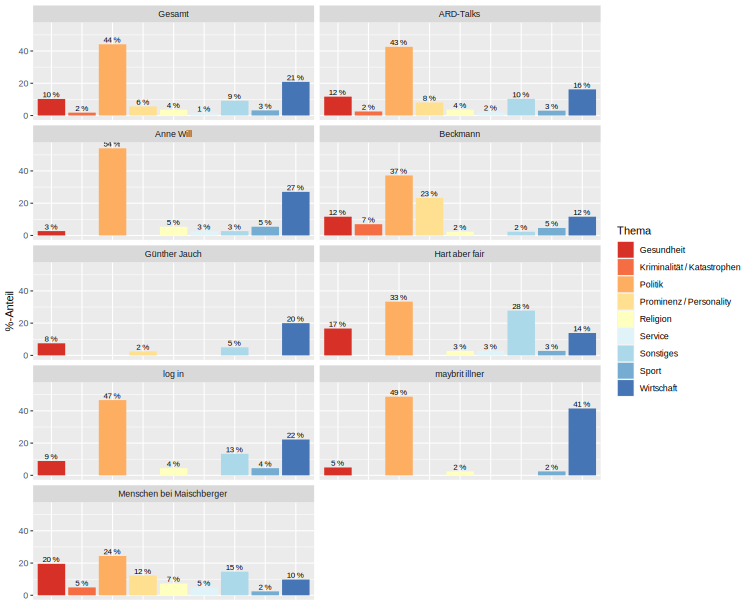
\includegraphics[width=1\textwidth]{daten/grafiken/plot_themenverteilung.png}
	%Captions and Labels can be used since this is a figure environment
	\caption{Themenverteilung innerhalb der Sendungen}
	\subcaption*{vgl. auch ausführliche Tabelle \vref{tab:anhang_themenbereiche_sendungen} im Anhang}
	\label{plot:themenverteilung}
\end{figure}

Wie Abbildung \vref{plot:themenverteilung} zeigt, gibt es dahingegen bei \textit{Beckmann} und \textit{Menschen bei Maischberger} mit ihren relativ geringen Anteilen an politischen und wirtschaftlichen Themen den breitesten Themenmix. Dies zeigt die Nähe der beiden Sendungen zum Personality-Talk und betont zugleich, dass sie thematisch nicht eindeutig dem Polittalk zugeschlagen werden können. Insbesondere \textit{Menschen bei Maischberger} kommt bloß auf einen Politikanteil von 24,4 \%.

Hinsichtlich \textit{hart aber fair} ist der geringe Politik- (33,3 \%) und Wirtschaftsanteil (13,9 \%) und der gleichzeitig relativ breite Themenmix hingegen überraschend, beschreibt sich die Sendung selbst doch als harter Politiktalk. Tatsächlich setzte \textit{hart aber fair} im Untersuchungszeitraum jedoch relativ stark auf Gesundheitsthemen sowie auf Themen, die sich nicht eindeutig einer Kategorie zuordnen ließen. Schaut man sich diese Folgen genauer an, so stellt man fest, dass es sich vor allem um ethische und moralische Fragen handelt. Aber auch exotische Themen werden behandelt, so trug die \textit{hart aber fair} Folge vom 23. April 2012 beispielsweise den Titel „Wissen wo der Hammer hängt – was treibt die Deutschen in den Baumarkt?“.

\textit{log in} unterscheidet sich bei der Themenwahl auf dieser Ebene nicht stark von den anderen Talks. Dies war aber auch nicht unbedingt zu erwarten, schließlich hat die Sendung ebenfalls den Anspruch ein Polittalk zu sein.

Die sieben Sendungen lassen sich anhand der behandelten Themenbereiche in zwei Gruppen einteilen, die sich untereinander nur wenig unterscheiden. In der einen Gruppe finden sich die Sendungen mit relativ hohem Politik- und Wirtschaftsanteil – \textit{Anne Will}, \textit{Günther Jauch} sowie \textit{log in} und maybrit illner. Die zweite Gruppe besteht hingegen aus den Sendungen die einen breiteren Themenmix anbieten – \textit{Beckmann}, \textit{hart aber fair} und \textit{Menschen bei Maischberger}. Wirklich klare Themenprofile, die einer Sendung ein absolutes Alleinstellungsmerkmal geben würden, lassen sich auf dieser Untersuchungsebene nicht feststellen.

\subsubsection{Politikbereiche}

Hinsichtlich der thematisierten Politikbereiche lässt sich festhalten, dass innenpolitische Themen in allen Sendungen klar dominieren (vgl. Abbildung \vref{plot:politikbereiche}), am stärksten bei \textit{Beckmann}, wo fast keine anderen Politikbereiche behandelt werden. \textit{Günther Jauch}, \textit{log in} und \textit{maybrit illner} folgen mit jeweils circa 60 \% Innenpolitikanteil. Einzig \textit{Menschen bei Maischberger} hat genauso oft sozialpolitische wie innenpolitische Themen im Programm. Allerdings ist hier, wie bereits erwähnt, der Anteil politischer Sendungen bereits von vornherein sehr gering. Ähnlich stellt sich die Situation bei hart aber fair dar, hier liegt das Verhältnis von innen- zu sozialpolitischen Themen bei 42 \% zu 33 \%. Einen relativ hohen Anteil an Themen aus dem Bereich der Sozialpolitik hat ebenfalls noch Anne Will (35 \%), allerdings nicht zu Lasten der Innenpolitik, sondern aller anderen Politikbereiche.

Während sich sozialpolitische Thematiken zumindest in allen untersuchten Sendungen fanden, kamen Themen aus dem Bereich der Bildungspolitik gerade einmal in einer Talkshow vor, nämlich in der \textit{Günther Jauch} Folge vom 27. November 2011 mit dem Titel „Generation doof – warum gibt es so viele Bildungsverlierer?“. \textit{Günther Jauch} ist zudem die einzige Sendung, die alle der sechs erfassten Politikbereiche abdeckt. \textit{Beckmann} dagegen behandelt nur innen- und sozialpolitische Themen.

Ebenfalls vernachlässigt werden die Themenbereiche Außen- und Umwelt- bzw. Energiepolitik. \textit{maybrit illner} und \textit{Günther Jauch} kommen immerhin auf zwei Folgen zu außenpolitischen Themen innerhalb eines Jahres und haben damit absolut gesehen den Spitzenplatz inne. Dies ist erstaunlich, hätte es doch innerhalb des Untersuchungszeitraums mehr als genug relevante Anlässe für eine Talkrunde gegeben – man denke nur an die Ereignisse in Ägypten, Tunesien und Libyen im Zuge des sogenannten Arabischen Frühlings.

\begin{figure}[ht]
	%Do not try to scale figure in .tex or you loose font size consistency
	\centering
	%The code to input the plot is extremely simple	
	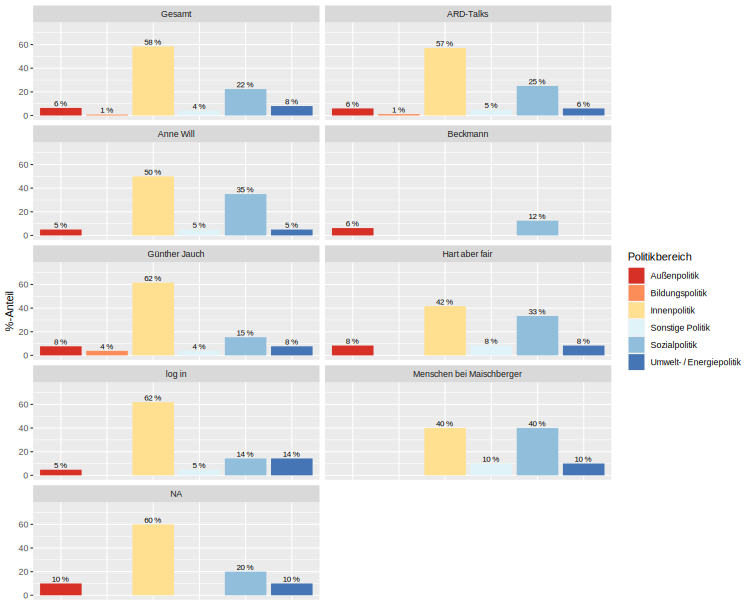
\includegraphics[width=1\textwidth]{daten/grafiken/plot_politikbereiche.png}
	%Captions and Labels can be used since this is a figure environment
	\caption{Politikbereiche nach Sendungen}
	\label{plot:politikbereiche}
	\subcaption*{vgl. auch ausführliche Tabelle \vref{tab:anhang_politikbereiche_sendungen} im Anhang}
\end{figure}

Gleiches gilt für die Umwelt- und Energiepolitik, einzig log in kümmerte sich intensiver um dieses Thema und widmete ihm immerhin drei seiner 21 Talks zu politischen Themen. Damit kann sich die Sendung ein wenig von den anderen untersuchten Talks abheben.

Ergebnisse früherer Untersuchungen werden somit bestätigen \parencite[8f.]{muellerSchaubuehneFuerEinflussreichen2006}: Die Innenpolitik ist sehr dominant, daneben finden eigentlich nur noch sozialpolitischen Themen größere Beachtung in den Sendungen. Alle anderen hier erfassten Politikbereiche – Außen-, Umwelt- bzw. Energiepolitik sowie Bildungspolitik – finden sich hingegen nur selten in den Polittalks. Aus Perspektive der zuvor erläuterten Qualitätskriterien ist dies natürlich problematisch, werden doch hier durchaus wichtige Politikbereiche – etwa die Außenpolitik – stiefmütterlich behandelt und sich fast ausschließlich auf innenpolitische Themen konzentriert. Diese Einseitigkeit setzt sich bei der Themenwahl fort, wie der folgende Abschnitt darlegt.

\subsection{Themencluster}\label{chap:themencluster}

Während die Einteilung in Themenbereiche ein grobes Raster ist, das zwar größere Tendenzen aufzeigen kann – etwa das Vernachlässigen außenpolitischer Fragen – zeigt doch erst eine Einteilung in Themencluster, inwiefern sich Themen tatsächlich wiederholen.

Die häufigsten Themen sind die Eurokrise, mit großem Abstand gefolgt von der sogenannten Wulff-Affäre und dem recht umfassenden Thema Ernährung sowie der Wahl des neuen Bundespräsidenten Joachim Gauck und den beiden sozialpolitischen Themen Renten und soziale Gerechtigkeit – und zwar sowohl im gesamten Sample als auch bei der ARD-Talkschiene alleine (vgl. Tabelle \vref{tab:themencluster}).

\begin{table}[ht]
	\centering
	\caption{Häufige Themencluster}
	\resizebox{\textwidth}{!}{%
		\begin{tabular}{@{}lcccc@{}}
			\toprule
			\multicolumn{1}{c}{\textbf{Themencluster}} & \textbf{Alle Sendungen} & \textbf{Anteil (n=283)} & \textbf{ARD-Talks} & \textbf{Anteil (n=197)} \\ \midrule
			Eurokrise & 47 & 16,6\% & 24 & 12,2\% \\
			Wulff-Affäre & 23 & 8,1\% & 17 & 8,6\% \\
			Ernährung & 11 & 3,9\% & 9 & 4,6\% \\
			Bundespräsident Gauck & 9 & 3,2\% & 7 & 3,6\% \\
			Renten & 8 & 2,8\% & 5 & 2,5\% \\
			Soziale Gerechtigkeit & 8 & 2,8\% & 7 & 3,6\% \\ \bottomrule
		\end{tabular}
	}
	\label{tab:themencluster}
\end{table}

Der Dauerbrenner ist sowohl bei den beiden ZDF-Talks als auch in der ARD-Talkschiene die Eurokrise. In 53 Kalenderwochen des Untersuchungszeitraums wurde mindestens eine der untersuchten Polittalks gesendet. Angesichts von 47 Talkfolgen zur Eurokrise muss man also festhalten, dass dieses Thema theoretisch fast jede Woche Gegenstand der Sendungen war. Nun mag die Eurokrise zwar ein hochdynamisches, komplexes Thema sein, bei dem ein hoher Diskussionsbedarf auch in der Bevölkerung besteht – eine derart häufige Behandlung scheint aber doch übertrieben, dürften hier doch zahlreiche Wiederholungen unvermeidlich sein.

Um herauszufinden, ob es zudem zeitlich begrenzte Themenballungen gab, wurden die Häufigkeit der Themen nach Monaten aufgeschlüsselt. Bei den meisten Themen findet sich eine relativ ausgewogene Verteilung, bei bestimmten spektakulären und kontroversen Themen fanden sich hingegen auffällige Häufungen.

\subsubsection{Die Wulff-Affäre}

Ein solches ist die sogenannte Wulff-Affäre, die sich ab Anfang Dezember 2011 entfaltete und im Rücktritt des damaligen Bundespräsidenten Christian Wulff am 17. Februar 2012 gipfelte. Im Zeitraum vom 14. Dezember 2011 bis zum 11. März 2012 widmen die untersuchten Polittalks diesem Thema allein 23 ihrer Folgen und damit gut 34 \% der in diesem Zeitraum ausgestrahlten Folgen.
Zeitweise fand in den Talks kaum ein anderes Thema statt. In der Woche vom 8. bis zum 12. Januar 2012 hatten beispielsweise fünf der sieben untersuchten Sendungen Wulff zum Thema (vgl. Tabelle \vref{tab:wulff-talks1}).

\begin{table}[ht]
	\centering
	\caption{Talks zur Wulff-Affäre zwischen dem 8. und 12. Januar 2012}
	\resizebox{\textwidth}{!}{%
		\begin{tabular}{@{}lll@{}}
			\toprule
			\multicolumn{1}{c}{\textbf{Datum}} & \multicolumn{1}{c}{\textbf{Sendung}} & \multicolumn{1}{c}{\textbf{Titel}}                                                  \\ \midrule
			8. Januar 2012                     & Günther Jauch                        & Der Problem-Präsident – wie glaubwürdig ist Christian Wulff                         \\
			9. Januar 2012                     & hart aber fair                       & Der Pattex-Präsident – was lehrt der Fall Wulff?                                    \\
			11. Januar 2012                    & log in                               & Liebling, ich habe das Amt geschrumpft - Brauchen wir noch einen Bundespräsidenten? \\
			12. Januar 2012                    & Beckmann                             & Macht, Medien, Moral – wo sind Deutschlands Vorbilder?                              \\
			12. Januar 2012                    & maybrit illner                       & Affäre Wulff: Vorhang zu und viele Fragen offen?                                    \\ \bottomrule
		\end{tabular}
	}
	\label{tab:wulff-talks1}
\end{table}

Als Anfang März die Diskussion über Wulffs Ehrensold aufkam, nahmen das nochmals vier Sendungen zum Anlass innerhalb weniger Tage diesem Thema eine Diskussion zu widmen (vgl. Tabelle \vref{tab:wulff-talks2}).

\begin{table}[ht]
	\centering
	\caption{Talks zur Wulff-Affäre zwischen dem 6. und 11. März 2012}
	\resizebox{\textwidth}{!}{%
		\begin{tabular}{@{}lll@{}}
			\toprule
			\multicolumn{1}{c}{\textbf{Datum}} & \multicolumn{1}{c}{\textbf{Sendung}} & \multicolumn{1}{c}{\textbf{Titel}}                                     \\ \midrule
			6. März 2012                       & Maischberger                         & Ehrensold für Wulff, Millionen für Chefs – und was kriegt der Rest?    \\
			7. März 2012                       & Anne Will                            & Mein Auto, mein Büro, mein Zapfenstreich – Was hat Wulff verdient?     \\
			8. März 2012                       & Beckmann                             & Nach dem Zapfenstreich für Wulff                                       \\
			8. März 2012                       & maybrit illner                       & Versagt, doch gut versorgt? - Wulffs Abschied mit Pauken und Moneten   \\
			11. März 2012                      & Günther Jauch                        & Der tiefe Fall des Christian Wulff – wie gelingt ein Abschied in Würde \\ \bottomrule
		\end{tabular}
	}
	\label{tab:wulff-talks2}
\end{table}

\subsubsection{Bundespräsident Gauck}

Im März 2012 ließ ich eine weitere Themenhäufung feststellen. Innerhalb von  sechs Tagen befassten sich alleine fünf Sendungen mit der (bevorstehenden) Wahl des neuen Bundespräsidenten Joachim Gauck und kaprizierten sich dabei fast ausschließlich auf eine Charakterisierung Gaucks (vgl. Tabelle \vref{tab:gauck-talks}). Eine Häufung die auch dem ARD-Programmbeirat negativ auffiel \parencite[2]{ard-programmbeiratTalkformateImErsten2012}.

\begin{table}[ht]
	\centering
	\caption{Talks zur Bundespräsidentenwahl zwischen 14. und 19. März 2012}
	\resizebox{\textwidth}{!}{%
		\begin{tabular}{@{}lll@{}}
			\toprule
			\multicolumn{1}{c}{\textbf{Datum}} & \multicolumn{1}{c}{\textbf{Sendung}} & \multicolumn{1}{c}{\textbf{Titel}}                                        \\
			\midrule
			14. März 2012                      & Anne Will                            & Bundespräsident Gauck – bekommen wir endlich den Richtigen?               \\
			15. März 2012                      & Beckmann                             & Die Präsidentenmacher – Drei Tage vor der Wahl des neuen Staatsoberhaupts \\
			15. März 2012                      & maybrit illner                       & Gauck for President - fast alle für einen, einer für alle?                \\
			18. März 2012                      & Günther Jauch                        & Joachim Gauck – der Volks-Präsident                                       \\
			19. März 2012                      & hart aber fair                       & Der Bewährungshelfer – kann Gauck das Ansehen der Politiker heilen?       \\
			\bottomrule
		\end{tabular}
	}
	\label{tab:gauck-talks}
\end{table}

Derartige Themenballungen lassen sich immer wieder – wenn auch meist in kleinerem Umfang – im Beobachtungszeitraum finden. Zum Beispiel beschäftigten sich innerhalb von fünf Wochen zwei Talks mit dem Thema Burnout – wobei in diesem Fall nicht zu erwarten ist, dass sich innerhalb dieser Zeit neue Erkenntnis ergeben haben.

Bei einigen Themen wird man dies zwar dadurch rechtfertigen können, dass das Thema aus einem anderen Blickwinkel beleuchtet wird, die Sendungen stark unterschiedliche Zielgruppen ansprechen oder das Thema eine solche Relevanz besitzt, dass eine mehrmalige Thematisierung lohnt. Häufungen wie zuvor exemplarisch dargestellt, wenn sich also innerhalb eines kurzen Zeitraums fast alle Sendungen dem gleichen Thema widmen, lassen sich so allerdings nicht rechtfertigen. Hier ist schlicht und ergreifend ermüdende Wiederholung des immer gleichen an der Tagesordnung, während andere – eventuell genauso relevante Themen – nicht behandelt werden und damit auch von einer pluralen Themensetzung keine Rede mehr sein kann.

\subsection{Titelgebung}\label{chap:titelgebung}

Nicht systematisch untersucht wurde die Titelgebung der einzelnen Talkshowfolgen. Ein Blick auf den Korpus macht dennoch deutlich, dass viele Titel Formulierungen benutzen, die einen Skandal oder eine drohende Katastrophe suggerieren und damit Angst wecken bzw. zumindest provokativ wirken.

Meist wird dem Titel ein Fragezeichen nachgestellt, um so den Eindruck einer ergebnisoffenen Diskussion zu erwecken was allerdings meist schon durch den Rest des Titels konterkariert wird. Besonders deutlich wird dies, wenn man die Titel mit denen älterer Sendungen vergleicht. \textcite[195f.]{kellerGeschichteTalkshowDeutschland2009} gibt einige Titel aus den 1960er Jahren wieder, diese zeichnen sich meist durch neutrale und einfache Frageformulierungen aus – etwa: „Lässt sich Bildung planen?“\footnote{Zugegebenermaßen finden sich solche Titel bereits in der großen politischen Talkshow der 90er Jahre, Talk im Turm, seltener \parencite[301f.]{kellerGeschichteTalkshowDeutschland2009}.}. Heutige Titel versuchen dagegen durch Emotionalisierung die Zuschauer anzusprechen, dramatisieren damit aber von vornherein die Themen und schränken die Diskussion zudem durch Vorfestlegungen bereits im Vorhinein ein.

Tabelle \vref{tab:talktitel} dokumentiert eine kleine Auswahl an exemplarischen Titeln, die obigen Befund veranschaulichen:

\begin{table}[ht]
	\centering
	\caption{Ausgewählte Titelbeispiele}
	\resizebox{\textwidth}{!}{%
		\begin{tabular}{@{}lll@{}}
			\toprule
			\multicolumn{1}{c}{\textbf{Datum}} & \multicolumn{1}{c}{\textbf{Sendung}} & \multicolumn{1}{c}{\textbf{Titel}}                                                \\ \midrule
			  25. April 2012 & Anne Will & Preis-Wahnsinn an der Zapfsäule – Autofahren bald unbezahlbar? \\
			  24. November 2011& Beckmann & Krankenhaus-Keime – Die unsichtbare Gefahr \\
			  9. Oktober 2011& Günther Jauch & Essen für die Tonne – wie stoppen wir den Wegwerf-Wahnsinn? \\
			  16. Juli 2012& hart aber fair& Umsorgt vom Kreißsaal bis zum Hörsaal – kommt jetzt die Generation Weichei? \\
			  29. Februar 2012 & log in& Teuro-Sprit und Turbo-Protzer – Sind Autos von gestern? \\
			  6. Oktober 2012& maybrit illner& Burnout – muss bald ganz Deutschland auf die Couch?\\
			  27. September 2011 & Maischberger & Machofrauen – Müde Männer: Letzte Runde im Geschlechterkampf? \\ \bottomrule
		\end{tabular}
	}
\label{tab:talktitel}
\end{table}

\section{Gästestruktur}

Nachdem die Themenstruktur bereits gewisse Einseitigkeiten und Unzulänglichkeiten offenbart hat, wird im Weiteren die Gästestruktur der gleichen Analyse unterzogen.

\subsection{Personenspektrum}\label{chap:personenspektrum}

Bei der Untersuchung der Gästestruktur ist zuvorderst die Frage interessant, ob die  Talkshows – wie ihnen regelmäßig vorgeworfen wird – immer wieder die gleichen Personen einladen. Ob also eine Art „Talkelite“ besteht und diese somit bevorzugt ihre Interessen und Meinungen den Zuschauern präsentieren können\footnote{Natürlich lassen sich aufgrund der Ergebnisse nur bedingt Aussagen zum Prozess der Gästeauswahl treffen. So ist es prinzipiell möglich, dass die verschiedenen Redaktionen sich durchaus bemühen ein plurales Gästespektrum sicher zu stellen, ihre Bemühungen aber aufgrund von Absagen und ähnlichem scheitern.}.

\subsubsection{Alle Sendungen}

Insgesamt waren in allen erfassten Sendungen 1441 Gäste eingeladen. Etwas mehr als die Hälfte davon nur einmal (753), zweimal waren 120 Personen eingeladen, dreimal  44 und viermal 23. Fünf- bzw. sechsmal waren noch 15 bzw. 10 Personen eingeladen.

Die Gästeliste wird angeführt von elf Personen, die zwischen sieben und elfmal an einer politischen Talkshow teilnahmen. Zusammen bestreiten diese Personen etwa zehn Prozent der Auftritte. Die Spitzenposition hat dabei CDU-Arbeits- und Sozialministerin Ursula von der Leyen inne. Von den elf Personen sind wiederum acht Politiker (vgl. Tabelle \vref{tab:gaesterangliste}). Wir werden später noch sehen, dass oftmals die gleichen Politiker eingeladen werden. Die Bedeutung der Werte wird klar, wenn man sich vor Augen führt, dass innerhalb des Untersuchungszeitraums in 53 Wochen Polittalks ausgestrahlt wurden, das heißt, dass beispielsweise Ursula von der Leyen rein statistisch in elf dieser 53 Wochen als Gast in einer der sieben Talkshows zugegen war. Dies wären immerhin etwa 30 \% des Untersuchungszeitraums.

\begin{table}[ht]
	\centering
	\caption{Gästerangliste}
%	\resizebox{\textwidth}{!}{%
		\begin{tabular}{@{}llll@{}}
			\toprule
			\multicolumn{1}{c}{\textbf{Gast}} & \multicolumn{1}{c}{\textbf{Rolle}} & \multicolumn{1}{c}{\textbf{Auftritte}} & \multicolumn{1}{c}{\textbf{Anteil}} \\ \midrule
			Ursula von der Leyen              & Politiker                          & 11                                     & 0,76\%                              \\
			Wolfgang Bosbach                  & Politiker                          & 10                                     & 0,69\%                              \\
			Dirk Müller                       & Finanzexperte                      & 9                                      & 0,62\%                              \\ 
			Peter Altmaier                    & Politiker                          & 9                                      & 0,62\%                              \\
			Sahra Wagenknecht                 & Politikerin                        & 9                                      & 0,62\%                              \\
			Hans-Ulrich Jörges                & Journalist                         & 8                                      & 0,56\%                              \\
			Christian Lindner                 & Politiker                          & 7                                      & 0,49\%                              \\
			Gertrud Höhler                    & Publizistin                        & 7                                      & 0,49\%                              \\
			Gregor Gysi                       & Politiker                          & 7                                      & 0,49\%                              \\
			Jürgen Trittin                    & Politiker                          & 7                                      & 0,49\%                              \\
			Wolfgang Kubicki                  & Politiker                          & 7                                      & 0,49\%                              \\
			10 Gäste                          &                                    & 6                                      & 4,16\%                              \\
			15 Gäste                          &                                    & 5                                      & 5,20\%                              \\
			23 Gäste                          &                                    & 4                                      & 6,38\%                              \\
			44 Gäste                          &                                    & 3                                      & 9,16\%                              \\
			120 Gäste                         &                                    & 2                                      & 16,52\%                             \\
			751 Gäste                         &                                    & 1                                      & 52,26\%                             \\
			\midrule
			&                                    &                                        & 100,00\% \\
			\bottomrule                           
		\end{tabular}
%	}
	\subcaption*{alle Sendungen; n=1441}
	\label{tab:gaesterangliste}
\end{table}

\subsubsection{Die Sendungen im Vergleich}

Betrachtet man die Sendungen getrennt voneinander, so ergibt sich ein differenzierteres Bild. Um aussagekräftigere und leichter vergleichbare Ergebnisse zu erzielen, wurde ein Wiederholungsquotient errechnet. Hierzu wurde die Anzahl an Gästen durch die Anzahl an individuellen Personen dividiert. Hierdurch erhält man eine Zahl zwischen 1 und x. Wenn der Quotient 1 ist heißt das, dass die Zahl der Auftritte mit der Zahl individueller Personen identisch ist, mithin jeder Talkgast bloß einmal eingeladen war. Ist das Ergebnis hingegen zwei, so bedeutet dies, dass im Durchschnitt jede Person zweimal zu Gast war.
 
\begin{figure}[ht]
	%Do not try to scale figure in .tex or you loose font size consistency
	\centering
	%The code to input the plot is extremely simple
	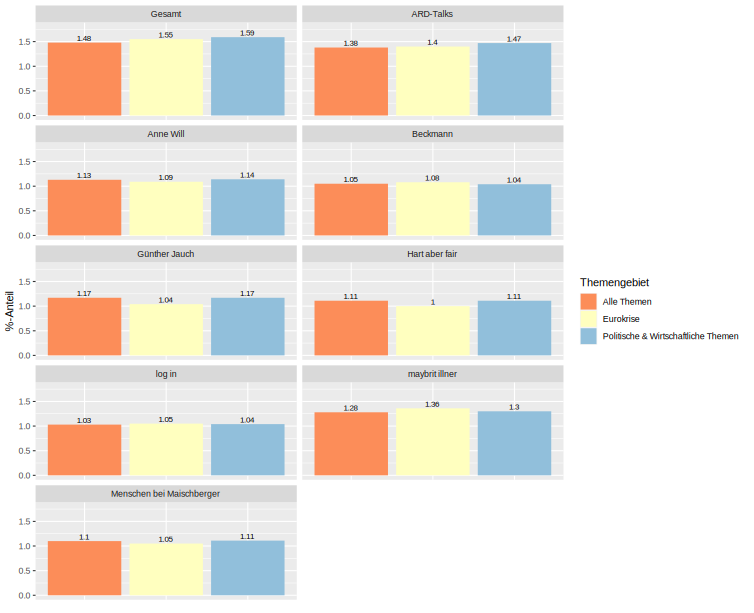
\includegraphics[width=1\textwidth]{daten/grafiken/plot_wdhquote_gaeste.png}
	%Captions and Labels can be used since this is a figure environment
	\caption{Wiederholungsquotient (alle Gäste)}
	\label{plot:whdquote_gaeste}
\end{figure}

Wie bei Betrachtung von Abbildung \vref{plot:whdquote_gaeste} deutlich wird, gibt es zwischen den einzelnen Sendungen teils deutliche Unterschiede. Während bei \textit{log in} und \textit{Beckmann} nur äußerst selten Gäste mehrfach auftauchen, findet sich bei \textit{maybrit illner} ein relativ hoher Quotient von 1,28 – sprich es traten innerhalb der Sendung häufiger Personen mehrfach auf als in den anderen Polittalks.

Dennoch sind die Quotienten innerhalb der Sendungen gering im Vergleich zu denen zwischen den Sendungen. Sowohl innerhalb der ARD-Talkschiene als auch zwischen allen untersuchten Polittalks kommt es zu häufigeren Gästewiederholungen. Dies spricht dafür, dass die einzelnen Redaktionen zwar darauf achten, dass innerhalb ihrer Sendung nicht allzu oft die gleichen Personen auftreten, dies aber zwischen den Sendungen nicht gelingt.

Besonders auffällig ist, dass der Wiederholungsquotient bei politischen und wirtschaftlichen Themen bei fast allen Sendungen höher ist als im Gesamtschnitt. Über alle Sendungen hinweg beträgt der Quotient hier fast 1,6, was darauf hindeutet, dass es bei politischen und wirtschaftlichen Themen tatsächlich eine Art Talkelite gibt, die zwar nicht unbedingt immer wieder in der gleichen Sendung zu Gast ist, dafür stattdessen durch alle Sendungen tingelt.

Ähnliches gilt hinsichtlich der Wiederholungsquote bei Talks zur Eurokrise. Auch dort liegt der Quotient bei den einzelnen Sendungen meist relativ niedrig, oftmals sogar niedriger als im Gesamtschnitt. Über alle Sendungen hinweg hingegen ist die Wiederholungsquote mit 1,55 dagegen fast genauso hoch wie bei den politischen und wirtschaftlichen Themen.

\subsubsection{Politische Talkelite – Talkende Politikerelite}

Das obige Ergebnis wird noch verstärkt, wenn die Gäste nach ihren Funktionen getrennt betrachtet werden. Hier wird erneut bestätigt, dass es eine Art Politikelite gibt, die immer wieder eingeladen wird. So treten zwar in den untersuchten Sendungen 424-mal Politiker auf, diese Auftritte werden aber nur von 196 unterschiedlichen Personen bestritten (vgl. Tabelle \vref{tab:poltikerauftritte}).

\begin{table}[ht]
	\centering
	\caption{Auftritte von Politikern}
	\resizebox{\textwidth}{!}{%
		\begin{tabular}{@{}lll@{}}
			\toprule
			\multicolumn{1}{c}{\textbf{Gäste}} & \multicolumn{1}{c}{\textbf{Anzahl an Auftritte}} & \multicolumn{1}{c}{\textbf{\%-Anteil an den Auftritten}} \\ \midrule
			Ursula von der Leyen & 11 & 2,6\%   \\
			Wolfgang Bosbach & 10  & 2,4\%   \\
			2 Politiker & Je 9 & 4,3\%   \\
			4 Politiker & Je 7 & 6,6\%   \\
			6 Politiker & Je 6 & 8,5\%   \\
			8 Politiker & Je 5 & 9,4\%   \\
			13 Politiker & Je 4 & 12,3\%  \\
			15 Politiker & Je 3 & 10,6\%  \\
			38 Politiker & Je 2 & 17,9\%  \\
			108 Politiker & Je 1 & 25,5\%  \\ \midrule
			Insgesamt 196 & Insgesamt 424 & 100,0\% \\ \bottomrule
		\end{tabular}
	}
	\label{tab:poltikerauftritte}
\end{table}

Dies ergibt einen Wiederholungsquotienten von 2,16 und bedeutet das im Durchschnitt jeder Politiker mehr als zweimal in den Polittalks auftrat. Bei Journalisten beträgt der Wert nur noch 1,56, bei Experten und Wirtschaftsvertretern noch 1,35 bzw. 1,34. Vertreter von Religionsgemeinschaften und Normalbürger sind fast ausschließlich nur einmal Gast in den untersuchten Sendungen (vgl. Abbildung \vref{plot:whdquote_gaeste_allg}). Die Beschränkung auf wenige Personen mit häufigem Erscheinen ist also nicht bei allen Gästegruppen gleich stark ausgeprägt.

\begin{figure}[ht]
	%Do not try to scale figure in .tex or you loose font size consistency
	\centering
	%The code to input the plot is extremely simple
	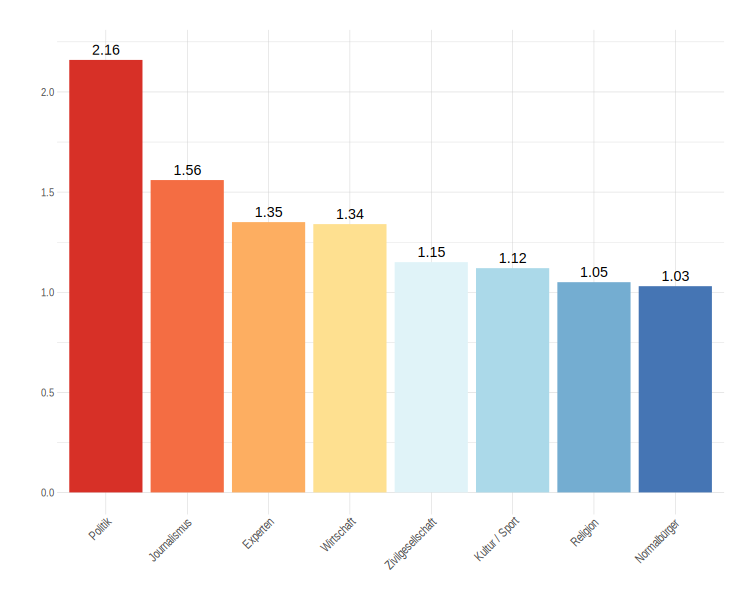
\includegraphics[width=1\textwidth]{daten/grafiken/plot_wdhquote_gaeste_allg.png}
	%Captions and Labels can be used since this is a figure environment
	\caption{Wiederholungsquotient (Auftritte / Personen) nach Rollen}
	\label{plot:whdquote_gaeste_allg}
\end{figure}

\subsubsection{Talkelite in der Eurokrise}

Doch findet sich dieses Bild bei allen Themen? Ein Blick auf die Situation beim Thema Eurokrise bestätigt dies nicht. Zwar liegt auch hier der Wiederholungsquotient bei Politikern am höchsten, gleichzeitig ist er aber zum einen um 0,46 Punkte niedriger und zum anderen liegt er insbesondere bei Experten und Vertretern aus dem Bereich Wirtschaft nun deutlich höher (vgl. Abbildung \vref{plot:whdquote_gaeste_euro}).

Die Vermutung liegt nahe, dass es also je nach Thema unterschiedliche Talkeliten gibt. Eine entsprechende Analyse kann an dieser Stelle leider nicht für jedes Thema erfolgen, da dies den Rahmen sprengen würde. Bei Talks zur Eurokrise jedenfalls findet sich statt einer reinen Politikerelite, vielmehr eine Gästeelite aus Experten und Personen aus den Bereichen Politik und Wirtschaft.

\begin{figure}[ht]
	%Do not try to scale figure in .tex or you loose font size consistency
	\centering
	%The code to input the plot is extremely simple
	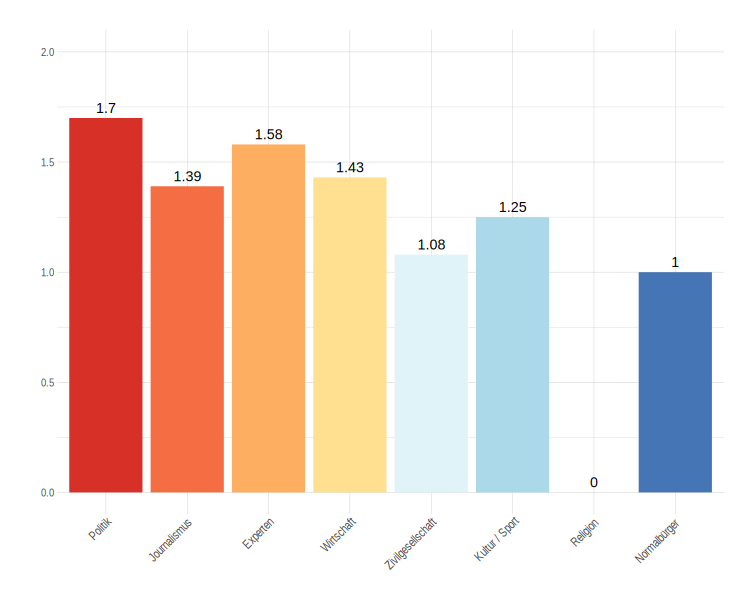
\includegraphics[width=1\textwidth]{daten/grafiken/plot_wdhquote_gaeste_euro.png}
	%Captions and Labels can be used since this is a figure environment
	\caption{Wiederholungsquotient (Auftritte / Personen) nach Rollen (Eurokrise)}
	\label{plot:whdquote_gaeste_euro}
\end{figure}

\subsection{Gesellschaftliche Rollen}\label{chap:gesellschaftlicherollen}

Bei der Analyse politischer Talkshows sind nicht nur einzelne Personen und die Häufigkeit ihres Auftretens interessant, sondern auch welche gesellschaftlichen Rollen diese Personen vertreten und ob sich hier eventuell ebenfalls Einseitigkeiten feststellen lassen\footnote{Da Personen durchaus mehrere gesellschaftliche Rollen inne haben können, erfolgte die Zuordnung zu den Kategorien jeweils auf Basis der Vorstellung der jeweiligen Gäste in den Sendungen bzw. auf der zugehörigen Internetseite. Dies ist insofern sinnvoll, als man davon ausgehen kann, dass die jeweiligen Personen aufgrund dieser gesellschaftlichen Rolle in die Sendung eingeladen wurden.}.

\subsubsection{Gesamtbild}

Die in Tabelle \vref{tab:prozent-rollen} aufgeführte prozentuale Rollenverteilung zeigt, dass insgesamt Politiker am häufigsten eingeladen waren, also genau die Gruppe deren individuelle Vertreter oft mehrmals eingeladen wurden (vgl. Kapitel \vref{chap:personenspektrum}). Mit über zehn Prozentpunkten Abstand folgen dicht beieinander Personen aus dem kulturellen und sportlichen Bereich, Experten und Journalisten. Knapp dahinter liegen Wirtschaftsvertreter mit circa zehn Prozent. Weit seltener zu Gast waren wiederum „Normalbürger“, Vertreter der Zivilgesellschaft – also von Vereinen, Verbänden oder Non Governmental Organisations (NGOs) – und von Religionsgemeinschaften.

Ähnlich stellt sich die Verteilung dar, wenn nur die Sendungen der ARD-Talkschiene betrachtet werden. Zwar werden etwas häufiger Personen aus dem Bereich Journalismus, Kultur / Sport, sowie Experten und „Normalbürger“ eingeladen und etwas seltener aus  Wirtschaft, Zivilgesellschaft und Politik. Die Unterschiede bewegen sich aber im ein bis zweistelligen Prozentbereich und sind damit marginal. Dennoch kann insgesamt nicht von einer Dominanz aller Sendungen durch Politiker die Rede sein, machen sie doch insgesamt weniger als ein Drittel der Gäste aus.

\begin{table}[ht]
	\centering
	\caption{Prozentuale Rollenverteilung}
	\resizebox{\textwidth}{!}{%
		\begin{tabular}{@{}lllll@{}}
			\toprule
			&
			\multicolumn{1}{c}{\textbf{\begin{tabular}[c]{@{}c@{}}Alle Folgen\\ (n=1441)\end{tabular}}} &
			\multicolumn{1}{c}{\textbf{\begin{tabular}[c]{@{}c@{}}ARD-Talkschiene\\ (n=1044)\end{tabular}}} &
			\multicolumn{1}{c}{\textbf{\begin{tabular}[c]{@{}c@{}}Politische Themen\\ (n=640)\end{tabular}}} &
			\multicolumn{1}{c}{\textbf{\begin{tabular}[c]{@{}c@{}}Eurokrise\\ (n=229)\end{tabular}}} \\ \midrule
			\textbf{Politik}           & 29,40\%  & 26,10\%  & 39,70\%  & 44,50\%  \\
			\textbf{Kultur / Sport}    & 16,10\%  & 18,50\%  & 12,00\%  & 2,20\%   \\
			\textbf{Experten}          & 15,60\%  & 16,50\%  & 10,80\%  & 16,60\%  \\
			\textbf{Journalismus}      & 14,70\%  & 16,10\%  & 16,40\%  & 17,00\%  \\
			\textbf{Wirtschaft}        & 9,90\%   & 9,20\%   & 9,40\%   & 13,10\%  \\
			\textbf{„Normalbürger“}    & 7,40\%   & 8,60\%   & 5,30\%   & 0,90\%   \\
			\textbf{Zivilgesellschaft} & 5,30\%   & 3,40\%   & 5,60\%   & 5,70\%   \\
			\textbf{Religion}          & 1,50\%   & 1,50\%   & 0,80\%   & 0,00\%   \\
			\textbf{Sonstige}          & 0,10\%   & 0,10\%   & 0,00\%   & 0,00\%   \\
			\midrule
			\textbf{Alle Sendungen}    & 100,00\% & 100,00\% & 100,00\% & 100,00\% \\ \bottomrule
		\end{tabular}
	}
	\label{tab:prozent-rollen}
\end{table}

Bei den Talks zum Thema Eurokrise bzw. allgemein zu politischen Themen kann hingegen von einer derartigen Dominanz gesprochen werden. Dort kommen 44,5 \% respektive 39,7 \% der Gäste aus dem Politikbetrieb. Ebenfalls stärker als im Gesamtschnitt sind Personen aus der Wirtschaft anwesend. Vertreter von Religionsgemeinschaften, aus dem Bereich des kulturellen und sportlichen Lebens, sowie „Normalbürger“ sind gar nicht oder sehr selten eingeladen. Angesichts des Themas ist dies allerdings nicht verwunderlich.

Bei politischen Themen im Allgemeinen machen „Normalbürger“ hingegen immerhin 5,3 \% der Gäste aus – und damit fast genauso viele wie die Repräsentanten der Zivilgesellschaft. Etwas seltener als im Gesamtschnitt in den Runden zugegen sind Gäste aus Kultur und Sport, sowie überraschenderweise Experten, die bei der Eurokrise noch über dem Durchschnitt aller Folgen lagen.

\subsubsection{Sendungen im Vergleich}

\begin{figure}[ht]
	%Do not try to scale figure in .tex or you loose font size consistency
	\centering
	%The code to input the plot is extremely simple
	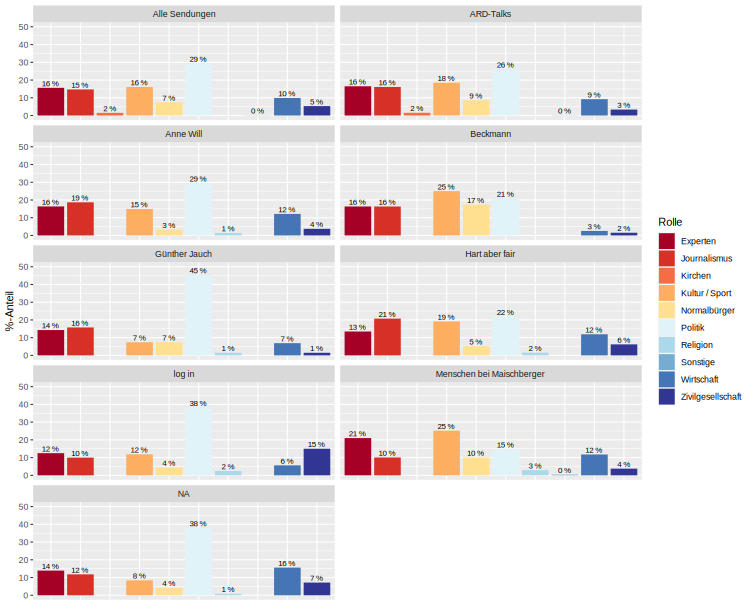
\includegraphics[width=1\textwidth]{daten/grafiken/plot_rollenverteilung.png}
	%Captions and Labels can be used since this is a figure environment
	\caption{Prozentuale Rollenverteilung (nach Sendungen getrennt)}
	\subcaption*{(vgl. auch ausführliche Tabelle \vref{tab:anhang_gaestegruppen_sendungen} im Anhang)}
	\label{plot:rollenverteilung}
\end{figure}

Differenziert man wiederum nach Sendungen so werden einige Unterschiede deutlich, die auf die unterschiedlichen Ausrichtungen der Polittalks hindeuten (vgl. Abbildung \vref{plot:rollenverteilung}). Das Flaggschiff der ARD, \textit{Günther Jauch}, gibt sich erwartungsgemäß ähnlich parteinah wie früher \textit{Sabine Christiansen} \parencite[4f.]{muellerSchaubuehneFuerEinflussreichen2006}, und erreicht einen Anteil von über 45 \% bei den Gästen aus dem politisch-administrativen Bereich. Hier kann entsprechend tatsächlich von einer Politikerdominanz der Gästestruktur gesprochen werden. Ähnlich hohe Werte erreichen noch \textit{maybrit illner} und – überraschenderweise – \textit{log in} mit je circa 38 \%. Somit unterscheidet sich das junge Format gerade nicht durch die gesellschaftlichen Rollen seiner Gäste von den etablierten politischen Talkshows. Allerdings hat die Sendung einen hohen Anteil zivilgesellschaftlicher Akteure unter den Gästen.

Bei den beiden „weicheren“ Formaten \textit{Beckmann} und \textit{Menschen bei Maischberger} sind hingegen nicht Politiker die häufigste Gästegruppe, sondern Personen aus dem kulturellen und sportlichen Leben. Zudem finden überdurchschnittlich oft „Normalbürger“ in den Sendungen Gehör. Hiermit können sich beide von den übrigen fünf Sendungen absetzen und unterstreichen nochmals ihre Nähe zum Personality-Talk.

Ebenfalls auffallend ist die Ähnlichkeit der Gästestrukturen von hart aber fair zu \textit{Maischberger} und \textit{Beckmann}. Obwohl vom Selbstverständnis her viel stärker dem klassischen Polittalk nachempfunden, ist der Anteil politischer Gäste nur unwesentlich größer als bei \textit{Beckmann}. Gäste aus dem Bereich Kultur und Sport sind zudem die dritthäufigste Gästegruppe, wir werden im zweiten Teil der Arbeit noch sehen, dass diese Einladungen nicht immer sinnvoll sind. Es zeigt sich damit bei hart aber fair das gleiche Bild, das sich bereits bei der Themenanalyse abzeichnete.

Im nächsten Schritt werden ausgewählte Gästegruppen nochmals en Detail betrachtet. Vertreter von Religionsgemeinschaften und sonstige Gäste sind kaum unter den Teilnehmern, so dass hier auf eine detaillierte Aufschlüsselung im Folgenden verzichtet wird. Gleiches gilt für „Normalbürger“ und Personen aus dem Bereich Kultur / Sport, deren Detailanalyse für die Beantwortung der behandelten Fragestellungen keinen Gewinn verspricht.

\subsubsection{Politikebenen}

Dass Politiker die größte Gästegruppe ausmachen wurde bereits festgestellt, schaut man sich nun diese Gruppe genauer an, so zeigt sich, dass es sich wiederum hauptsächlich um Personen aus der Bundespolitik handelt (vgl. Abbildung \vref{plot:politikebenen}). Von 424 Politikern sind 289 (68 \%) solche die auf der Bundesebene politische Ämter innehaben bzw. hatten. Nur 96 (23 \%) sind Landespolitiker und nochmals weit weniger sind auf EU- bzw. kommunalpolitischer Ebene aktiv, nämlich 17 (4 \%) bzw. 7 (2 \%). Ausländische Politiker treten nur viermal (1 \%) auf. Die Unterschiede zwischen den einzelnen Sendungen sind marginal, sodass auf eine differenzierte Darstellung verzichtet wird. Ebenfalls kaum in Erscheinung treten Behördenvertreter (2 \%).

\begin{figure}[ht]
	%Do not try to scale figure in .tex or you loose font size consistency
	\centering
	%The code to input the plot is extremely simple
	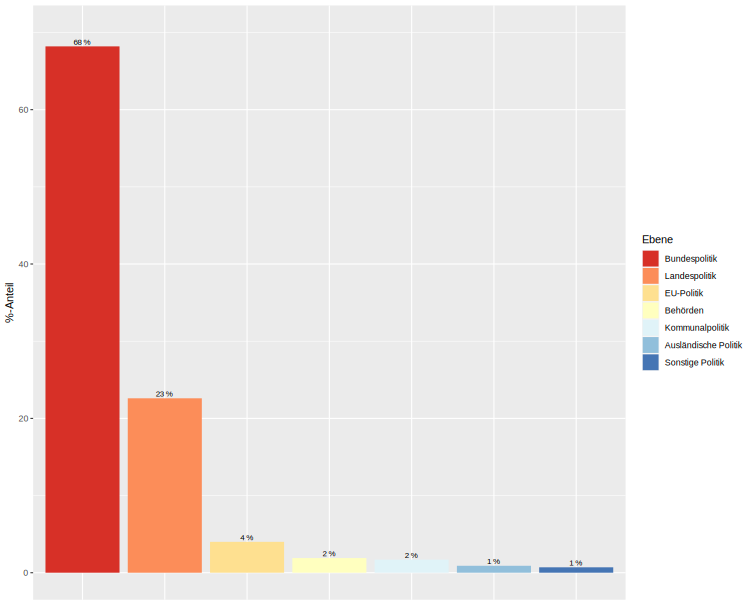
\includegraphics[width=1\textwidth]{daten/grafiken/plot_politikebenen.png}
	%Captions and Labels can be used since this is a figure environment
	\caption{Rollenverteilung innerhalb der Kategorie \textit{Politik} (n=424)}
	\label{plot:politikebenen}
\end{figure}

Dieses Übergewicht der Bundespolitik ist in mehrerlei Hinsicht problematisch. Erstens ist das hiesige politische System stark föderal geprägt, die Länder spielen im politischen Entscheidungssystem eine große Rolle, und zwar auch bei vornehmlich bundespolitischen Themen \parencite[303-331]{rudzioPolitischeSystemBundesrepublik2006}. Der geringe Anteil an Landespolitikern in den untersuchten Talkshows kann also beim Publikum ein falsches Bild über die Rolle bundespolitischer Akteure hervorrufen. Zudem gibt es zwischen den einzelnen Bundesländern Konflikte zum Beispiel über den Länderfinanzausgleich die einer öffentlichen Diskussion durchaus wert sind. Auch kommunalpolitische Themen, wie die Überschuldung der Kommunen, haben nationale Relevanz und würden eine verstärkte Einladung von Politiker aus Kommunal- und Landespolitik rechtfertigen\footnote{Zwar wurde bei der Themenanalyse nicht erfasst auf welche Politikebene sich diese beziehen, allerdings betreffen viele Themen prinzipiell auch die Bundesländer, sodass eine Unterscheidung hier per se sehr schwierig geworden wäre.}.

Zweitens tangieren Entscheidungen in Brüssel Deutschland als EU-Mitgliedsstaat. Teilweise haben dabei Entscheidungen, die von Kommission oder Europäischem Parlament getroffen werden, weitreichende Auswirkungen auf die nationale Ebene \parencite{sturmNeueDeutscheRegierungssystem2005}. Auch hier korrespondiert also nicht die Häufigkeit der Auftritte mit der tatsächlichen Wichtigkeit der Ebene im politischen Prozess. Hinzu kommt, dass der EU weiterhin die Akzeptanz in der Bevölkerung fehlt, so ist beispielsweise die Beteiligung bei den Europawahlen seit 1979 fast durchgängig gesunken \parencite{bundeszentralefuerpolitischebildungEuropawahlWahlbeteiligung197920092009}, und gleichzeitig EU-Vertreter in den Medien unterproportional häufig vorkommen \parencite{roschMedienHabenNachholbedarf2008}. Aufgabe der Polittalks wäre es in diesem Zusammenhang durch die häufigere Einladung von EU-Parlamentariern oder sonstigen Vertretern der EU diesen Effekten entgegen zu wirken, statt sie schlicht zu reproduzieren.

Ähnliches gilt für die Einladung ausländischer Politiker, die das Potenzial hätten, die Diskussion um außerdeutsche Perspektiven zu erweitern, was gerade bei der Eurokrise  sinnvoll erscheint. Doch scheuen die Redaktionen wohl den hiermit verbundenen Aufwand. so dass selbst Politiker aus den direkten Nachbarländern so gut wie nie zu Gast sind\footnote{Die ausländischen Politiker, die in den untersuchten Sendungen zu Gast waren, sind Avi Primor, der ehemalige Botschafter Israels in Deutschland, Richard Sulik, der zum damaligen Zeitpunkt Präsident des slowakischen Parlaments war und Tim Guldimann, der Schweizer Botschafter in Deutschland. Alle drei sprechen fließend deutsch und sind somit unkomplizierte Gäste.}.

Die Dominanz der Bundesebene spricht zudem dafür, dass weiterhin vor allem die politische Elite eingeladen wird \parencite[141]{doernerPolitainmentPolitikMedialen2001}.

\subsubsection{Wirtschaft}

Ebenfalls näher betrachtet werden sollen hier die Gäste aus dem wirtschaftlichen Leben, kann es doch innerhalb dieser Gruppe enorme Interessengegensätze geben. Der wichtigste ist hierbei der zwischen Kapital und Arbeit, sprich zwischen Unternehmensvertreter und Arbeitnehmer respektive ihren jeweiligen Verbänden bzw. Gewerkschaften. Von politischen Talkshows im öffentlich-rechtlichen Fernsehen wäre entsprechend zu erwarten, dass sie zumindest für ein ausgeglichenes Verhältnis zwischen beiden Seiten sorgen.

Allerdings zeigt sich ein klares Übergewicht der Arbeitgeberseite (vgl. Tabelle \vref{tab:gaeste_wirtschaft}). In sechs der sieben Sendungen waren mehr Vertreter von Unternehmen bzw. Wirtschaftsverbänden zu Gast als Gewerkschafter und Arbeitnehmer. Teilweise beträgt der Unterschied weit über 50 \%. So kommen beispielsweise in der Sendung mit dem höchsten Anteil von Gästen aus dem Bereich Wirtschaft, \textit{maybrit illner}, 62 \% mehr wirtschaftsnahe Personen zu Wort als Arbeitnehmer (-vertreter). \textit{log in} ist die einzige positive Ausnahme, der Unterschied beträgt hier nur 11,1 \% zu Lasten der arbeitnehmernahen Positionen. Allerdings kommen bei \textit{log in} insgesamt nur neun Gäste aus dem Bereich Wirtschaft vor. Noch weniger wurden nur zu \textit{Beckmann} eingeladen, dort traten fünf Vertreter von Unternehmen, zwei von Wirtschaftsverbänden und niemand von Arbeitnehmerseite auf.

Eine noch krassere Ungleichverteilung gibt es bei den Talks zur Eurokrise. Dort kommen nur bei \textit{maybrit illner} Vertreter von Arbeitnehmerseite vor und auch dann nur zwei Stück, im Gegensatz zu vierzehn von Arbeitgeberseite.

\begin{table}[ht]
	\centering
	\caption{Gäste aus dem Bereich Wirtschaft (alle Sendungen)}
	\resizebox{\textwidth}{!}{%
		\begin{tabular}{@{}ccccc@{}}
			\toprule
			&
			\textbf{Unternehmen} &
			\textbf{Wirtschaftsverband} &
			\textbf{Gewerkschaft} &
			\textbf{Arbeitnehmer} \\ \midrule
			\textbf{\begin{tabular}[c]{@{}c@{}}Anne Will\\ (n=26)\end{tabular}} &
			50,00 \% &
			23,10 \% &
			11,50 \% &
			15,40 \% \\
			\textbf{\begin{tabular}[c]{@{}c@{}}Beckmann\\ (n=5)\end{tabular}} &
			80,00 \% &
			20,00 \% &
			0,00 \% &
			0,00 \% \\
			\textbf{\begin{tabular}[c]{@{}c@{}}Günther Jauch\\ (n=14)\end{tabular}} &
			80,00 \% &
			20,00 \% &
			0,00 \% &
			0,00 \% \\
			\textbf{\begin{tabular}[c]{@{}c@{}}hart aber fair\\ (n=23)\end{tabular}} &
			43,50 \% &
			34,80 \% &
			13,00 \% &
			8,70 \% \\
			\textbf{\begin{tabular}[c]{@{}c@{}}log in\\ (n=9)\end{tabular}} &
			33,30 \% &
			22,20 \% &
			44,40 \% &
			0,00 \% \\
			\textbf{\begin{tabular}[c]{@{}c@{}}maybrit illner\\ (n=37)\end{tabular}} &
			43,20 \% &
			37,80 \% &
			16,20 \% &
			2,70 \% \\
			\textbf{\begin{tabular}[c]{@{}c@{}}Maischberger\\ (n=28)\end{tabular}} &
			57,10 \% &
			28,60 \% &
			3,60 \% &
			10,70 \% \\ \midrule
			\textbf{\begin{tabular}[c]{@{}c@{}}ARD-Talks\\ (n=96)\end{tabular}} &
			54,20 \% &
			28,10 \% &
			10,40 \% &
			7,30 \% \\
			\textbf{\begin{tabular}[c]{@{}c@{}}ARD-Talks (Eurokrise)\\ (n=13)\end{tabular}}      & 61,50 \% & 38,50 \% & 0,00 \% & 0,00 \% \\ \midrule
			\textbf{\begin{tabular}[c]{@{}c@{}}Alle Sendungen\\ (n=142)\end{tabular}} &
			50,00 \% &
			30,30 \% &
			12,00 \% &
			7,70 \% \\
			\textbf{\begin{tabular}[c]{@{}c@{}}Alle Sendungen (Eurokrise)\\ (n=30)\end{tabular}} & 43,30 \% & 50,00 \% & 6,70 \% & 0,00 \% \\ \bottomrule
		\end{tabular}%
	}
	\label{tab:gaeste_wirtschaft}
\end{table}

Zwar kann eingewendet werden, dass auch Unternehmensvertreter arbeitnehmerfreundliche Positionen vertreten oder umgekehrt Gewerkschafter sich auf Seiten der Wirtschaft schlagen können. Erfahrungsgemäß entspricht dies allerdings nicht der Regel, weshalb festzuhalten bleibt, dass es Kapitalinteressen offenbar leichter haben sich in den wichtigsten deutschen Politiktalks zu Wort zu melden.

\subsubsection{Journalist und Expert}

Experten und Journalisten, die meist entweder wegen ihrer Rolle als Experten für ein bestimmtes Thema oder ihrer pointierten Meinung eingeladen werden, machen zusammen etwas mehr als 30 \% der Gäste aus. Wobei beide Gruppen etwa zu gleichen Teilen vertreten sind (vgl. Abbildung \vref{plot:journalisten_experten}).

\begin{figure}[ht]
	%Do not try to scale figure in .tex or you loose font size consistency
	\centering
	%The code to input the plot is extremely simple
	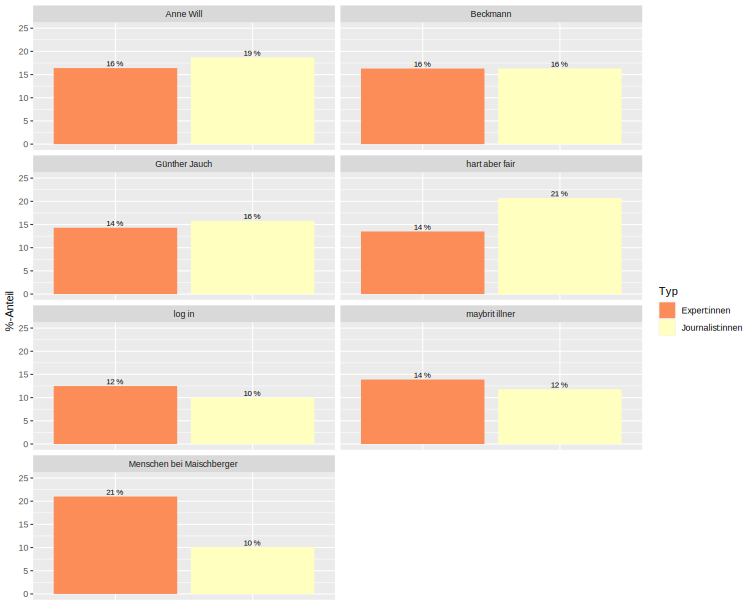
\includegraphics[width=1\textwidth]{daten/grafiken/plot_journalisten_experten.png}
	%Captions and Labels can be used since this is a figure environment
	\caption{Anteil von Journalisten und Experten nach Sendungen}
	\label{plot:journalisten_experten}
\end{figure}

In den einzelnen Sendungen ergibt sich ein ähnliches Bild wie in der Gesamtschau, allerdings zeigen sich auch hier einige Besonderheiten: Plasberg setzt stärker als alle anderen Sendungen auf die Diskussion mit seinen Berufskollegen und lädt dafür etwas weniger Experten ein. Bei Beckmann werden beide Gruppen eher selten eingeladen, genauso wie bei \textit{log in}. Hingegen setzt Maischberger stärker auf Experten, denn auf Journalisten. Es kann bei dieser Sendung also keine Rede von einem angeblich „starken Hang zur Kollegenorientierung“ \parencite{hachmeisterARDNurKeine2011} sein.

Schlüsselt man die Expertengruppe weiter auf (vgl. Tabelle \vref{tab:verteilung_experten}), so wird deutlich, dass dies bei Beckmann  und Maischberger am häufigsten Ärzte sind. Dies ist insofern logisch, als beide Sendungen relativ oft Gesundheitsthemen behandeln (vgl. Kapitel \vref{chap:themenbereiche} ). In den anderen Sendungen dominieren dagegen Wissenschaftler (\textit{Anne Will, Günther Jauch, log in, maybrit illner}). Wiederum wird daran der seriöse Anspruch der Sendungen deutlich. Einzig bei \textit{hart aber fair} stehen „sonstige Experten“ auf Platz eins, dies umfasst Politik- und Kommunikationsberater ebenso wie Personen die beispielsweise als Finanz- oder Nahostexperten vorgestellt werden ohne Hinweis auf eine eventuell universitäre oder wissenschaftliche Tätigkeit\footnote{Der Expertenstatus kann dabei durchaus zweifelhaft sein. So trat zum Beispiel allein Gertrud Höhler im Untersuchungszeitraum siebenmal auf. Vorgestellt wurde sie  meist als Politikberaterin (vgl. \textit{hart aber fair} vom 12.12.2011, \textit{Anne Will} vom 14.03. und 16.05.2012, \textit{Günther Jauch} vom 26.08.2012). Dabei gibt es allerdings erhebliche Zweifel daran, dass sie jemals als Politikberaterin tätig war \parencite{langguthLegendeKanzlerberaterin2012}. Sie selbst konnte – ironischerweise in der Talkshow \textit{Markus Lanz} – nicht erklären, wen sie beraten habe \parencite{sasseGertrudHoehlerDemontiert2012}. Den Redaktionen von \textit{Anne Will}, \textit{hart aber fair}, \textit{Günther Jauch} und \textit{Menschen bei Maischberger} kamen solche Zweifel allerdings offenbar nicht.}.

\begin{table}[ht]
	\centering
	\caption{Verteilung innerhalb der Gruppe „Experten“ (alle Sendungen)}
	\resizebox{\textwidth}{!}{%
		\begin{tabular}{@{}ccccc@{}}
			\toprule
			\textbf{} & \textbf{Wissenschaft} & \textbf{Rechtsanwälte / Juristen} & \textbf{Ärzte} & \textbf{Sonstige Experten} \\ \midrule
			\begin{tabular}[c]{@{}c@{}}Anne Will\\ (n=35)\end{tabular}       & 51,40 \% & 5,70 \%  & 20,00 \% & 22,90 \% \\
			\begin{tabular}[c]{@{}c@{}}Beckmann\\ (n=32)\end{tabular}        & 31,30 \% & 6,30 \%  & 37,50 \% & 25,00 \% \\
			\begin{tabular}[c]{@{}c@{}}Günther Jauch\\ (n=29)\end{tabular}   & 48,30 \% & 13,80 \% & 0,00 \%  & 37,90 \% \\
			\begin{tabular}[c]{@{}c@{}}hart aber fair\\ (n=26)\end{tabular}  & 30,80 \% & 11,50 \% & 15,40 \% & 42,30 \% \\
			\begin{tabular}[c]{@{}c@{}}log in\\ (n=20)\end{tabular}          & 65,00 \% & 5,00 \%  & 10,00 \% & 20,00 \% \\
			\begin{tabular}[c]{@{}c@{}}maybrit illner\\ (n=33)\end{tabular}  & 48,50 \% & 3,00 \%  & 21,20 \% & 27,30 \% \\ \midrule
			\begin{tabular}[c]{@{}c@{}}Maischberger\\ (n=50)\end{tabular}    & 28,00 \% & 4,00 \%  & 40,00 \% & 28,00 \% \\
			\begin{tabular}[c]{@{}c@{}}Alle Sendungen\\ (n=225)\end{tabular} & 41,30 \% & 6,70 \%  & 23,10 \% & 28,90 \% \\ \bottomrule
		\end{tabular}%
	}
	\label{tab:verteilung_experten}
\end{table}

\subsubsection{Zivilgesellschaft}

Vertreter der Zivilgesellschaft, also von Verbänden, Initiativen oder sozialen Bewegungen könnten ein Gegengewicht zur partei- bzw. wirtschaftsnahen Gästeauswahl bieten. Allerdings wurde bereits dargestellt, dass recht selten Gäste aus diesem Bereich eingeladen werden und ihr Anteil so insgesamt nur bei 5,3 \% liegt. Die einzige Ausnahme bildet hier \textit{log in} mit 15 \%, womit sich die Sendung von den etablierten Polittalks unterscheidet und eine größere Offenheit gegenüber außerparlamentarischen Bewegungen zeigt.

Unterteilt man die Kategorie nochmals in drei Untergruppen – \textit{Sozialverbände}, \textit{NGOs / Vereine / Soziale Bewegungen} und \textit{sonstige Zivilgesellschaft} – so zeigt sich, dass Vertreter der großen Sozialverbände, also beispielsweise der Caritas oder des Sozialverbands VDK Deutschland, den kleinsten Teil der Gruppe ausmachen (vgl. Tabelle \vref{tab:zivilgesellschaft}). Dies ist erstaunlich, als es sich ja durchaus anbieten würde zu Themen der Sozialpolitik diese einzuladen. Den größten Teil der Gruppe machen stattdessen Vertreter von Nichtregierungsorganisationen, Vereinen und Sozialen Bewegungen aus. Das Spektrum ist dabei recht groß und reicht von Attac, über Occupy bis zu Greenpeace. Daneben gibt es noch eine dritte Untergruppe, die der sonstigen Zivilgesellschaft, die den zweitgrößten Anteil innerhalb der Kategorie hat und zu der Personen zählen, die in den Talkshows zwar als Aktivist vorgestellt wurden, allerdings ohne, dass eine Organisationszugehörigkeit thematisiert wurde.

\begin{table}[ht]
	\centering
	\caption{Verteilung innerhalb der Gruppe „Zivilgesellschaft“ (alle Sendungen)}
	\resizebox{\textwidth}{!}{%
		\begin{tabular}{@{}cccc@{}}
			\toprule
			& \textbf{Sozialverbände} & \textbf{\begin{tabular}[c]{@{}c@{}}NGOs / Vereine /\\ Soziale Bewegungen\end{tabular}} & \textbf{Sonstige Zivilgesellschaft} \\ \midrule
			\textbf{\begin{tabular}[c]{@{}c@{}}Anne Will\\ (n=8)\end{tabular}}       & 37,50 \% & 12,50 \%  & 50,00 \%  \\
			\textbf{\begin{tabular}[c]{@{}c@{}}Beckmann\\ (n=3)\end{tabular}}        & 0,00 \%  & 100,00 \% & 0,00 \%   \\
			\textbf{\begin{tabular}[c]{@{}c@{}}Günther Jauch\\ (n=3)\end{tabular}}   & 0,00 \%  & 0,00 \%   & 100,00 \% \\
			\textbf{\begin{tabular}[c]{@{}c@{}}hart aber fair\\ (n=12)\end{tabular}} & 0,00 \%  & 75,00 \%  & 25,00 \%  \\
			\textbf{\begin{tabular}[c]{@{}c@{}}Maischberger\\ (n=9)\end{tabular}}    & 11,10 \% & 55,60 \%  & 33,30 \%  \\
			\textbf{\begin{tabular}[c]{@{}c@{}}log in\\ (n=24)\end{tabular}}         & 4,20 \%  & 79,20 \%  & 16,70 \%  \\
			\textbf{\begin{tabular}[c]{@{}c@{}}maybrit illner\\ (n=17)\end{tabular}} & 0,00 \%  & 88,20 \%  & 11,80 \%  \\ \midrule
			\textbf{\begin{tabular}[c]{@{}c@{}}ARD-Talks\\ (n=35)\end{tabular}}      & 11,40 \% & 51,40 \%  & 37,20 \%  \\
			\textbf{\begin{tabular}[c]{@{}c@{}}Alle Sendungen\\ (n=76)\end{tabular}} & 6,60 \%  & 68,40 \%  & 25,00 \%  \\ \bottomrule
		\end{tabular}%
	}
	\label{tab:zivilgesellschaft}
\end{table}

Bemerkenswert ist darüber hinaus, dass bei \textit{Günther Jauch} insgesamt nur drei Vertreter der Zivilgesellschaft  zu Wort kamen und es sich hierbei zudem um Personen handelt, die als eigenständig tätige Aktivist vorgestellt wurden. Wenn man berücksichtigt, dass bei \textit{Günther Jauch} zudem kein Gewerkschafter auftrat, wird deutlich, dass sich die Sendung durch ihre Gästepolitik konsequent von außerparlamentarisch organisierten Interessen abschottet – außer solchen der Wirtschaft versteht sich.

Es muss also festgehalten werden, dass sich nach Unterteilung der Gäste in verschiedenen Rollengruppen eine Dominanz wirtschaftsnaher Vertreter im Vergleich zu arbeitnehmernahen sowie bundespolitischer Akteure gegenüber Politiker aus anderen Bereichen zeigt.

\subsection{Parteizugehörigkeit}\label{chap:parteizugehoerigkeit}

Um Ungleichheiten bei der Einladung von Politiker festzustellen, wurde die Verteilung innerhalb der einzelnen Sendungen mit den Ergebnissen der letzten Bundestagswahl verglichen. Da diese bereits 2009 stattfanden, also drei Jahre vor den untersuchten Talkshows und in der Zwischenzeit einige Veränderungen in der bundesdeutschen Parteienlandschaft festzustellen waren\footnote{Im Erhebungszeitraum verpasste unter anderem die FDP den Wiedereinzug in die Parlamente in Mecklenburg-Vorpommern \parencite{dielandeswahlleiterinEndgultigesErgebnisLandtagswahlo.J.}, Berlin \parencite{dielandeswahlleiterinZweitstimmenBeiWahlo.J.} und dem Saarland \parencite{dielandeswahlleiterinEndgultigesAmtlichesEndergebniso.J.}. Gleichzeitig gelang der Piratenpartei bei diesen Wahlen erstmalig der Einzug in die Parlamente in Berlin \parencite{dielandeswahlleiterinZweitstimmenBeiWahlo.J.}, dem Saarland \parencite{dielandeswahlleiterinEndgultigesAmtlichesEndergebniso.J.} und NRW \parencite{dielandeswahlleiterinEndgultigesErgebnisFuro.J.}, damit konnte sie sich im Parteienspektrum etablieren.}, muss die Aussagekraft dieses Vergleichs allerdings eingeschränkt werden.

\subsubsection{Alle Sendungen}

Es lässt sich festhalten, dass im Großen und Ganzen in allen Sendungen der Proporz zwischen den Parteien mehr oder weniger gewahrt wird. Ein Befund der schon für \textit{Sabine Christiansen} galt \parencite[6]{muellerSchaubuehneFuerEinflussreichen2006}. Die Abweichungen zum Bundestagsergebnis bleiben meist unterhalb von fünf Prozent (vgl. Abbildungen \vref{plot:parteizugehoerigkeit} \& \vref{tab:parteizugehoerigkeit}).

\begin{figure}[ht]
	%Do not try to scale figure in .tex or you loose font size consistency
	\centering
	%The code to input the plot is extremely simple
	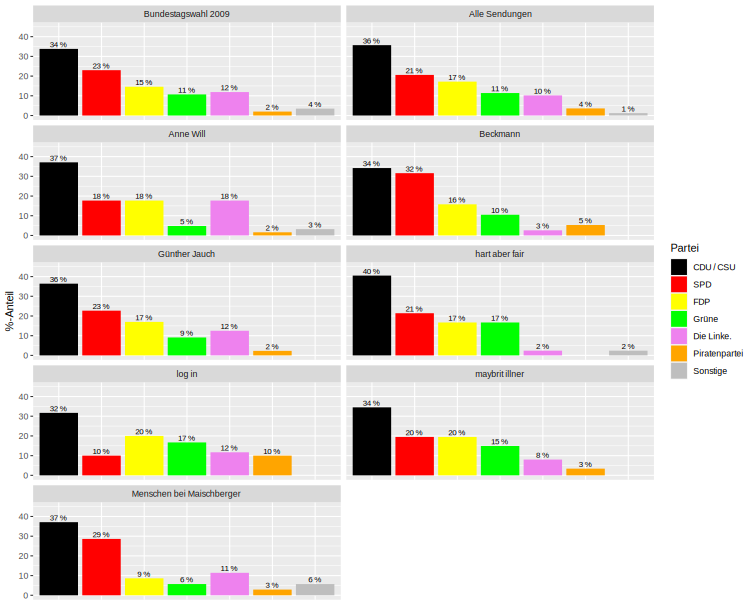
\includegraphics[width=1\textwidth]{daten/grafiken/plot_parteizugehoerigkeit.png}
	%Captions and Labels can be used since this is a figure environment
	\caption{Vergleich Parteienzugehörigkeit mit Bundestagswahl}
	\subcaption*{(vgl. auch ausführliche Tabelle \vref{tab:anhang_parteizugehoerigkeit_sendungen} im Anhang)}
	\label{plot:parteizugehoerigkeit}
\end{figure}

Dennoch zeigen sich bei einigen Sendungen bemerkenswerte Abweichungen. Die CDU / CSU ist in allen Sendungen außer \textit{log in} überrepräsentiert, wenn auch meist in einem relativ kleinen Rahmen. Einzig bei \textit{hart aber fair} beträgt die Abweichung +6,7 \% gegenüber ihrem Ergebnis bei der Bundestagswahl.

Ebenfalls meist häufiger eingeladen waren FDP-Vetreter. Hier liegt die Abweichung zwar auch bis auf zwei Fälle unter fünf Prozent, dennoch ist dies insofern erstaunlich, als die FDP im Untersuchungszeitraum in Umfragen fast konstant unter 5 \% lag, also weit unter ihrem Ergebnis von 2009 (14,6 \%) und zudem bei drei Landtagswahlen nicht wieder in die jeweiligen Parlamente gewählt wurde. Die beiden größten Abweichungen hinsichtlich der FDP gibt es bei \textit{Maischberger}, wo sie 8,6 \% der Politikerauftritte mit ihren Vertreter besetzen konnten und log in, wo sie wiederum auf fast 20 \% kamen. Da wir nicht in die Abläufe der Redaktionen hineinblicken können, kann es sowohl sein, dass die FDP bei beiden Sendungen bewusst seltener bzw. häufiger eingeladen wurde als auch, dass FDP-Politiker sich bewusst gegen bzw. für die Teilnahme in den beiden Formaten entschieden haben. Nichtsdestotrotz handelt es sich dabei um eine  Verletzung des Ausgewogenheitsgebots.

SPD-Politiker sind hingegen bei \textit{Beckmann} relativ häufiger zu Gast (+8,6 \% im Vergleich zu ihrem Bundestagsergebnis), worunter wiederum die Präsenz der Linkspartei leidet (-9,3 \%).

\begin{table}[ht]
	\centering
	\resizebox{\textwidth}{!}{%
		\begin{tabular}{@{}cccccccc@{}}
			\toprule
			\textbf{} & \textbf{CDU / CSU} & \textbf{FDP} & \textbf{SPD} & \textbf{Grüne} & \textbf{Linkspartei} & \textbf{Piratenpartei} & \textbf{Sonstige} \\ \midrule
			\textbf{Anne Will }     & 3,30 \%          & 3,10 \%           & \textbf{-5,30 \%}  & \textbf{-5,90 \%} & \textbf{5,80 \%}  & -0,40 \%         & -0,30 \% \\
			\textbf{Beckmann}       & 0,40 \%          & 1,20 \%           & \textbf{8,60 \%}   & -0,20 \%          & \textbf{-9,30 \%} & 3,30 \%          & -3,50 \% \\
			\textbf{Günther Jauch}   & 2,60 \%   & 2,40 \% & -0,30 \% & -1,60 \% & 0,60 \%     & 0,30 \%       & -3,50 \% \\
			\textbf{hart aber fair} & \textbf{6,70 \%} & 2,10 \%           & -1,60 \%           & \textbf{6,00 \%}  & \textbf{-9,50 \%} & -2,00 \%         & -1,10 \% \\
			\textbf{Maischberger}   & 3,30 \%          & \textbf{-6,00 \%} & \textbf{5,60 \%}   & \textbf{-5,00 \%} & -0,50 \%          & 0,90 \%          & 1,70 \%  \\
			\textbf{log in}         & -2,10 \%         & \textbf{5,40 \%}  & \textbf{-13,00 \%} & \textbf{6,00 \%}  & -0,20 \%          & \textbf{8,00 \%} & -3,50 \% \\
			\textbf{maybrit illner}  & 0,70 \%   & 4,90 \% & -3,50 \% & 4,20 \%  & -3,90 \%    & 1,40 \%       & -3,50 \% \\ \midrule
			\textbf{ARD-Talkschiene} & 3,20 \%   & 1,20 \% & 0,30 \%  & -1,60 \% & -1,30 \%    & 0,30 \%       & -2,10 \% \\
			\textbf{Alle Sendungen}  & 1,90 \%   & 2,60 \% & -2,40 \% & 0,70 \%  & -1,70 \%    & 1,60 \%       & -2,30 \% \\ \bottomrule
		\end{tabular}%
	}
	\caption{Parteizugehörigkeit im Vergleich zum Bundestagswahlergebnis 2009}
	\subcaption*{Abweichungen über 5\% sind hervorgehoben}
	\label{tab:parteizugehoerigkeit}
\end{table}

Wenn nicht zwischen den einzelnen Parteien differenziert wird, sondern zwischen Bundesregierung und Opposition, dann verdeutlicht Abbildung \vref{plot:parteizugehoerigkeit}, dass die Regierungsparteien in fast allen Sendungen, bis auf \textit{Beckmann} und \textit{Maischberger}, im Vergleich zur Opposition überrepräsentiert sind. Besonders deutlich ist dies bei \textit{hart aber fair}, wo CDU/CSU und FDP zusammen auf gut 57 \% aller Politikerauftritte kommen, dort ist zudem die Linkspartei deutlich unterrepräsentiert – faktisch kommt sie kaum vor, genauso wie die Piratenpartei. Damit wird die Beobachtung bestätigt, dass die Regierungsparteien medial überproportional oft vorkommen \parencites{amendtSchwarzgelberKanalDeutsche2012}[144]{hoffmannPolitischeFernsehinterviewsEmpirische1982}.

Beachtenswert ist zudem, dass im Grunde nur die etablierten Parteien eingeladen werden. Neben der großen Ausnahme Piratenpartei, die aufgrund ihrer damaligen Wahlerfolge schlechterdings nicht vollständig ignoriert werden konnte, kommen bloß zwei Vertreter der Freien Wähler und zweimal Jutta Ditfurth von der Kleinstpartei Ökologische Linke vor. Der Ausschluss sowohl links- als auch rechtsradikaler Parteien und Gruppierungen funktioniert hier also weiterhin.

\subsubsection{Sendungen zum Thema Eurokrise}

Ein wenig anders sieht die Verteilung allerdings bei den Sendungen zur Eurokrise aus. Wie aus Abbildung \vref{plot:parteizugehoerigkeit_euro} ersichtlich, kann man zwei Gruppen bilden. Auf der einen Seite die Sendungen in denen CDU / CSU und FDP überrepräsentiert sind und auf der der anderen diejenigen in denen Oppositionsparteien überrepräsentiert sind.

\begin{figure}[ht]
	%Do not try to scale figure in .tex or you loose font size consistency
	\centering
	%The code to input the plot is extremely simple
	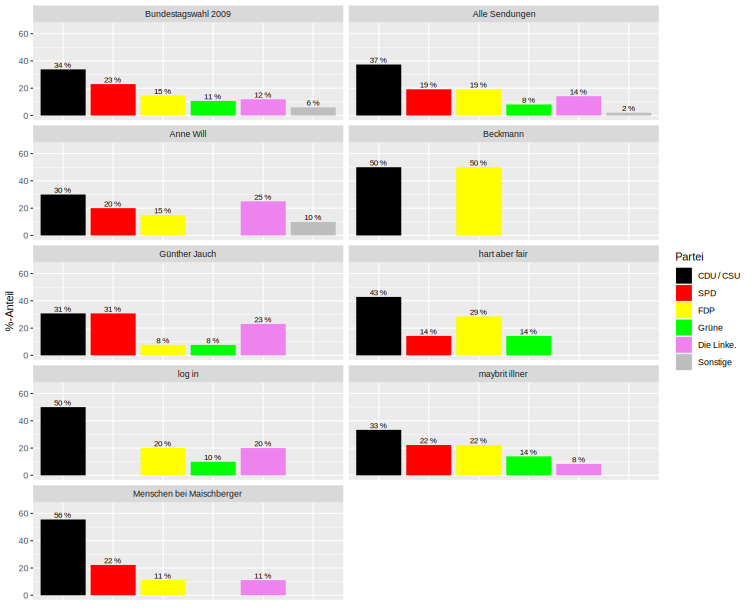
\includegraphics[width=1\textwidth]{daten/grafiken/plot_parteizugehoerigkeit_euro.png}
	%Captions and Labels can be used since this is a figure environment
	\caption{Vergleich Parteienzugehörigkeit mit Bundestagswahl (Sendungen zum Thema Eurokrise)}
	\label{plot:parteizugehoerigkeit_euro}
\end{figure}

Zur ersten Gruppe gehören \textit{Beckmann}, \textit{hart aber fair}, \textit{Menschen bei Maischberger}, \textit{log in} und \textit{maybrit illner}. Besonders eklatant sind die Werte bei \textit{Beckmann}, wo nur Politiker der Regierungsparteien eingeladen waren. Dem gegenüber stehen bloß zwei Sendungen, in denen die Oppositionsparteien häufiger vertreten sind als die Regierungsparteien – \textit{Anne Will} und \textit{Günther Jauch}. Der Regierung fällt es damit wesentlich leichter ihre Positionen zur Eurokrise in den Sendungen unterzubringen als der Opposition.

Parteispezifisch sind zudem die relativ hohen Werte der Linkspartei bei \textit{Anne Will}, \textit{Günther Jauch} und \textit{log in} erwähnenswert. Dafür fehlt die Partei bei \textit{hart aber fair} komplett. Nimmt man alle Sendungen zusammen führt dies dazu, dass die Werte fast dem Ergebnis der letzten Bundestagswahl entsprechen, was auch zeigt, dass gerade die kleineren Parteien vornehmlich zu ihren „Spezialthemen“ eingeladen werden.

\subsection{Demografie}\label{chap:demografie}

Zum Abschluss sollen hier noch die beiden erhobenen demografischen Merkmale – Alter und Geschlecht – näher betrachtet werden.

\subsubsection{Altersstruktur}

Hinsichtlich der Altersstruktur kann bei fast allen Sendungen festgestellt werden, dass das jeweilige Gästepanel im Vergleich zum Bevölkerungsdurchschnitt überaltert ist. Einzig \textit{log in} bewegt sich mit einem Altersdurchschnitt von 45 Jahren relativ nahe am Durchschnittsalter der Bevölkerung von 43,7 Jahren und unterstreicht damit leidlich seine Ausrichtung als „junges“ Format auf ein jüngeres Publikum.

\begin{table}[ht]
	\centering
	\caption{Altersstruktur der Talkshows}
	%\resizebox{\textwidth}{!}{%
		\begin{tabular}{@{}ccccl@{}}
			\toprule
			& \textbf{Median} & \textbf{Min} & \textbf{Max} & \textbf{N}         \\ \midrule
			\textbf{Anne Will}      & 57              & 21           & 92           & 210 (fehlend 4)    \\
			\textbf{Beckmann}       & 51              & 18           & 94           & 156 (fehlend 40)   \\
			\textbf{Günther Jauch} & 57              & 14           & 93           & 189 (fehlend 14)   \\
			\textbf{hart aber fair} & 52              & 18           & 81           & 184 (fehlend 9)    \\
			\textbf{Maischberger}   & 58              & 15           & 94           & 205 (fehlend 33)   \\
			\textbf{log in}         & 45              & 18           & 82           & 143 (fehlend 17)   \\
			\textbf{maybrit illner} & 56              & 20           & 88           & 219 (fehlend 18)   \\ \midrule
			\textbf{ARD-Talks}      & 56              & 14           & 94           & 1087 (fehlend 100) \\
			\textbf{Alle Sendungen} & 54              & 14           & 94           & 1306 (fehlend 134) \\ \bottomrule
		\end{tabular}%
	%}
	\label{tab:altersstruktur}
\end{table}

Die „älteste“ Sendung ist \textit{Menschen bei Maischberger}, wo die Gäste im Schnitt fast 58 Jahre alt sind, dicht gefolgt von\textit{ Günther Jauch} mit circa 56 Jahren. Der „jüngste“ ARD-Polittalk ist hart aber fair mit einem Durchschnitt von knapp 53 Jahren. Insgesamt sind die Unterschiede zwischen den sechs etablierten Talks aber vernachlässigbar (vgl. Tabelle \vref{tab:altersstruktur}).

Die Problematik dieser Überalterung zeigt sich noch deutlicher, wenn man sich vor Augen führt, dass nur 3,7 \% der Gäste unter 30 Jahre alt waren, während die Altersgruppe der 40 bis 69jährigen 61,5 \% der Gäste und selbst die über 80jährigen noch 4,5 \% ausmachten. Die jüngeren Generationen selbst – und damit wahrscheinlich auch ihre politischen Meinungen und Ansichten – kommen folglich kaum vor in den Sendungen.

Da das Phänomen in sechs der sieben Talks auftritt, kann es auch nur bedingt über eine bestimmte Zielgruppenausrichtung erklärt werden. Zwar könnte man durchaus den hohen Altersschnitt bei \textit{Menschen bei Maischberger} mit einer gezielten Ansprache eines ebenfalls älteren Publikums erklären – und rechtfertigen. Die gleiche Begründung kann aber etwa bei \textit{Günther Jauch} oder \textit{maybrit illner} nicht angewendet werden, richten sich diese Sendungen doch ihrem Anspruch nach an die gesamte Bevölkerung.

Allerdings kann die Altersstruktur vielleicht erklären, warum die Konsumenten von Polittalks, zumindest vor zehn Jahren, mit einem Schnitt von 62 bis 64 Jahren ein noch höheres Alter aufwiesen \parencite[309f.]{gerhardsTalkshownutzungUndTalkshownutzer2002}.

\subsubsection{Geschlechterverhältnis}

Ein ähnlich ernüchterndes Bild wie bei der Altersstruktur ergibt ein Blick auf das Geschlechterverhältnis der eingeladenen Gäste.

\begin{figure}[ht]
	%Do not try to scale figure in .tex or you loose font size consistency
	\centering
	%The code to input the plot is extremely simple
	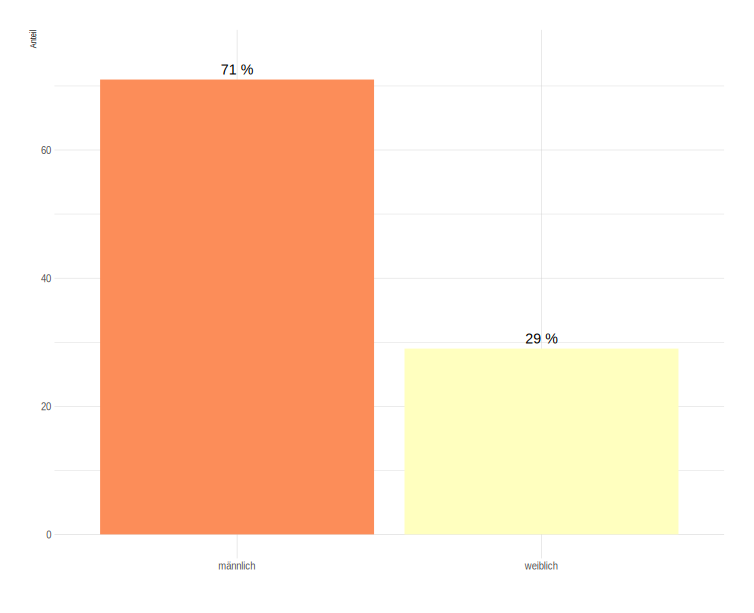
\includegraphics[width=1\textwidth]{daten/grafiken/plot_geschlechterverhaeltnis_gesamt.png}
	%Captions and Labels can be used since this is a figure environment
	\caption{Geschlechterverhältnis der Gäste}
	\subcaption*{alle Sendungen; n = 1441}
	\label{plot:geschlechterverhaeltnis_gesamt}
\end{figure}

Wie aus der obigen Abbildung ersichtlich wird, dominieren unter den Gästen Männer mit über 70 \%. Hält man sich vor Augen, dass in Deutschland das Verhältnis zwischen Männern und Frauen bei 51 \% zu 49 \% liegt \parencite{statistischesbundesamtBevoelkerungsstand2011}, so wird klar, dass die untersuchten Sendungen hier eklatant gesellschaftliche Ungleichheit reproduzieren\footnote{Solche Ungleichheiten zeigen sich etwa in der weiterhin schlechteren Bezahlung von Frauen oder dem ungleichen Zugang zu Führungspositionen in Politik und Wirtschaft \parencite{hausmannGlobalGenderGap2012}}.

Die Tendenz ist dabei bei alle Talksendungen gleich (vgl. Abbildung \vref{plot:geschlechterverhaeltnis_sendungen}), auffallend sind einzig die beiden ZDF-Talks, da bei ihnen das Verhältnis noch ungünstiger ist, und die beiden „weicheren“ ARD-Formate \textit{Beckmann} und \textit{Menschen bei Maischberger}, bei denen das Verhältnis ein wenig ausgeglichener ist.

\begin{figure}[ht]
	%Do not try to scale figure in .tex or you loose font size consistency
	\centering
	%The code to input the plot is extremely simple
	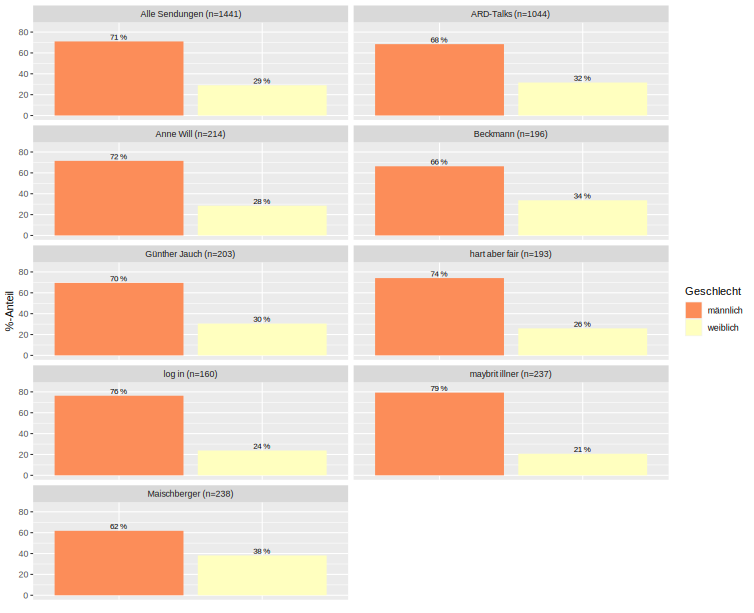
\includegraphics[width=1\textwidth]{daten/grafiken/plot_geschlechterverhaeltnis_sendungen.png}
	%Captions and Labels can be used since this is a figure environment
	\caption{Geschlechterverhältnis der Gäste nach Sendungen}
	\label{plot:geschlechterverhaeltnis_sendungen}
\end{figure}

Wird das Geschlechterverhältnis nach Themenbereichen aufgeschlüsselt, so kann man feststellen, dass in Sendungen zu Kriminalität und Katastrophen, zu Prominenz oder Gesundheit sowie bei sonstigen Themen, der Anteil weiblicher Gäste deutlich größer ist als bei Themen aus den Bereichen Politik, Wirtschaft oder auch Sport (vgl. Abbildung \vref{plot:geschlechterverhaeltnis_themen}).

\begin{figure}[ht]
	%Do not try to scale figure in .tex or you loose font size consistency
	\centering
	%The code to input the plot is extremely simple
	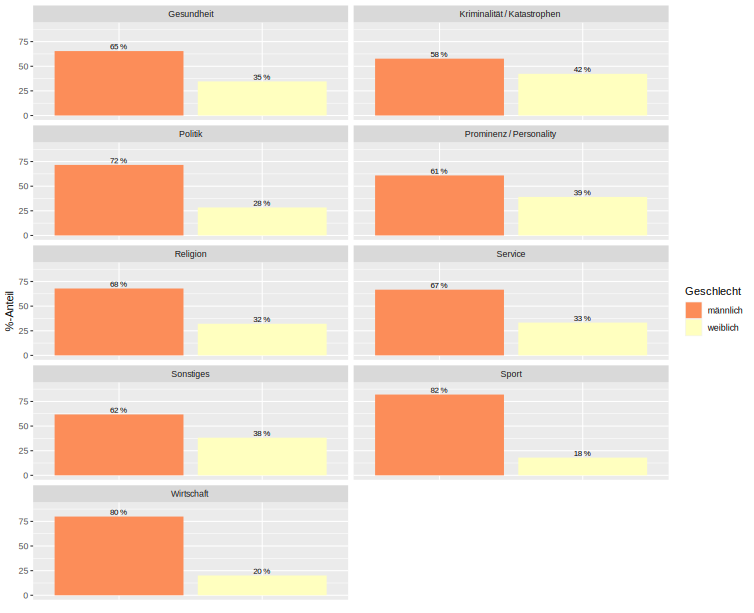
\includegraphics[width=1\textwidth]{daten/grafiken/plot_geschlechterverhaeltnis_themen.png}
	%Captions and Labels can be used since this is a figure environment
	\caption{Geschlechterverhältnis der Gäste nach Themenbereichen}
	\label{plot:geschlechterverhaeltnis_themen}
\end{figure}

Es scheint also so, als ob die Redaktionen bei unpolitischeren, boulevardesken Themen eher Frauen einladen als bei den seriösen Themen. Damit reproduzieren die Sendungen gesellschaftliche Ungleichheiten. So liegt der Frauenanteil im Bundestag beispielsweise  nur bei knapp 33 \% (Deutscher Bundestag 2011) und Führungspositionen in der Wirtschaft werden ebenfalls nur zu 30 \% von Frauen besetzt \parencite{hostFuhrungskrafteMonitor20122012}.

Wenn man bedenkt, dass Medien nicht bloß die Realität widerspiegeln, sondern sie mit schaffen und beeinflussen, ist es nicht einzusehen, warum politische Talkshows existierende soziale Ungleichheiten bloß reproduzieren, anstatt versuchen diese auszugleichen. Zumal die öffentlich-rechtlichen Sender in den entsprechenden Gesetzen zur Förderung der Gleichstellung verpflichtet sind (vgl. Kapitel \vref{chap:anforderungen}). Zumal sich hier ein Zustand vorsetzt, der bereits an \textit{Sabine Christiansen} kritisiert wurde, deren Frauenanteil allerdings noch bei nur 12 \% lag \parencite[3]{muellerSchaubuehneFuerEinflussreichen2006}.

\section{Zwischenfazit}

Die Untersuchung der Themenstruktur ergab, dass sich die Sendung anhand der abgedeckten Themenbereiche in zwei Gruppen einteilen lassen. Zum einen die reinen Polittalks, die sich überwiegend mit rein politischen Themen befassen und zum anderen die in Richtung Personality-Show tendierenden Formate, die einen bunteren Themenmix bieten der auch unpolitische Themen enthält. Zur ersten Gruppe gehören \textit{Anne Will}, \textit{Günther Jauch}, \textit{log in} und \textit{maybrit illner}, zur zweiten Beckmann, \textit{Menschen bei Maischberger} und – erstaunlicherweise – \textit{hart aber fair}.

Unter den politischen Themen dominiert bei allen Sendungen die Innenpolitik klar. Daneben spielen nur noch sozialpolitische Themen eine nennenswerte Rolle. Alle erfassten Politikbereiche kommen einzig bei \textit{Günther Jauch} vor. log in kennzeichnet ein relativ hoher Anteil umweltpolitischer Thematiken.

Doppelungen, bei denen verschiedene Sendungen das gleiche Thema in kurzer Zeit behandeln, lassen sich immer wieder finden. Insbesondere bei aktuellen „Aufregerthemen“ wie der Wulff-Affäre ist dies der Fall, aber auch bei zeitlosen Thematiken wie dem Burnout-Syndrom. Hinzukommt, dass sich die Titel vieler Talkfolgen durch einen alarmistischen Grundton und einseitige Vorfestlegungen statt neutraler Formulierungen auszeichnen.

Resümierend lässt sich festhalten, dass der ARD-Programmausschuss mit folgender Ein"-schätz"-ung der hauseigenen Talkschiene weitgehend richtig liegt:

\begin{quote}
	„Alle-fünf (sic!) Talk-Sendungen sind unpolitischer geworden, was dazu führt, dass wichtige, gesellschaftlich relevante Themen, die komplex und somit er"-klärungs"-be"-dürf"-tig sind, nicht behandelt werden. Nach wie vor fehlen wirtschaftspolitische Themen sowie unterschiedliche Themen der Sozial- und Energiepolitik fast völlig, ebenso wie neue politische Bewegungen und die Internationale Politik. Auch die Wirtschafts- und Finanzmarktkrise in Europa wird nicht adäquat und genügend differenziert behandelt, Hinzu (sic!) kommt, dass es nach wie vor Themendoppelungen gibt (z. B. Essen, Gesundheit), dio (sic!) nicht notwendig sind.“ \parencite{harbuschGeheimPapierARDKritisiert2012}
\end{quote}

Allerdings kann man diese Diagnose aufgrund der hier vorliegenden Daten zugleich einschränken als auch erweitern. Von einer Häufung unpolitischer Themen kann im Grunde nur bei hart aber fair gesprochen werden. Sowohl \textit{Anne Will} als auch \textit{Günther Jauch} haben einen hohen Anteil an politischen Themen im engeren Sinne und \textit{Beckmann} bzw. \textit{Menschen bei Maischberger} dürften aufgrund ihrer Nähe zu Personality-Talks bereits mehr unpolitische Themen geboten haben. Auch ob die Finanz- und Eurokrise nicht ausreichend berücksichtigt wurde, ist zumindest Interpretationssache, wurde das Thema doch innerhalb eines Jahres immerhin 24-mal von den ARD-Talks behandelt (vgl. Tabelle \vref{tab:themencluster}) – ob sie hingegen differenziert genug behandelt wurde, wird die folgende qualitative Sendungsanalyse zeigen. Auszuweiten ist die Diagnose hingegen insofern, als dass sie nicht nur auf die ARD-Talkschiene zutrifft, sondern ebenso auf die beiden untersuchten Polittalks des ZDF – auch bei diesen werden viele politische Themenfelder vernachlässigt und es kommt zu Themendoppelungen mit den anderen öffentlich-rechtlichen Talks. Diese Einseitigkeiten schränken sowohl Pluralität als auch Relevanz der Sendungen ein.

Hinsichtlich der Gästestruktur lässt sich resümieren, dass der Anteil von Politikern je nach Thema und Sendung relativ hoch ist. Dies gilt vor allem für die jeweiligen Talkflaggschiffe \textit{Günther Jauch} und \textit{maybrit illner}. Gleichzeitig ist die Dominanz allerdings nicht mehr ganz so stark ausgeprägt wie noch 1999, als über zwei Drittel der Gäste bei \textit{Sabine Christiansen} Politiker waren \parencite[141]{doernerPolitainmentPolitikMedialen2001}.

Allerdings zeichnet sich die Gruppe der Politiker durch eine hohe Zahl an mehreren Auftritten der gleichen Personen aus. Dies ist bei den anderen Gästegruppen im Allgemeinen nicht in derartigem Ausmaß der Fall, somit kann von einer talkenden Politikerelite gesprochen werden. Speziell beim Thema Eurokrise lässt sich allerdings ein Absinken des Wiederholungsquotienten bei Politiker und ein Anstieg bei Experten und Wirtschaftsvertretern feststellen. Hier ist also eher von einer Elite von Personen aus den drei Gruppen zu sprechen.

Die Gruppe der Politiker zeichnet sich darüber hinaus durch ein Übergewicht von Bundespolitikern aus. Bei der Parteizugehörigkeit zeigt sich hingegen der Versuch den Proporz zu wahren. Dies gelingt mehr oder weniger gut, allerdings gibt es bei sechs der sieben Sendungen eine Übervorteilung der Regierungsparteien im Vergleich zum Ergebnis der letzten Bundestagswahl. Am größten ist diese Verzerrung bei \textit{hart aber fair}. \textit{log in} sticht hingegen durch eine häufige Einladung von Vertretern der Piratenpartei hervor. Bei den Talks, welche die Eurokrise behandeln, ist die Überrepräsentation der Regierungsparteien nochmals um ein gutes Stück größer. Hier ist \textit{Beckmann} der Extremfall, wo keinerlei Oppositionspolitiker zu Wort kommen. Die Verzerrung bei \textit{maybrit illner} ist allerdings aufgrund der höheren Anzahl an politischen Gästen und Folgen zur Eurokrise aufs Ganze betrachtet problematischer.

Im Bereich der Wirtschaftsvertreter zeigt sich eine eklatante Verzerrung zu Gunsten von wirtschaftsnahen Personen, die bei den Folgen zur Eurokrise nochmals stärker ist. Ähnliches gilt für Vertreter der Zivilgesellschaft, die nur in geringem Umfang in den Sendungen zu Wort kamen – mit Ausnahme von \textit{log in} – und damit nicht die Dominanz der Wirtschaft ausgleichen können, zumal die klassischen Sozialverbände nur noch selten eingeladen werden. Hiermit setzt sich eine Diagnose fort, die bereits in gleicher Weise für \textit{Sabine Christiansen} galt \parencite[7]{muellerSchaubuehneFuerEinflussreichen2006}. Bei Journalisten und Experten gibt es keine ungewöhnlichen Auffälligkeiten. \textit{Beckmann} und \textit{Menschen bei Maischberger} setzten entsprechend ihrer thematischen Ausrichtung stark auf Ärzt, \textit{hart aber fair} auf sonstige Experten und die restlichen Talks auf Wissenschaftler.

Ebenfalls große Abweichungen zeigen die beiden demografischen Indikatoren. Sowohl was das Alter der Gäste als auch ihr Geschlecht an geht, weichen die Sendungen stark vom gesellschaftlichen Durchschnitt ab. Das Format mit den jüngsten Gästen ist wenig überraschend log in. Beim Geschlechterverhältnis sind \textit{Beckmann} und \textit{Menschen bei Maischberger} am nächsten an der realen Verteilung, allerdings nur weil zu unpolitischen Themen tendenziell mehr Frauen eingeladen werden als zu politischen.

Die Talkshows insgesamt reproduzieren also gesellschaftliche Ungleichheiten – sei es die Benachteiligung von Frauen, die Überalterung politischer Debatten, die größere mediale Präsenz der Regierungsparteien oder die Dominanz arbeitgebernaher Positionen. Zudem verstoßen sie durch eine teils einseitige und doppelte Themenwahl sowie die hohe Gästewiederholung bei Politikern ebenfalls gegen die geforderte Pluralität, Ausgewogenheit und Relevanz.
% !TeX root = ../PolitischeTalkshows.tex

\chapter{Einzelanalyse – Die Eurokrise im Polittalk}

Ob und inwiefern sich solche Verstöße nicht nur auf der Makroebene der Gäste- und Themenstruktur, sondern auch auf der Mikroebene einzelner Talkfolgen finden lassen, wird in der folgenden qualitativen Analyse untersucht. Hierzu werden zuerst die untersuchten Folgen kurz tabellarisch vorgestellt, danach folgt ein Blick auf ausgewählte Sendungselemente – Eröffnung und Abschluss, Serviceelemente, Moderation, Einspieler und Umgang mit verschiedenen Akteursgruppen. Es folgt dann ein Blick auf die in den Diskussionen vorkommenden Topoi hinsichtlich Ursache und Lösung der Eurokrise sowie bestimmter Schlüsselbegriffe.

\section{Die untersuchten Folgen}

Bereits aus der näheren Betrachtung der untersuchten Folgen wird eine bei allen Sendungen vorhandene Grundkonstellation sichtbar (vgl. Tabelle \vref{tab:korpus-einzelanalyse}). Die Gäste lassen sich grob in zwei Lager einteilen – Befürworter der gegenwärtigen Eurorettungspolitik und Kritiker selbiger. Hinzu kommt bei einigen Folgen ein ausgesprochener Gegner des Euro an sich.

In fast allen Folgen tritt mindestens ein Mitglied der Regierungsparteien als Verteidiger der „Eurorettung“ an, ein Oppositionspolitiker ist hingegen nicht immer eingeladen (vgl. auch Kapitel \vref{chap:parteizugehoerigkeit}). Politiker der Grünen oder der Piratenpartei kommen nicht vor. Einzig bei \textit{log in} ist eine Vertreterin der Grünen eingeladen, darf aber nur zeitweilig mitdiskutieren. Dazu kommen dann meist nochmals Wirtschaftsvertreter, diverse Wissenschaftler und Experten – wobei Dirk Müller\footnote{Bei Dirk Müller handelt es sich um einen Börsenmakler und Buchautor. Anfang 2009 erschien sein Buch „Crashkurs“ zur Finanzkrise, das ihn auch einem breiteren Publikum bekannt und zu einem gefragten Experten für die Medien machte \parencite{gierschCrashkursMisterDax2009}.} am häufigsten auftritt – sowie Journalisten.

Die große Ausnahme ist auf den ersten Blick die \textit{Günther Jauch} Folge vom 23. Oktober 2011. Dort diskutieren einzig die beiden SPD-Granden Helmut Schmidt und Peer Steinbrück, der zum damaligen Zeitpunkt zwar schon als möglicher Kanzlerkandidat seiner Partei im Gespräch, aber noch nicht offiziell ernannt war. Die Folge war für beide eine perfekte Bühne zur Selbstinszenierung, ohne mit allzu viel Widerspruch rechnen zu müssen. Wahrscheinlich war sie darüber hinaus der Ausgleich für die \textit{Günther Jauch} Folge mit Angela Merkel als Exklusivgast am 25. September 2011.

\begin{table}[]
	\centering
	\caption{Korpus der Einzelanalyse im Detailüberblick}
	\label{tab:korpus-einzelanalyse}
	\resizebox{\textwidth}{!}{%
		\begin{tabular}{@{}ll@{}}
			\toprule
			\multicolumn{1}{c}{Sample 1} &
			\multicolumn{1}{c}{Sample 2} \\ \midrule
			\multicolumn{2}{c}{\textbf{Anne Will}} \\ \midrule
			28. September 2011 &
			12. September 2012 \\
			\textbf{Die Euro-Abstimmung – Riskieren wir morgen alles?} &
			\textbf{Das Euro-Urteil – ein guter Tag für Deutschland?} \\
			\begin{tabular}[c]{@{}l@{}}Gäste:\\ Rudolf Wöhrl (Unternehmer)\\ Steffen Kampeter (CDU)\\ Silvia Wadhwa (Journalistin)\\ Klaus von Dohnanyi (SPD)\\ Richard Sulik (Slowakischer Politiker)\end{tabular} &
			\begin{tabular}[c]{@{}l@{}}Gäste:\\ Gregor Gysi (Die Linke)\\ Herta Däubler-Gmelin (SPD)\\ Ursula von der Leyen (CDU)\\ Hans-Werner Sinn (Wissenschaftler)\\ Heiner Bremer (Journalist)\end{tabular} \\ \midrule
			\multicolumn{2}{c}{\textbf{Beckmann}} \\ \midrule
			27. Oktober 2011 &
			06. September 2012 \\
			\textbf{Europa vor dem Abgrund – wie sicher ist unser Geld?} &
			\textbf{Regieren Banken die Politik?} \\
			\begin{tabular}[c]{@{}l@{}}Gäste:\\ Theo Waigel (CDU)\\ Philipp Rösler (FDP)\\ Dirk Müller (Experte)\\ Günter Hörmann (Verbraucherzentrale)\\ Franz Hörmann (Wissenschaftler)\\ Christian Gellerie (Zivilgesellschaft)\end{tabular} &
			\begin{tabular}[c]{@{}l@{}}Gäste:\\ Susanne Schmidt (Ökonomin)\\ Michael Kemmer (Bankenverband)\\ Dirk Müller (Experte)\\ Frank Schäffler (FDP)\end{tabular} \\ \midrule
			\multicolumn{2}{c}{\textbf{Günther Jauch}} \\ \midrule
			23. Oktober 2011 &
			09. September 2012 \\
			\textbf{Klartext in der Krise – Helmut Schmidt und Peer Steinbrück zu Gast bei Günther Jauch} &
			\textbf{Im Namen des Volkes! Müssen wir die Euro-Rettung stoppen?} \\
			\begin{tabular}[c]{@{}l@{}}Gäste:\\ Helmut Schmidt (SPD)\\ Peer Steinbrück (SPD)\end{tabular} &
			\begin{tabular}[c]{@{}l@{}}Gäste:\\ Beatrice von Weizäcker (Journalistin)\\ Ottmar Issing (Ökonom)\\ Winfried Hassemer (Richter)\\ Markus Söder (CSU)\\ Hans-Ulrich Jörges (Journalist)\end{tabular} \\ \midrule
			\multicolumn{2}{c}{\textbf{hart aber fair}} \\ \midrule
			24. Oktober 2011 &
			18. Juni 2012 \\
			\textbf{Bürger gegen Banken – Wut und Angst im Euroland} &
			\textbf{Die Griechenwahl – statt Ende mit Schrecken jetzt Schecks ohne Ende?} \\
			\begin{tabular}[c]{@{}l@{}}Gäste:\\ Frank Lehmann (Journalist)\\ Herbert Walter (Dresdner Bank)\\ Hannelore Kraft (SPD)\\ Hermann Solms (FDP)\\ Heiner Geißler (CDU)\end{tabular} &
			\begin{tabular}[c]{@{}l@{}}Gäste:\\ Hermann Gröhe (CDU)\\ Costa Cordalis (Musiker)\\ Dirk Müller (Experte)\\ Nikolaus Blome (Journalist)\\ Alexis Passadakis (Attac)\\ Tanja Nettersheim (Normalbürgerin)\end{tabular} \\ \midrule
			\multicolumn{2}{c}{Menschen bei Maischberger} \\ \midrule
			18. Oktober 2011 &
			08. Mai 2012 \\
			\textbf{Die Angst wächst – Eurokalypse now?} &
			\textbf{Alle gegen Merkel – Europa in Gefahr?} \\
			\begin{tabular}[c]{@{}l@{}}Gäste:\\ Ursula von der Leyen (CDU)\\ Kurt Biedenkopf (CDU)\\ Sarah Wagenknecht (Die Linke)\\ Hans-Olaf Henkel (Wissenschaftler)\\ Marie-Christin Ostermann (Bund Junger Unternehmer)\end{tabular} &
			\begin{tabular}[c]{@{}l@{}}Gäste:\\ Richard von Weizäcker (CDU)\\ Arnulf Baring (Historiker)\\ Peter Scholl-Latour (Journalist)\\ Jakob Augstein (Journalist)\end{tabular} \\ \midrule
			\multicolumn{2}{c}{\textbf{log in}} \\ \midrule
			26. Oktober 2011 &
			12. September 2012 \\
			\textbf{Der Euro-Poker – Retten wir die Richtigen?} &
			\textbf{Zahlen, bis es kracht – Zum Euro verurteilt?} \\
			\begin{tabular}[c]{@{}l@{}}Gäste:\\ Peter Altmaier (CDU)\\ Wilhelm Hankel (Wissenschaftler) \\ Katrin Henneberger (Grüne)\end{tabular} &
			\begin{tabular}[c]{@{}l@{}}Gäste:\\ Dietmar Bartsch (Die Linke)\\ Norbert Barthle (CDU)\\ Roman Huber (Mehr Demokratie e.V.)\end{tabular} \\ \midrule
			\multicolumn{2}{c}{\textbf{maybrit illner}} \\ \midrule
			13. Oktober 2011 &
			13. September 2012 \\
			\textbf{Griechen pleite, Banken in Not – wer rettet den Steuerzahler?} &
			\textbf{Zur Rettung verurteilt - Was ist uns Europa wert?} \\
			\begin{tabular}[c]{@{}l@{}}Gäste:\\ Sarah Wagenknecht (Die Linke)\\ Michael Kemmer (Bankenverband)\\ Dirk Müller (Experte)\\ Volker Wissing (FDP)\\ Wolfram Siener (Occupy)\\ Thorsten Hinrichs (Standard \& Poors)\\ Ulrich Wickert (Journalist)\end{tabular} &
			\begin{tabular}[c]{@{}l@{}}Gäste:\\ Hans Dietrich Genscher (FDP)\\ Joachim Stabbaty (Ökonom)\\ Volker Kauder (CDU)\\ Marie-Christine Ostermann (Bund Junger Unternehmer)\\ Martin Schulz (SPD)\end{tabular} \\ \bottomrule
		\end{tabular}%
	}
\end{table}

\section{Sendungselemente}\label{chap:sendungselemente}

\subsection{Eröffnung}\label{chap:eroeffnung}

Beginnen soll die Darstellung der Analyseergebnisse mit den Eröffnungen der Sendungen und damit des Framings der folgenden Diskussion.

Die Eröffnungen zeigen thematisch bei allen untersuchten Folgen ein ähnliches Bild. Die jeweiligen Moderatoren und Moderatorinnen führen in die Diskussion meist dergestalt ein, dass sie versuchen als Anwalt des „kleinen Mannes“ aufzutreten und zudem eine Verbindung zu aktuellen Ereignissen herstellen – bevorstehende Bundestagsabstimmung oder Demonstrationen, Entscheidungen des Bundesverfassungsgerichts oder Wahlen in Frankreich bzw. Griechenland. Manchmal ist die Prominenz der Gäste aber auch bereits Anlass genug.

\subsubsection{Komplexität und Protest}

Das Anliegen, so wird suggeriert, der folgenden Runden sei zu verdeutlichen was die – unüberschaubare, komplexe und scheinbar ausweglose – Eurokrise und die getroffenen Gegenmaßnahmen für den verunsicherten Bürger bedeuten und ob er jetzt Angst um sein Erspartes und seine Zukunft haben muss. Exemplarisch ist hier die folgende Eröffnung bei \textit{Anne Will}. Das aktuelle Ereignis, auf das sich Will bezieht, ist die anstehende Bundestagsabstimmung über die Ausweitung des Gewährleistungsrahmen für den EFSF \parencite{deutscherbundestagDeutscherBundestagBeschluesseo.J.}.

\begin{description}
	\begin{linenumbers}[1]
		\item \#00:08:19-1\# \textbf{Will}: Guten Abend meine Damen und Herren, herzlich willkommen. Schön, dass sie alle bei uns sind. In der Tat ist es morgen so weit, dann stimmt der Bundestag über den erweiterten Eurorettungsfonds mit dem sehr bürokratischen Namen EFSF ab. Das klingt sehr nüchtern, ist aber gewaltig. Da geht es morgen um viele viele Milliarden Euro die Deutschland zusätzlich riskieren will, zusätzlich zu den Milliarden, die längst in den Rettungsfonds stecken. Wir wollen darüber heute diskutieren, sagen, dass sind Größenordnungen, die mittlerweile ja längst jedes Vorstellungsvermögen sprengen. Und man darf fragen, sollte man dann jetzt noch schnell sein Erspartes in Sicherheit bringen oder ist das gar nicht nötig, weil alles schon gut gehen wird? [$\ldots$] \#00:09:25-4\#
	\end{linenumbers}
	\captionof{transkript}{Anne Will (28.09.2011)}
\end{description}

Zum Teil wird auch nicht so sehr auf die Komplexität der Krise als auf die Wut der Bürger über Politik und Banken, die – schon wieder – mittels Steuergeld gerettet werden müssten, angespielt. Als Beispiel soll hier eine Einführung bei \textit{maybrit illner} dienen. Dort wird kein aktuelles Ereignis angesprochen, Illner nimmt aber nach der Vorstellung der Gäste Bezug auf Occupy Wallstreet und die in diesem Zusammenhang geplanten Demonstrationen in Deutschland:

\begin{description}
	\begin{linenumbers}[1]
		\item \#00:02:31-2\# ((Applaus)) \textbf{Illner}: Einen schönen guten Abend. Seien sie ganz herzlich begrüßt. Sie sind live und in Farbe im Zweiten Deutschen Fernsehen. Hallo, schönen guten Abend. Ja wochenlang wurde uns erzählt, Griechenland muss gerettet werden, sonst gehen wahlweise der Euro oder Europa kaputt. Mittlerweile ist die Katze aus dem Sack, den Griechen ist kaum mehr zu helfen. Aber die Banken müssen Schulden abschreiben und brauchen dringend Milliarden. Schon wieder die Banken? Gerade einmal drei Jahre ist es her, da musste der Steuerzahler den Geldhäusern aus der selbstgemachten Patsche helfen. Haben die Banker und die Politiker nichts daraus gelernt? Vielen Bürgern platzt jedenfalls der Kragen. Unser Thema heute: Griechen pleite, Banken in Not - wer rettet eigentlich den Steuerzahler? Und das sind unsere Gäste. \#00:03:16-2\#
		\item [$\ldots$]
		\item \#00:04:52-8\# ((Applaus)) \textbf{Illner}: (unv.) Seit drei Wochen Seit drei Wochen besetzen Demonstranten, sie haben das verfolgt, die Wallstreet, den weltberühmten Finanzdistrikt. ((Einblendung Wallstreet Besetzung)) Und das ist eine richtige Volksbewegung geworden. Die Menschen protestieren gegen einen scheinbar übermächtigen Feind, den Finanzkapitalismus. Occupy-Wallstreet heißt diese Bewegung und die gibt es jetzt auch bei uns. Am kommenden Samstag werden in Berlin, Hamburg und auch im ((Rückblende ins Studio)) Frankfurter Bankenviertel möglichst viele Menschen demonstrieren. 
	\end{linenumbers}
	\captionof{transkript}{maybrit illner (13.10.2011)}
\end{description}

Auf Proteste in Verbindung mit der Eurokrise nehmen in der Eröffnung allerdings nur drei der vierzehn Folgen Bezug, dies passt zu den Ergebnissen des quantitativen Teils, die zeigten, dass zivilgesellschaftliche Akteure kaum in den Sendungen vorkommen\footnote{Zum Umgang mit Vertretern der Zivilgesellschaft siehe Kapitel \vref{chap:akteursgruppen}.}.

\subsubsection{Einheitliche Ausgangssituation}

Über alle Sendungen hinweg zeigt sich zudem eine erstaunliche Einheitlichkeit in der Beschreibung der jeweiligen Ausgangssituation. Die Situation sei so komplex, dass die Bürger die Übersicht in der Krise verloren hätten und es nun mit der Angst zu tun bekämen:

\begin{description}
	\begin{linenumbers}[1]
		\item \#00:00:09-6\# \textbf{Maischberger}: [\ldots] Die Mehrheit ist zu Hause geblieben, wahrscheinlich weil ein ganz anderes Gefühl sie umtreibt – eine große Unsicherheit. Was passiert mit dem eigenen Land, was passiert mit dem eigenen Geld in dieser nicht enden wollenden Krise? Ist es noch sicher und wie kommen wir da wieder raus? Unser Thema heute heißt: Die Angst wächst – Eurokalypse Now! Also droht der Untergang des Euro? [\ldots] \#00:01:42-1\# 
	\end{linenumbers}
	\captionof{transkript}{Menschen bei Maischberger (18.10.2011)}
\end{description}

Dabei stechen vor allem die Katastrophenmetaphern hervor in der die Eurokrise beschrieben wird: „Eurokalypse“ (\textit{Maischberger}, 18.10.11), „Schuldenschrecken“ (\textit{hart aber fair}, 18.06.12), „Europa am Abgrund” (\textit{log in}, 26.10.11), wobei auffällt, dass die Beschreibungen im zweiten Sample tendenziell nüchterner werden. Dies mag damit zusammenhängen, dass hier der aktuelle Aufhänger mehrheitlich die Klage gegen den ESM vor dem Bundesverfassungsgericht ist, welche bereits aus sich heraus eine derartige Relevanz mitbrachte, dass sie nicht noch mittels angsterzeugender Rhetorik weiter aufgebauscht werden muss. Darauf deuten auch die Titel der Folgen hin. Während im ersten Sample noch fünf der sieben Titel eine bevorstehende Katastrophe suggerierten, war dies im zweiten Sample nur noch bei dreien der Fall.

\subsubsection{Nationalisiertes Framing}

Dadurch, dass die Moderatoren versuchen ihrer anwaltschaftlichen Rolle gerecht zu werden, kommt es zudem zu einer gewissen „Nationalisierung” des Framings in den Eröffnungssequenzen – und wie wir sehen werden auch innerhalb gesamter Folgen. Die zu erörternden Probleme werden fast immer aus deutscher Perspektive – entweder der des Staates oder der des Steuerzahlers – eingeführt. Wiederum exemplarisch lässt sich dies an dem folgenden Ausschnitt aus \textit{maybrit illner} zeigen:

\begin{description}
	\begin{linenumbers}[1]
		\item \#00:00:08-3\# ((Applaus)) \textbf{Illner}: Einen schönen guten Abend. Seien sie ganz herzlich willkommen. Zweites Deutsches Fernsehen heute Abend. Tja das Bundesverfassungsgericht hat gesprochen, die Politiker in Berlin und Brüssel jubeln, die Börsen auch und die Bürger? Die Bürger zweifeln und verzweifeln. Der Ball ist wieder im Feld der Politik. Sie, die Politik, muss die grummelnde Mehrheit endlich davon überzeugen, dass das Ziel, Europa nämlich, den aberwitzig hoch wirkenden Einsatz lohnt. Denn darüber hatten die Richter ja gar nicht zu entscheiden. Ob die Milliarden für den Dauerrettungsschirm ESM gut angelegtes Geld sind, dafür verbürgt sich die deutsche Kanzlerin und dafür bürgen die deutschen Steuerzahler. Ist das verantwortbar? Gar unumkehrbar? Verliert Deutschland dabei immer mehr seine Souveränität und merken wir das nur deshalb nicht, weil diese Revolution in Zeitlupe stattfindet? Darüber wollen wir heute reden mit diesen Gästen. \#00:01:11-0\#
	\end{linenumbers}
	\captionof{transkript}{maybrit illner (13.09.2012)}
\end{description}

\subsubsection{log in: Eins gegen Eins}

Eine gewisse Sonderstellung haben die Eröffnungen bei log in. Inhaltlich unterscheiden  sich diese zwar nicht, allerdings in ihrer Form. Die Sendung ist entsprechend ihrer  geringeren Gästezahl – normalerweise treten zwei Hauptdiskutanten und weitere ein bis zwei weitere Personen auf – viel stärker auf die Konfrontation bloß zweier Positionen angelegt. Diese Standpunkte werden anders als bei den übrigen Sendungen bereits zu Beginn explizit mittels eines Einspielers dargestellt und dann nochmals mittels einer etwas später folgenden Abstimmung zwischen den beiden Positionen zugespitzt. Durch diese Vorgehensweise werden die grundlegenden Meinungsgegensätze wenn auch nicht allzu differenziert so doch klar herausgearbeitet. Zwar werden die Gäste und ihre Meinung auch in den anderen Sendungen zu Beginn vorgestellt, allerdings nur mit ein, zwei Sätzen und da es sich zudem meist um vier oder fünf Personen handelt, nicht derart stark auf zwei diametral gegensätzliche Positionen zulaufend. Typischerweise sieht das dann wie im folgenden Transkriptauszug aus:

\begin{description}
	\begin{linenumbers}[1]
		\item \#00:00:32-7\# \textbf{Ulrich}: Grade noch im Sommer wollte die Kanzlerin von einem Schuldenschnitt nichts wissen, jetzt liegt er auf dem Tisch. Grade noch im Sommer hieß es noch Kredit hebeln wie die bösen Bankenzocker, das wollen wir auf keinen Fall und genau das hat der Bundestag heute morgen beschlossen. Es sei die schwerste Stunde für Europa seit dem Zweiten Weltkrieg, hat die Kanzlerin heute morgen bei dieser Debatte gesagt. Eins ist sicher die Eurokrise betrifft uns alle. \#00:00:57-6\#
		
		\item \#00:00:57-6\# ((Einspieler)) \textbf{Off}: Europa am Abgrund. Heute geht es im Milliardenpoker um alles, mal wieder. Am Morgen Abstimmung im Bundestag, zur Stunde Eurogipfel in Brüssel. Die Regierenden ringen um das große Rettungspaket, der Währungsunion droht die Kernschmelze und seit Wochen wiederholt die Kanzlerin Gebetsmühlenartig: „Scheitert der Euro, dann scheitert Europa.” Griechenland im Epizentrum, jetzt kommt der Schuldenschnitt. Versicherer und Banken müssen auf die Hälfte ihrer Forderungen gegenüber Athen verzichten. Im Juli noch sollten es nur ein Fünftel der Ansprüche sein. Alles Tropfen auf den heißen Stein? Pumpen wir unser Geld in ein Pleiteland? Und retten wir überhaupt die Richtigen? Ja, meint CDU-Politiker Peter Altmaier. Er ist so etwas wie Merkels Eurotrommler, der Mann, der dem Rettungsschirm die Kanzlermehrheit besorgt. An der Griechenlandhilfe darf kein Zweifel bestehen sagt er. \#00:01:57-6\#
		
		\item \#00:01:57-6\# \textbf{Ulrich}: Und hier ist der Eurotrommler der Kanzlerin. Herzlich Willkommen, Peter Altmaier. ((Applaus)) Schön, dass sie bei uns sind. Nehmen Sie doch Platz. \#00:02:10-8\#
		
		\item $\ldots$
		
		\#00:02:35-4\# \textbf{Ulrich}: Wenn es den anderen gut geht in Europa, dann geht's uns auch gut, sagt Peter Altmaier. Unser nächster Gast sieht das völlig anders. Er ist entsetzt über diese Regierung, er hat gegen den Euro geklagt, er ist der Meinung man sollte Griechenland aus der Eurozone rausschmeißen und heute Abend ist er hier. Herzlich Willkommen, Professor Wilhelm Hankel. ((Applaus)) \#00:02:57-9\#
		
		\item $\ldots$
		
		\#00:03:53-5\# \textbf{Huwendiek}: Genau und ihr habt jetzt 55 Minuten, jetzt wo die Positionen klar sind, darüber abzustimmen was ihr denn am besten findet. Ganz einfach unter login.zdf.de, da stellen wir nämlich die Frage „Euro-Poker: Retten wir die Richtigen? Ja, wir sind in einer Schicksalsgemeinschaft und müssen uns gegenseitig helfen.” Ist die eine Position und die andere: „Nein, die Eurorettung wird nur funktionieren, wenn die Währungssünder aus der Eurozone ausscheiden.” Also macht da bitte mit und sagt uns was ihr besser findet. [\ldots] \#00:04:45-6\#
	\end{linenumbers}
	\captionof{transkript}{log in (26.10.2011)}
\end{description}

Diese Vereinfachung und Zuspitzung zu Beginn hat neben Vorteilen – erhöhte Ver"-ständ"-lich"-keit und Anschaulichkeit – allerdings auch Nachteile. Andere Standpunkte als die der beiden Hauptgäste können höchstens durch die im späteren Sendungsverlauf auftretenden zusätzlichen Gäste zeitweilig eingebracht werden oder durch die Moderation. Im konkreten Fall heißt dies, dass nur die zwei Meinungen „Weiter so!“ und „Griechenland raus!“ vorkommen. Wie später noch gezeigt wird, kommen allerdings auch in den anderen Sendungen selten wesentlich mehr Positionen vor.

\subsection{Abschluss}

Während der Talks halten sich die Moderatoren mit Fragen, die auf eine persönliche, themenfremde Ebene zielen, weitgehend zurück. Das Ende der jeweiligen Diskussionsrunden hingegen ist oftmals der Platz für derartige Fragen an die Gäste. Am stärksten ritualisiert ist dieses Vorgehen bei \textit{hart aber fair}. Die Sendung endet immer damit, dass Plasberg die Gäste reihum um ein Statement auf eine persönliche, lustig gemeinte Frage bittet:

\begin{description}
	\begin{linenumbers}[1]
		\item \#01:13:59-4\# \textbf{Plasberg}: Schlussrunde bei hart aber fair, da ist wie immer Fantasie gefragt. Herr Walter, ich fang bei ihnen an. Stellen sie sich vor ähm sie müssten oder dürften eine Nacht, sie haben da ja auch Sympathie geäußert, im Protestcamp verbringen. Bedenken sie, der Mensch eben hat's gesacht, es ist kalt. Mit dem, mit wem aus dieser Runde würden sie gerne ihr Zelt teilen, wenn es nachts wirklich kalt wird? \#01:14:22-6\#
	\end{linenumbers}
	\captionof{transkript}{hart aber fair (24.10.2011)}
\end{description}

Aber auch bei \textit{Anne Will} und \textit{Günther Jauch} finden sich Sendungsabschlüsse, die nichts mit dem eigentlichen Thema der jeweiligen Diskussionsrunde zu tun haben. Günther Jauch fragt beispielsweise Peer Steinbrück, ob er als SPD-Kanzlerkandidat antreten will  und Anne Will versucht von Ursula von der Leyen zu erfahren, ob sie Merkel nachfolgen möchte (vgl. Transkript \vref{lis:34}). Bei Menschen bei Maischberger hingegen enden die Runden recht abrupt (vgl. Transkript \vref{lis:35}). Beckmann bittet seine Gäste immerhin in einer Folge um eine Prognose zum weiteren Verlauf der Eurokrise (vgl. Transkript \vref{lis:36}) und Illner lässt in einer Schlussrunde nochmal jeden Gast zu Wort kommen.

Insgesamt versuchen die Moderatoren jedoch fast nie am Ende ein Ergebnis, gar einen Konsens der zurückliegenden Diskussion aufzuzeigen oder diese zumindest zusammenzufassen. Stattdessen stehen die verschiedenen Positionen zur Eurokrise (vgl. Kapitel \vref{chap:diskurstopoi}) wie zu Beginn unversöhnt nebeneinander.

Eine Ausnahme ist wiederum \textit{log in}. Dort besteht die Schlusssequenz aus der Präsen"-tation der Er"-gebnisse der Zuschauerabstimmung. Dadurch wird zumindest suggeriert welche der beiden Standpunkte der bessere war und die Zuschauer mehr überzeugt hat (vgl. Transkript \vref{lis:7}). Zahlen dazu wie viele Zuschauer sich beteiligt haben fehlen und es fällt damit schwer die Aussagekraft der Abstimmung einzuschätzen. Dennoch erscheint der Zuschauer hier als eine Art „Souverän des Geschehens“ \parencite[153]{doernerPolitainmentPolitikMedialen2001}. Bei den beiden Folgen gewinnen die Abstimmung übrigens die gegen die Regierungspolitik gerichtete Position – das Griechenland aus dem Euro ausscheiden sollte und dass das Urteil des BVerfG der Europolitik Merkels Grenzen gesetzt habe.

\begin{description}
	\begin{linenumbers}[1]
		\item \#00:58:05-8\# \textbf{Ulrich}: Und jetzt gehen wir nochmal ganz schnell ins Netz und ich möchte wissen, Frederik, wie unsere Abstimmung gelaufen ist? \#00:58:09-6\#
		
		\item \#00:58:09-6\# \textbf{Huwendiek}: Tja, einen Moment, da schau ich hier. Und zwar sieht es so aus, dass 20 \% sagen, ja wir leben in einer Schicksalsgemeinschaft und müssen uns gegenseitig helfen. Und 80 \% sagen, nein, die Eurorettung wird nur funktionieren, wenn die Währungssünder aus der Eurozone ausscheiden. \#00:58:25-6\#
		
		\item \#00:58:25-6\# \textbf{Ulrich}: Und gibt's noch was Neues aus Brüssel? // (unv.) // \#00:58:27-3\#
		
		\item \#00:58:27-3\# \textbf{Huwendiek}: // Nein bislang nix //, nur weiter unbestätigte Gerüchte. \#00:58:31-3\#
		
		\item \#00:58:31-3\# \textbf{Ulrich}: Das ist nicht ganz ihre Position gewesen, Herr Alt"-maier. \#00:58:33-8\#
		
		\item \#00:58:33-8\# \textbf{Altmaier}: Nein, aber ich finde, dass wir Politiker auch dafür gewählt werden, dass wir das tun was wir für richtig halten und alle vier Jahre entscheiden die Menschen, ob sie uns wiederwählen, ob sie uns noch vertrauen. Ich bin jetzt seit 1994 im Deutschen Bundestag. Ich hab bei jeder Wahl ein äh flaues Gefühl im Bauch und im Magen, ob's denn wieder ein Vertrauensvorschuss gibt. Und bisher haben mich meine Wählerinnen und Wähler jedes Mal wiedergewählt. \#00:58:58-1\#
		
		\item \#00:58:58-1\# \textbf{Ulrich}: Herr Altmaier, herzlichen Dank, dass sie trotz ihres Stress heut' Abend bei uns waren und mit uns zusammen diskutiert haben. Herr Hankel, ganz herzlichen Dank, dass sie heute Abend bei uns waren. [\ldots] \#00:59:24-4\# 
	\end{linenumbers}
	\captionof{transkript}{log in (26.10.2011)}
	\label{lis:7}
\end{description}

Auch versuchen die Moderatoren durch den Blick auf die Reaktionen der Zuschauer im Internet ein Fazit der Gesprächsrunde zu ziehen wie im folgenden Ausschnitt:

\begin{description}
	\begin{linenumbers}[1]
		\item \#00:59:30-8\# \textbf{Ulrich}: Herzlichen Dank, dass sie alle bei uns mitgemacht haben. Feed"-back-Netz gibt es natürlich noch. Janine, wie haben die User die Sendung gesehen? \#00:59:37-3\#
		
		\item \#00:59:37-3\# \textbf{Michaelsen}: Das kann ich äh sofort sagen. Wenn es ein allgemein akzeptiertes Fazit gibt, das hat uns quasi jemand geliefert. ((liest Kommentar vor))  „Mehr Demokratie auf EU-Ebene. Die Meinung zum ESM bleibt gespalten.“ Und auch Twitter wollen wir nicht vernachlässigen an diesem Abend. ((liest Tweet vor)) „Man muss so langsam entscheiden, ob man mehr Europa will in Richtung Vereinigte Staaten oder weniger. Euro weg. So geht's nicht weiter.“ \#00:59:57-3\#
	\end{linenumbers}
	\captionof{transkript}{log in (12.09.2012)}
\end{description}

Zusammenfassend kann man also festhalten, dass es von Seiten der Moderation zwar tatsächlich darum geht Europa und „Deutschland erst in Gefahr zu wiegen“ \parencite[17]{rossumMeineSonntageMit2004}, es dann aber versäumt wird beide „anschließend zu retten“ \parencite[17]{rossumMeineSonntageMit2004}. Nun ist dies allerdings nicht unbedingt negativ zu bewerten. Zum einen kann dem mündigen Zuschauer durchaus zugetraut werden, die in den Talksendungen geäußerten Argumente und Positionen selbst zu bewerten \parencite[18]{tolsonTalkingTalkAcademic2001}. Zum anderen verschleiert ein falscher Konsens des Moderators möglicherweise die Unvereinbarkeit bestimmter Positionen und die dahinterstehenden Interessengegensätze.

\subsection{Serviceelemente}

Eine Besonderheit, die in einigen Folgen vorkommt und wohl besondere Bürgernähe suggerieren soll sind kurze Beratungssequenzen. Bei diesen Gesprächen zwischen Moderator und meist einem Gast geht es um (Zuschauer-) Fragen nach der richtigen Anlagestrategie in der Krise, ob das Geld in der Lebensversicherung oder auf dem Sparkonto noch „sicher“ ist. Eine typische Sequenz ist im nachstehenden Transkript dokumentiert.

\begin{description}
	\begin{linenumbers}[1]
		\item \#01:13:34-4\# \textbf{Will}: Eine Frage haben wir da noch und dann.  \#01:13:36-2\# 
		
		\item \#01:13:36-2\# \textbf{Zuschauerin}: Mich würde interessieren, was sie mir empfehlen würden, wenn ich einen bestimmten kleineren Betrag monatlich von meinem Gehalt äh investieren, anlegen möchte und das doch relativ sicher sein sollte aber doch auch ertragreich? \#01:13:49-7\# 
		
		\item \#01:13:50-3\# \textbf{Wadhwa}: Gut. Also. Hohe Rendite, hohes Risiko. Also wenn sie eher auf Ertrag setzten, dann müssen sie sich vielleicht bald ein paar Baldriantropfen kaufen und ein bisschen dickere Nerven entwickeln. Wenn sie aber auf sicher setzten, dann sind die Rezepte immer noch die alten. Kleines, gut gemischtes äh Anlageportfolio. Bisschen Anleihen, bisschen Aktien, bisschen Währung. Und äh man hofft das der Anlageberater bei der Bank ihnen da die richtigen Tipps geben kann. \#01:14:17-5\# 
	\end{linenumbers}
	\captionof{transkript}{Anne Will (28.09.2011)}
\end{description}

Derartige, bis zu zehn Minuten lange, Sequenzen finden sich bei \textit{Anne Will} (28.09.2011), \textit{Beckmann} (27.10.2011) und \textit{hart aber fair} (24.10.2011), also drei Folgen, die mit sehr kurzem zeitlichen Abstand zueinander ausgestrahlt wurden. Fragen und auch Antworten ähneln sich und bleiben, wie im angeführten Beispiel,  meist auf einer relativ allgemeinen Ebene, weshalb der Nutzen für die Zuschauer eher gering sein dürfte. Die Antworten sind meist beruhigender Natur, der Tenor ist, dass das Geld der Bürger in Anlageportfolios und auf Sparbüchern auch weiterhin „sicher“ sei. Es ist sicherlich legitim auch in Polittalks auf derartige Fragen einzugehen, zumal wenn sie von Zuschauern an die Redaktion herangetragen wurden. Allerdings bleibt in den Sendungen nicht der Raum um diese Fragen fundiert zu beantworten und das ganze gleich dreimal innerhalb von vier Wochen zu exerzieren erscheint zudem wenig sinnvoll.

\subsection{Gesprächsorganisation und restliche Moderation}

Während hinsichtlich der verschiedenen Einführungen in die Sendungen als auch bei deren Abschluss eine relativ große Übereinstimmung festgestellt werden konnte, zeigen sich bei der weiteren Moderation Unterschiede. Zwar stellen alle Moderatoren und Moderatorinnen (Nach-) Fragen, fordern und liefern Erklärungen, organisieren den Gesprächs"-ver"-lauf und teilen das Rederecht zu. Jedoch zeigen sich Abstufungen beim Grad und Erfolg dieser Handlungen bei einzelnen Sendungen.

Beckmann stellt kaum kritische Nachfragen, er beschränkt sich meist auf Aufforderungen einen bestimmten Sachverhalt näher zu erklären und Stichworte zu liefern. Auch lässt er das Gespräch relativ lange ohne Eingriffe laufen, was recht gut gelingt, ohne dass die Runde ins Chaos entgleiten würde. Möglicherweise liegt der Grund hierfür in dem ruhigen Kommunikationsklima und einer dazu passenden Besetzungsstrategie. Beckmann ist es auch, der immer mal wieder persönliche Fragen einstreut. Trotz des dadurch teilweise „menschelnden“ Charakters der Sendung, zählen die zwei Folgen zu den informativsten des untersuchten Samples\footnote{Zu einem ähnlichen Ergebnis gelangt der ARD-Programmbeirat in seine Beurteilung der Talkschiene \parencite[8]{ard-programmbeiratTalkformateImErsten2012}.}. Dies ist auch dem Umstand zu verdanken, dass Beckmann die Folge vom 27. Oktober 2011 fast vollständig Zuschauerfragen widmet.

Wesentlich schlechter hat Maischberger ihre Gäste im Griff. Zwar versucht sie im Gegensatz zu Beckmann mehrfach kritisch Fragen zu stellen, ihr fehlt aber die Durchsetzungskraft, um diesen zur Geltung zu verhelfen. Insbesondere in der zweiten hier untersuchten Folge entgleitet der Moderatorin immer wieder die Leitung der Talkrunde, was sich letztlich in einem thematischen Chaos manifestiert. Dies ist so groß, dass sie sogar von ihren Gästen mehrfach darauf hingewiesen wird (vgl. Tanskript \vref{lis:10}).

\begin{description}
	\begin{linenumbers}[1]
		\item \#00:25:54-4\# \textbf{Weizäcker}: Ordnen sie uns. \#00:25:55-5\#
		
		\item $\ldots$
		
		\item \#01:00:52-0\# \textbf{Baring}: Ja wir reden hier über alles gleichzeitig. \#01:00:53-4\#
	\end{linenumbers}
	\captionof{transkript}{Menschen bei Maischberger (08.05.2012)}
	\label{lis:10}
\end{description}

Durch das häufige Durcheinanderreden und die zahlreichen Themensprünge ist es bei \textit{Menschen bei Maischberger} am schwersten dem Sendungsverlauf zu folgen. Hinsichtlich ihrer Informativität und Verständlichkeit liegen die Folgen entsprechend am unteren Ende des Samples. Zwar haben auch die anderen Moderatoren immer mal wieder Probleme ihre Gäste „unter Kontrolle“ zu halten, aber nie in einem so extremen Maße wie bei \textit{Menschen bei Maischberger}. Der Verzicht auf Studiopublikum scheint also nicht per se zu einer ruhigeren Gesprächsatmosphäre zu führen.

\textit{log in} fällt durch seine Doppelmoderation und die starke Einbindung der Zuschauer aus der Reihe. Moderator Wolf Ulrich fragt regelmäßig seine Co-Moderatorin nach Reaktionen und Fragen der Zuschauer, die diese dann wiederum an die Gäste weiterreicht. Da Ulrich selbst kaum eigene Fragen stellt, nehmen die Moderatoren hier am stärksten eine anwaltschaftliche Rolle ein, da sie über weite Strecken tatsächlich als direktes „Sprachrohr“ der Zuschauer agieren. Gleichzeitig führt das ständige Zurückkommen auf „die User“ dazu, dass kein rechtes Gespräch zustande kommen will. Auffällig ist zudem, dass in den beiden vorliegenden Folgen jeweils der Regierungsvertreter an der sogenannten \textit{log in direkt} Runde teilnehmen durfte und damit bevorzugt wurde. Bei dieser Runde muss man in zwei Minuten zu möglichst vielen Userfragen Stellung nehmen, die anderen Talkgäste können sich in dieser Zeit nicht äußern.

Maybrit Illners Moderationsstil zeichnet sich durch eine relativ große Strenge und Schärfe aus. Sie unterbricht und kritisiert die Ausführungen ihrer Gäste recht häufig und bedient sich des öfteren speziellen Fragetechniken wie geladenen Fragen. Im folgenden Beispiel rügt Illner die Äußerungen des Deutschlandchefs der Ratingagentur Standard \& Poors als unverbindliche Floskeln (Z. \lref{11:1}f.):

\begin{description}
	\begin{linenumbers}[1]
		\item \#00:53:45-7\# \textbf{Illner}: Die amerikanische Börsenaufsicht haben sie grade erwähnt eben diese SEC. Diese ist mit dem was sie da gemacht haben in den Jahren 2007 und 2008 auch ausgesprochen unzufrieden. Die stellt ihnen äh erwägt Betrugsklagen äh anzustrengen eben wegen den falschen Bewertungen die es gegeben hat in den Zeiten der Finanzkrise. Rechnen sie da mit irgendwelchen Konsequenzen sich selbst betreffend, ihre Firma betreffend? \#00:54:07-0\#
		
		\item \#00:54:07-5\# \textbf{Hinrichs}: Ich halt es für völlig normal, dass äh die Ereignisse von damals nochmal aufgearbeitet werden. Das ist auch nicht nur bei uns so, das ist auch bei den anderen Agenturen so. Ähm. Und wir arbeiten vertrauensvoll auch mit der SEC hier zusammen. \#00:54:18-9\#
		
		\item \#00:54:19-0\# \textbf{Illner}: Mhm (bejahend). \llabel{11:1}Das ist ein guter Satz. Der passt auch in jede Pressemitteilung. [$\ldots$] \#00:54:1-7\#
	\end{linenumbers}
	\captionof{transkript}{maybrit illner (13.10.2011)}
\end{description}

\textit{Anne Will}, \textit{Günther Jauch} und \textit{hart aber fair} zeigen keine Merkmale, die sie deutlich gegeneinander abgrenzen würden. Wirklich negativ sticht lediglich die \textit{Günther Jauch} Folge vom 23. Oktober 2011 hervor. Den Gästen Helmut Schmidt und Peer Steinbrück bietet Jauch hier eine reichweitenstarke Plattform zur Selbstinszenierung, die diese gerne nutzen und dabei vom Moderator nichts entgegengesetzt bekommen. Teils werden sie sogar von Jauch tatkräftig unterstützt, beispielsweise wenn es um Werbung für das neuste Buch der beiden Talkgäste geht (vgl. Transkript \vref{lis:10}).

\begin{description}
	\begin{linenumbers}[1]
		\item \#00:25:20-3\# \textbf{Jauch}: Es gibt ein Buch das auf mehreren Gesprächen zwischen ihnen beiden (..) basiert. Das in dieser Woche (..) herauskommt. Genauso wie ein umfänglicher Vorabdruck am Donnerstag in der Zeit. Ein Interview mit ihnen beiden im neuen Spiegel. Und im ersten Kapitel ihres Buches unterhalten sie sich über globale Verschiebungen. Und da fragen sie Herr Steinbrück, ich zitiere, aber was hieße es für die Welt insgesamt, wenn eines Tages mit China die stärkste Volkswirtschaft der Welt keine Demokratie mehr wäre. Und sie Herr Schmidt, sie antworten, dass bedeutet für die Welt zunächst gar nichts. Man darf die Bedeutung der Demokratie für die Weltbevölkerung nicht überschätzen. Man darf die Demokratie auch nicht übermäßig idealisieren. Wie meinen sie das? \#00:26:13-5\#
	\end{linenumbers}
	\captionof{transkript}{Günther Jauch (23.10.2011)}
	\label{lis:12}
\end{description}

Bei einer genaueren Untersuchung der verschiedenen Moderationen ließen sich vermutlich weitere und teils deutlichere Unterschiede herausarbeiten, jedoch ist dies nicht das Hauptanliegen dieser Arbeit. Stattdessen sei noch ein kurzer Blick auf die Einspieler geworfen, bevor wir uns dem Umgang mit verschiedenen Akteursgruppen und den Diskurstopoi widmen.

\subsection{Einspieler}

\subsubsection{Straßenumfragen}

Die vom ARD-Programmbeirat noch aufgrund ihres häufigen Einsatzes und der nicht vorhandenen Repräsentativität kritisiert"-en Straßen"-um"-frag"-en \parencite[4]{ard-programmbeiratTalkformateImErsten2012} fehlen fast vollständig. Einzig bei \textit{Anne Will} wird am 28. September 2011 ein derartiger Einspieler gezeigt. Selbiger belegt dann auch direkt die Untauglichkeit von Straßenumfragen, weshalb das Transkript im Folgenden in voller Länge wiedergegeben wird.

\begin{description}
	\begin{linenumbers}[1]
		\item \#00:46:06-3\# \textbf{Will}: Aber handeln die Abgeordneten tatsächlich im Sinne der Menschen. Denn das hat er Sulik angesprochen, man wagt nicht die Menschen zu fragen. \llabel{13:1}Umfragen gab's ja noch nöcher die haben gesagt zweidrittel, manche andere Umfrage sagt äh 75 \% gar sind gegen den Rettungsfonds. Sie sind direkt gewählter Abgeordneter Herr Kampeter aus der schönen Ecke Minden-Lübbecke. Sind sie noch sicher, dass sie im Sinne derer handeln die sie dort vertreten? \#00:46:32-6\#
		
		\item \#00:46:32-6\# \textbf{Kampeter}: Frau Will. Ist ne Frage äh wie sie die Leute fragen. Wenn sie die Leute fragen, wollen wir Geld nach Griechenland verschenken, werden sie wahrscheinlich 90 \% oder 100 \% haben die ((unv. wegen Fehler der Tonspur)). Wenn sie sie fragen, wenn sie sie fragen, wollt ihr das die politischen Verhältnisse in Europa stabil, friedlich und äh freiheitlich sind und das ihr eine stabile Währheit Währung habt. Wenn sie die Frage so stellen, werden sie eine höhere Zustimmung erhalten als // bei der anderen Frage. // \#00:46:57-5\# 
		
		\item \#00:46:56-7\# \textbf{Will}: // Stimmt. // \llabel{13:2}Weisen die Umfragen aus. Aber ich zeig ihnen wie wir ihre Bürger dort gefragt haben. \#00:47:01-8\#
		
		\item \#00:47:02-7\# ((Einspieler)) \textbf{Off}: Minden-Lübbecke. Schon seit 1990 der Wahlkreis unseres Gastes Steffen Kampeter. Zuletzt hat er das Direktmandat gewonnen und \llabel{13:3}mit ihrem Abgeordneten, so erzählen es die Menschen auf der Straße, sind sie im Allgemeinen auch zufrieden. ((Bürger 1)) „Ich kenne Herrn Kampeter auch persönlich, also in sofern ($\ldots$)” ((Reporter)) „Macht er gut?” ((Bürger 1)) „Bin ich damit eigentlich (unv.) zufrieden was er macht.” ((Bürger 2)) „Er macht seine Arbeit, soweit wie ich weiß, gut (lacht)” ((Bürger 3)) „Er wollt ja mal Bundeskanzler werden und ich, an für sich würd' ich's ihm wünschen.”\llabel{13:4} ((Langsame Musik)) \llabel{13:5}Doch in der Eurokrise fühlen sich viele Mindener von ihrem Volksvertreter und der Politik insgesamt nicht mitgenommen. ((Bürger 4)) „Da steigt man nicht mehr durch.” ((Interviewer)) „Zu kompliziert?” ((Bürger 4)) „Ich glaube nicht genug richtig erklärt.” ((Bürgerin 5)) „Die reden immer so drum rum, ne?” ((Bürger 6)) „Politik an sich gibt sich, find ich, keine Mühe das wirklich äh klar zu machen was jetzt auf dem Spiel steht.” ((Bürger 7)) „Die Auf Parteien haben ja wohl die Aufgabe äh an der politischen Willensbildung des Volkes mitzuwirken und nicht die politische Willensbildung des Volkes zu ersetzen.”\llabel{13:6} ((Langsame Musik)) \llabel{13:7}Zweifel haben viele Menschen in Minden-Lübbecke an der Rettung Griechenlands. ((Bürger 8)) „Das ist ein Fass ohne Boden. Da schmeißen wir immer mehr rein und es kommt nix raus.” ((Bürger 9)) „Man will unbedingt Griechenland retten. Meine Meinung.” ((Interviewer)) „Und ist das richtig?” ((Bürger 9)) „Nein! Es ist nicht richtig. Die kommen ja nie wieder auffe Beine. Die können doch nie wieder ihre Schulden bezahlen, das gibt ja gar nicht. Das weiß auch jeder Politiker der ein bisschen Verstand hat. Die Griechen müssen wieder zurück zu ihren Drachmen oder wie die Währung da hieß.”\llabel{13:8} ((Langsame Musik)) \llabel{13:9}Und was raten die Mindener ihrem Abgeordneten Steffen Kampeter für die Abstimmung morgen im Bundestag? ((Bürgerin 10)) „Ich würde mit Nein stimmen. Es wär' ja ganz gut, wenn der Bürger auch mehr gefragt würde, ne?” ((Bürgerin 11)) „Schwierig. Also bei mir ist die Meinung durchwachsen und ich bin froh, dass ich die Entscheidung nicht zu treffen habe.” ((Bürger 12)) „Ich würde eher sagen, mit Nein stimmen. Denn äh die Ausweitung kann nicht äh endlos weiter gehen und irgendwo ist die Grenze erreicht.” ((Bürger 13)) „Ich denke er wird keine andere Wahl haben, als dass er sich dafür ausspricht. Obwohl ich selber nicht so dafür bin.” ((Bürger 14)) „Er soll dagegen stimmen. Er darf überhaupt nicht dafür stimmen, weil wir ja in die Gesamteuropa bald mit unsern Steuergeldern hier unterhalten und das ist nicht im Sinne des wahren Jakobs.”\llabel{13:10} \#00:49:19-4\#
		
		\item \#00:49:20-6\# ((Applaus)) \textbf{Will}: Herr Kampeter ($\ldots$) Also ein. \llabel{13:11}Ein nicht un"-be"-trächt"-lich"-er Teil der Mindener fühlt sich durch sie nicht mehr gut vertreten. Sind sie da noch ein guter // Volksvertreter? // \#00:49:31-4\#
		
		\item \#00:49:31-1\# \textbf{Kampeter}: // Also erstmal // find ich toll wie äh meinungsfreudig, wie engagiert die Minden-Lübecker das Thema sagen. \llabel{13:12}Es gibt ein hohes Maß an persönlichem Vertrauen, find' ich gut. Ist ja auch in Ordnung, das gefällt einem. Und ich kann im übrigen auch die Zweifel verstehen. Wir jagen ja äh in einer Gesch/ Wir machen ja Politik auf der Überholspur und die Zweifel gibt's ja nicht nur in der Bevölkerung in Minden-Lübbecke die gibt’s in ganz Deutschland und viele Kollegen im Deutschen Bundestag/  \#00:49:53-0\#
		
		\item \#00:49:53-1\# \textbf{Will}: Was heißt Überholspur? Kann man nicht mehr richtig sehen was man macht?  \#00:49:55-5\#
	\end{linenumbers}
	\captionof{transkript}{Anne Will (28.09.2011)}
\end{description}

Wie dem obenstehenden Transkript zu entnehmen ist, wird der Einspieler von Will in den Kontext von anderen Meinungsumfragen eingeordnet (Z. \lref{13:1}f., \lref{13:2}f.), was bereits suggeriert, die folgende Straßenumfrage sei ebenfalls repräsentativ. Der Einspieler  selbst besteht aus O-Tönen von Bürger die sich in vier Teile gliedern. Zuerst wird Zufriedenheit mit Kampeters Arbeit als Abgeordneter geäußert (Z. \lref{13:3}-\lref{13:4}), danach kommen O-Töne in denen Unzufriedenheit über die mangelnde Information durch die Politik bezüglich der Eurokrise geäußert wird (Z. \lref{13:5}-\lref{13:6}). Im dritten Teil kommen dann Bürger zu Wort, die die Hilfen für Griechenland ablehnen (Z. \lref{13:7}-\lref{13:8}) und schließlich werden die Interviewten noch um Ratschläge für Kampeters Abstimmungsverhalten in der anstehenden Bundestagsabstimmung über den EFSF gebeten (Z. \lref{13:9}-\lref{13:10}). Will selbst deutet das Gezeigte dann so, dass „ein nicht unbeträchtlicher Teil der Mindener“ (Z. \lref{13:11}f.) sich nicht mehr durch Kampeter vertreten fühle, obwohl der Einspieler darüber nur indirekt etwas aussagt und O-Töne von vierzehn Bürgern bei einem Wahlkreis mit fast 270.000 Einwohnern \parencite{derbundeswahlleiterStrukturdatenWahlkreis1352009} kein „nicht unbeträchtlicher Teil“ ist. Entsprechend ist es auch nur folgerichtig, dass Kampeter selbst in seiner Antwort den Einspieler vor allem als Bestätigung seiner Arbeit interpretiert (Z. \lref{13:12}f.).

\subsubsection{Einseitige Einspieler}

Ebenfalls fragwürdig ist ein mehrfach verwendeter Einspieler der einen Ausschnitt aus dem ARD-Politmagazin \textit{Panorama} zeigt. Dieser illustriert mittels mehrerer O-Töne die angebliche Unwissenheit von Bundestagsabgeordneten über die Eurokrise und wird sowohl bei Beckmann am 27. Oktober 2011 als auch bei \textit{Günther Jauch} am 09. September 2012 eingesetzt. Hier wird ein populäres Ressentiment – „die da oben wissen eh nicht was sie machen” – bestärkt, dessen Beitrag zur Klärung der zentralen Fragen rund um die Eurokrise genauso gering sein dürfte, wie es schon bei der Finanzkrise war \parencite[12ff.]{kohlerImBlindflugDurch2009}, das aber immerhin als Diskussionsimplus dienen kann. Etwas, das von folgendem Einspieler bei hart aber fair nicht unbedingt gesagt werden kann.

\begin{description}
	\begin{linenumbers}[1]
		\item \#00:21:55-7\# \textbf{Plasberg}: Stell ich mir grade vor in Griechenland kann man über Satellit natürlich ARD gucken, da sitzen jetzt äh Griechen vorm Fernseher die deutsch können, haben die Diskussion verfolgt. Eine wichtige Diskussion, eine Systemdiskussion, die sie auch voran getrieben haben. Die hier auch mit viel Emotion gelaufen ist. Wir sollten uns nochmal angucken in welche Situation die in Griechenland kommt diese Diskussion. Was wir von den Griechen erwarten können und da geht es jetzt mal gar nicht um Emotion sondern es geht um \llabel{14:2}Fakten. Das sind sie. \#00:22:23-0\#
		
		\item \#00:22:23-9\# ((Einspieler)) \textbf{Off}: Jeder zweite junge Grieche ist arbeitslos. Löhne sind im Schnitt um ein Drittel gesunken. Renten wurden halbiert. Bei Strom und Gas droht der Blackout. Die Steuerverwaltung ist marode. Das zeigt dieser Blick in ein Athener Finanzamt das eher einer Müllhalde gleicht. Wichtige Unterlagen sind nicht digitalisiert und deshalb für die Steuerprüfer nicht einsehbar. Das Gesundheitssystem kollabiert. In Thessaloniki werden schon keine Herz-OPs mehr durchgeführt. Apotheken und Ärzte arbeiten nur noch gegen Vorkasse. Pharmafirmen liefern nur noch das nötigste. Medikamente werden knapp. ((O-Ton eines Griechen aus dem Auslandsjournal vom 26.10.2011)) „Inzwischen bekommen auch die Versicherten nicht mehr alle ihre Medikamente. Gestern noch habe ich es im staatlichen Krankenhaus versucht. Sechs Stunden lang, vergeblich.” ((Schwarzer Hintergrund mit weißer Schrift)) So sieht es aus in Griechenland. Auf den ersten Blick eine Folge des europäischen Spar-Diktats. Letztlich aber das Ergebnis jahrelanger \llabel{14:1}Misswirtschaft der beiden Volksparteien. Und ausgerechnet diese Parteien sollen Griechenland jetzt aus der Krise führen. \#00:23:37-1\# 
	\end{linenumbers}
	\captionof{transkript}{hart aber fair (18.06.2012)}
	\label{lis:14}
\end{description}

Problematisch macht diesen Einspieler primär, dass er eine politische Deutung vornimmt: Die Krise in Griechenland und ihre Auswirkungen auf die Bevölkerung werden hier einzig und allein der „Misswirtschaft der beiden Volksparteien” (Z. \lref{14:1}f.) zugeschrieben. Genau dieser Umstand war zuvor in der Diskussion umstritten gewesen, so hatte der Attac-Vertreter mehrfach darauf hingewiesen, dass die gegenwärtige „Griechenlandrettung” der falsche Weg sei, die Bevölkerung darunter leide und nur die Banken gerettet würden. Während die Repräsentanten von CDU und BILD-Zeitung, Gröhe und Blome, die gegenteilige Meinung vertraten. Plasberg beendet durch den Einspieler diesen Streit mit dem Verweis auf die „Fakten” (Z. \lref{14:2}) einseitig zugunsten der Position von Gröhe und Blome. Der Verweis auf Fakten statt Emotionen steht zudem im Widerspruch zu dem später folgenden Versuch Plasbergs eine Behauptung des Attac-Vertreters durch Verweis auf ein emotionales Einzelbeispiel zu entkräften (vgl. Kapitel \vref{chap:akteursgruppen}).

Es lassen sich noch weitere ähnliche Beispiele finden in denen die eingesetzten Einspieler eine fragwürdige Qualität besitzen, dennoch liefern viele der Einspieler solide Informationen, Hintergründe oder Erklärungen zur Eurokrise und stören den Diskussionsverlauf nicht, wenn auch ihr Einsatz selten zwingend ist, da viele nur bereits Gesagtes wiederholen bzw. illustrieren.

Die Sendungen setzten zudem auf unterschiedliche Arten und Häufigkeiten von Einspielern. Bei \textit{log in} dienen sie meist dazu Zuschauerfragen einzubringen, wenn sie zusätzliche Informationen oder Diskussionsimpulse liefern, dann ist ihre Aufmachung schriller und moderner als bei den anderen Sendungen. Die Einspieler bei \textit{maybrit illner} und \textit{Menschen bei Maischberger} enthalten hingegen meist O-Töne oder Zitate von Politikern. Die der übrigen Sendungen sind eine relativ ausgewogene Mischung aus Einspielern mit O-Tönen und solchen in denen ein Offsprecher Informationen ausgibt\footnote{Zu \textit{Beckmann} kann hier allerdings keine Beurteilung abgegeben werden, da die Mehrheit der Einspieler in den vorliegenden Aufzeichnungen aus rechtlichen Gründen nicht enthalten sind.}. Am häufigsten werden bei log in Einspieler eingesetzt. In den beiden Folgen des Samples waren es ingesamt elf Stück. Danach folgen \textit{Anne Will} und \textit{hart aber fair} mit jeweils zehn Stück. \textit{Menschen bei Maischberger} setzt mit sechs Einspieler relativ selten auf dieses Sendungselement, genauso wie \textit{maybrit illner} und Beckmann mit jeweils fünf.

\subsection{Umgang mit Akteursgruppen}\label{chap:akteursgruppen}

Beleuchtet werden soll auch der Umgang mit den verschiedenen Akteursgruppen innerhalb der Sendungen. Wie bereits mehrfach erwähnt, haben sich im ersten Teil der Analyse einige – quantitative – Ungleichgewichte zwischen den verschiedenen Gruppen, insbesondere zwischen wirtschaftsnahen und arbeitnehmerfreundlichen respektive zivilgesellschaftlichen Vertretern gezeigt. Diese lassen sich auch auf der Ebene der qualitativen Analyse feststellen.

\subsubsection{Zivilgesellschaft}

Bereits in den Eröffnungssequenzen der Sendungen finden zivilgesellschaftliche Proteste gegen die Krisenpolitik kaum Erwähnung und gleiches gilt für den weiteren Verlauf der untersuchten Polittalks.

Zum einen kommen kaum Gäste aus der Zivilgesellschaft zu Wort. Nur in vier Folgen sind entsprechende Akteure zu Gast. Bei \textit{Beckmann} (27.10.11) und \textit{log in} (12.09.12) kommt jeweils ein Vertreter des sog. Regionalgeldmodells zu Wort. Bei \textit{maybrit illner} (13.10.11) ein Vertreter von Occupy Frankfurt und bei \textit{hart aber fair} (18.06.12) ein Attac-Aktivst. Nur bei \textit{hart aber fair} kann der entsprechend Gast als vollwertiger Teilnehmer der Runde agieren, bei den anderen drei Beispielen werden hingegen nur Einzelgespräche außerhalb der eigentlichen Talkrunde geführt.

Bei der erwähnten Folge von \textit{maybrit illner} wird der Vertreter von Occupy Frankfurt, Wolfgang Siener, zwar zu Beginn der Sendung circa fünf Minuten lang befragt, kommt dann aber in der ganzen Sendung nur ein weiteres mal kurz zu Wort und muss zudem im Publikum sitzen bleiben. Anders wird hingegen mit Thorsten Hinrichs, seines Zeichens Deutschlandchef der Ratingagentur Standard \& Poors, umgegangen. Er sitzt Anfangs ebenfalls im Publikum neben Siener und wird dort relativ kurz befragt, später allerdings kommt Illner auf ihn zurück und er wird – nach einem circa sieben minütigem Einzelgespräch an einem gesonderten Stehtisch – in die Runde der restlichen Talkgäste gebeten.

In diesem Fall und auch in dem Fall der beiden Advokaten des Regionalgelds wird die zivilgesellschaftliche Beteiligung auf die Funktion eines Stichwortgebers reduziert. Sie sollen Impulse für die „richtige” Gesprächsrunde liefern, als wirklich gleichwertige Gäste werden sie nicht behandelt.

Das Vertreter der Zivilgesellschaft nicht unbedingt ernster genommen werden, wenn sie mit in der Runde sitzen, zeigt der Umgang mit dem Attac-Aktivisten Alexis Passadakis in der \textit{hart aber fair} Folge vom 18. Juni 2012. Vorgestellt wird er mit den folgenden Sätzen:

\begin{description}
	\begin{linenumbers}[1]
		\item \#00:01:02-4\# \textbf{Off}: [\ldots] Alexis Passadakis, der Attac-Aktivist und Politologe klagt an: In Deutschland werden massiv Vorurteile über den Volkscharakter der Griechen verbreitet, das ist gefährlich, denn Deutschlands Dominanz in Europa ist schon ausgeprägt genug. ((Applaus)) \#00:02:26-2\# 
	\end{linenumbers}
	\captionof{transkript}{hart aber fair (18.06.2012)}
	\label{lis:15}
\end{description}

Der Zuschauer erfährt hier drei Dinge über Passadakis. Erstens, dass er aufgrund des Namens wahrscheinlich griechischer Abstammung ist und zweitens explizit, dass er sich wissenschaftlich mit Politik beschäftigt sowie drittens, dass er politisch zu Attac gehört. Authentizität qua Herkunft und Expertise liefern die Legitimation für seinen Auftritt. Desweiteren werden ihm zwei Positionen zugeschrieben. Nämlich, dass in Deutschland Vorurteile über Griechen verbreitet würden und dass Deutschland eine Vormachtstellung in Europa inne habe.

In der sich entfaltenden Diskussion versucht Passadakis immer wieder den Fokus auf die Strukturen zu legen, also auf das Wirtschaftssystem und seine Rolle in der Krise und weniger auf die Mentalität der Griechen oder Korruption und Vetternwirtschaft in Griechenland. Dabei argumentiert er häufig mit Zahlen und Fakten und unterscheidet sich so von den meisten seiner Diskussionspartner. Allerdings wenig erfolgreich, wie nachstehende Sequenz zeigt:

\begin{description}
	\begin{linenumbers}[1]
		\item \#00:26:50-5\# \textbf{Plasberg}: Ja Herr Passadakis, sie hoffen. Ja Herr Passadakis, dass haben sie ja eben klar gemacht äh das durch die starke Linkspartei, auch wenn sie in der Opposition ist, sich daran etwas ändert. Trauen sie dieser Partei zu genau die Strukturen zu schaffen die Herr Blome anspricht? Äh die dafür sorgen, dass die Einnahmeseite gestärkt wird, dass Steuern kommen und nicht nur auf der anderen Seite gekürzt wird. \#00:27:10-1\#
		
		\item \#00:27:10-1\# \textbf{Blome}: Er wollte nochmal die Beamte einstellen, ne? \#00:27:11-6\#
		
		\item \#00:27:10-5\# \textbf{Passadakis}: // Also es ist klar, //dass die äh sch/ // \#00:27:12-8\#
		
		\item \#00:27:12-1\# \textbf{Plasberg}: // Das hat er versprochen. //  \#00:27:12-7\#
		
		\item \#00:27:13-3\# \textbf{?}: Ja. \#00:27:13-4\#
		
		\item \#00:27:13-8\# \textbf{Passadakis}: Also es ist klar, dass die Schwesterpartei der CDU also die Nea Dimokratia, aber auch die Pasok, letztendlich für diese alte Politik von äh Steuerflucht äh stehen. Und für eine ja Steuerbefreiung, Steuererleichterung für die Reichen und Superreichen. Von der Seite aus wird nichts Neues kommen und ich denke das die Parteien in der Opposition, wie äh Dimar, die Demokratische Linke, und äh Syriza. Die Parteien sein könnten, die ein faires Steuersystem etablieren werden. Weil das ist natürlich deren Ziel. Auch Umverteilung zu organisieren in Griechenland. // Und dafür stehen die alten Parteien sicherlich nicht. \#00:27:42-6\#
		
		\item \#00:27:41-1\# \textbf{Plasberg}: // Herr Blome hat. // Entschuldigung, Herr Blome hat eben den Einwurf hier zurecht gemacht äh. Erstmal hat äh die haben die Linken versprochen mehr Beamte einzustellen. Das ist/ \#00:27:48-9\#
		
		\item \#00:27:48-9\# \textbf{Blome}: // Es geht mir nicht um die Umverteilung ($\ldots$) bevor sie es umverteilen können müssen sie es ja reinkriegen  und hier (unv).// \#00:27:56-0\#
		
		\item \#00:27:50-2\#  \textbf{Plasberg}: // Das scheint nicht das zu sein, was Griechenland braucht (.) mehr Beamte // \#00:27:52-7\#
		
		\item \#00:27:52-9\# \textbf{Passadakis}: // Also ich denke das Griechenland sicherlich einen vernünftig"-en öffentlichen // \#00:27:55-7\#
		
		\item \#00:27:55-6\# \textbf{Plasberg}: Der Reihe nach, Herr Blome! \#00:27:56-0\#
		
		\item \#00:27:56-7\# \textbf{Passadakis}: Das Griechenland sicherlich einen vernünftigen öffentlichen Dienst braucht und äh auch all diese Zahlen, die argumentieren, dass der öffentliche Dienst äh aufgebläht ist ähm stimmen mit der Realität nicht überein. \llabel{16:1} Es ist zwar so, dass in Griechenland viele Leute im öffentlichen Dienst arbeiten. Aber die Löhne sind im Durchschnitt so gering, dass man nicht davon sprechen kann, dass es einen aufgeblähten Staatsapparat gibt. Die meisten. 50 \% der Angestellten im öffentlichen Dienst verdienen nur den Mindestlohn, dass führt zu keiner Aufblähung der Staatsaufgaben. \llabel{16:2} // Und dieser Fokus/ // ((verhaltener Applaus))  \#00:28:24-1\#
		
		\item \#00:28:23-0\# \textbf{Plasberg}: // Herr Passadakis, sie werden gleich Frau Nettersheim // hören. \llabel{16:4} Die wird uns von einem Fahrer erzählen äh der im staatlichen Diensten war, was er verdient zu anderen. Also ich wäre vorsichtig mit so steilen Behauptungen.\llabel{16:3} \#00:28:33-6\#
		
		\item \#00:28:34-0\# \textbf{Passadakis}: // Nein. Das sind die Zahlen/ // \#00:28:35-1\#
		
		\item \#00:28:33-7\# \textbf{Blome}: Vor allen Dingen // was leistet denn ein öffentlicher Dienst // der so groß ist? Unabhängig von der Frage, wie hoch er bezahlt ist. Was kann ein öffentlicher Dienst produzieren? Was sie verkaufen können nachher im Ausland? Was? Ein Viertel der Angestellten in Griechenland ist beim Staat angestellt. Was machen die Leute? Völlig unabhängig davon ob sie viel oder wenig kriegen.  Machen sie irgendetwas was die Wirtschaft des Landes stärkt? Ich glaub nicht. \#00:28:53-9\# 
		
		\item \#00:28:53-9\# \textbf{Passadakis}: Also so wie der öffentliche Dienst im Moment organisiert ist und daran sind Nea Dimokratia und Pasok im wesentlichen Schuld, die ja vierzig Jahre regiert haben, liegt natürlich vieles im Argen. Das man aber mit einem gut aufgestellten öffentlichen Dienst äh ne vernünftige Ökonomie organisieren kann, da bin ich mir ziemlich sicher. Außerdem ist glaube ich dieser Fokus auf diese Probleme ähm in Griechenland viel zu stark und die systemischen Probleme werden nicht äh betrachtet. Denn wenn man sich genau anschu äh anschaut wie die Staatsverschuldung in Griechenland gestiegen ist, ist es ja insbesondere durch die Finanzkrise ab 2007, 2008. Bankenrettungsprogramme, Konjunkturprogramme, Einbruch der Steuereinnahmen. Da sind die Schulden dann tatsächlich explodiert und haben diese Dynamik ausgelöst. Zwei/  \#00:29:34-7\# 
		
		\item \#00:29:35-5\# \textbf{Plasberg}: Ich find' das interessant, dass sie diese Struktur"-de"-batte führen, wir haben ja zwei Menschen mit/ \#00:29:37-7\#
		
		\item \#00:29:37-7\# \textbf{Passadakis}: Natürlich. \#00:29:38-3\#
		
		\item \#00:29:38-3\# \textbf{Plasberg}: Ja, ist ja auch wichtig. Mit griechischem Namen hier. Er ((zeigt auf Cordalis)) kommt von der Volksseele und erzählt uns mit über"-zeugendem Beispiel von der Mentalität. Sie sagen es ist vor allen ein Strukturproblem. Auf der Suche nach der Wahrheit (.) möcht' ich jetzt mal zu Frau Nettersheim gehen. \#00:29:52-2\#
		
		\item $\ldots$
		
		\item \#00:32:16-0\# \textbf{Plasberg}: Der Sprengstoff der in Griechenland äh liegt. Die Lunte brennt ja schon. Besteht ja offenbar auch in dieser sozialen Ungerechtigkeit. Passadakis hat eben gesagt, dass mit der Überversorgung ähm im Staatsdienst gar nicht mehr so der Fall ist. Äh/ \#00:32:30-5\#
		
		\item \#00:32:30-5\# \textbf{Nettersheim}: \llabel{16:5}Herr Passadakis lebt nicht in Griechenland. \#00:32:32-4\# 
		
		\item \#00:32:32-4\# \textbf{Plasberg}: \llabel{16:8}Erzählen sie. Sie haben mir es schon erzählt, deswegen kenn' ich das Beispiel. Erzählen sie uns doch nochmal von dem Vergleich äh den sie in der weiteren Bekanntschaft haben.\llabel{16:9} Ich möchte dass sie da auch noch gerne nachhause kommen aber äh ((Nettersheim lacht)) Was kann man da an unterschiedlichen Zahlungen sehen? \#00:32:45-6\# 
		
		\item \#00:32:45-6\# \textbf{Nettersheim}: \llabel{16:11}Ja. Also Leute die in der Privatwirtschaft  arbeiten. Die ja hauptsächlich jetzt auch die Zeche zahlen, weil wir sind ja die die Steuern zahlen, kommen mit vergleichsweise geringen Renten aus. Staatsangestellte und dazu gehören auch Angestellte äh beim Strom beim staatlichen Stromkonzern oder beim bei den staatlichen Wasserwerken verdienen sehr viel mehr als Privatangestellte und haben auch relativ hohe Renten.\llabel{16:12} \#00:33:15-2\# 
		
		\item \#00:33:15-2\# \textbf{Plasberg}: \llabel{16:10} Sie haben uns das Beispiel eines Hilfsfahrers erzählt. \#00:33:17-3\# 
		
		\item \#00:33:17-3\# \textbf{Nettersheim}: Ja wir haben da jemanden in der Verwandtschaft, der war mehr oder weniger äh Hilfsfahrer. \#00:33:23-6\# 
		
		\item \#00:33:23-6\# \textbf{Plasberg}: Was heißt Hilfsfahrer? Was hat der gemacht? \#00:33:24-6\# 
		
		\item \#00:33:24-6\# \textbf{Nettersheim}: \llabel{16:6}Jaaa, der hat Kaffee von A nach B gefahren oder vielleicht mal ne' Kabelrolle. Der kriegt 45.000 Euro Rente und dann kenn' ich aber auch Leute die haben ihr Leben lang in der Privatwirtschaft gearbeitet, die müssen mit 700 auskommen. (..) Und da ist ne' große Ungerechtigkeit da und ich hoffe, dass da was geändert werden kann.\llabel{16:7} \#00:33:47-4\#
	\end{linenumbers}
	\captionof{transkript}{hart aber fair (18.06.2012)}
\end{description}

Alexis Passadakis versucht hier der Vorstellung vom aufgeblähten Staatsapparat mit dem Verweis auf das niedrige Lohnniveau der Staatsangestellten zu entkräften und nennt hierzu konkrete Zahlen (Z. \lref{16:1}-\lref{16:1}). Plasberg wiederum zieht diese „steilen Behauptungen“ (Z. \lref{16:3}) nicht mit Fakten in Zweifel, sondern verweist auf den Erfahrungsbericht einer kurz danach auftretenden Deutsch-Griechin (Z. \lref{16:4}f.) – die abstrakten Zahlen sollen also mit dem konkreten Einzelfall widerlegt werden. Nach einem kurzen Austausch zwischen Blome und Passadakis leitet Plasberg zur Deutsch-Griechin Nettersheim damit über, dass diese, als jemand am „Puls des Geschehens“, die wahre Ursache der Probleme Griechenlands – Strukturen oder Mentalität – erhellen werde. Die Glaubwürdigkeit des Arguments von Passadakis wird dabei im Folgenden in zwei Schritten unterminiert. Zuerst indem Nettersheim feststellt, er lebe nicht in Griechenland (Z. \lref{16:5}), ihm fehle folglich die Grundlage zur Beurteilung der Situation. Zum zweiten durch das Beispiel des „Hilfsfahrers“, der eine üppige Rente für eine unanstrengende und einfache Arbeit bekäme (Z. \lref{16:6}-\lref{16:7}), das emotional an das Gerechtigkeitsempfinden der Zuschauer appelliert.

Es ist genau dieser Einzelfall – ob paradigmatisch oder nicht wird im weiteren Verlauf nicht geklärt – auf den Plasberg hinarbeitet (Z. \lref{16:8}-\lref{16:9}). Er insistiert darauf (Z. \lref{16:10}) auch als Nettersheim bereits eine allgemeinere aber sinngemäß gleichwertige Antwort gegeben hat (Z. \lref{16:11}-\lref{16:12}). Genau genommen belegt oder widerlegt der Einzelfall nichts. Stattdessen wird die abstrakte Diskussion, über die von Passadakis genannten Zahlen, von Plasberg vermieden, indem er auf das konkrete Einzelbeispiel ausweicht. Dem Moderator selbst ist das auch bewusst, stellt er doch kurz danach in Bezug auf die Aussagen zu einem anderen Thema fest: „Das was sie empfinden das sind immer natürlich Momentaufnahmen.“. Auch im sogenannten Faktencheck werden die Zahlen im Nachhinein nicht nochmal aufgegriffen \parencite{o.a.FaktencheckHartAber2012}.

Letztlich führt das Abkanzeln von Passadakis „steiler Behauptung“ durch Plasberg  und die Widerlegung mittels eines anschaulichen Einzelfalls zum Gegenteil dessen was in der Eröffnung noch als Ziel ausgegeben wurde. Statt Vorurteile abzubauen, bestätigt er sie. Hinzu kommt, dass Plasberg mit dem BILD-Mann Blome nicht so hart ins Gericht geht, obwohl dessen Zeitung regelmäßig mit SchlagZ.n wie „Schummel-Griechen machen unseren Euro kaputt“\footnote{BILD-Zeitung vom 2. März 2010.} glänzt.

\subsubsection{„Normalbürger“}

Damit wird auch zugleich die Rolle klar, die Normalbürger spielen. Ihre Funktion ist es die Debatte über – insbesondere bei der Eurokrise zu gewissem Teil notwendigerweise – abstrakte Sachverhalte mit ihrer eigenen konkreten Lebenswirklichkeit zu konfrontieren. Dies kann sinnvoll sein, muss es aber nicht, wie das obenstehende Beispiel zeigt.

Die „normalen“ Talkgäste und die eingeladenen Bürger können sich durchaus auf Augenhöhe bewegen und zwar dann, wenn sie gleichberechtigt in die Gesprächsrunde integriert werden. Im konkreten Fall wurde Frau Nettersheim nach dem Einzelgespräch zu den anderen Gästen gebeten und konnte weiter am Gespräch teilnehmen. Die Feststellung, dass der „'Betroffene' [\ldots]  immer nur als Betroffener in eigener Sache zu sprechen [hat] und auf keinen Fall als gleichberechtigter Citoyen mitzureden“ \parencite[7]{gaeblerUndUnserenTaeglichen2011} trifft folglich nicht immer zu. Frau Nettersheim kann solange als „gleichberechtigter Citoyen“ agieren, wie sie mit den anderen Gästen in einer gemeinsamen Runde sitzt. Bereits zuvor hat sie im Einzelgespräch versucht diese Rolle einzunehmen, Plasberg tat allerdings sein Bestes, um sie dort auf die Rolle als „Betroffene in eigener Sache“ zurückzustutzen (vgl. Transkript \vref{lis:17}; Z. \lref{17:1} und \lref{17:2}f.).

\begin{description}
	\begin{linenumbers}[1]
		\item \#00:33:47-7\# \textbf{Plasberg}: Über die einen Fälle, die sie jetzt geschildert haben, auch der Überversorgung, der Verschwendung, des Nicht-Sparen-Wollens wird in Deutschland breit berichtet. (.) Können sie verstehen, dass sich die Begeisterung über weitere Hilfspakete. Vielleicht über noch mehr Schecks äh die jetzt auch nach diesem Wahlergebnis Richtung Griechenland gehen, dass sich die Begeisterung da in Grenzen hält? Um es vorsichtig zu sagen. \#00:34:07-3\#
		
		\item \#00:34:07-6\# \textbf{Nettersheim}: Ja. (..) Ich verstehe (.) meine deutschen Landsleute, ich kann aber auch die Griechen verstehen. Und da/  \#00:34:14-6\#
		
		\item \#00:34:15-5\# \llabel{17:1} \textbf{Plasberg}: Bleiben wir bei bei ihrer deutschen Rolle. \#00:34:17-0\#
		
		\item \#00:34:16-0\# \textbf{Nettersheim}: // Ja. //  \#00:34:16-2\#
		
		\item \#00:34:17-0\# \textbf{Plasberg}: Ich. Sie sprechen griechisch äh aber ich nehme an, dass man immer noch einen Akzent raushört. ((Nettersheim nickt)) \llabel{17:2}Wie ist das denn, wenn man in diesen Tagen durch Athen. Wir hören ja immer im Land auf den Insel ist das nicht so schlimm. Aber wenn man in Athen. Da wo sie leben. Äh als Deutscher auffliegt. Was passiert dann? \#00:34:30-1\#
		
		\item \#00:34:30-5\# \textbf{Nettersheim}: Also, man muss da ganz klar unterscheiden. Der deutsche Bürger und die Regierung Merkel sind zwei paar Schuhe. Und da find' ich wurde auch von den Medien 'ne Feindlichkeit äh (.) äh (.) da wird 'ne Feindlichkeit äh (.) dargestellt die in dem extremen Maße nicht existiert. \#00:34:49-9\#
		
		\item \#00:34:50-3\# \textbf{Plasberg}: Mhm. Wenn sie blöd angemacht werden zum Beispiel für Frau Merkel, halten sie dagegen? \#00:34:53-4\#
		
		\item \#00:34:53-6\# \textbf{Nettersheim}: Ja. \#00:34:54-1\#
	\end{linenumbers}
	\captionof{transkript}{hart aber fair (18.06.2012)}
	\label{lis:17}
\end{description}

\subsubsection{Prominente}

Dass es nicht immer eine gute Idee ist prominente Personen aus Kultur und Sport zu jedem politischen Thema einzuladen, zeigt sich ebenfalls deutlich in der im Abschnitt zuvor bereits näher betrachteten Sendung von \textit{hart aber fair}.

Geladen hatte Plasberg unter anderem auch den Schlagersänger Costa Cordalis. Vorgestellt wird dieser wie folgt:

\begin{description}
	\begin{linenumbers}[1]
		\item \#00:01:02-4\# \textbf{Off}: [\ldots] Costa Cordalis, der Musiker steht im ständigen Kontakt mit seiner Familie in Griechenland und sagt, hierzulande wird leider ein falsches Bild von meiner Heimat vermittelt. Denn Griechen sind weder Deutschenfeindlich, noch faul. Wir sind ein stolzes Volk das bisher noch jede Krise gemeistert hat. [\ldots] \#00:02:26-2\#
	\end{linenumbers}
	\captionof{transkript}{hart aber fair (18.06.2012)}
\end{description}

Auf der Suche nach einer auch in Deutschland bekannten griechischstämmigen Person stieß die Redaktion wohl auf Cordalis. Ebendiese Herkunft und der Umstand, dass ein Teil seiner Familie in Griechenland lebt, qualifizieren ihn offenbar für das Thema Eurokrise. Aus der Vorstellung wird deutlich, dass die ihm zugedacht Funktion ist, die in der Diskussion um die Eurokrise in Deutschland verbreiteten Ressentiments über Griechenland mit der Realität zu kontrastieren. Da in der Runde auch der stellvertretende BILD-Chefredakteur zugegen ist, sollte eine konfrontative Diskussion garantiert sein.

Dazu kommt es allerdings nicht. Cordalis ergreift nur selten das Wort und wenn dann sind seine Äußerungen meist derart belanglos, dass eine weitere Diskussion sich von selbst erübrigt. Besonders drastisch ist das in der nachstehenden Sequenz sichtbar, in der Cordalis zweimal hintereinander auf die Fragen von Plasberg Antworten gibt, die in diesem Zusammenhang keinen Sinn ergeben:

\begin{description}
	\begin{linenumbers}[1]
		\item \#01:11:29-2\# \textbf{Plasberg}: Da sitzt aber auch schon eine ganze Generation auf gepackten Koffern. Es gibt Sprachkurse in Griechenland und anderen Ländern die haben den Spitznamen Nichts-wie-weg-Kurse. Herr Cordalis, wie gefällt ihnen das als Frühauswanderer aus äh Griechenland, dass Deutschland ähm einerseits äh nicht grade in der Krise geschätzt wird, aber andererseits das gelobte Land ist, um eine Rettungslebensperspektive für sich und Kinder zu sehen? \#01:11:51-4\#
		
		\item \#01:11:53-1\# \textbf{Cordalis}: Ich bin mit sechzehn von Griechenland weggegangen. Hab hier das Goethe-Institut besucht, die deutsche Sprache erlernt, dann fünf Jahre Musik studiert. (.) Dann war gleich mein Sohn unterwegs da hab ich geheiratet. Als ein Mann und heute bin ich siebzehn Mann. (.) Hab meine drei Kinder, die haben wieder geheiratet und dieses Jahr haben alle Zwilli Zwillinge bekommen. (.) Und plötzlich (.) Die Eltern von den, ja von den Schwiegersöhnen und so weiter, da sind wir zusammen siebzehn Mann. // Das ist eine Macht, eine Kraft. //  \#01:12:25-7\#
		
		\item \#01:12:24-8\# \textbf{Plasberg}: Ne starke Fraktion. (.) Wenn es jetzt wieder eine Einwanderungswelle gibt und äh zum Beispiel Griechenland äh die Besten, die Jungen, die da keine Perspektive mehr sehen aber eine akademische Ausbildung gemacht haben. Die aber auch verwerten wollen. Wenn die zu uns kommen, dass wäre doch eine Doppelbestrafung für dieses Land.  \#01:12:40-9\#
		
		\item \#01:12:41-8\# \textbf{Cordalis}: Zum Beispiel in New York. Da sind fertige Rechtsanwälte, Ärzte und was verkaufen sie dort mit diesen Wägen? Frankfurter Würstchen. \#01:12:50-7\# 
	\end{linenumbers}
	\captionof{transkript}{hart aber fair (18.06.2012)}
\end{description}

Dies ist ein klassisches Beispiel für die Einladung eines Gastes nur wegen seiner Prominenz und einer aufgrund äußerlicher Merkmale unterstellten Sachkompetenz, die sich bei genauerem Hinsehen als falsch entpuppt\footnote{Die Einladung von Costa Cordalis ist kein Einzelfall. In den 47 Talkfolgen zur Eurokrise waren fünf Gäste aus dem kulturellen Bereich eingeladen – fast alle Deutsche griechischer Abstammung: Hans Christoph Buch, Costa Cordalis (2x), Hermes Hodolidis und Vicky Leandros.}. In solchen Fällen wäre es sinnvoller ganz auf die Einladung zu verzichten und dann eventuell mit weniger Personen die Sendung zu bestreiten.

\section{Diskurstopoi}\label{chap:diskurstopoi}

Im Methodenteil wurde bereits erläutert dass die Erschließung der Diskussionsinhalte mittels zweier Leitfragen – nach Ursache und Lösung der Eurokrise – erfolgt (vgl. Kapitel \vref{chap:qualitativeanalyse}). Im Weiteren werden zuerst die Diskurstopoi zur Frage nach den Ursachen der Krise dargestellt, danach die zur Frage nach den möglichen Lösungen.

\subsection{Ursachen der Krise}

Es lassen sich grob vier in den Talks diagnostizierte Ursachentopoi für die Eurokrise unterscheiden. Zum einen wird die Schuld an der jetzigen Situation der Politik in den betroffenen Staaten zugeschoben. Zum anderen wird die Krise als Folge der Finanzkrise und der verbundenen Rettung von Banken gesehen. Drittens wird der Grund in einem grundsätzlichen Konstruktionsfehler des europäischen Währungssystems ausgemacht und viertens vertreten einige Talkgäste die Ansicht die Ursache liege im gegenwärtigen Wirtschaftssystem an sich.

Die vier Topoi sind nicht vollkommen trennscharf zu unterscheiden, teils benutzen Gäste Argumente aus verschiedenen Topoi. Dennoch geben sie unterschiedliche Ebenen an, auf denen die Ursache für die Eurokrise verortet wird und zeichnen damit auch verschiedene Lösungswege vor.

\subsubsection{Politik der Staaten}

Der am häufigsten geäußerte Erklärungsansatz sieht die Krisenursache in der Politik der einzelnen Nationalstaaten. Diese hätte aufgrund verantwortungslosen Handelns so viele Schulden angehäuft, dass es nun zur Krise gekommen sei. Beigetragen dazu habe auch, dass die Politiker Regeln ignoriert hätten, etwa die sogenannten Stabilitätskriterien des Maastrichtvertrags. Es handele sich folglich nicht um eine Banken- oder Finanzmarktkrise sondern um eine Staatsschuldenkrise. Exemplarisch sei hier die Argumentation von Ursula von der Leyen zitiert:

\begin{description}
	\begin{linenumbers}[1]
		\item \#00:26:57-1\# \textbf{Leyen}: Also, wir hörten eben, dass sie zumindest sagen, dass man dann auch mal einen Cut machen muss. Einen Schuldenschnitt haben sie gesagt muss man machen. Das heißt aber für Investoren und das ist ja das schwierige an der Situation, dass die sagen nie wieder in europäische Staatsanleihen investieren. Denn ähm die sind überhaupt nicht sicher! Wenn ich mir anschaue wie die Staaten wirtschaften, dann werde ich doch darein nicht investieren. Das ist unsere Krux. ((Gysi nuschelt etwas unverständlich vor sich hin)) \llabel{20:1}Wir haben lange über unsere Verhältnisse gelebt, wir haben uns lange verschuldet. Wir unterschiedlich jetzt in den äh europäischen Ländern, aber wir haben lange so gelebt als könnte es so weiter gehen. Viel Geld ausgeben, über unsere Verhältnisse leben und nicht wirklich wirtschaftlich soweit uns modernisieren, dass wir der Globalisierung auch Stand halten können.\llabel{20:2} Jetzt und das ist das anstrengende an der Globalisierung sagen, testen die Märkte. Auch die sagen ihr haltet nicht zusammen als Eurozone. Wie die Piranhas fallen wir über euch her. Wir brechen erst Griechenland raus, dann Portugal dann Irland, dann geht's weiter. Und zweitens wir glauben euch nicht, dass ihr von euren Schulden wieder runterkommt und deshalb Zinsen rauf. Wir kaufen eure Staatsanleihen nicht. Dann können wir doch nicht sagen, unterschwellig, das ist richtig, man kann unseren Staatsanleihen nicht trauen. Denn wir werden. Sie werden nichts mehr wert sein. Wir werden Schuldenschnitt machen und dann werdet ihr eure Geld verlieren. \#00:28:14-7\# 
	\end{linenumbers}
	\captionof{transkript}{Anne Will (12.09.2012)}
\end{description}

Zwar spricht Leyen hier auch von „den Märkten“ als aktiven Akteuren, die Schuldzuschreibung liegt aber eindeutig auf den Staaten, die über ihre Verhältnisse gelebt hätte (Z. \lref{20:1}-\lref{20:2}). Ähnlich argumentiert auch der ehemalige Vorstandsvorsitzende der Dresdner Bank Bernhard Walter:

\begin{description}
	\begin{linenumbers}[1]
		\item \#00:04:45-9\# \textbf{Plasberg}: Sie waren bis vor zweieinhalb Jahren, wir haben es gesagt, Vorstandsvorsitzender der Dresdner Bank. Mal ganz ehrlich. Haben sie sich zu ihrer Zeit, als sie danach im Job waren, mal heimlich gewünscht, dass genau das jetzt passiert. Das so 'ne riesige Schuldenblase. Die müssten sie ja gesehen haben eigentlich, dass die mal mit so 'ner griechischen Nadel gepikst wird? \#00:05:03-9\#
		
		\item \#00:05:04-9\# \textbf{Walter}: Gut, wenn sie zurück gucken. Äh. Man ist natürlich immer wenn ma aus der Kirche rauskommt noch etwas klüger als vorher. Wenn sie insgesamt über einen längeren Zeitraum hingucken, dann hat sich natürlich nicht nur eine \llabel{21:2}Schuldenblase entwickelt. Nicht nur die amerikanische Immobilienblase. Sondern eben auch wenn sie unsere Verschuldung, Herr Solms hat's grad erwähnt äh, auch in Deutschland sehen. Obwohl wir international ja sehr gut angesehen äh sind, wenn sie das, diese ja \llabel{21:1}antizyklische Konjunkturpolitik über 30, 40 Jahre sehen. \llabel{21:3}Dann hat sich da natürlich schon was aufgetürmt und das ist natürlich etwas wo die Märkte bis zu einem gewissen Punkt mitmachen und ab irgendeinem Punkt sagen, bis hierher und nicht weiter. Und das ist halt bei ein paar Peripheriestaaten jetzt passiert. \#00:05:47-8\#
	\end{linenumbers}
	\captionof{transkript}{hart aber fair (24.10.2011)}
\end{description}

Auch hier ist die Politik die Schuldige, konkret die „antizyklische Konjunkturpolitik“ (Z. \lref{21:1}), die eine „Schuldenblase“ (Z. \lref{21:2}) hervorgebracht habe. Diese Blase sei inzwischen so groß, dass „die Märkte“ nicht mehr mitmachen wollten da ihnen das Vertrauen fehle (Z. \lref{21:3}f.). Dies erscheint, genauso wie bei Leyen, als natürliche und logische Folge.

Wie es in den beiden aufgeführten Beispielen schon anklingt, wird diese Position vornehmlich von Politikern der Regierungsparteien sowie von Wirtschaftsvertretern eingenommen. Aber auch einige SPD-Politiker und Wirtschaftswissenschaftler äußern derartige Argumente. Finden lässt sich der Topos in dreizehn der vierzehn Folgen und ist in diesen zumeist der am häufigsten geäußerten\footnote{Der naheliegende Versuch anhand des Applauses des Studiopublikums festzumachen, welches Topos sich am ehesten durchgesetzt hat, ist nicht zielführend, da in zahlreichen Folgen vollkommen „willkürlich“ für gegensätzlichste Argumente applaudiert wurde.}.

Eine Besonderheit dieses Topos ist es, dass er teils auch von den Moderatoren selbst vertreten wird. Ein Beispiel haben wir bereits näher betrachtet (vgl. Transkript \vref{lis:15}), ein weiteres findet sich in der \textit{log in} Folge vom 26. Oktober 2011 (Z. \lref{22:1}):

\begin{description}
	\begin{linenumbers}[1]
		\item \#00:40:44-1\# \textbf{Wolf}: (unv.) Sensationell. Zwei Minuten und wirklich fast alles ich glaube twitterbar. Äh ähm. Ich hätte jetzt 'ne schöne Überleitung, die lassen wir an dieser Stelle. So. Also. Man kann lange über Banken diskutieren und über Rettungsschirme philosophieren, so wie wir das in dieser Sendung gemacht haben. \llabel{22:1}Aber Herr Altmaier hat's auch schon angesprochen an einem Punkt, das größte Problem ist noch nicht gelöst, nämlich, dass zu viele Politiker noch nicht gelernt haben Schulden zu vermeiden.  \#00:41:08-9\#
	\end{linenumbers}
	\captionof{transkript}{log in (26.10.2011)}
\end{description}

\subsubsection{Banken und Finanzmärkte}

Die am zweithäufigsten geäußerte Ursachenvermutung schreibt die Schuld hingegen den Banken und Finanzmärkten zu: die Banken hätten sich in der Finanzkrise 2008 an den Finanzmärkten verspekuliert. Durch die damalige und bis heute weiter fortgesetzte Rettung dieser Banken vor der Pleite hätten sich die Staaten dann so stark verschuldet, dass die Krise quasi auf sie übergesprungen sei. Die Finanzmärkte nutzten diese Situation nun zudem aus und würden bewusst gegen den Euro vorgehen. Im Folgenden findet sich für dieses Argumentationsmuster wiederum ein Beispiel aus dem Sample (vgl. Transkript \vref{lis:23}).

Zwar werden hier die Staatsschulden als Teil des Problems anerkannt (Z. \lref{23:1}), allerdings sei dies nur ein Symptom. Die eigentliche Ursache seien die spekulierenden Banken die gerettet werden mussten (Z. \lref{23:2}-\lref{23:3}) und weiterhin gerettet würden (Z. \lref{23:4}-\lref{23:5}). Die Politik haben hierzu insofern ihren Teil beigetragen, als sie die Finanzmärkte zu stark dereguliert habe.

Vertreter dieser Linie sind in den Sendungen, wenig überraschend, Politiker der Opposition, vor allem der Linkspartei. Aber auch der FDP-Abweichler Frank Schäffler, der alle Argumente aus allen vier Ursachentopoi vorbringt, und das CDU-Mitglied Heiner Geißler sehen hier zumindest eine Teilschuld – beides allerdings Personen die nicht unbedingt für Kadertreue zu ihren Parteien bekannt sind. Zu den prominenten Verfechtern gehört ebenso der „Börsenexperte“ Dirk Müller. Er ist auch der einzige der in zwei Talks die Verflechtung zwischen Bankenlobby und Politik anspricht, ein Aspekt der sonst vollständig fehlt.

\begin{description}
	\begin{linenumbers}[1]
		\item \#01:01:11-0\# \textbf{Maischberger}: Frau Wagenknecht, sie sagen ja immer im Prinzip das, was jetzt vereinbart wird, ist nur dafür dafür gemacht damit die Banken wieder gerettet werden. Ähm. Er sagt aber jetzt. Herr Haasis sagt ja die Banken sind ja bereit was zu tun, aber eben nicht die gesamte Verantwortung zu übernehmen, die eigentlich andere tragen müsste. Hat er recht? \#01:01:25-0\#
		
		\item \#01:01:25-5\# \textbf{Wagenknecht}: Ja was heißt die gesamt Verantwortung? Ich mein die Banken verdienen an den Schulden. Die verdienen an sehr hohen Zinsen, die sie nehmen. Und Zinsen sind äh, das wird Herr Henkel als Marktwirtschaftler bestätigen, ein Preis für Risiko. Das heißt, wenn ich an großen Zinsaufschlägen verdiene, dann muss ich auch am Ende äh das Risiko eingehen und auch schultern, dass dieses Risiko etwas kostet. Dass es nämlich einen Schuldenschnitt gibt und das Problem ist ja. \llabel{23:4}So wie wir jetzt rangehen, retten wir eben nicht nur die Banken, wir retten auch die Spekulanten, die Hedgefonds. Wir retten alle die sozusagen diese hochverzinsten Griechenpapiere gekauft haben. Das find' ich komplett falsch und selbstverständliche glaube ich auch, dass, also 20 \% Schuldenschnitt heißt ja auch wieder, dass der Steuerzahler den Banken Verluste abnimmt. Weil auf dem Markt sind diese Papiere zur Zeit 50 \% wert. Das heißt bei dieser sogenannten Gläubigerbeteiligung werden den Banken eben statt 50 \%, die sie am Markt für ihre Papiere noch bekommen, von der öffentlichen Hand garantiert 80 \% abgesichert. Das ist völlig absurd. Das ist öffentliches Geld, was eben dann Herrn Ackermann und anderen in den Rachen geworfen wird und immer wieder sozusagen mit dieser Schaumschlägerei begründet wird, ja wenn ihr uns jetzt nicht sichert und rettet, dann entsteht der große Flächenbrand.\llabel{23:5} Und parallel dazu machen die Banken weiter Gewinne. Sie haben in diesem Jahr, allein in den letzten vier Quartalen, 40 Milliarden an Dividenden ausgeschüttet. Also wenn es so brenzlig wäre, dann hätten sie mal diese 40 Milliarden vielleicht einbehalten als Eigenkapital. Dann würden sie etwas besser dieser Krise gegenüberstehen. \llabel{23:2}Und dann find' ich auch noch, das ist am Anfang kurz angesprochen worden, wenn wir über Staatsschuldenkrise reden, dann müssen wir eben auch immer dazu sagen, \llabel{23:1}diese Staatsschuldenkrise in Europa ist auch eine Folge der Bankenkrise von 2008, 2009. Das heißt, wenn sie jetzt die Banken hinstellen und sagen, wir haben mit dem Problem ja nichts zu tun, die Staaten haben sich ja alle überschuldet. Also dann muss man bitteschön über die Billionen an Rettungspaketen reden, die damals aufgelegt wurden. Die allein in Deutschland über 300 Milliarden mehr an Schulden geführt haben. In anderen Ländern. Irland zum Beispiel, ist nur wegen der Bankenrettung in Probleme gekommen.\llabel{23:3} Also das find' ich auch viel zu einfach. Und dafür versteh ich auch nicht wieso Herr Haasis, der nun wirklich einen Sketor in Deutschland vertritt, den Sparkassensketor, der überhaupt nicht so rumgezockt hat. Wieso er sich jetzt so vor die privaten Banken stellt, da hat er eigentlich überhaupt keinen Grund dazu. \#01:03:36-4\#
	\end{linenumbers}
	\captionof{transkript}{Menschen bei Maischberger (18.10.2011)}
	\label{lis:23}
\end{description}

\subsubsection{Euro}

Beim dritthäufigsten Topos wird der Grund für die aktuelle Krise in der gemeinsamen Währung, dem Euro, gesehen. Bei genauerem Besehen zerfällt er in unterschiedliche Einzelbegründungen und entsprechend finden sich Vertreter dieses Muster quer durch die verschiedenen politischen Lager.

Zum einen wird das Grundproblem im Fehlen einer vollwertigen Union gesehen. Bisher gebe es nur eine Währungsunion was allein zu wenig sei, denn es fehle beispielsweise an Durchgriffsrechten der Europäischen Union, um die Haushaltspolitik der Mitgliedsstaaten wirksam kontrollieren zu können. Im untenstehenden Beispiel benutzt Leyen zur Umschreibung dieses Umstands die Metapher des europäischen Hauses, dem entscheidende Pfeiler fehlten (Z. \lref{24:1}-\lref{24:2}). Im Endeffekt ergänzt diese Argumentation das erste vorgestellt Topos – die ungezügelte Ausgabenpolitik der Nationalstaaten.

\begin{description}
	\begin{linenumbers}[1]
		\item \#00:04:53-7\# \textbf{Leyen}: Es wäre ohne sie gegangen, denn das Entscheidende ist ja, dass es uns gelingt in dieser Krise. \llabel{24:1}Die ja ausgelöst worden ist, weil wir die Währungsunion auf der einen Seite haben, aber ähm alle anderen Pfeiler, die dazu nötig gewesen wären. Wenn wir uns das als Haus vorstellen. Die Währungsunion ist ein Pfeiler, aber der Pfeiler Haushaltsdisziplin, der Pfeiler Wettbewerbsfähigkeit, aber auch der Pfeiler was machen wir eigentlich wenn Banken oder Länder ins Trudeln geraten, wie sind die Regeln die wir dann gemeinsam einhalten.\llabel{24:2} Diese Pfeiler werden jetzt ins europäische Haus eingezogen und das ist die Vision für Europa, die wir gemeinsam vortragen, das ist ja das Entscheidende hier auch Rückenwind zu erhalten. \#00:05:28-1\#
	\end{linenumbers}
	\captionof{transkript}{Anne Will (12.09.2012)}
\end{description}

Das andere Argument legt den Fokus darauf, dass die Währungsunion die wirtschaftlichen Ungleichheiten zwischen den nationalen Volkswirtschaften enorm verstärkt habe. Dieser strukturelle Konstruktionsfehler der Eurozone habe letztlich dazu geführt, dass die Staaten in die Krise gerieten. Im folgenden Transkript führt diese Argumentation exemplarisch der Euroskeptiker Hans-Olaf Henkel aus (Z. \lref{25:1}f.). Da die möglichen Schlussfolgerungen relativ offen sind, wird diese Position aber beispielsweise auch vom Attac-Aktivist Passadakis vertreten (vgl. Transkript \vref{lis:37}).

\begin{description}
	\begin{linenumbers}[1]
		\item \#00:38:13-2\# \textbf{Henkel}: [$\ldots$] Erstmal möcht' ich auf folgendes hinweisen. Bleiben sie mal bei Griechenland. Machen sie den Schuldenschnitt. Entlasten wir Griechenland völlig von Schulden (..) Das hilft der griechischen Industrie überhaupt nicht, die wird nicht wettbewerbsfähiger. Es hat in der ganzen Geschichte von Entschuldung, die letzten waren die berühmten in Argentinien und Russland, nicht eine einzige Staatsentschuldung gegeben ohne Abwertung. Griechenland kann nicht wettbewerbsfähig werden und die anderen Länder, und das haben sie ja sehr schön vorhin selbst entwickelt, sind auch nicht mehr wettbewerbsfähig. \llabel{25:1}Warum? Weil ihnen die Fähigkeit der Justierung der Währung, sprich Abwertung verloren gegangen ist durch eine Einheitswährung. Die ersten die von diesem, von einem abgewerteten Euro profitieren würden, wären genau diese Länder die heute nicht mehr wachsen, weil sie nicht mehr konkurrenzfähig sind. Und was die Aufwertung in Deutschland betrifft, so wäre das Maximum was sie sich vorstellen können das was in Schweden passiert ist. Und Schweden ist ein Land was in der Wirtschaftsstruktur unserer durchaus ähnlich ist. Das wächst schneller. Es hat eine geringere Inflation, hat eine geringere Staatsverschuldung und es exportiert auch noch. \#00:39:17-3\# 
	\end{linenumbers}
	\captionof{transkript}{Menschen bei Maischberger (18.10.2011)}
\end{description}

Die dritte in diesem Zusammenhang vorgebrachte Begründung geht von einer Art volkspsychologischen Inkompatibilität der Mitgliedsländer des Euro aus. Die Länder passten von ihrer Mentalität her einfach nicht zusammen, weswegen das Projekt Euro scheitern musste. Vertreten wird diese psychologisierende und naturalisierende These im Untersuchungssample nur von Arnulf Baring, einem bekennende Konservativen (vgl. Transkript \vref{lis:26}; Z. \lref{26:1}-\lref{26:2}).

\begin{description}
	\begin{linenumbers}[1]
		\item \#00:03:21-5\# \textbf{Baring}: Naja das ganze Unternehmen des Euro hab ich ja von Anfang an für eine verfehlte Idee gehalten. Eine politische Idee, die in der Wirtschafts- und Finanzpolitik keine Grundlage hatte. \llabel{26:1}Ich habe ja vor (.) vor sechszehn Jahren geschrieben, bevor der Euro kam, dass er schief gehen müsse und zwar deshalb schief gehen müsse, weil in Europa die Leistungsfähigkeit der Beteiligten, wie die Mentalität der Beteiligten so verschieden seien, dass sie sich einer einheitlichen, noch dazu der deutschen Vorstellung, was das heiße und wie man sich zu verhalten habe, nicht entspreche.\llabel{26:2} \#00:03:53-5\#
	\end{linenumbers}
	\captionof{transkript}{Menschen bei Maischberger (08.05.2012)}
	\label{lis:26}
\end{description}

Den einzelnen Argumentationssträngen gemein ist, dass sie die Schuld nicht bei den Banken oder Finanzmärkten sehen, sondern beim gemeinsamen Währungssystem an sich und damit letztlich wieder in Versäumnissen der Politik. Diesmal allerdings in gesamteuropäischem Maßstab und nicht bloß bei einzelnen Nationalstaaten.

\subsubsection{Wirtschaftssystem}

Am seltensten findet sich bei der Frage nach den Ursachen der Krise eine Rückführung auf die allgemeine Organisation und Funktionsweise des Wirtschaftssystems, also den Kapitalismus. Statt den einzelnen Nationalstaaten, der Währungsunion oder den Banken und Finanzmärkte die Schuld zuzuweisen, wird in diesem Topos auf die allgemeine Krisenhaftigkeit des Kapitalismus hingewiesen (vgl. Transkript \vref{lis:27}; Z. \lref{27:1}-\lref{27:2}).

\begin{description}
	\begin{linenumbers}[1]
		\item \#01:00:24-4\# \textbf{Müller}: Also ich bin nicht der Meinung, dass wir das Geld abschaffen werden, abschaffen sollten. Was sich klasse finde und äh das find' ich prima an dem was er auch macht ((gemeint ist Hörmann)). Äh. Er zeigt in, auf extreme Weise äh Alternativen auf und das fäng, äh, führt dazu, dass man drüber nachdenkt. Er sitzt hier in der Sendung. Millionen schauen das. Sie denken drüber nach, Moment mal, wenn's andere Alternativen gibt, welche Probleme haben wir in unserem jetzigen System. Ich glaube nicht, realistisch, dass wir das Geld abschaffen werden. Wir werden Veränderungen erleben. Ich hoffe, dass sie kommen. Ich hoffe, dass wir unser Geldsystem irgendwann so optimieren, dass es wirklich für die Masse der Menschen dauerhaft ein sinnvolles Zusammenleben ermöglicht. \llabel{27:1}Im Moment ist es tatsächlich ein perfides System mit, wo über Jahrzehnte die Masse der Menschen enteignet wird zum Wohl von wenigen. Äh. Das funktioniert ein paar Jahrzehnte wunderbar und dann kommt es immer wieder zu der Situation in der wir jetzt stehen und deshalb sind all das was wir momentan erleben, auch in Brüssel, Rückzugsgefechte. Wir kommen um diese große Umverteilung, die alle paar Jahrzehnte kommt, nicht herum. Die einzige Frage zu diskutieren ist wie.\llabel{27:2} Ob's am Ende irgendwann mal zu einem Geldlosen System kommt. Ich glaube es nicht. \#01:01:25-1\# 
	\end{linenumbers}
	\captionof{transkript}{Beckmann (27.10.2011)}
	\label{lis:27}
\end{description}

Die so geäußerte Kapitalismuskritik erschöpft sich allerdings meist in einer recht ober"-fläch"-lich"-en Kritik des Geld-, wie im obigen Beispiel, oder Zinssystems. Dies liegt auch daran, dass dieser Topos nur von sehr wenigen Gästen vorgebracht wird. Dazu gehört unter anderem der häufig eingeladene Dirk Müller, von dem auch das Beispiel stammt, aber auch ein Vertreter des Regionalgeldmodells\footnote{Auch wenn es nicht im Rahmen der Möglichkeiten dieser Arbeit liegt, die beschriebenen Positionen auf ihre Richtigkeit zu überprüfen, so sei an dieser Stelle doch ein Verweis auf \textcite{bierlSchwundgeldFreiwirtschaftUnd2012} erlaubt. In seiner ausführlichen Auseinandersetzung mit Regionalgeldmodellen gelangt dieser unter anderem zu der Einschätzung, dass „Regionalgeld sei eine Spielerei für wohlhabende Leute aus dem grünen und esoterischen Segment der akademischen Mittelschicht“ \parencite[37]{bierlSchwundgeldFreiwirtschaftUnd2012}. Zur Kritik an der Zinskritik siehe \textcite{bergerKritikZinskritik2011}.} und der Wirtschaftsprofessor Franz Hörmann äußern sich derartig.

\subsubsection{Zwischenfazit}

Wie gerade gezeigt lassen sich die Ursachenbeschreibungen der Eurokrise in vier Kategorien einteilen, die auf jeweils unterschiedlichen Ebenen ansetzen – nationalstaatliche Politik, europäische Politik, Banken / Finanzmärkte, Wirtschaftssystem – und in unterschiedlichem Umfang in den Sendungen vorkommen.

Zwar kommt in keiner Folge bloß ein Topos vor, allerdings muss festgestellt werden, dass der erste hier aufgezeigte Topos, der in der Krise eine Staatsschuldenkrise verursacht durch die unvernünftige Ausgabepolitik einzelner Staaten, sieht, in den allermeisten Folgen deutlich häufiger vertreten wird. Grundlegende Überlegungen zu den wirtschaftlichen Verhältnissen als mögliche Ursache finden sich hingegen nur äußerst selten. Es kann also nicht von einer eindeutigen Hegemonie eines Erklärungsansatzes, aber doch zumindest von Ansätzen hierfür gesprochen werden.

Differenziert man nach einzelnen Sendungen, so stellt man fest, dass in den beiden untersuchten Talkfolgen von \textit{Beckmann} und \textit{Anne Will} alle bzw. fast alle Topoi vorkommen. Während in den Diskussionen bei \textit{Günther Jauch} und \textit{maybrit illner} nur jeweils zwei Erklärungsansätze ausgeführt werden. Dies bestätigt zum einen die, bereits im Hinblick auf die Moderation diagnostizierte, relativ hohe Informationsdichte bei Beckmann. Zum anderen zeigt es, dass aus der bloßen Überrepräsentation von Regierungspolitikern, wie bei Beckmann (vgl. Kapitel \vref{chap:parteizugehoerigkeit}) nicht per se negative Konsequenzen folgen müssen.

\subsection{Lösungen der Krise}

Die nächste zu klärende Frage ist, welche Lösungsvorschläge, der zweite zentrale Aspekt der medialen Krisenbearbeitung, in den Sendungen diskutiert wurden. Da es sich dabei um eine Vielzahl an Einzelmaßnahmen handelt, ist es auch hier notwendig eine Kategorisierung der Vorschläge vorzunehmen. Konkret lassen sich drei große Diskurstopoi ausmachen. Der erste Lösungsweg möchte die betroffenen Länder mittels neoliberaler Reformen wettbewerbsfähig machen, der zweite Weg setzt dagegen auf Investitionsprogramme, Umverteilung und die Regulierung der Finanzmärkte, während beim dritten Topos die Lösung in der Abschaffung bzw. drastischen Veränderung des Euros gesehen wird.

Wie zuvor gilt auch hier der Hinweis, dass die drei Topoi nicht komplett von einander getrennt werden können. Dennoch geben sie die großen inhaltlichen Tendenzen der Diskussionsrunden gut wieder.

\subsubsection{Neoliberale Reformen}

Betrachten wir das erste Topos des Diskurses innerhalb der Talkfolgen näher. Logisch knüpft dieser an den ersten Ursachentopos an. Vertreter dieser Argumentationslinie plädieren dafür die finanziellen Hilfen an die in Not geratenen Staaten fortzusetzen. Allerdings sollte diese an klare Bedingungen geknüpft sein.

Die Staaten müssten in der durch die Hilfen gewonnenen Zeit ihre Haushalte konsolidieren, eine Schuldenbremse nach deutschem Vorbild in der Verfassung verankern, ebenfalls sollten im Zuge der sogenannten „Agenda 2010“ eingeführte Maßnahmen auf die anderen Staaten übertragen werden. Insgesamt müsste die Wirtschaft liberalisiert und Staatsbesitz privatisiert werden. Damit könnten die Länder ihre Wett"-bewerbs"-fähig"-keit zurückerlangen und so dann ihre Schulden zurückbezahlen. Zusätzlich solle die EU die Möglichkeit bekommen die Staatshaushalte zu kontrollieren, um eine erneute Schuldenkrise in Zukunft zu verhindern. Das hierfür bemühte Schlagwort lautet „Stabilitätsunion“. Exemplarisch für einen Argumentationsgang innerhalb dieses Topos steht hier eine im nachstehenden Transkript wiedergegebene kurze Sequenz, in der Martin Schulz (SPD) die Übertragung der deutschen Schuldenbremse auf ganz Europa (Z. \lref{28:1}-\lref{28:2}) und die eingeleiteten Sparmaßnahmen lobt (Z. \lref{28:3}-\lref{28:4}). Den Protest der Bevölkerung sieht Schulz dabei nicht als Kritik an dieser Politik, sondern vielmehr als Bestätigung ihrer Wirksamkeit\footnote{Die Äußerungen zu den verschiedenen thematisierten Protestbewegungen wurden hier nicht weiter untersucht. Allerdings war bei Sichtung der Folgen auffällig, dass sie von keinem Talkgast rundheraus abgelehnt wurden. Stattdessen wurde meist Verständnis geäußert, auch von Regierungsvertretern und Bankenvertretern, allerdings ist für sie der eingeschlagene Weg leider alternativlos.} (Z. \lref{28:5}-\lref{28:6}).

\begin{description}
	\begin{linenumbers}[1]
		\item \#00:50:12-5\# \textbf{Illner}: Herr Schulz haben wir einen Club von Drogenabhängigen versammelt? \#00:50:15-2\#
		
		\item \#00:50:16-0\# \textbf{Schulz}: Also ($\ldots$) Ich bin auch gegen diese Junkiepolitik. Absolut. Nein ich hab Verständnis für ihre Sorgen. Aber wir müssen uns einfach anschauen, was wir in den letzten Jahren gemacht haben. (..) \llabel{28:1}Um diese Versuchung zu vermeiden sich jetzt billiges Geld zu besorgen, damit wieder in den Konsum zu gehen, Wahlversprechen zu finanzieren. Haben wir Schranken eingebaut. Eine dieser Schranken lautet Fiskalpakt. Das ist deutschen Schuldenbremse auf ganz Europa ausgedehnt! Da redet kein Mensch drüber. Ratifizieren gerade viele Länder, Frankreich zum Beispiel. Dort werden über diesen Fiskalpakt, den wir im Bundestag ja durchgesetzt haben, die Länder verpflichtet Schuldengrenzen einzuhalten und Staatsschulden abzubauen.\llabel{28:2} Zweitens. \llabel{28:3}Wir haben im vergangenen Jahr eine Richtlinie zur Bekämpfung der exzessiven Defizite verabschiedet, hab ich eben schon mal drüber geredet. Herr Rajoy, der kann erzählen was er will. Der muss die Vorgaben, die aus Brüssel kommen, zum Abbau seiner Defizite einhalten. Wir haben also die Schranken aufgebaut, die man müssen, muss um genau zu verhindern, dass das eintritt was befürchtet wird. Nämlich, die kriegen jetzt wieder billig Geld und jetzt gehen sie wieder in den Konsum. Genau das verhindern wir.\llabel{28:4} Ich sage im übrigen, der Abbau der Staatsverschuldung ist, wenn wir mal, Herr Genscher, an die Generationenfrage denken. Ihre Generation, meine Generation, die Generation unserer Kinder. Ganz unabhängig von allem was wir über die EZB oder über den Euro sagen. Der Abbau von Staatsschulden ist eine Frage der Generationengerechtigkeit. Ich bin das Kind einer Generation von Eltern die hatte ein Ziel: Meinen Kindern soll's besser gehen als mir und mir geht's besser als meinen Eltern je gegangen ist. Ich bin aber auch Angehöriger einer Generation die nicht weiß, ob es den Kindern noch so gut gehen wird wie uns heute und eine Voraussetzung dafür dass es den Kindern noch so gut geht, ist der Abbau von Staatsverschuldung. Deshalb, diese Weichenstellung ist in Europa vorgenommen worden. Ich sag das nochmal, was glauben sie denn, warum die Leute in Madrid und Rom rebellieren? Weil ihnen der Herr Monti in Rom, den sie grade so in Zweifel gezogen haben, Sparprogramme aufdrückt, wie es sie noch nie gegeben hat. Also. \llabel{28:5}Wir sind was den Abbau der Staatsverschuldung angeht auf einem guten Weg und deshalb muss man diesen (unv.) auch nehmen.\llabel{28:6} \#00:52:24-8\# 
	\end{linenumbers}
	\captionof{transkript}{maybrit illner (13.09.2012)}
\end{description}

Vertreter dieses Topos sind vor allem im Lager der Regierungspolitiker zu finden, was wenig überrascht beschreibt es doch die aktuelle deutsche Krisenpolitik. Aber auch Vertreter der SPD und von Banken (-verbänden) schließen sich der Linie an. Die Akteure stimmen also mit denen des ersten Ursachentopos überein. Insgesamt wird dieser Topos etwas häufiger und vehementer in den Talks artikuliert als der im nächsten Abschnitt beschriebene. Allerdings ist der Unterschied hier nicht so groß wie bei den Ursachenbeschreibungen.

\subsubsection{Staatliche Regulierung}

Im zweiten Topos dagegen besteht die Lösung nicht aus einer Steigerung der Wettbewerbsfähigkeit mittels neoliberaler Sparanstrengungen – die die Krise nur verschlimmerten –, sondern in einer Kombination aus Umverteilung, Investitionsprogrammen („Marshallplan“) und der Regulierung des Finanzsektors.

Die Schulden sollten mittels eines Schuldenschnitts annulliert werden, da darunter nur die Verursacher der Krise leiden würden, sei dies gerecht. Zudem soll die Ungleichverteilung des gesellschaftlichen Reichtums mittels höherer Steuern auf große Vermögen ausgeglichen werden. Damit könne man dann unter anderem Investitions- und Konjunkturprogramme finanzieren, um die Wirtschaft anzukurbeln. Um eine zukünftige Wiederholung zu verhindern, müssten die Finanzmärkte stärker reguliert und Spekulation mittels einer Finanztransaktionssteuer eingedämmt werden. Zugleich sollten die mächtigen amerikanischen Ratingagenturen durch europäische Agenturen ergänzt werden. Die Europäische Union müsse zudem ihr Demokratiedefizit aufbauen, um wieder Akzeptanz bei den Bürgern zu finden.

\begin{description}
	\begin{linenumbers}[1]
		\item \#00:46:08-1\# \textbf{Gysi}: Wissen sie, es gibt drei Wege, Frau Will. Wenn ich das ganz kurz sagen kann. ($\ldots$) Was jetzt die EZB macht und was ja inzwischen gut geheißen wird von der Bundesregierung. \#00:46:17-1\# 
		
		\item \#00:46:18-0\# \textbf{Will}: Naja! Sie sagen ja nur es verbleibt im Mandat. \#00:46:19-7\# 
		
		\item \#00:46:19-8\# \textbf{Gysi}: Jaja, gut. Es ist mir auch wurscht. Aber zumindest wogegen sie nichts unternehmen, das ist doch die Variante des Gelddruckens. Wenn man aber Geld druckt, dann entwertet man die Sparguthaben, die sie gerade noch retten wollten, Herr Bremmer. Dann entwertet man die Gehälter, die Renten, die Sozialleistungen. Die zweite Variante ist das was SPD und Grüne vorschlagen. Das ist die gemeinschaftliche Verschuldung. So wie sie das vorschlagen geht das auch nicht, weil die Bürger nicht den geringsten Einfluss auf das haben was da passiert, aber haften. Und die dritte Variante. Wobei ein bisschen Gelddrucken, ein bisschen gemeinsame Verschuldung geht alles, es kommt nur auf den Grad an. \llabel{29:1}Aber die dritte Variante ist die Frage der Umverteilung. Endlich mal von oben nach unten. Und das sind wirklich drei völlig verschiedene Wege um den Euro zu retten.\llabel{29:2} Sehen sie mal wenn wir/ \#00:47:02-4\# 
	\end{linenumbers}
	\captionof{transkript}{Anne Will (12.09.2012)}
\end{description}

Ähnlich wie im obigen Beispiel (insb. Z. \lref{29:1}-\lref{29:2}) werden derartige Argumentationen  von Oppositionspolitikern, vor allem jenen der Linkspartei, aber auch von einigen der eingeladenen Experten und Journalisten vertreten. Also jenen Personen, die auch bei den Finanzmärkten oder im Wirtschaftssystem die Krisenursache sehen.

Der geforderten Regulierung des Finanzsektors schließen sich aber beispielsweise auch Vertreter des ersten Lösungstopos an. Ihre Forderungen haben dabei allerdings einen geringeren Umfang und zudem verweisen sie oft darauf, dass entweder bereits viel in diese Richtung getan worden sei oder dass man so etwas nur gemeinsam mit allen anderen Ländern der Europäischen Union und den USA tun könne, deren Überzeugung aber leider viel Zeit brauche.

\subsubsection{Austritt aus dem Euro}

Der dritte und zugleich radikalste Topos ist die Forderung nach einem Austritt aus dem Euro. Die Pleite Griechenlands sei vernünftigerweise sowieso nicht mehr zu verhindern und auch die anderen Rettungsmaßnahmen würden nichts helfen, weil der Euro nicht abwertet werden könne oder weil die Rettungspakete den Druck der Märkte auf die Länder so stark verringerten, dass diese die notwendigen Sparmaßnahmen wegen politischem Opportunismus nicht umsetzten. Deshalb sollten entweder Griechenland (und andere schwächelnden Eurostaaten des Südens) oder Deutschland (und einige weitere nördliche Eurostaaten) die gemeinsame Währung verlassen bzw. der Euro gleich komplett aufgegeben werden. Im folgenden Beispiel führt Hans-Olaf Henkel seine Idee einer Teilung des Euro aus (Z. \lref{30:1}-\lref{30:2}):

\begin{description}
	\begin{linenumbers}
		\item \#00:35:07-1\# \textbf{Maischberger}: Sie sagen, was die Deutschen brauchen ist eine Teilung des Euro in einen Nordeuro, mit den starken Ländern, mit den äh ähm seriös (Henkel: Richtig!) ähm haushaltenden und den Olivenländern, wie sie sie nennen. Also einen Nordo und einen Südo. Ähm. Wer profitiert denn davon mehr? Die nördlichen oder die südlichen Länder? \#00:35:25-2\#
		
		\item \#00:35:25-6\# \textbf{Henkel}: Darum. Alle beide. Äh. Erstmal muss ich sagen, es geht mir darum, die Alternativen aufzuzeigen und wir haben ja über die Entschuldung von Griechenland gesprochen. Einige reden ja davon, dass man Griechenland ausschließen müsste. Das ist wenn sie so wollen der Plan B. Der dazu führt, und da hab ich wirklich größtes Verständnis für die zögernde Haltung der Bundesregierung, dass das nicht zu kontrollieren ist. Denn ein Bankensturm in Athen könnte am nächsten Tag ein Bankensturm in Lissabon folgen und dann einer in Madrid und so weiter. Niemand weiß wie das endet. Deshalb habe ich gesagt, wenn wir daraus irgendwie heraus wollen, aus dieser Einheitswährung die niemanden wirklich hilft, dann müssen wir einen anderen Weg finden. \llabel{30:1}Und mein Vorschlag ist, dass wir gehen. Zusammen mit drei anderen Ländern. Das wäre also äh Holland, Finnland und Österreich zusammen mit Deutschland.\llabel{30:2} Den Euro da lassen wo er ist. \#00:36:14-0\# 
		
		\item \#00:36:14-1\# \textbf{Maischberger}: Frankreich tun sie den südlichen Ländern zu? \#00:36:15-2\# 
		
		\item \#00:36:15-2\# \textbf{Henkel}: Aber selbstverständlich. Frankreich leidet. Ich hab dort elf Jahre gelebt, Frau Maischberger ((Maischberger lacht)). \#00:36:20-0\#
	\end{linenumbers}
	\captionof{transkript}{Menschen bei Maischberger (18.10.2011)}
\end{description}

Diese Argumentationslinie wird allerdings in den untersuchten Folgen nur recht selten vertreten und dann auch nur von einzelnen Wirtschaftsvertretern und Experten, nicht jedoch von deutschen Politikern. Dies zeigt, dass diese Position zumindest innerhalb der Führungsriegen der etablierten Parteien keine ist, die man öffentlich vertritt.

Am ausführlichsten dargestellt wird sie in den beiden \textit{Menschen bei Maischberger} Folgen, da dort mit Hans-Olaf Henkel und Arnulf Baring jeweils zwei ausgewiesene Eurogegner anwesend sind. Hinzu kommt, dass Henkel Unterstützung von Marie-Christine Ostermann erhält, die Vorsitzende des Verbands „Die Jungen Unternehmer“. Sie fordert zwar keine Aufteilung des Euro, aber aus einer marktradikalen Warte heraus die Einstellung aller Hilfszahlungen. Ostermann ist auch ein Beispiel dafür, wie sich einzelne Akteure nur Teile der in den Topoi zusammengefassten Argumente zu eigen machen können, wobei dies allerdings relativ selten passiert.

\subsubsection{Zwischenfazit}

Ähnlich wie bei den Ursachentopoi lassen sich auch die Vorschläge zur Lösung der Krise in drei Topoi zusammenfassen, die in den Sendungen in unterschiedlichem Maße vertreten werden. Die Forderung nach neoliberalen Reformen der Krisenstaaten ist der am häufigsten vorkommende, was insofern folgerichtig ist, als er logisch auf dem ersten dargestellten Ursachentopos basiert. Entsprechend sind jeweiligen Akteure auch fast deckungsgleich. Weniger häufig kommt bereits das Topos der staatlichen Regulierung vor, bei dem eine logisch und personelle Nähe zum zweiten Ursachentopos festzuhalten bleibt. Äußerst selten wird die Forderung nach einem Austritt aus dem Euro in die Gesprächsrunden eingebracht. Der Topos befindet sich bereits stark am Rande der im medialen Diskurs als legitim erachteten Positionen und erhält in den Sendungen entsprechend viel Widerspruch durch die anderen Gäste.

Wirklich alternative Wirtschaftsweisen hingegen werden so gut wie gar nicht diskutiert. Auch die Auftritte von Franz Hörmann und den beiden Regionalgeldverfechtern leisten dies nicht, da die Ausführungen Hörmanns vollkommen marginal bleiben und die beiden Letzteren in ihrer Rolle bloßer Stichwortgeber verbleiben (vgl. Kapitel \vref{chap:akteursgruppen}).

\section{Besetzung von Schlüsselbegriffen}\label{chap:schluesselbegriffe}

Bei der Analyse der Sendung anhand der beiden Leitfragen und der folgenden Kategorisierung in vier bzw. drei Topoi fällt auf, dass sich trotz aller Unterschiede immer wieder auf die gleichen Begriffe bezogen wird. Es findet hier ein Deutungskampf um als zentral erachtete Begriffe statt. Im Folgenden sollen beispielhaft einige dieser Schlüsselbegriffe vorgestellt werden.

Da wäre zum einen das allgegenwärtige Bekenntnis zu Europa, gewissermaßen als Eintrittskarte zur Diskursteilnahme. Selbst explizite Eurogegner, wie im nachstehenden Beispiel Wilhelm Hankel (Z. \lref{31:1}-\lref{31:2}, \lref{31:3}-\lref{31:4}), bekennen sich hierzu, wollen dieses Europa aber natürlich anders verstanden wissen, als die Eurobefürworter:

\begin{description}
	\begin{linenumbers}[1]
		\item \#00:52:47-3\# \textbf{Hankel}: Äh. \llabel{31:1}Wir brauchen ein anderes Europa. Wir brauchen Europa, weil wir Europäer sind und weil wir Nachbarn sind und weil wir Freunde bleiben und weil, wie Altmaier richtig sagt, ja auch keine Kriege führen.\llabel{31:2} Übrigens wir könnten sie gar nicht mehr führen. Wir könnten sie ja nicht mal mehr bezahlen. Aber wir brauchen nicht dieses Einheitseuropa, dass mit der Einheitswährung beginnt und mit der Wirtschaftsregierung, sprich der Einheits äh regierung, aufhört. \#00:53:10-8\#
		
		\item \#00:53:11-2\# \textbf{Wolf}: Aber was ist denn dann ein Europa für sie? Wenn das nicht ein gemeinsam // zusammenwachsendes Gebilde ist. // \#00:53:15-8\#
		
		\item \#00:53:14-0\# \textbf{Hankel}: // \llabel{31:3}Ein Völkerbund // unabhängiger Nationen. Eine Art Commonwealth, wie es die Engländer lange Zeit hatten, in dem jeder seine eigene Demokratie hat. Jeder. Aber in dem wir uns auf gewisse Weltaufgaben einigen, wie den Umweltschutz, wie auch die Verteidigung. Aber eines muss demokratisch bleiben, das ist die Innenpolitik. Die Innenpolitik lässt sich weder europäisieren noch globalisieren. Dafür sind unsere nationalen Parlamente zuständig.\llabel{31:4} \#00:53:41-6\# 
	\end{linenumbers}
	\captionof{transkript}{log in (26.10.2011)}
\end{description}

Ähnliches lässt sich feststellen bei den Begriffen „Soziale Marktwirtschaft“, die es zu erhalten gelte, dem „Mittelstand“, der gegen die Globalisierung verteidigt werden müsse, und dem kleinen Mann, dessen Sparguthaben zu schützen sei. Alle Seiten versuchen so ihre eigene Position zu legitimieren und begründen. Eng verwoben mit den bereits erwähnten Schlüsselbegriffen ist die Figur des nationalen Interesses. Dessen Verteidigung, so scheint es, liegt vor allem den Vertretern des ersten Lösungstopos, also der aktuellen Regierungspolitik, am Herzen. Benutzt wird das Motiv aber auch von Eurogegner wie Arnulf Baring oder Oppositionspolitikern, die sich gegen den Eindruck wehren, sie würden gegen „deutsche Interessen“ handeln, wie im folgenden kurzen Gespräch zwischen Barthle (CDU) und Bartsch (Linkspartei) (Z. \lref{32:1}-\lref{32:2}, 10f.):

\begin{description}
	\begin{linenumbers}[1]
		\item \#00:08:15-9\# \textbf{Barthle}: Herr Bartsch. Äh. Ich halte nichts davon hier ein Schreckgespenst was die Banken anbelangt an die Wand zu malen. \llabel{32:1}Jeder normale deutsche Bürger, der ein Sparkonto oder ein Girokonto hat, legt Wert darauf, dass seine Bank intakt bleibt und sein Geld nicht verloren geht. ((Bartsch: Sehr richtig.)) Also wenn wir dafür sorgen, dass unser Bankensystem nicht zusammenbricht, dann handeln wir nicht nur im Interesse der Banken. Dann handeln wir im Interesse aller Menschen dieses Landes, aber vor allem auch im Interesse der Wirtschaft.\llabel{32:2} Denn ohne eine funktionierendes Bankensystem kann keine Wirtschaft funktionieren. Das ist der Blutkreislauf der Wirtschaft und wenn wir den abdrehen, dann ist Ende, dann ist Schicht im Schacht. \#00:08:49-5\#
		
		\item \#00:08:49-5\# \textbf{Bartsch}: // Ja, wer will denn das! Ist doch völlig richtig. Das will doch kein Mensch. (.) Kein Mensch (.) Kein Mensch ($\ldots$) Kein // \#00:08:56-3\# 
		
		\item \#00:08:49-5\# \textbf{Barthle}: // Und deshalb macht es keinen Sinn hier Schreckgespenste an die Wand zu malen wir würden nur Banken retten. // \#00:08:55-0\# 
	\end{linenumbers}
	\captionof{transkript}{log in (12.09.2012)}
\end{description}

Es ist quasi die Fortsetzung des schon in den Eröffnungssequenzen durch die Moderation feststellbare „Nationalisierung“ des Diskurses (vgl. Kapitel \vref{chap:eroeffnung}). Der bloße Hinweis auf Solidarität als Begründung erscheint beispielsweise Hermann Grohe (CDU) nicht als ausreichend, das nationale Interesse muss schon hinzutreten:

\begin{description}
	\begin{linenumbers}
		\item \#00:16:07-2\# \textbf{Grohe}: Nein, es gibt eine Absicherung weiterer Staatsfinanzierung. Es gibt darüber hinaus massive Hilfen aus den Strukturmitteln der Europäischen Union. Da wird auch beraten, dass die in Zukunft sinnvoller eingesetzt werden können. Es gibt gar kein vertun das Griechenland in einer Fülle von Bereichen auch hiervon profitiert hat, aber eben nicht genug. Und deswegen muss es darum gehen, dass das was solidarisch zur Verfügung gestellt auch sinnvoll eingesetzt wird. Deutschland haftet mit 37 Milliarden heute schon mit das was an Hilfe für Griechenland geleistet wird, das ist ein gewaltiger Solidaritätsakt. Aber der geschieht auch im eigenen Interesse, weil wir in der Tat auch den Euroraum stabil halten müssen. ((Applaus)) \#00:16:44-2\#
	\end{linenumbers}
	\captionof{transkript}{hart aber fair (18.06.2012)}
\end{description}
\chapter{Fazit}

Zum Schluss geht es nun noch darum, die in der Analyse erhaltenen Puzzleteile zu einem kohärenten Bild zusammen zu setzen. Natürlich hat auch die vorliegende Arbeit Defizite und ist damit in ihrer Aussagekraft beschränkt. Insbesondere musste aus forschungsökonomischen Gründen auf die Einbeziehung einer Rezeptionsperspektive verzichtet werden und damit auch auf eine Beurteilung der Wirkung der Sendungen. Diese aus den vorkommenden Topoi und deren Ungleichverteilung abzuleiten wäre zu einfach, da Rezeption und Wirkung nicht unabhängig von einander betrachtet werden können \parencite{bucherGrundlagenInteraktionalenRezeptionstheorie2012}. Dennoch ist es sinnvoll diese Einseitigkeiten zu konstatieren und zu kritisieren, da nur das rezipiert werden kann was überhaupt in den Sendungen vorkommt. Auch beim Inhalt der Sendungen mussten Aspekte unberücksichtigt bleiben, dies gilt insbesondere für weite Teile der visuellen Ebene, beispielsweise der Bildregie, da dies eine nicht leistbare Vervielfachung der notwendigen Arbeit bedeutet hätte. Ebenso musste die Analyse an einigen Punkten an der Oberfläche des Materials bleiben, da dieses schlicht zu umfangreich für eine tiefer gehende und umfassende Bearbeitung war. Es sind also genügend Anknüpfungspunkte für eine zielgerichtete Vertiefung der dargestellten Ergebnisse vorhanden.

Ziel der Arbeit war es die Gäste- und Themenstruktur der deutschen, politischen Talklandschaft zu vermessen und den Umgang mit politisch und gesellschaftlich relevanten Themen in den Polittalks am Beispiel der Eurokrise zu analysieren. Dazu wurden sieben politische Talkshows – \textit{Anne Will}, \textit{Beckmann}, \textit{Günther Jauch}, \textit{hart aber fair}, \textit{maybrit illner}, \textit{Menschen bei Maischberger} und \textit{log in} – ausgewählt, diese repräsentieren sowohl die reichweitenstärksten Polittalks im deutschen Fernsehen als auch ein jüngeres, innovativeres Formate.

Auf der Makroebene konnte gezeigt werden, dass die untersuchten Polittalks sich durch ihre Gäste- und Themenwahl nur bedingt von einander absetzen können, vielmehr lassen sich drei Gruppen bilden. Da wären zum einen die beiden klassischen Polittalks \textit{Günther Jauch} und \textit{maybrit illner}, die sich am stärksten am Vorbild \textit{Sabine Christiansen} orientieren. Beide Sendungen zeichnen sich durch einen hohen Anteil an Themen aus den Bereichen Politik und Wirtschaft und einer entsprechenden Gästestruktur aus, bei der Politiker und Personen aus dem Wirtschaftsleben die Mehrheit bilden.

Die zweite Kategorie umfasst \textit{Anne Will} und \textit{log in}. Ihre Themenstruktur ähnelt zwar der ersten Gruppe, hat aber eine Gästestruktur die nicht so stark auf den politisch-administrativen und wirtschaftlichen Bereich ausgerichtet ist und im Falle von \textit{log in} den höchsten Anteil zivilgesellschaftlicher Akteure unter den Gästen aufweist.

In die letzte Gruppe fallen \textit{Beckmann}, \textit{Menschen bei Maischberger} und \textit{hart aber fair}. Diese drei Sendungen behandeln mehr „bunte“ Themen und erreichen so einen vielfäl"-tiger"-en Themenmix, entfernen sich aber zugleich vom reinen Politiktalk und nähern sich dem an was hier als Personality-Show bezeichnet wird (vgl. Kapitel \vref{chap:typologien}). Die Gästestruktur stützt diesen Eindruck, haben die drei Sendungen doch den niedrigsten Anteil an Politikern unter den Gästen und gleichzeitig den höchsten Anteil an Gästen aus den Bereichen Kultur und Sport. Diese Entwicklung ist zumindest bei \textit{hart aber fair} bemerkenswert, gehörte die „harte Politik“ doch jahrelang zum Image der Sendung. Laut ARD-Programmbeirat hat sich Plasberg allerdings selbst „zu dem Profilwechsel entschlossen“ \parencite{ard-programmbeiratTalkformateImErsten2012}.

Allen Sendungen gemein ist, dass nur ein relativ kleines Spektrum politischer Themenfelder behandelt wird (vgl. Kapitel \vref{chap:themenbereiche}). Innenpolitische Themen dominieren die Diskussionssendungen, daneben kommen bloß noch sozialpolitische Themen bei \textit{Anne Will}, \textit{hart aber fair} und \textit{Menschen bei Maischberger} in nennenswertem Umfang vor. Alle anderen Themenbereiche, wie beispielsweise die Außenpolitik, werden dagegen stark vernachlässigt. Damit einhergehen die bei allen untersuchten Sendungen zu findenden Themenwiederholungen (vgl. Kapitel \vref{chap:themencluster}). Diese sind sowohl innerhalb einzelner Sendungen zu finden – etwa in den zahlreichen Ausgaben von \textit{maybrit illner} zur Eurokrise – als auch zwischen den Sendungen – beispielsweise wenn sich innerhalb von sechs Tagen gleich vier Talks mit der Wahl des Bundespräsidenten beschäftigen. Negativ kommt weiterhin hinzu, dass die Titel der einzelnen Folgen oftmals die behandelten Themen skandalisieren oder in Alarmismus abgleiten (vgl. Kapitel \vref{chap:titelgebung}).

Weitere Verstöße gegen das Gebot der Pluralität und Ausgewogenheit (vgl. Kapitel \vref{chap:anforderungen}) finden sich auch hinsichtlich der Gästestruktur. Zum einen wäre da die Bildung von Talkeliten innerhalb einzelner gesellschaftlicher Gruppen, so trat im Schnitt jeder Politiker zweimal in den Talks auf und speziell beim Thema Eurokrise lässt sich eine Elitenbildung bei Politikern, Experten und Wirtschaftsvertretern feststellen (vgl. Kapitel \vref{chap:personenspektrum}), die zudem noch in diesen Talks zu den vier größten Gästegruppen zählen (vgl. Kapitel \vref{chap:gesellschaftlicherollen}).

Innerhalb der gesellschaftlichen Gruppen setzen sich derartige Ungleichheiten fort (vgl. Kapitel \vref{chap:gesellschaftlicherollen}), so lässt sich ein starkes Übergewicht bundespolitischer Akteure feststellen. Sendungsspezifisch ist dagegen die unterschiedliche Repräsentation der politischen Parteien. Während die Werte insgesamt den Ergebnissen der letzten Bundestagswahl ähneln, konnte bei den Talkfolgen zur Eurokrise eine Überrepräsentation der Regierungsparteien festgestellt werden. Unter den Wirtschaftsvertretern gibt es in allen Sendungen eine Dominanz der arbeitgebernahen Akteure, die sich beim Thema Eurokrise zur Hegemonie auswächst und dadurch verstärkt wird, dass kaum zivilgesellschaftliche Akteure eingeladen werden.

Die Altersstruktur der Sendungen entspricht nicht der gesellschaftlichen Realität, stattdessen ist eine Überalterung in allen Sendungen festzustellen und \textit{Menschen bei Maischberger} mit dem höchsten Altersschnitt, so zu einer Art „Geronto-Talk“ wird. Dies lässt sich nur bedingt auf die Themenstruktur des Talks zurückführen, da das ähnlich ausgerichtete \textit{Beckmann} auf einen sieben Jahre jüngeren Schnitt kommt. Anders ist es beim Geschlechterverhältnis, dort lässt sich bei den beiden Sendungen mit der größten Nähe zum Personality-Talk, \textit{Beckmann} und \textit{Menschen bei Maischberger}, noch das ausgewogenste Verhältnis von männlichen zu weiblichen Gästen feststellen, wobei trotz allem über 60 \% der Gäste Männer sind (vgl. Kapitel \vref{chap:demografie}).

\textit{log in} kann sich von den anderen Sendungen nur in einzelnen Aspekten absetzten – in dem relativ hohen Anteil an zivilgesellschaftlichen und arbeitnehmernahen Gästen, einem im Vergleich niedrigen Altersschnitt und der überproportional häufigen Einladung von Politiker der Piratenpartei. Insgesamt jedoch unterscheidet sich die Sendung nicht allzu stark von den anderen hier untersuchten Polittalks.

Hoffnungen, dass in den untersuchten politischen Talkshows Akteure zu Wort kommen, die sonst in den Medien unterrepräsentiert sind \parencite[386]{richardsonSpecificDebateFormats2008}, müssen aufgrund der vorliegenden Ergebnisse jedenfalls abschlägig beschieden werden. Die Zusammensetzung der Gäste reproduziert und verstärkt stattdessen eher noch bereits bestehende gesellschaftliche Machtgefälle. Die im Laufe der Arbeit angeführten früheren Forschungsbefunde zu Themen- und Gästestruktur anderen politischer Talksendungen gelten im Großen und Ganzen auch für die aktuellen Sendungen, wenn auch die Vergleichbarkeit aufgrund unterschiedlicher Untersuchungsdesigns eingeschränkt ist.

Die Befunde der Strukturanalyse setzen sich auf der Mikroebene quasi fort. Bereits in der Gästeauswahl konnte eine Bevorzugung von arbeitgebernahen Akteuren und Politikern des Regierungslagers festgestellt werden und diese spiegeln sich auch in der Häufigkeit der in den Sendungen vorkommenden Topoi wieder. Sowohl hinsichtlich der Ursachenerklärung als auch der Lösungsvorschläge kommen jeweils die Topoi am häufigsten vor, die vornehmlich von Regierungspolitikern und wirtschaftsnahen Akteuren vertreten werden. Allerdings ist der Unterschied zu den anderen Topoi nicht so groß, wie die quantitativen Ungleichgewichte in der Gästestruktur es vermuten ließen, was darauf hindeutet, dass die gleiche gesellschaftliche Rolle nicht unbedingt die gleiche Interessenlage nach sich ziehen muss.

Die Untersuchung des Inhalts der Diskussionen mittels zweier Leitfragen – Ursache und Lösung der Krise – ließ aber auch erkennen, dass sich die vorkommenden Argumentationen zu vier bzw. drei Topoi zusammenfassen lassen, die sich in unterschiedlichem Ausmaß durch alle Sendungen hinweg wiederholen (vgl. Kapitel \vref{chap:diskurstopoi}).

Das erste Ursachentopos behandelte die Krise als Folge unverantwortlichen Handelns einzelner Nationalstaaten, die so über ihre Verhältnisse gelebt und zu hohe Staatssschulden aufgehäuft hätten. Wenig überraschend korrespondiert hiermit der erste Lösungstopos, in dem gefordert wird, dass sich die Staaten durch Sparmaßnahmen und neoliberale Reformen nach dem Vorbild der deutschen „Agenda-Politik“ wieder wettbewerbsfähig mache sollten. Diese beiden Topoi sind diejenigen, die vornehmlich von Regierungspolitikern und wirtschaftsnahen Akteuren vertreten werden.

Im zweiten Ursachentopos wird die Ursache an der Eurokrise dagegen den Banken und Finanzmärkten zugeschrieben, die sich verspekuliert und in der Finanzkrise durch die Staaten hätten gerettet werden müssen, sodass sich diese wiederum zu stark verschuldet hätten. Aus dieser Diagnose folgt wiederum das zweite Lösungstopos – der Ruf nach Regulierung und staatlichem Eingreifen. Der Finanzsektor müsste durch Verbote in seine Schranken verwiesen werden und durch höhere Steuern auf große Vermögen, sollte eine gesellschaftliche Umverteilung initiiert und Investitionsprogramme finanziert werden. Beide Topoi sind die am zweithäufigsten artikulierten und werden primär durch die eingeladenen Oppositionspolitiker sowie einige Journalisten und Experten vertreten, aber auch einzelne Vertreter des ersten Lösungstopos können sich mit einzelnen Argumenten des Topos anfreunden.

Als dritten Ursachentopos lässt sich die Schuldzuweisung an das gemeinsame Währungs"-system an sich ausmachen. Diese Argumentationslinie sucht und findet den Grund der Krise im Euro, der auf die eine oder andere Weise eine Fehlkonstruktion sei. Die Gruppe die diesen Topos vertritt ist relativ heterogen und reicht vom konservativen Euroskeptiker bis zum linken Globalisierungskritiker. Entsprechend wird der zugeordnete Lösungstopos – „Raus aus dem Euro“ – nicht von allen Mitgliedern dieser Gruppen geteilt, dennoch findet er sich in immerhin sechs der vierzehn untersuchten Folgen.

Das letzte Ursachentopos, bei dem die Krisenursache im herrschenden Wirtschaftssystem, dem Kapitalismus, ausgemacht wird, ist zugleich dasjenige mit der marginalsten Rolle in den Sendungen. Vertreten nur durch wenige Einzelpersonen, die zudem meist nicht die ganze Sendung über anwesend sind, kommt es in den Diskussionen so gut wie gar nicht vor. Es kann folglich auch nicht verwundern, dass sich kein zugehöriges Lösungstopos findet – die Forderung nach der Überwindung des Kapitalismus ist dann wohl doch zu anrüchig, als dass sie sich für die politischen Talkshows des öffentlich-rechtlichen Fernsehens qualifizieren würde.

Bei der Behandlung der Eurokrise in den Talkshows zeigt sich nicht nur eine Reduktion der Argumentationslinien auf bloß drei, vier wiederkehrende Topoi, sondern auch auf bestimmte Schlüsselbegriffe die unterschiedlichste Akteure aufgreifen und versuchen in ihrem Sinne zu besetzen (vgl. Kapitel \vref{chap:schluesselbegriffe}). Besonders zentral sind dabei die beiden Begriffe „Europa“ und „Nationales Interesse“. Das Bekenntnis zu beiden ist quasi die Eintrittskarte um seine eigene Forderungen als legitime Position im Diskurs vertreten zu können.

Die aufgezeigten Topoi bilden dabei „den Raum des legitimen Diskurses“ \parencite[142]{doernerPolitainmentPolitikMedialen2001} der auch außerhalb der Talkshows existiert, aber doch gleichzeitig auch durch diese geformt wird. Damit sagen die vorkommenden – und nicht vorkommenden – Topoi und deren Ungleichverteilung auch etwas über die ungleichen Machtverhältnisse der hinter ihnen stehenden Interessen in der Gesellschaft aus.

Abseits der Topoi wurde zudem ein Blick auf einzelne, zentrale Sendungselemente der Talks geworfen (vgl. Kapitel \vref{chap:sendungselemente}). Die Eröffnung der Gesprächsrunde durch die Moderatoren unterscheidet sich wenig von einander. In der Mehrzahl versuchen die Moderatoren die Position des Anwalts der Zuschauer zu übernehmen und sorgen damit unwillkürlich für ein nationales Framing der behandelten Probleme. Zusammen mit dem häufigen Bezug der Gäste auf das „nationale Interesse“ ist dies zudem ein Hinweis auf die von Carsten Brosda festgestellte „Re-Nationalisierung des Blickes auf Europa auch in der seriösen Berichterstattung der Qualitätsmedien“ \parencite{siniawskiSchuldenbergeHilfspaketeUnd2012}. Die Schlussrunden hingegen dienen fast nie dem Ziehen eines Fazits oder der Suche nach einem Kompromiss, was durchaus positiv bewertet werden kann. Stattdessen enden die Runden entweder unvermittelt, indem einfach jeder Gast nochmal etwas sagen darf oder durch einen kurzen Ausflug auf die Ebene des Persönlichen.

Bei der Gesprächsorganisation und dem Umgang mit verschiedenen Akteursgruppen geben sich fünf von sieben Moderatoren keine grobe Blöße. Sandra Maischberger fällt dagegen durch eine mangelnde Durchsetzungsfähigkeit auf, die zu einer thematischen Inkohärenz führt. Frank Plasberg hat zwar seine Gäste im Griff, bevorzugt dabei aber sowohl durch Moderation als auch durch Einspieler einseitig bestimmte Positionen und verstärkt damit die bereits erwähnte Dominanz bestimmter Diskurstopoi. Fairerweise muss man allerdings hinzufügen, dass sich fragwürdige Einspieler auch bei anderen Sendungen finden und es keinem Moderator gelingt strukturelle Defizite bei der Zusammensetzung der Gäste durch seine Gesprächsführung auszugleichen.

Ebenfalls keine gute Wahl scheint die Einladung von Prominenten zu sein, wie sich ebenfalls bei \textit{hart aber fair} zeigen ließ, trug beispielsweise die Einladung Costa Cordalis mehr zur Belustigung des Publikums bei, denn zur Klärung politischer Fragen. Positiv an \textit{hart aber fair} ist hingegen die Integration der „Betroffenen“ in die Runde, auf diese Weise konnte sie gleichberechtigt an der Diskussion teilnehmen. Gleiches wäre auch für die zivilgesellschaftlichen Akteure in den anderen Sendungen wünschenswert gewesen, die leider in fast allen untersuchten Folgen bloße Stichwortgeber blieben.

\textit{log in} kann sich auch auf dieser Ebene nur bedingt von den etablierten Talks absetzen. Zwar führt die Konzentration auf zwei gegensätzliche Standpunkte zu einer klareren Konturierung der Debatte und die starke Einbindung der Zuschauer macht die anwaltschaftliche Rolle am deutlichsten. Inhaltlich aber kamen bei log in nicht mehr oder weniger Positionen zu Wort als in den anderen Sendungen. Die Sendung hat also zwar auf der gestalterischen und dramaturgischen Ebene eine Sonderstellung inne, eifert aber den etablierten Polittalks inhaltlich (noch) zu sehr nach.

Insgesamt betrachtet muss also festgestellt werden, dass es bei den  untersuchten politischen Talkshows tatsächlich zu einer Themen- als auch Gästeinflation, zumindest bei bestimmten Gästegruppen, kommt. Dies wirkt sich logischerweise auch auf die Relevanz der einzelnen Sendungen aus, denn wenn alle ein Thema gleichzeitig mit den gleichen Gästen diskutieren, verliert die einzelne Folge an Relevanz, wurden doch alles wahrscheinlich bereits in einer anderen Sendung gesagt. Gleichzeitig verstoßen Ungleichheiten in der Gästezusammensetzung und -demografie gegen die eigentlich gebotene Pluralität und Ausgewogenheit. Die Bearbeitung der Eurokrise ist dabei ähnlich ernüchternd, statt neue Standpunkte in den Diskurs einzubringen, kommt es auch hier primär zu einer Wiederholung bereits bekannter Argumente und der Reproduktion und Schaffung von Ungleichgewichten zugunsten bestimmter Positionen. In diesem Sinne erfüllen die Talks zwar ihre Aufgabe, verschiedene politische Konfliktlinien sichtbar zu machen, sind dabei aber dennoch zu selektiv.

Aufgrund der umfangreichen Materialbasis dürften die Ergebnisse in gewissem Maße auch auf die anderen im deutschen Fernsehen ausgestrahlten Polittalks übertragbar sein.

Zum Schluss sei noch eine Antwort auf die Fragen zu geben, ob die ARD-Talkschiene nicht zu viel des Guten ist: Ja ist sie. Wie gezeigt werden konnte wiederholen sich sowohl Gäste als auch Themen in den sieben untersuchten Talksendungen. Hinzu kommt, dass auch innerhalb der Sendungen, wie am Beispiel der Eurokrise illustriert wurde, bloß einige wenige Topoi wiederholt werden. Dieses Urteil wird verschärft durch den Umstand, dass sich sowohl auf der Makroebene der Gästezusammensetzung als auch in der Mikrostruktur einzelner Folgen Ungleichgewichte zugunsten einzelner Akteurs- und Interessengruppen zeigen lassen. Im konkreten Fall der Eurokrise schlägt sich dies nieder in einer Bevorzugung der von der Regierung vertretenen Ursachenzuschreibungen und Lösungsvorschläge. Allerdings lassen sich die aufgeführten Verstöße gegen Pluralismus, Repräsentativität und journalistische Professionalität nicht nur bei den ARD-Talks sondern auch bei den beiden ZDF-Formaten finden.

Diese Defizite sollten dennoch nicht voreilig zu der Annahme verleiten, dass Talkformate vollkommen ungeeignete für die Behandlung politischer Fragestellungen sind. Es sollte aber sowohl die Gäste und Themenzusammensetzung, welche leicht durch die Einladung von Landes- oder Kommunalpolitiker erweitert werden könnte, als auch der Umgang der Moderatoren mit ihren Gästen überdacht werden. Hierbei kann es helfen die Zahl der politischen Talkshows (deutlich) zu reduzieren. Anbieten würde sich die Einstellung von \textit{Menschen bei Maischberger}, deren beiden untersuchten Folgen zur Eurokrise eine Art worst case darstellen. Der positiven ARD-internen Beurteilung ist hier unbedingt zu widersprechen \parencite[7]{ard-programmbeiratTalkformateImErsten2012}. Aber auch das oft hochgelobte \textit{hart aber fair} \parencites[7]{ard-programmbeiratTalkformateImErsten2012}[102ff.; vgl. Kapitel \vref{chap:hartaberfair}]{eisentrautPolitTalkAlsForm2007}, scheint seinen Zenit inzwischen überschritten zu haben. Im Versuch sich von seinen Anstaltskollegen abzusetzen – ein Problem vor dem auch die anderen ARD-Talks stehen –, entwickelt sich das Gäste- und Themenprofil immer mehr hin zur Personality-Show und auch der Umgang des Moderators mit Positionen, die ihm nicht liegen, erscheint fragwürdig. Für eine Reduzierung spricht zudem, dass keine der vierzehn untersuchten Folgen einen exklusiven Einblick in den Politikbetrieb und geplante Vorhaben erhaschen konnte.

Skeptisch könnte einen ob solcher Reform Versuche allerdings machen, dass sie bereits regelmäßig angemahnt wurden, ohne das sich viel geändert hätte\footnote{Vergleiche für die USA bspw. \textcite{nixMeetPressGame1974} oder für Deutschland \textcites[17f.]{muellerSchaubuehneFuerEinflussreichen2006}[117]{gaeblerUndUnserenTaeglichen2011}.}. Vielleicht ist es auch an der Zeit sich auf alte Tugenden zu besinnen. Bereits 1975 hieß es über III nach 9: „Dem Ideal der Rede-Freiheit scheint man mit einem gewissen Maß an 'Unordnung' bereits näherkommen zu können.“ Einem Maß an Unordnung, das man heute nur noch bei Talkshows wie \textit{Roche \& Böhmermann} beim Nischenkanal \textit{zdf.kultur} findet und die zumindest für Spiegel Online „eine der innovativsten Sendungen des Jahres“ \parencite{gitschierStudentenAlsProduzenten2012} ist. Vielleicht muss sich aber auch erst die Gesellschaft ändern, in der die Sendungen entstehen.

\printbibliography
\listoffigures
\listoftables

\appendix

\chapter{Anhang}

\section{Zusätzliche Tabellen}

\subsection{Alle Talkshowfolgen zum Thema „Eurokrise“}

\begin{table}[!htp]
	\caption{Alle Talkshowfolgen zum Thema „Eurokrise“}
	\centering
	\resizebox{0.63\textheight}{!}{%
		\begin{tabular}{@{}lll@{}}
			\toprule
			\textbf{Datum} & \textbf{Sendung}          & \textbf{Titel}                                                                           \\ \midrule
			31.08.11       & log in                    & Reichensteuer gegen Eurokrise – sollen Millionäre mehr zahlen?                           \\
			06.09.11       & Menschen bei Maischberger & Das Euro-Debakel: Ein Schrecken ohne Ende?                                               \\
			08.09.11       & maybrit illner            & Union der Verschwender: Europa ist, wenn Deutschland zahlt                               \\
			25.09.11       & Günther Jauch             & Der Kampf um den Euro – Bundeskanzlerin Angela Merkel zu Gast bei Günther Jauch          \\
			26.09.11       & hart aber fair            & Der Euro-Aufstand – Deutschland vor der Gewissensfrage?                                  \\
			28.09.11       & Anne Will                 & Die Euro-Abstimmung - Riskieren wir morgen alles?                                        \\
			28.09.11       & log in                    & Euro-top, Euro-hop: sind wir noch zu retten?                                             \\
			29.09.11       & maybrit illner            & Europa - einfach unbezahlbar? - Deutschland unterm Rettungsschirm                        \\
			13.10.11       & maybrit illner            & Griechen pleite, Banken in Not - wer rettet den Steuerzahler?                            \\
			18.10.11       & Menschen bei Maischberger & Die Angst wächst: Eurokalypse now?                                                       \\
			20.10.11       & maybrit illner            & Zocker an den Pranger - ran an die Banken, raus aus der Krise?                           \\
			23.10.11       & Günther Jauch             & Klartext in der Krise – Helmut Schmidt und Peer Steinbrück zu Gast bei Günther Jauch     \\
			24.10.11       & hart aber fair            & Bürger gegen Banken: Wut und Angst im Euroland                                           \\
			26.10.11       & log in                    & Der Euro-Poker - Retten wir die Richtigen?                                               \\
			27.10.11       & Beckmann                  & Europa vor dem Abgrund – wie sicher ist unser Geld?                                      \\
			27.10.11       & maybrit illner            & Europa zankt, der Bürger zahlt - Euro gerettet?                                          \\
			30.10.11       & Günther Jauch             & Banken an die Leine! Wie bekommen wir die Finanzmärkte in den Griff?                     \\
			03.11.11       & maybrit illner            & Europa in der Falle - gefährdet Demokratie unseren Wohlstand?                            \\
			06.11.11       & Günther Jauch             & Chaos-Tage in Athen – wer will die Griechen jetzt noch retten?                           \\
			08.12.11       & Beckmann                  & Auswege aus der Krise – sind die Grenzen des Wachstums erreicht?                         \\
			08.12.11       & maybrit illner            & Merkel, Macht und Märkte - Deutschland bald auf Ramschniveau?                            \\
			11.12.11       & Günther Jauch             & Nach dem Krisen-Gipfel – Geht's jetzt auch mit Deutschland bergab?                       \\
			15.12.11       & maybrit illner            & Tschüss, Krisenjahr! Kriegt Europa noch die Kurve?                                       \\
			25.01.12       & log in                    & Erst wachsen, dann platzen - mit dem Kapitalismus in den Bankrott?                       \\
			02.02.12       & maybrit illner            & Milliardengrab Griechenland - Rettung unmöglich?                                         \\
			08.02.12       & log in                    & Zurück in die Zukunft - erst Hellas bankrott, dann wir?                                  \\
			15.02.12       & Anne Will                 & Griechenland brennt, Deutschland zahlt - Euro-Rettung um jeden Preis?                    \\
			28.02.12       & Menschen bei Maischberger & Der letzte Sirtaki: Griechen bankrott, Deutsche zahlen trotzdem?                         \\
			01.03.12       & maybrit illner            & Dauerauftrag für Athen - wann verliert Deutschland die Geduld?                           \\
			26.04.12       & maybrit illner            & Rückkehr der Euro-Krise - Aus für Merkels Spardiktat?                                    \\
			08.05.12       & Menschen bei Maischberger & Alle gegen Merkel – Europa in Gefahr?                                                    \\
			09.05.12       & Anne Will                 & Griechen und Franzosen wählen den Sparkurs ab – zahlt Deutschland die Euro-Zeche allein? \\
			10.05.12       & maybrit illner            & Wer sparen will, wird abgestraft. Wählt Europa lieber neue Schulden?                     \\
			20.05.12       & Günther Jauch             & Brauchen wir den Euro wirklich? - Thilo Sarrazin gegen Peer Steinbrück                   \\
			23.05.12       & Anne Will                 & Spar-Angie gegen Spendier-François - das letzte Euro-Gefecht?                            \\
			24.05.12       & maybrit illner            & Alle pfeifen auf die Schulden - Wer hört noch auf die Kanzlerin?                         \\
			18.06.12       & hart aber fair            & Die Griechenwahl – statt Ende mit Schrecken jetzt Schecks ohne Ende?                     \\
			20.06.12       & Anne Will                 & Nach der Krise ist vor der Krise - ist unser Erspartes wirklich sicher?                  \\
			20.06.12       & log in                    & Haben wir den Euro schon verspielt?                                                      \\
			04.07.12       & Anne Will                 & Europas Schulden, unsere Schulden - ist Kanzlerin Merkel umgefallen?                     \\
			05.07.12       & maybrit illner            & Alle Macht den Schulden - Wird Deutschland in Brüssel über den Tisch gezogen?            \\
			23.08.12       & maybrit illner            & Arm gegen Reich, Nord gegen Süd - Wer zahlt den Preis für die Krise?                     \\
			06.09.12       & Beckmann                  & Regieren Banken die Politik?                                                             \\
			09.09.12       & Günther Jauch             & Im Namen des Volkes! Müssen wir die Euro-Rettung stoppen?                                \\
			12.09.12       & Anne Will                 & Das Euro-Urteil - ein guter Tag für Deutschland?                                         \\
			12.09.12       & log in                    & Zahlen, bis es kracht: Zum Euro verurteilt?                                              \\
			13.09.12       & maybrit illner            & Zur Rettung verurteilt -  Was ist uns Europa wert                                        \\ \bottomrule
		\end{tabular}%
	}
	\label{tab:anhang_folgen_eurokrise}
\end{table}

\pagebreak

\subsection{Themenbereiche nach Sendungen}

\begin{table}[!ht]
	\caption{Themenbereiche nach Sendungen}
	\centering
	\resizebox{\textwidth}{!}{%
		\begin{tabular}{@{}lccccccccc@{}}
			\toprule
			&
			\textbf{Politik} &
			\textbf{Wirtschaft} &
			\textbf{Gesundheit} &
			\textbf{Sport} &
			\textbf{Prominenz / Personality} &
			\textbf{Service} &
			\textbf{Religion} &
			\textbf{Kriminalität / Katastrophen} &
			\textbf{Sonstiges} \\ \midrule
			\textbf{Anne Will (n=37)}                 & 54,10 \% & 27,00 \% & 2,70 \%  & 5,40 \% & 0,00 \%  & 2,70 \% & 5,40 \% & 0,00 \% & 2,70 \%  \\
			\textbf{Beckmann (n=43)}                  & 37,20 \% & 11,60 \% & 11,60 \% & 4,70 \% & 23,30 \% & 0,00 \% & 2,30 \% & 7,00 \% & 2,30 \%  \\
			\textbf{Günther Jauch (n=40)}             & 65,00 \% & 20,00 \% & 7,50 \%  & 0,00 \% & 2,50 \%  & 0,00 \% & 0,00 \% & 0,00 \% & 5,00 \%  \\
			\textbf{hart aber fair (n=36)}            & 33,30 \% & 13,80 \% & 16,70 \% & 2,80 \% & 0,00 \%  & 2,80 \% & 2,80 \% & 0,00 \% & 27,80 \% \\
			\textbf{Menschen bei Maischberger (n=41)} & 24,40 \% & 9,80 \%  & 19,50 \% & 2,40 \% & 12,20 \% & 4,90 \% & 7,30 \% & 4,90 \% & 14,60 \% \\ \midrule
			\textbf{ARD-Talks (n=197)}                & 42,60 \% & 16,20 \% & 11,70 \% & 3,00 \% & 8,10 \%  & 2,00 \% & 3,60 \% & 2,50 \% & 10,20 \% \\ \midrule
			\textbf{log in (n=45)}                    & 46,70 \% & 22,30 \% & 8,90 \%  & 4,40 \% & 0,00 \%  & 0,00 \% & 4,40 \% & 0,00 \% & 13,30 \% \\
			\textbf{maybrit illner (n=41)}            & 48,80 \% & 41,50 \% & 4,90 \%  & 2,40 \% & 0,00 \%  & 0,00 \% & 2,40 \% & 0,00 \% & 0,00 \%  \\ \midrule
			\textbf{Alle Sendungen (n=283)}           & 44,20 \% & 20,80 \% & 10,20 \% & 3,20 \% & 5,70 \%  & 1,40 \% & 3,50 \% & 1,80 \% & 9,20 \%  \\ \bottomrule
		\end{tabular}%
	}
	\label{tab:anhang_themenbereiche_sendungen}
\end{table}

\pagebreak

\subsection{Talkshows im deutschen Fernsehen}

\begin{table}[!htp]
	\centering
	\caption{Talkshows im deutschen Fernsehen (Stand: August 2012)}
	\resizebox{0.35\textheight}{!}{%
		\begin{tabular}{@{}ll@{}}
			\toprule
			\textbf{Sender} & \textbf{Titel}                                   \\ \midrule
			3sat            & Peter Voß fragt$\ldots$                               \\
			3sat            & Debatte                                          \\ \midrule
			ARD             & Anne Will                                        \\
			ARD             & Beckmann                                         \\
			ARD             & Günther Jauch                                    \\
			ARD             & hart aber fair                                   \\
			ARD             & Menschen bei Maischberger                        \\
			ARD             & Presseclub                                       \\
			ARD             & Waldis Club / Sportschau Club                    \\ \midrule
			ARTE            & Philosophie                                      \\ \midrule
			BR              & BürgerForum live                                 \\
			BR              & Der Sonntags-Stammtisch                          \\
			BR              & Jetzt red i                                      \\
			BR              & Münchner Runde                                   \\ \midrule
			HR              & Meinungsmacher                                   \\
			HR              & Schlossplatz                                  \\ \midrule
			MDR             & Riverboat                                        \\ \midrule
			n-tv            & Bei Brender!                                     \\
			n-tv            & busch@n-tv                                       \\
			n-tv            & Das Duell bei n-tv                               \\ \midrule
			N24             & Deutschland akut                                 \\
			N24             & Studio Friedman                                  \\ \midrule
			NDR             & NDR Talk Show                                    \\
			NDR             & Tietjen und Hirschhausen                         \\ \midrule
			Phoenix         & Forum Politik                                    \\
			Phoenix         & Forum Wirtschaft                                 \\
			Phoenix         & Internationaler Frühschoppen                     \\
			Phoenix         & Phoenix Runde                                    \\
			Phoenix         & Tacheles - Die Talkshow der evangelischen Kirche \\
			Phoenix         & Unter den Linden                                 \\ \midrule
			Radio Bremen    & 3 nach 9                                         \\ \midrule
			RBB             & Dickes B.                                        \\
			RBB             & Thadeusz                                         \\ \midrule
			Sat 1           & Britt – Der Talk um eins                         \\
			Sat 1           & Eins gegen Eins                                  \\ \midrule
			Sport 1         & Doppelpass                                       \\ \midrule
			SR              & saartalk                                         \\ \midrule
			SWR             & 2+Leif                                           \\
			SWR             & Menschen der Woche                               \\
			SWR             & Nachtcafé                                        \\ \midrule
			WDR             & Kölner Treff                                     \\
			WDR             & Plasberg persönlich                              \\
			WDR             & Zimmer frei                                      \\ \midrule
			ZDF             & Markus Lanz                                      \\ 
			ZDF             & maybrit illner                                   \\
			ZDF             & Peter Hahne                                      \\ \midrule
			ZDFinfo         & log in                                           \\
			ZDFkultur       & Roche \& Böhmermann                              \\ \bottomrule
		\end{tabular}
	}
	\subcaption*{\tiny Berücksichtigt wurden Sendungen in den privaten deutschen Fernsehsendern (RTL, Sat.1, Kabel 1, Vox, n-tv, N24), das ZDF inklusive seiner digitalen Kanäle, die ARD, die Dritten Programme, 3sat, Arte, Phoenix sowie Sport 1.}
	\label{tab:anhang_talkshows}
\end{table}

\pagebreak

\subsection{Politikbereiche nach Sendungen}

\begin{table}[ht]
	\centering
	\caption{Politikbereiche nach Sendungen}
	\resizebox{\textwidth}{!}{%
		\begin{tabular}{@{}lcccccc@{}}
			\toprule
			& \textbf{Innenpolitik} & \textbf{Außenpolitik} & \textbf{Umwelt- / Energiepolitik} & \textbf{Sozialpolitik} & \textbf{Bildungspolitik} & \textbf{Sonstige Politik} \\ \midrule
			\textbf{\begin{tabular}[c]{@{}l@{}}Anne Will\\ (n=20)\end{tabular}}       & 50,00 \% & 5,00 \%  & 5,00 \%  & 35,00 \% & 0,00 \% & 5,00 \%  \\
			\textbf{\begin{tabular}[c]{@{}l@{}}Beckmann\\ (n=16)\end{tabular}}        & 81,30 \% & 6,30 \%  & 0,00 \%  & 12,50 \% & 0,00 \% & 0,00 \%  \\
			\textbf{\begin{tabular}[c]{@{}l@{}}Günther Jauch\\ (n=26)\end{tabular}}   & 61,50 \% & 7,70 \%  & 7,70 \%  & 15,50 \% & 3,80 \% & 3,80 \%  \\
			\textbf{\begin{tabular}[c]{@{}l@{}}hart aber fair\\ (n=12)\end{tabular}}  & 41,70 \% & 8,30 \%  & 8,30 \%  & 33,30 \% & 0,00 \% & 8,30 \%  \\
			\textbf{\begin{tabular}[c]{@{}l@{}}Maischberger\\ (n=10)\end{tabular}}    & 40,00 \% & 0,00 \%  & 10,00 \% & 40,00 \% & 0,00 \% & 10,00 \% \\ \midrule
			\textbf{\begin{tabular}[c]{@{}l@{}}ARD-Talks\\ (n=84)\end{tabular}}       & 57,10 \% & 6,00 \%  & 6,00 \%  & 25,00 \% & 1,20 \% & 4,80 \%  \\ \midrule
			\textbf{\begin{tabular}[c]{@{}l@{}}log in\\ (n=21)\end{tabular}}          & 61,90 \% & 4,80 \%  & 14,30 \% & 14,30 \% & 0,00 \% & 4,80 \%  \\
			\textbf{\begin{tabular}[c]{@{}l@{}}maybrit illner\\ (n=20)\end{tabular}}  & 60,00 \% & 10,00 \% & 10,00 \% & 20,00 \% & 0,00 \% & 0,00 \%  \\ \midrule
			\textbf{\begin{tabular}[c]{@{}l@{}}Alle Sendungen\\ (n=125)\end{tabular}} & 58,40 \% & 6,40 \%  & 8,00 \%  & 22,40 \% & 0,80 \% & 4,00 \%  \\ \bottomrule
		\end{tabular}%
	}
	\label{tab:anhang_politikbereiche_sendungen}
\end{table}

\pagebreak

\subsection{Gästegruppen nach Sendungen}

\begin{table}[ht]
	\centering
	\caption{Gästegruppen nach Sendungen}
	\resizebox{\textwidth}{!}{%
		\begin{tabular}{@{}lccccccccc@{}}
			\toprule
			&
			\textbf{Politik} &
			\textbf{Wirtschaft} &
			\textbf{Journalismus} &
			\textbf{Experten} &
			\textbf{Kultur / Sport} &
			\textbf{Zivilgesellschaft} &
			\textbf{Religion} &
			\textbf{"Normalbürger"} &
			\textbf{Sonstige} \\ \midrule
			\textbf{Anne Will}      & 29,40 \% & 12,10 \% & 18,70 \% & 16,40 \% & 15,00 \% & 3,70 \%  & 1,40 \% & 3,30 \%  & 0,00 \% \\
			\textbf{Beckmann}       & 20,90 \% & 2,60 \%  & 16,30 \% & 16,30 \% & 25,00 \% & 1,50 \%  & 0,00 \% & 17,30 \% & 0,00 \% \\
			\textbf{Günther Jauch}  & 45,30 \% & 6,90 \%  & 15,80 \% & 14,30 \% & 7,40 \%  & 1,50 \%  & 1,50 \% & 7,40 \%  & 0,00 \% \\
			\textbf{hart aber fair} & 21,80 \% & 11,90 \% & 20,70 \% & 13,50 \% & 19,20 \% & 6,20 \%  & 1,60 \% & 5,20 \%  & 0,00 \% \\
			\textbf{Maischberger}   & 14,70 \% & 11,80 \% & 10,10 \% & 21,00 \% & 25,20 \% & 3,80 \%  & 2,90 \% & 10,10 \% & 0,40 \% \\ \midrule
			\textbf{ARD-Talks}      & 26,10 \% & 9,20 \%  & 16,10 \% & 16,50 \% & 18,50 \% & 3,40 \%  & 1,50 \% & 8,60 \%  & 0,10 \% \\ \midrule
			\textbf{log in}         & 38,10 \% & 5,60 \%  & 10,00 \% & 12,50 \% & 11,90 \% & 15,00 \% & 2,50 \% & 4,40 \%  & 0,00 \% \\
			\textbf{maybrit illner} & 38,00 \% & 15,60 \% & 11,80 \% & 13,90 \% & 8,40 \%  & 7,20 \%  & 0,80 \% & 4,20 \%  & 0,00 \% \\ \midrule
			\textbf{\begin{tabular}[c]{@{}l@{}}Alle Sendungen\\ (n=1441)\end{tabular}} &
			29,40 \% &
			9,90 \% &
			14,70 \% &
			15,60 \% &
			16,10 \% &
			5,30 \% &
			1,50 \% &
			7,40 \% &
			0,10 \% \\ \bottomrule
		\end{tabular}%
	}
	\label{tab:anhang_gaestegruppen_sendungen}
\end{table}

\pagebreak

\subsection{Parteizugehörigkeit in allen Sendungen}

\begin{table}[ht]
	\centering
	\caption{Parteizugehörigkeit in allen Sendungen}
	\resizebox{\textwidth}{!}{%
		\begin{tabular}{@{}llllllll@{}}
			\toprule
			&
			\textbf{CDU / CSU} &
			\textbf{FDP} &
			\textbf{SPD} &
			\textbf{Grüne} &
			\textbf{Linkspartei} &
			\textbf{Piratenpartei} &
			\textbf{Sonstige} \\ \midrule
			\textbf{\begin{tabular}[c]{@{}l@{}}Anne Will\\ (n=62)\end{tabular}} &
			37,20 \% &
			17,70 \% &
			17,70 \% &
			4,90 \% &
			17,70 \% &
			1,60 \% &
			3,20 \% \\
			\textbf{\begin{tabular}[c]{@{}l@{}}Beckmann\\ (n=38)\end{tabular}} &
			34,20 \% &
			15,80 \% &
			31,60 \% &
			10,50 \% &
			2,60 \% &
			5,30 \% &
			0,00 \% \\
			\textbf{\begin{tabular}[c]{@{}l@{}}Günther Jauch\\ (n=88)\end{tabular}} &
			36,40 \% &
			17,00 \% &
			22,70 \% &
			9,10 \% &
			12,50 \% &
			2,30 \% &
			0,00 \% \\
			\textbf{\begin{tabular}[c]{@{}l@{}}hart aber fair\\ (n=42)\end{tabular}} &
			40,40 \% &
			16,70 \% &
			21,40 \% &
			16,70 \% &
			2,40 \% &
			0,00 \% &
			2,40 \% \\
			\textbf{\begin{tabular}[c]{@{}l@{}}Maischberger\\ (n=35)\end{tabular}} &
			37,10 \% &
			8,60 \% &
			28,60 \% &
			5,70 \% &
			11,40 \% &
			2,90 \% &
			5,70 \% \\ \midrule
			\textbf{\begin{tabular}[c]{@{}l@{}}ARD-Talks\\ (n=265)\end{tabular}} &
			37,00 \% &
			15,80 \% &
			23,30 \% &
			9,10 \% &
			0,00 \% &
			2,30 \% &
			1,90 \% \\ \midrule
			\textbf{\begin{tabular}[c]{@{}l@{}}log in\\ (n=60)\end{tabular}} &
			31,60 \% &
			20,00 \% &
			10,00 \% &
			16,70 \% &
			11,70 \% &
			10,00 \% &
			0,00 \% \\
			\textbf{\begin{tabular}[c]{@{}l@{}}maybrit illner\\ (n=87)\end{tabular}} &
			34,60 \% &
			19,50 \% &
			19,50 \% &
			14,90 \% &
			8,00 \% &
			3,50 \% &
			0,00 \% \\ \midrule
			\textbf{\begin{tabular}[c]{@{}l@{}}Alle Sendungen\\ (n=326)\end{tabular}} & 35,80 \% & 17,20 \% & 20,60 \% & 11,40 \% & 10,20 \% & 3,60 \% & 1,20 \% \\ \midrule
			\textbf{Wahlergebnis Bundestagswahl 2009} &
			33,80 \% &
			14,60 \% &
			23,00 \% &
			10,70 \% &
			11,90 \% &
			2,00 \% &
			4,00 \% \\ \bottomrule
		\end{tabular}%
	}
	\label{tab:anhang_parteizugehoerigkeit_sendungen}
\end{table}

\pagebreak

\section{Transkripte}

Die Transkripte wurden mit der Software {\href{https://www.audiotranskription.de/}{F4} erstellt. Zur besseren Lesbarkeit wurde die Klein- und Großschreibung beibehalten. Die Interpunktion wurde zugunsten der Lesbarkeit vereinfacht.

\subsection{Transkriptionsregeln}
\label{chap:transkriptionsregeln}

Es wurde wörtlich transkribiert. Die Satzstellung wurde beibehalten, auch wenn sie Fehler enthielt.

\begin{itemize}
	\item \textbf{Name}: Sprecher / Sprecherin
	\item \textbf{\#00:52:47-3\# $\ldots$ \#00:53:18-0\#}: Timecodes für Beginn und Ende einer Äußer"-ung
	\item \textbf{// \ldots //}: Überlappendes Sprechen
	\item \textbf{\textbackslash}:Wort- und Satzabbruch
	\item \textbf{((lacht))}: Nonverbale Äußerungen
	\item \textbf{(unv.)}: Unverständliche Äußerung
	\item \textbf{(.), (..), (\ldots)}: Pausenlänge von 1, 2 oder mehr Sekunden
	\item \textbf{kursiv}: Kursiv gesetzte Wörter sind für die Analyse von besonderer Relevanz
	\item \textbf{=}: Frageintonation
	\item \textbf{!}: Betonung am Ende des Satzes
\end{itemize}

\subsection{Weitere Trankriptausschnitte}

Die vollständigen Transkripte finden sich online im zugehörigen \href{https://github.com/cmlnet/polittalks}{GitHub-Repository} \textit{(github.com/cmlnet/polittalks)}.

\begin{description}
	\begin{linenumbers}
		\item \#01:11:18-9\# \textbf{Will}: Oder sagen sie sich, das wär dann meine Schlussfrage, wenn ich erst Kanzlerin bin hab ich noch weniger Zeit?\#01:11:23-4\# 
		
		\item \#01:11:23-4\# \textbf{Leyen}: Ha! Gute Frage, nächste Frage. \#01:11:25-6\# 
		
		\item \#01:11:25-6\# \textbf{Will}: Nee! Gute Frage, gute Antwort. \#01:11:28-5\# 
		
		\item \#01:11:28-5\# \textbf{Leyen}: Nice try, kann ich nur sagen. \#01:11:30-7\# 
		
		\item \#01:11:30-7\# \textbf{Will}: Guter Versuch war das? \#01:11:31-8\# 
		
		\item \#01:11:31-8\# \textbf{Leyen}: Guter Versuch. \#01:11:32-6\# 
		
		\item \#01:11:32-6\# \textbf{Will}: Aber ist was dran? \#01:11:34-3\# 
		
		\item \#01:11:34-3\# \textbf{Leyen}: Dummes Zeug. ((Gelächter)) Ich bin der festen überzeugen, dass und das gerade jetzt in dieser Europadiskussion, mein Gott, ein Glück das wir Angela Merkel als Kanzlerin haben die uns so durch diese Krise führt. ((Applaus)) \#01:11:47-5\# 
		
		\item \#01:11:47-5\# Will: \textbf{Hey}! Damit hören wir auf meine Damen und Herren. Danke an die Runde. Danke an sie. Bis zum nächsten Mittwoch. Tschüss und auf wiedersehen. Und nach uns auch super wach das Nachtmagazin. \#01:11:57-1\#
	\end{linenumbers}
	\captionof{transkript}{Anne Will (12.09.2012)}
	\label{lis:34}
\end{description}

\begin{description}
	\begin{linenumbers}
		\item \#01:13:47-7\# \textbf{Maischberger}: Kompliziert genug, dass wir müssen zum Schluss kommen $\ldots$ \#01:13:50-0\#
		
		\item \#01:13:48-7\# \textbf{Biedenkopf}: // Gut. Das dritte, das dritte ist // äh das dritte ist der wie wir's nennen Marschallplan, weil wir diesen Marschallplan vor Augen haben. Das heißt wir müssen uns in Europa mit der gleichen Frage befassen, und das mein ich jetzt äh mit aller Vorsicht als Metapher, mit der wir uns befassen mussten nach der Wiedervereinigung. Das heißt wie kann man einen Teil Europas so wettbewerbsfähig machen, das er mithalten kann. \#01:14:13-5\# 
		
		\item \#01:14:13-5\# \textbf{Maischberger}: Das ist eine Vision mit der ich jetzt diese Sendung beenden muss, weil wir am Ende sind. Vielen Dank für ihre Beiträge. Wir sind sehr gespannt ob das äh so leicht umzusetzen wird, ob Europa dabei$\ldots$ \#01:14:21-7\#
		
		\item \#01:14:21-0\# \textbf{Biedenkopf}: // Es ist nicht leicht // umzusetzen.  \#01:14:22-2\# 
		
		\item \#01:14:22-2\# \textbf{Maischberger}: Ganz sicher nicht. Ob Europa dabei gewinnt oder ob die Stimmen stärker werden die euro eurokritisch sind, wie die von Herr Henkel. Vielen herzlichen Dank Frau Wagenknecht, Frau Ostermann das sie bei uns waren, Frau von der Leyen, Herr Henkel und Herr Biedenkopf. Ähm hier kommen die Kollegen des Nachtmagazins. Ich wünsch' ihnen noch einen schönen Abend. \#01:14:37-6\#
		
		\item \#01:14:38-7\# \textbf{Biedenkopf}: Ich fand das ganz spannend. \#01:14:39-8\# 
		
		\item \#01:14:39-8\# \textbf{Maischberger}: Jajaja ((lacht)) das ist gut, aber es ist, es ist (unv.)  \#01:14:45-0\#
	\end{linenumbers}
	\captionof{transkript}{Menschen bei Maischberger (18.10.2011)}
	\label{lis:35}
\end{description}

\begin{description}
	\begin{linenumbers}
		\item \#01:07:57-3\# \textbf{Beckmann}: Dann machen wir es anders, machen wir es anders an dieser Stelle und fragen. Frage ich sie Herr Kemmer, wo sind wir in fünf Jahren? \#01:08:03-0\# 
		
		\item \#01:08:03-0\# \textbf{Kemmer}: Das ist ne ganz schwierige Frage. \#01:08:05-2\# 
		
		\item \#01:08:05-2\# \textbf{Beckmann}: Mit welcher Währung? \#01:08:05-9\# 
		
		\item \#01:08:05-9\# \textbf{Kemmer}: Wir haben den Euro in fünf Jahren davon bin ich felsenfest überzeugt. // Wir haben noch Krise in fünf Jahren. // \#01:08:10-3\# 
		
		\item \#01:08:08-4\# \textbf{Beckmann}: // Herr Schäfler? // \#01:08:08-3\# 
		
		\item \#01:08:10-8\# \textbf{Schäfler}: Wir haben schon noch einen Euro. Aber der wird mit hoher Inflation ausgestattet sein. \#01:08:15-3\# 
		
		\item \#01:08:15-3\# \textbf{Beckmann}: Herr Müller? \#01:08:16-6\# 
		
		\item \#01:08:16-6\# \textbf{Müller}: Sehr schwer. Griechenland wird nicht mehr dabei sein. Ob der Gesamteuro erhalten bleibt offen. Wirtschaft deutlich nach unten und in der Folge starke Inflation. Die wird aber nicht gleich kommen, jetzt haben wir deflationär also schwank äh sank sinkenden Preise. Die Inflation wird erst in einigen Jahren sehr massiv kommen.  \#01:08:33-2\# 
		
		\item \#01:08:33-2\# \textbf{Beckmann}: Frau Schmidt, was ist ihre Prophezeiung? \#01:08:35-5\# 
		
		\item \#01:08:35-5\# \textbf{Schmidt}: Euro wird da sein. Aber wer weiß ob in der gegenwärtigen Konstellation. Ich denke auch, deflationäre Tendenzen werden auf die kürzere Sicht vorherrschen. Sachen wir mal in vier, fünf, sechs Jahren wird man sehen, ob sich die Wirtschaft wieder so erholen wird, dass die inflationären Tendenzen die Oberhand gewinnen. Aber bis dahin rezessive Tendenzen, eher Deflation. \#01:09:03-9\# 
		
		\item \#01:09:03-9\# \textbf{Beckmann}: Ich bedank mich sehr bei meiner Runde. Ich kann sagen, dass jetzt im Anschluss das Nachtmagazin folgt mit Gabi Bauer und da wird das Thema nochmal fortgesetzt. Ich würd mich freuen, wenn sie nächste Woche wieder da sind. Machen sie's gut. Noch eine schöne Woche. Schönes Wochenende. Dann bis nächsten Donnerstag. Herzlichen Dank. \#01:09:19-2\#
	\end{linenumbers}
	\captionof{transkript}{Beckmann (06.09.2012)}
	\label{lis:36}
\end{description}

\begin{description}
	\begin{linenumbers}
		\item \#00:55:28-5\# Passadakis: Diese Polemik gegen das griechische Rentensystem ist völlig fehl am Platze. Wenn man sich die Zahlen tatsächlich anschaut, ist das Durchschnittsrenteneintrittsalter in Griechenland 61 Jahre und in Deutschland ist es auch 61 Jahre. Da tut sich also nicht viel. Also diese Polemik ist völlig fehl geleitet. Und was mich auch stört an äh ihrem Zungenschlag ist immer diese Konzentration auf Griechenland. Äh. Und auch von ihnen Herr Blome als failed state. Es gibt eben die Eurozone und die Eurozone hat insgesamt ein Problem. Denn die Probleme die es in Griechenland grade gibt, die spiegeln sich ähnlich in Portugal, Spanien, Irland auch in Frankreich bröckelt es langsam weg. Weil die Eurozone insgesamt eine Fehlkonstruktion ist. Und genau über diese strukturellen Gründe muss man sprechen. Wenn in einem, in einer Währungszone unt unterschiedliche Ökonomien sind, mit unterschiedlicher Stärke, dann werden die Ungleichgewichte immer größer. Dann bricht es irgendwann auseinander. Und die Politik der Bundesregierung und auch der Troika mit ihrer Rezessionspolitik, ihrer Kürzungspolitik in Griechenland äh Portugal, Irland dazu führt, dass diese Ungleichgewicht immer größer werden. Die wird den Euro letztendlich ähm an die Wand fahren. ((Applaus)) \#00:56:33-3\# 
	\end{linenumbers}
	\captionof{transkript}{hart aber fair (18.06.2012)}
	\label{lis:37}
\end{description}

\section{Codebuch zur quantitativen Inhaltsanalyse}\label{anhang:codebuch}

\subsection{Definitionen}

\begin{itemize}
	\item \textbf{Sendung} \\
	Bezeichnet eine Fernsehsendung inklusive aller ihrer einzelnen Folgen, also beispielsweise hart aber fair.
	\item \textbf{Folge} \\
	Bezeichnet eine einzelne Ausgabe innerhalb einer Sendung, also beispielsweise die Folge von hart aber fair vom 03. Dezember 2012.
\end{itemize}

\subsection{Formale Kategorien}

(Codiereinheit: Folge | Kontexteinheit: Folge)

\begin{itemize}
	\item \textbf{ID} \\
	Fortlaufende Nummer der codierten Talkfolge.
	\item \textbf{Datum} \\
	Datum der Erstausstrahlung der jeweiligen Folge. Format: TT.MM.JJJJ
\end{itemize}

\subsection{Inhaltliche Kategorien}

(Codiereinheit: Folge | Kontexteinheit: Folge)

\subsubsection{Themenbereich}

In dieser Variable wurde der Themenbereich der Folge codiert. Die Angabe wurde dabei aus dem Titel der jeweiligen Folge und den Begleitinformationen auf der Sendungshomepage entnommen.
	
\begin{list}{}{}
	\item \textbf{Mögliche Ausprägungen}
	\begin{description}
		\item[10] Politik
		\begin{description}
			\item[11] Innenpolitik
			\item[12] Außenpolitik
			\item[13] Umwelt- / Energiepolitik
			\item[14] Sozialpolitik
			\item[15] Bildungspolitik
			\item[19] Sonstige Politik
		\end{description}
		\item[20] Wirtschaft
		\item[30] Gesundheit
		\item[40] Sport
		\item[50] Prominenz / Personality
		\item[60] Service
		\item[70] Religion
		\item[80] Kriminalität / Katastrophen
		\item[90] Sonstige
	\end{description}
\end{list}

\subsubsection{Themencluster}

Hier wurde das übergeordnete Thema der jeweiligen Folge einer Talkshow mittels eines Schlagworts näher bestimmt, um so Themencluster bestimmen zu können.

\subsubsection{Gast}

Name des jew
eiligen Gastes so wie er auf der Homepage der Sendung bzw. in den Bauchbinden der jeweiligen Folge genannt wurde. Dabei war es egal, ob der Gast die komplette Sendung über anwesend war oder nicht.

\subsubsection{Rolle}

Gibt die gesellschaftliche Rolle des Gastes an, in der dieser in die jeweilige Talkfolge eingeladen wurde. Die Codierung wurde dabei primär auf Grundlage der auf der Sendungshomepage verfügbaren Angaben vorgenommen, war diese Information nicht verfügbar wurde auf die Vorstellung innerhalb der jeweiligen Folge zurückgegriffen. Bei mehreren genannten Rollen bzw. Funktionen, also beispielsweise „Finanzexperte und Autor“ wurde die Kategorie codiert, die im Informationstext stärker betont oder zuerst genannt wurde. Einzige Ausnahme sind Politiker, diese wurden immer als Politiker codiert auch wenn weitere Rollen bzw. Funktionen genannt waren.

\begin{list}{}{}
	\item \textbf{Mögliche Ausprägungen}
	\begin{description}
		\item[10] Politik
		\begin{description}
			\item[11] EU-Politik
			\item[12] Bundespolitik
			\item[13] Landespolitik
			\item[14] Kommunalpolitik
			\item[15] Ausländische Politik
			\item[16] Behördenvertreter
			\item[19] Sonstige Politik
		\end{description}
		\item[20] Wirtschaft
		\begin{description}
			\item[21] Unternehmer
			\item[22] Wirtschaftsverband
			\item[23] Gewerkschafter
			\item[24] Arbeitnehmer
		\end{description}
		\item[30] Journalist
		\item[40] Expert
		\begin{description}
			\item[41] Wissenschaftler
			\item[42] Rechtsanwalt / Rechtsanwältin / Jurist
			\item[43] Ärtzin / Arzt
			\item[49] Sonstige Expert
		\end{description}
		\item[50] Kultur / Sport
		\begin{description}
			\item[51] Schauspieler / Moderator
			\item[52] Künstler
			\item[53] Sportler
			\item[54] Sonstige Prominente
			\item[55] Autor / Publizist
		\end{description}
		\item[60] Zivilgesellschaft
		\begin{description}
			\item[61] Sozialverbände
			\item[62] NGOs / Vereine / Soziale Bewegungen
			\item[69] Sonstige Zivilgesellschaft
		\end{description}
		\item[70] Religion
		\item[80] „Normalerbürger“ / Betroffene Person
		\item[99] Sonstige
	\end{description}
\end{list}

\subsubsection{Partei}

Hier wurde die Parteizugehörigkeit des Gastes codiert. Wenn es sich nicht um Politiker handelt wurde diese nur dann erfasst, wenn sich eine entsprechende Angabe auf der Sendungshomepage bzw. in der Folge selbst fand. Angehörige der Jugendorganisationen der Parteien wurden der Mutterpartei zugeordnet.

\begin{list}{}{}
	\item \textbf{Mögliche Ausprägungen}
	\begin{description}
		\item[1] CDU / CSU
		\item[2] SPD
		\item[3] FDP
		\item[4] Bündnis 90 / Die Grünen
		\item[5] Die Linke
		\item[6] Piratenpartei
		\item[7] Sonstige Parteien
	\end{description}
\end{list}

\subsubsection{Geschlecht}

Gibt das Geschlecht des Gastes an.

\begin{list}{}{}
	\item \textbf{Mögliche Ausprägungen}
	\begin{description}
		\item[1] weiblich
		\item[2] männlich
	\end{description}
\end{list}

\subsubsection{Alter}

Das Alter der Gäste wurde entweder durch Angaben auf der Sendungshomepage oder eine kurze Internetrecherche versucht zu ermittelt. Der Einfachheit und Praktikabilität halber wurde das Alter dabei über das Geburtsjahr und nicht das genaue Geburtsdatum ermittelt, sodass sich geringe Abweichungen zum tatsächlichen Alter der Gäste zum jeweiligen Sendedatum ergeben können.

\end{document}
